

\documentclass[12pt, a4paper, oneside, openright]{book}

\usepackage{vuwthesis} % sets up some local things, mostly the front page

\usepackage{palatino} % sets palatino as the default font

\usepackage{url} % for typesetting urls

\usepackage[version=3]{mhchem}		%Chemical formula i.e. /ce
\usepackage{abbrevs}
\usepackage{color}					%For using different colour formats
\usepackage{siunitx} 				%SI units package
\usepackage{booktabs}				%For making tables pretty
\usepackage{bpchem}
\usepackage{graphicx}				%Required to set figure widths
\usepackage{caption}
\usepackage{chemmacros}
\usepackage{subcaption}
%\usepackage{auto-pst-pdf}		%needed for compound numbering, converts eps to pdf
\usepackage[floats=float, tracking=bpchem]{chemscheme}	%Scheme environment
\usepackage{nicefrac}				%For nice fractions
\usepackage{mciteplus}
\usepackage{achemso}
\usepackage[xindy, acronym, toc, nonumberlist, nopostdot, nogroupskip]{glossaries}
\setglossarystyle{list}
\usepackage[parfill]{parskip}   			 %Paragraphs have an empty line rather than an indent
\usepackage{layouts}
\usepackage{tocbibind}
\usepackage[euler]{textgreek}
\usepackage{placeins}
\usepackage{bpchem}
\usepackage{rotating}
\usepackage[breaklinks]{hyperref}				%Must be last package

\newfloat{structure}{hbp}{lox}[chapter]

%%%%%%%%%%%%%%%%%%%%%%%%%%%%%%%%%%%%%%%%%%%%%%%%%%%%%%%
%NEW COMMANDS GO HERE%
\renewcommand{\thefootnote}{\fnsymbol{footnote}}	

% Misc. Commands
\newcommand{\sub}[1]{$_{\mbox{\scriptsize{#1}}}$}
\newcommand{\superscript}[1]{$^{\mbox{\scriptsize{#1}}}$}
\newcommand{\fixme}[1]{\colorbox[rgb]{1,0.5,0}{\textbf{#1}}}
\newcommand{\textprime}{$\textquoteright$}
%\newcommand{\textsubscript}[1]{$_{\mbox{\footnotesize{#1}}}$}  % Required to get it to compile remove at the end

\newcommand{\percm}{\fixme{PER CM}}
\newcommand{\natbiteangle}{$\beta_n$}
\newcommand{\biteangle}{bite-angle}
\renewcommand{\cis}{\emph{cis}} 				%also defined in bpchem
\renewcommand{\trans}{\emph{trans}}

% Shortcuts for degrees and degrees C
\newcommand{\degC}{\mbox{$\,^\circ$C}}
\newcommand{\degrees}{$^\circ$}

\newcommand{\A}{\si{\angstrom}}
% Shortcuts for pKa and pKb
\renewcommand{\pKa}{p\emph{K}\sub{a}}
\renewcommand{\pKb}{p\emph{K}\sub{b}}

% Shortcuts for names
\newcommand{\tBuxantphos}{\emph{t}-Bu-xant\-phos}
\newcommand{\tBuXantphos}{\emph{t}-Bu-Xant\-phos}
\newcommand{\tBuxantphosk}{\tBuxantphos-\POP}
\newcommand{\tBuXantphosk}{\tBuXantphos-\POP}

\newcommand{\tButhixantphos}{\emph{t}-Bu-thixant\-phos}
\newcommand{\tBuThixantphos}{\emph{t}-Bu-Thixant\-phos}
\newcommand{\tButhixantphosk}{\tButhixantphos-\POP}
\newcommand{\tBuThixantphosk}{\tBuThixantphos-\POP}

\newcommand{\tBusixantphos}{\emph{t}-Bu-sixant\-phos}
\newcommand{\tBuSixantphos}{\emph{t}-Bu-Sixant\-phos}
\newcommand{\tBusixantphosk}{\tBusixantphos-\POP}
\newcommand{\tBuSixantphosk}{\tBuSixantphos-\POP}

\newcommand{\iPrxantphos}{\emph{i}-Pr-xant\-phos}
\newcommand{\iPrxantphosk}{\emph{i}-Pr-xant\-phos-\POP}

\newcommand{\tBu}{\emph{tert}-butyl}
\newcommand{\Phxantphos}{Ph-xant\-phos}
\newcommand{\Phthixantphos}{Ph-thixant\-phos}
\newcommand{\Phsixantphos}{Ph-sixant\-phos}
\newcommand{\PhXantphos}{Ph-Xant\-phos}
\newcommand{\PhThixantphos}{Ph-Thixant\-phos}
\newcommand{\PhSixantphos}{Ph-Sixant\-phos}

\newcommand{\POP}{\dento{}\emph{P,O,P}\textprime}

% Shortcuts for NMR intros
\newcommand{\Protonintro}[2]{\proton{} NMR (#1 MHz, \ce{#2}): $\delta{}$}
\newcommand{\Phosphorusintro}[1]{\phosphorus{} NMR (121 MHz, \ce{#1}): $\delta{}$}
\newcommand{\Phosphorusintrofive}[1]{\phosphorus{} NMR (202 MHz, \ce{#1}): $\delta{}$}
\newcommand{\Carbonintro}[2]{\carbon{} NMR (#1 MHz, \ce{#2}): $\delta{}$}
\newcommand{\Fluorineintro}[1]{\fluorine{} NMR (282 MHz, \ce{#1}): $\delta{}$}

% Shortcuts for 1H, 10B, 11B, 13C, 19F, 31P, 77Se, 107Ag, 109Ag and 195Pt
\newcommand{\proton}{\ce{^{1}H}}
\newcommand{\Bten}{${^{10}}$B}
\newcommand{\Beleven}{${^{11}}$B}
\newcommand{\carbon}{\ce{^{13}C}}
\newcommand{\fluorine}{\ce{^{19}F}}
\newcommand{\phosphorus}{\ce{^{31}P}}
\newcommand{\selenium}{\ce{^{77}Se}}
\newcommand{\Agseven}{${^{107}}$Ag}
\newcommand{\Agnine}{${^{109}\mbox{Ag}}$}
\newcommand{\Pt}{\ce{^{195}Pt}}

%Shortcut for J, 1J and 2J
\newcommand{\J}{\mbox{\emph{J}}}
\newcommand{\oneJ}{\mbox{\textsuperscript{1}\emph{J}}}
\newcommand{\twoJ}{\mbox{\textsuperscript{2}\emph{J}}}

% Shortcut for 1JCH etc.
\newcommand{\oneJCH}{\mbox{\textsuperscript{1}\emph{J}\sub{CH}}}
\newcommand{\oneJNH}{\mbox{\textsuperscript{1}\emph{J}\sub{NH}}}
\newcommand{\oneJXH}{\mbox{\textsuperscript{1}\emph{J}\sub{XH}}}
\newcommand{\oneJPtP}{\mbox{\textsuperscript{1}\emph{J}\sub{PtP}}}
\newcommand{\oneJPtC}{\mbox{\textsuperscript{1}\emph{J}\sub{PtC}}}
\newcommand{\twoJPtC}{\mbox{\textsuperscript{2}\emph{J}\sub{PtC}}}
\newcommand{\threeJPtC}{\mbox{\textsuperscript{3}\emph{J}\sub{PtC}}}
\newcommand{\fourJPtC}{\mbox{\textsuperscript{4}\emph{J}\sub{PtC}}}
\newcommand{\oneJPM}{\mbox{\textsuperscript{1}\emph{J}\sub{PM}}}
\newcommand{\oneJRhP}{\mbox{\textsuperscript{1}\emph{J}\sub{RhP}}}
\newcommand{\JPSe}{\mbox{\textsuperscript{1}\emph{J}\sub{PSe}}}
\newcommand{\JHH}{\mbox{\emph{J}\sub{HH}}}
\newcommand{\JPH}{\mbox{\emph{J}\sub{PH}}}
\newcommand{\JPC}{\mbox{\emph{J}\sub{PC}}}
\newcommand{\JPF}{\mbox{\emph{J}\sub{PF}}}
\newcommand{\JPtP}{\mbox{\emph{J}\sub{PtP}}}
\newcommand{\JRhP}{\mbox{\emph{J}\sub{RhP}}}
\newcommand{\JRhC}{\mbox{\emph{J}\sub{RhC}}}
\newcommand{\JRhH}{\mbox{\emph{J}\sub{RhH}}}
\newcommand{\JPtH}{\mbox{\emph{J}\sub{PtH}}}
\newcommand{\JPtC}{\mbox{\emph{J}\sub{PtC}}}
\newcommand{\JPP}{\mbox{\emph{J}\sub{PP}}}
\newcommand{\JCF}{\mbox{\emph{J}\sub{CF}}}
\newcommand{\JPtF}{\mbox{\emph{J}\sub{PtF}}}
\newcommand{\JAgP}{\mbox{$^1\textit{J}$\sub{AgP}}}
\newcommand{\JAgPseven}{\mbox{$^1\textit{J}$\sub{$^{107}$AgP}}}
\newcommand{\JAgPnine}{\mbox{$^1\textit{J}$\sub{$^{109}$AgP}}}
\newcommand{\twoJPtH}{\mbox{\textsuperscript{2}\emph{J}\sub{PtP}}}
\newcommand{\XJXX}[2]{\mbox{\textsuperscript{#1}\emph{J}\sub{#2}}}
\newcommand{\JXX}[1]{\mbox{\emph{J}\sub{#1}}}

% Shortcuts for NMR data
\newcommand{\NMRPC}[4]{#1 (#2, \JPC{}~=~#3~Hz, #4)}  % C1 (C2, \JPC{}~=~C3~Hz)
\newcommand{\NMRAgP}[3]{#1 (d, \JAgPseven{}~=~#2~Hz, d, \JAgPnine{}~=~#3~Hz)}
\newcommand{\NMRRhP}[2]{#1 (d, \JRhP{}~=~#2~Hz)}
\newcommand{\NMRPH}[4]{#1 (#2, \JPH{}~=~#3~Hz, #4)} 
\newcommand{\NMRPPt}[2]{#1 (s, \JPtP{}~=~#2~Hz)}
\newcommand{\NMRPtwoPt}[4]{#1 (#2, \JPtP{}~=~#3~Hz, #4)}
\newcommand{\NMRPtH}[5]{#1 (#2, \textsuperscript{#3}\JPtH{}~=~#4~Hz, #5)}
\newcommand{\NMRcoupledPtH}[6]{#1 (#2, #3 Hz, \textsuperscript{#4}\JPtH{}~=~#5~Hz, #6)}
\newcommand{\NMRPtC}[5]{#1 (#2, \textsuperscript{#3}\JPtC{}~=~#4~Hz, #5)}
\newcommand{\NMRHH}[4]{#1 (#2, #3~Hz, #4)} 
\newcommand{\NMRCF}[4]{#1 (#2, \JCF{}~=~#3~Hz, #4)} 
\newcommand{\NMRPF}[4]{#1 (#2, \JPF{}~=~#3~Hz, #4)} 
\newcommand{\NMRbsinglet}[2]{#1 (bs, #2)}
\newcommand{\NMRbcarbon}[1]{#1 (bs)}
\newcommand{\NMRsinglet}[2]{#1 (s, #2)}
\newcommand{\NMRcoupled}[4]{#1 (#2, \J{}~=~#3~Hz, #4)} 
\newcommand{\NMRPsinglet}[1]{#1 (s)}
\newcommand{\NMRPasysinglet}[2]{#1 (s, #2)}
\newcommand{\NMRmultiplet}[2]{#1 (m, #2)}
\newcommand{\NMRdd}[4]{#1 (dd, #2, #3~Hz, #4)}
\newcommand{\NMRobscuredH}[4]{#1 (obscured, assigned by #2 correlation, #3, #4)}
\newcommand{\NMRobscuredC}[3]{#1 (obscured, assigned by #2 correlation, #3)}

% Shortcuts for positional descriptors
\newcommand{\CtBuaH}{C(bridge)CC\emph{H}}
\newcommand{\CtBubH}{PCCC\emph{H}}
\newcommand{\CtBucH}{PC(Ar)C\emph{H}}
\newcommand{\CtBuhH}{C(bridge)(C\emph{\ce{H3)2}}}
\newcommand{\CtBujH}{PC(C\emph{H\sub{3}})\emph{\sub{3}}}
\newcommand{\CtBuaC}{C(bridge)C\emph{C}H}
\newcommand{\CtBubC}{PCC\emph{C}H}
\newcommand{\CtBucC}{PC(Ar)\emph{C}H}
\newcommand{\CtBudC}{P\emph{C}(Ar)}
\newcommand{\CtBueC}{PC\emph{C}O}
\newcommand{\CtBufC}{C(bridge)\emph{C}CH}
\newcommand{\CtBugC}{\emph{C}(bridge)}
\newcommand{\CtBuhC}{C(bridge)(\emph{C}\ce{H3)2}}
\newcommand{\CtBuiC}{P\emph{C}\ce{(CH3)3}}
\newcommand{\CtBujC}{PC(\emph{C}\ce{H3)3}}

\newcommand{\StBuaH}{SCC\emph{H}}
\newcommand{\StBucH}{PC(Ar)C\emph{H}}
\newcommand{\StBugH}{C(Ar)C\emph{H\sub{3}}}
\newcommand{\StBuiH}{PC(C\emph{H\sub{3}})\emph{\sub{3}}}
\newcommand{\StBuaC}{SC\emph{C}H}
\newcommand{\StBubC}{\emph{C}(Ar)\ce{CH3}}
\newcommand{\StBucC}{PC(Ar)\emph{C}H}
\newcommand{\StBudC}{P\emph{C}(Ar)}
\newcommand{\StBueC}{PC\emph{C}O}
\newcommand{\StBufC}{S\emph{C}CH}
\newcommand{\StBugC}{C(Ar)\emph{C}\ce{H3}}
\newcommand{\StBuhC}{P\emph{C}\ce{(CH3)3}}
\newcommand{\StBuiC}{PC(\emph{C}\ce{H3)3}}

\newcommand{\SitBuaH}{SiCC\emph{H}}
\newcommand{\SitBubH}{PCCC\emph{H}}
\newcommand{\SitBucH}{PC(Ar)C\emph{H}}
\newcommand{\SitBugH}{Si(C\emph{H\sub{3})\emph{\sub{2}}}}
\newcommand{\SitBuiH}{PC(C\emph{H\sub{3}})\emph{\sub{3}}}
\newcommand{\SitBuaC}{SiC\emph{C}H}
\newcommand{\SitBubC}{PCC\emph{C}H}
\newcommand{\SitBucC}{PC(Ar)\emph{C}H}
\newcommand{\SitBudC}{P\emph{C}(Ar)}
\newcommand{\SitBueC}{PC\emph{C}O}
\newcommand{\SitBufC}{Si\emph{C}CH}
\newcommand{\SitBugC}{Si(\emph{C}\ce{H3)2}}
\newcommand{\SitBuhC}{P\emph{C}\ce{(CH3)3}}
\newcommand{\SitBuiC}{PC(\emph{C}\ce{H3)3}}


\renewcommand{\baselinestretch}{1.24}

\newacronym{CFC}{CFC}{chlorofluorocarbon}
\newacronym{dmpe}{dmpe}{1,2-bis(dimethylphosphino)ethane}
\newacronym{mesitylene}{mesitylene}{1,3,5-trimethylbenzene}
\newacronym{hemimellitene}{hemimellitene}{1,2,3-trimethylbenzene}
\newacronym{durene}{durene}{1,2,4,5-tetramethylbenzene}
\newacronym{bpym}{bpym}{2,2$'$-dipyrimidine}
\newacronym{oleum}{oleum}{sulfur trioxide in concentrated sulfuric acid}
\newacronym{cod}{cod}{1,5-cyclooctadiene}
\newacronym{Cy}{Cy}{cyclohexyl}
\newacronym{dbf}{dbf}{dibenzofuran}
\newacronym{TOF}{TOF}{turnover frequency}
\newacronym{DMSO}{DMSO}{dimethylsulfoxide}
\newacronym{cymene}{cymene}{1-methyl-4-(1-methylethyl)benzene}
\newacronym{xantphos}{xantphos}{4,5-bis(diphenylphosphino)-9,9-dimethylxanthene}
\newacronym{DPEphos}{DPEphos}{bis(2-diphenylphosphinophenyl)ether}
\newacronym{dppe}{dppe}{1,2-bis(diphenylphosphino)ethane}
\newacronym{TMEDA}{TMEDA}{\emph{N,N,N',N'}-tetramethyl-ethane-1,2-diamine}
\newacronym{cot}{cot}{1,3,5-cyclooctatriene}
\newacronym{12crown4}{\mbox{12-crown-4}}{1,4,7,10-tetraoxacyclododecane}
\newacronym{DFT}{DFT}{density functional theory}
\newacronym{esd}{esd}{estimated standard deviation}
\newacronym{coe}{coe}{cyclooctene}
\newacronym{HMDA}{HMDA}{hexamethylene-1,6-diamine}
\newacronym{IR}{IR}{infrared}
\newacronym{CSD}{CSD}{Cambridge Structural Database}
\newacronym{TON}{TON}{turnover number}
\newacronym{dppp}{dppp}{1,2-bis(diphenylphosphino)propane}
\newacronym{dbpx}{dbpx}{$\alpha$,$\alpha$\textprime-bis(di-t-butylphosphino)-\emph{o}-xylene}
\newacronym{BINAP}{BINAP}{2,2\textprime-bis(di\-phenyl\-phosphino)-1,1\textprime-binaphthyl}
\newacronym{BISBI}{BISBI}{1,1\textprime-bis(diphenylphosphinomethyl)-2,2\textprime-biphenyl}
\newacronym{dppf}{dppf}{1,1\textprime-bis(di\-phenyl\-phosphino)ferrocene}
\newacronym{NMR}{NMR}{nuclear magnetic resonance}
\newacronym{dppb}{dppb}{1,2-bis(diphenylphosphino)butane}
\newacronym{depp}{depp}{1,2-bis(diethylphosphino)propane}
\newacronym{depx}{depx}{$\alpha$,$\alpha$\textprime-bis(diethylphosphino)-\emph{o}-xylene}
\newacronym{depPE}{depPE}{bis(2-diethylphosphinophenyl)ether}
\newacronym{diop}{diop}{\emph{O}-isopropylidene-2,3-dihydroxy-1,4-bis(diphenylphosphino)butane}
\newacronym{SEGphos}{SEGphos}{4,4\textprime{}-Bi-1,3-benzodioxole-5,5\textprime{}-diylbis(diphenylphosphane)}
\newacronym{py}{py}{2-pyridyl}
\newacronym{pta}{pta}{1,3,5-triaza-7-phosphaadamantane}
\newacronym{nb}{nb}{norbornene, bicyclo[2.2.1]hept-2-ene}
\newacronym{dcype}{dcype}{1,2-bis(dicyclo\-hexyl\-phosphino)ethane}
\newacronym{dba}{dba}{dibenzylideneacetone}
\newacronym{tht}{tht}{tetrahydrothiophene}
\newacronym{Cyp}{Cyp}{cyclopentyl}
\newacronym{hex}{hex}{hexa-1,5-diene}




\makeglossaries
\makeatletter
\setlength{\topmargin}{0cm}
\setlength{\headheight}{0cm}
\setlength{\headsep}{1.2cm}
\setlength{\footskip}{1.2cm}
\setlength{\textwidth}{15cm}
\setlength{\textheight}{22.5cm}
\makeatother

\begin{document}

\frontmatter
% Book style knows about front matter
% Report style doesn't so you need to set roman numbering etc yourself :-(

%%%%%%%%%%%%%%%%%%%%%%%%%%%%%%%%%%%%%%%%%%%%%%%%%%%%%%%

\title{Synthesis, Properties, and Coordination Chemistry of \tBuXantphos{} Ligands}
\author{Melanie Ruth Maria Nelson}

\subject{Chemistry}
\abstract{This thesis provides an account of research into a group of diphosphine ligands with a rigid xanthene backbone and \tBu{} substituents on the phosphorus atoms.  The three ligands have different groups in the bridgehead position of the backbone (\ce{CMe2}, \ce{SiMe2}, or S) which change the natural (calculated) bite-angle of the ligand.  The coordination chemistry of these \tBuxantphos{} ligands with late-transition metals has been investigated with a focus on metal complexes that may form in catalytic reactions.

The three \tBuxantphos{} ligands were synthesised by lithiation of the backbone using \emph{sec}-butyllithium/TMEDA and treatment with \ce{P^{t}Bu2Cl}.  The natural bite-angles of the \Phxantphos{} (111.89--114.18\degrees{}) and \tBuxantphos{} (112.89--127.56\degrees{}) ligands were calculated using DFT.  The bite-angle of the \tBuxantphos{} ligands is larger due to the increased steric bulk of the \tBu{} substituents.  The electronic properties of the \tBuxantphos{} ligands were also investigated by synthesis of the phosphine selenides.  The values of \JPSe{} (689.1--698.5 Hz) indicate that the \tBuxantphos{} ligands have a higher basicity than \Phxantphos{} between \ce{PPh2Me} and \ce{PMe3}.  

Two types of silver complexes, [Ag(\tBuxantphos)Cl] and [Ag(\tBuxantphos)]\ce{BF4} were synthesised with the \tBuxantphos{} ligands.  In contrast to systems with phenyl phosphines, all species were monomeric. [Rh(\tBuxantphos)Cl] complexes were synthesised, which reacted with hydrogen, forming [Rh(\tBuxantphosk)Cl(\ce{H)2}] complexes, and with carbon monoxide, forming [Rh(\tBuxantphos)(CO\ce{)2Cl]} complexes.  The [Rh(\tBuxantphos)Cl] species are air-sensitive producing [Rh(\tBuxantphos)Cl(\hapto{2}-\ce{O2})] complexes.  The X-ray crystal structure of [Rh(\tBuxantphos)Cl(\hapto{2}-\ce{O2})], contained 15\% of the dioxygen sites replaced with an oxo ligand.  This is the first crystallographic evidence of a rhodium(III) oxo complex, and only the third rhodium oxo species reported.  

The coordination chemistry of the ligands with platinum(0) and palladium(0) showed some differences.  [Pt(\tBuxantphos)(\ce{C2H4})] complexes were synthesised for all three ligands.  However, reaction with [Pt(nb\ce{)3}] produced a mixture of [Pt(\tBuxantphos)] and [Pt(\tBuxantphos)(nb)] for \tBusixantphos{} and \tButhixantphos{}.  Although few examples of isolatable [Pt(PP)] complexes with diphosphines have been reported [Pt(\tButhixantphos)] was isolated by removable of the norbornene.  \tBuXantphos{} formed small amounts of [Pt(\tBuxantphos)] initially, which progressed to [Pt(\tBuxantphos)H]X.  The analogous reactions with [Pd(nb\ce{)3}] gave [Pd(\tBuxantphos)] and [Pd(\tBuxantphos)(nb)] complexes in all cases.  [Pt(\tButhixantphos)(\ce{C2H4})] and [M(\tButhixantphos)] (M = Pd, Pt) react with oxygen forming [Pt(\tButhixantphos)(\hapto{2}-\ce{O2}], which reacts with CO to give [Pt(\tButhixantphos{}-H-\dento{}-\emph{C,P,P}\textprime{})OH] through a series of intermediates.  

[M(\tBuxantphos)\ce{Cl2}] (M = Pd, Pt) complexes were synthesised, showing exclusive \trans{} coordination of the diphosphine ligands.  The X-ray crystal structure of [Pt(\tButhixantphos)\ce{Cl2}] has a bite-angle of 151.722(15)\degrees{}.  This is the first [Pt\ce{Cl2}(PP)] complex with a bite-angle between 114 and 171\degrees{}.  In polar solvents a chloride ligand dissociates from the [Pt(\tBuxantphos)\ce{Cl2}] complexes producing [Pt(\tBuxantphosk)Cl\ce{]+}.  The analogous [Pd(\tBuxantphosk)Cl\ce{]+} was formed by reaction of the dichloride with \ce{NH4PF6}.  The [Pt(\tBuxantphosk)Me\ce{]+} pincer complexes were the only product from reaction with [Pt(\ce{C6H10)}ClMe], with the stronger \trans{} influence of the methyl ligand promoting loss of the chloride.  The formation of the pincer complexes was further explored using DFT.

The values of \JXX{}{M}{H} for the methyl carbons in the [Pt(\tBuxantphosk)Me\ce{]+} complexes, and \JPtH{} for the hydride \trans{} to the oxygen atom in the [Rh(\tBuxantphosk)Cl(\ce{H)2}] complexes were largest for \tBusixantphos, then \tButhixantphos, then \tBuxantphos{}.  The \trans{} influence of the \tBuxantphos{} oxygen donor follows the trend \tBusixantphos{} \textless{} \tButhixantphos{} \textless{} \tBuxantphos{}.}

% Books don't normally have abstracts, and this is a bit of a hack

% Uncomment the appropriate degree
\phd
%\mscthesisonly
%\mscwithhonours
%\mscbothparts
% \otherdegree{DEGREE OR DIPLOMA NAME}



%%%%%%%%%%%%%%%%%%%%%%%%%%%%%%%%%%%%%%%%%%%%%%%%%%%%%%%




\maketitle

%!TEX root = Thesis.tex

\chapter*{Acknowledgements}
\label{ch:acknowledgements}

\begin{itemize}
\item{John and Matthias}
\item{Lab techs, Teresa, Jamie, Shekira, Jackie}
\item{NMR, Peter, Ian, John Ryan}
\item{Mass spec, Rob, Ian, Yinrong}
\item{Crystallography, Jan, Chris, Matt?}
\item{Lab group, Rosie, Sarah, Teresa, Kathryn, Brad, Chris, David, Almas}
\item{Stephen}
\end{itemize}
\tableofcontents
\listoffigures
\addcontentsline{toc}{chapter}{List of Schemes}
\listofschemes
\listoftables
\printglossaries

%%%%%%%%%%%%%%%%%%%%%%%%%%%%%%%%%%%%%%%%%%%%%%%%%%%%%%%

% book style knows about mainmatter
% if you are using report style you will have to rest page numbering etc.
\mainmatter

%%%%%%%%%%%%%%%%%%%%%%%%%%%%%%%%%%%%%%%%%%%%%%%%%%%%%%%

% individual chapters included here

%!TEX root = Thesis.tex

\chapter{Introduction}
\label{ch:introduction}

It is now widely accepted that climate change is occurring at an unprecedented rate.\cite{Oreskes2004}  The concentration of greenhouse gases such as carbon dioxide, methane and nitrous oxide in the atmosphere has been increasing since the industrial revolution (Figure~\ref{Greenhousegases})\cite{Jacobs1999}.  In addition, new greenhouse gases such as \glspl{CFC} are also accumulating in the atmosphere.  \cite{Jacobs1999}  Energy from the sun is absorbed by the surface of the earth and then radiated out into the atmosphere at wavelengths between 5 and 50 \SI{}{\micro\metre}.  Much of this energy is absorbed by atmospheric gases such as ozone and water vapour, however there is a small ``atmospheric window'' between 8 and 13 \SI{}{\micro\metre} where energy can escape into the solar system.  Greenhouse gases in the atmosphere absorb energy in this atmospheric window and rather than letting the energy escape into the solar system, it is radiated back towards earth.\cite{Hardy2003}  As such, the increased atmospheric greenhouse gas concentrations lead to increases in global temperature.\cite{Jacobs1999}

Carbon dioxide absorbs strongly above 10 \SI{}{\micro\metre} making it a potent greenhouse gas.\cite{Goody1951}  Prior to the industrial revolution, the amount of carbon dioxide released into the atmosphere was balanced by the amount taken up by natural sinks such as the oceans and the biosphere.  However, the burning of fossil fuels has increased the amount of carbon dioxide released into the atmosphere.  As the carbon in the fossil fuels has been effectively removed from the natural carbon cycle for millennia, the natural sinks for carbon dioxide (biosphere and oceans) have been unable to cope with the increase in concentration resulting in accumulation within the atmosphere.\cite{Jacobs1999}

\begin{figure}[h]  
\centering
\includegraphics[width = \textwidth]{../Figures/Greenhousegases.pdf}
\caption[Concentration of greenhouse gases]{Rise in concentration of greenhouse gases since the 18th century.  Reproduced from \emph{Introduction to Atmospheric Chemistry} p. 113.\cite{Jacobs1999}}
\label{Greenhousegases}
\end{figure}

Fossil fuels are also a prominent source of chemical feedstocks.\cite{Shilov1997}  The alkanes can be converted into alkenes and alkynes \emph{via} hydrothermal cracking and these can be oxidised or otherwise converted to form useful chemical starting materials.  However, the hydrothermal cracking is highly inefficient requiring high temperatures and producing a large range of undesirable by-products.\cite{Shilov1997}  The potential environmental damage from using fossil fuels, together with the mounting costs associated with their extraction, means alternative chemical feedstocks are desirable both environmentally and economically.\cite{Poliakoff2002, Crabtree2011b}

Biogas is a mixture of gases containing primarily methane and carbon dioxide with small amounts of hydrogen sulfide, ammonia and other impurities.\cite{Abatzoglou2009}  Generated by the anaerobic digestion of wet organic waste, biogas is considered carbon neutral as the carbon in the organic matter, which is converted to the biogas, is already within the carbon cycle.\cite{Amon2007}  New Zealand has a number of plants to capture the biogas produced from landfill, sewage, farm and food waste.\fixme{cite(Biogas)}  Typically the biogas collected is used for on-site electricity production or co-generation of electricity and methane.

%\begin{table}
%\caption[Biogas generation sites in New Zealand]{Biogas generation sites in New Zealand}
%\label{Biogas}
    %\begin{tabular}{l p{4cm} l l}
    %\hline
%Project name & Feedstock & Application & Year Commissioned\\ \hline
%PNCC digester upgrade & Co-digestion & Co-generation & 2008/10\\ 
%HCC Digester upgrade (Hamilton) & Co-digestion & Co-generation & projected\\ 
%Beef feedlot manure (Waikato)	& Feedlot waste & Study & 2008\\ 
%Piggery feedlot manure (Waikato)& Feedlot waste & Study & 2008\\
%Chicken Waste (Waikato)	& Industrial & Study / Research & 2008\\ 
%Tirau Dairy (Tirau) & Industrial waste & Boilers & 1990\\
%Southern Landfill, Happy Valley & Landfill & Power generation & 2008\\
%Silverstream (Lower Hutt)	& Landfill & Power generation & 1994\\
%Greenmount & Landfill & Power generation & 1992\\ 
%Rosedale & Landfill & Power generation & 1994\\
%Horotiu Landfill & Landfill & Power generation & 2004\\
%Spicer Landfill (Porirua/Wellington) & Landfill & Flaring & 2009 \\ 
%Burwood Landfill & Landfill & Co-generation & 2007\\
%Tirohia Landfill	& Landfill & Power generation & 2008\\
%Hampton Downs Landfill & Landfill & Power generation &2009\\
%Landcorp (Waimakariri/Rangiora) & Manure biosolids & Co-generation & 2007/08\\
%Kiwifruit Waste (Tauranga) & Rural waste & Study & 2008 \\
%Piggery Waste (Canterbury) & Rural waste & Study	& 2008\\ 
%Piggery Waste (Waikato)	& Rural waste & Research & 2008\\ 
%Piggery Waste (Canterbury) & Rural waste & Study & 2009\\ 
%Mangere WWTP I(Auckland) & Sewage & Co-generation	& 2004\\ 
%Hamilton WWTP (Hamilton ) & Sewage & Co-generation	& 2005\\
%Bromley WWTP & Sewage & Co-generation & 1996\\ 
%Tauranga WWTP & Sewage & Co-generation & 1996\\ 
%CCC digester upgrade (Christchurch) & Thermophilic / biosolids & Co-generation & projected\\
%GI digester (Dunedin) & Thermophilic / biosolids & Boilers & 2001\\
    %\hline
    %\end{tabular} \end{table}

Biogas also has the potential to act as a chemical feedstock for industrial processes that typically use components extracted from crude oil.\cite{Poliakoff2002}  However, there are several issues associated with the use of biogas as a chemical feedstock.  Biogas is often produced at remote sites and as it mostly contains methane, it cannot be transported economically,\cite{Crabtree2001} hence on-site conversion of the methane into a readily transportable liquid such as methanol would reduce the transportation costs considerably.  However methane, like other alkanes, is unreactive towards most chemical transformations.  Although methane can be oxidised, the low reactivity means that severe conditions or highly active reagents are required.  The methanol that is produced is more easily oxidised than methane so over-oxidation to the undesirable carbon dioxide occurs readily. \cite{Crabtree2001}  

One of the most commonly used processes to form methanol from methane is the syngas process.  This first converts the methane to carbon monoxide, then reduces it to methanol.  The formation of synthesis gas (Equation \ref{syngasequation}) is carried out over a heterogeneous nickel catalyst and requires pressures of 40 atm and high temperatures of 850 \degrees C.  This is followed by reaction over a mixture of copper, zinc oxide and alumina at 50 - 100 atm and 250 \degrees C (Equation \ref{syngasequation2}). The process is inefficient as the methane is over-oxidised before being reduced to methanol\cite{Crabtree2001} and although the production of synthesis gas yields three moles of hydrogen, only two of these are used in the production of methanol.  The addition of \ce{CO2} to the system allows for reaction of the excess hydrogen to produce methanol and water (Equation \ref{syngasequation3}).

\vspace{-1cm}
\begin{align}
\ce{CH4 + H2O} & \longrightarrow \ce{CO + 3H2} \label{syngasequation} \\[0.5cm]
\ce{CO + 2H2} & \longrightarrow \ce{CH3OH} \label{syngasequation2} \\[0.5cm]
\ce{CO2 + 3H2} & \longrightarrow \ce{CH3OH + H2O} \label{syngasequation3}
\end{align}
\vspace{-2cm}
%Green chemistry aspect\\
%CO2 harming the atmosphere\\
%Carbon cycle\\
%QC comic http://questionablecontent.net/view.php?comic=1939\\

\section{C-H activation}

Carbon-hydrogen bonds are among the least reactive bonds as evidenced by their presence in all organic molecules.\cite{Shilov1997}  Indeed the old name for alkanes ``paraffins'' is derived from the Latin \emph{parum affinis} meaning without affinity.  Alkanes have also been referred to as the ``noble gases of organic chemistry.''\cite{Shilov1997}  The carbon-hydrogen bond is considered to be a very strong bond with a bond dissociation enthalpy of 438~kJmol$^{-1}$ for methane.\fixme{cite
(SI2002)}  This compares to an average carbon-oxygen bond of 358~kJmol$^{-1}$, and a carbon-carbon single bond of 346~kJmol$^{-1}$.\fixme{cite(SI2002)}  In addition, alkanes have very high ionisation potentials and pK\sub{a} values, and low proton affinities.\cite{Shilov2000}  Alkenes typically have stronger C-H bonds than alkanes, for example ethene and ethyne have bond dissociation enthalpies of 444 and 502 kJmol$^{-1}$ respectively, compared to 410 kJmol$^{-1}$ for ethane.\cite{Shilov1997}  However, the reduced steric hindrance in alkenes leads to greater kinetic reactivity, and stronger aryl-metal bonds result in a thermodynamic driving force for the C-H activation to occur.\cite{Crabtree2001}

%bond lengths 1.08 C-H, 1.43 C-O, 1.54 C-C

%Ethene, ethyne and benzene all have stronger C-H bonds of 444, 502 and 456 .\cite{Shilov1997}  As such, a carbon-hydrogen bond in an alkane is unlikely to react without strong reagents or severe conditions.\cite{Crabtree2001}

C-H activation refers to the increased reactivity of carbon hydrogen bonds that occurs as a result of interaction with another reagent.\cite{Crabtree2001}  Functionalisation involves the replacement of the C-H bond with another functional group (X) to form a C-X bond.  This reaction may occur in a number of different ways depending on the reactivity of the metal complex.\cite{Shilov2000}  Activation is typically easier than functionalisation as the metal alkyl and hydride often recombine \emph{via} reductive elimination during attempts to functionalise.\cite{Crabtree2001}  
%However, the functionalisation is crucial for the conversion of methane to a useful feedstock.

%The functionalisation step may be viewed as a organic reaction occuring on a metal support which is important for the activation of the bond.\fixme{reword this?}  

%This is essentially an organic reaction following activation.\cite{Crabtree2001}  

There are three main processes by which C-H activation can occur.\cite{Shilov2000}  The first is the organometallic activation which involves the formation of a metal-carbon bond.  This may involve cleavage of the bond through either oxidative addition (Equation \ref{Oxidativeequation}) or electrophilic substitution (Equation \ref{Electrophilicequation})  In the second type the alkane C-H bond interacts with a ligand on the metal rather than the metal itself (Equation \ref{Oxidationequation}).  The third type involves the generation of a reactive species by the metal complex, which then attacks the C-H bond (Equation \ref{Radicalequation}).  Systems where organometallic activation occurs will be the focus of this proposal.

\vspace{-1cm}
\begin{align}
\ce{RH + M}^{n+}	& \longrightarrow	\ce{[R-M-H]}^{n+2} \label{Oxidativeequation} \\[0.5cm]
\ce{RH + M}^{n+}	& \longrightarrow	\ce{R-M}^{(n+2)+} + \ce{H+} \label{Electrophilicequation} \\[0.5cm]
\ce{RH + O=M}^{n+} 	& \longrightarrow	\ce{R\dot} + \ce{HO-M}^{(n-1)+} \label{Oxidationequation} \\[0.5cm]
\ce{H2O2 + Fe}^{2+}	 & \longrightarrow	\ce{HO\dot{} + HO- + Fe}^{3+} \label{Radicalequation} \\
\ce{HO\dot} + \ce{RH} & \longrightarrow	\ce{H2O + R\dot} \notag \\[0.5cm]
\ce{CH4 + 2O2} & \longrightarrow \ce{CO2 + 2H2O} \label{Combustion}
\end{align}

%\fixme{similarities between C-H and H-H activation}

Alkanes can react at elevated temperature with oxygen in the atmosphere to form the thermodynamically stable products water and carbon dioxide (Equation \ref{Combustion}).  However, alkanes are inert in air at room temperature in the absence of a catalyst.\cite{Shilov1997}  Alkanes can be converted into other hydrocarbons by heating.  This forms radical species which can combine to form longer or shorter chain alkanes, alkenes and alkynes.\cite{Sironi1990}  For example, methane may be converted into ethane, ethene and ethyne by heating at temperatures in excess of 900 \degrees C.\cite{Shilov1997}  Alkanes can also be protonated by superacids, leading to elimination of hydrogen gas, giving an overall hydride abstraction reaction.  However, the elimination occurs selectively with the most basic hydride and the superacids used will attack a number of functional groups.\cite{Crabtree2004}

%\vspace{-0.8 cm}
%\begin{equation}

%\label{Combustion}
%\end{equation}

The presence of other functional groups on the molecule can result in activation of a C-H bond.  A common example of this is protons $\alpha$ to a carbonyl group that are easily removed in the presence of a base.  This forms the basis for a number of widely utilised organic reactions such as the aldol condensation reaction (Scheme~\ref{Aldolcondensation})\cite{Saito2004}.  However in alkanes, no functional groups are present to activate the bond so it is necessary to activate the bond using an external source such as an enzyme or coordination complex.\cite{Crabtree2001}

\begin{scheme}[h]  
  \centering
\includegraphics[]{../Schemes/Aldolcondensation.pdf}
 \caption[Aldol condensation reaction]{Aldol condensation reaction}
 \label{Aldolcondensation}
\end{scheme}

%104 kcal mol-1 = ~435 kJmol-1

Complex organic molecules are synthetic targets as a result of their potential use as pharmaceuticals.  Currently the synthesis of these target molecules relies on the modification of existing functional groups.  The regio- and stereo-selective activation and functionalisation of C-H bonds within complex organic molecules would result in a major paradigm shift in organic synthesis.\cite{Davies2008}

\subsection{Biological systems}

As previously discussed, the oxidation of methane to methanol without over-oxidation to carbon dioxide is desirable in order to make use of biogas as a chemical feedstock.\cite{Crabtree2001}  Like many other desirable chemical transformations, enzymes exist that are capable of performing the reaction.  Methane monooxygenase and cytochrome P450 catalyse the oxidation of alkanes to alcohols (Equation \ref{Methanemonooxygenaseequation}).\cite{Crabtree1995}  Although methane monooxygenase is specfic for methane, cytochrome P450 enzymes will catalyse the oxidation of a range of alkanes.\cite{Lipscomb1994, Crabtree2001}

\vspace{-0.8 cm}
\begin{equation}
\ce{NADPH + O2 + RH + H+} \longrightarrow \ce{NADP+ + H2O + ROH}
\label{Methanemonooxygenaseequation}
\end{equation}

Methane monooxygenase is found in bacteria that exist at the interface of aerobic and anaerobic environments found in lakes, oceans and soils.\cite{Lipscomb1994}  These bacteria are described as methanotrophic, they utilise methane as their source of carbon and energy.\cite{Haber1983}  Methane monooxygenase consists of three proteins; component B, reductase and hydroxylase.\cite{Lipscomb1994}  The hydroxylase protein contains a dinuclear iron centre that activates oxygen to form an oxo-bridged system.  This reacts with methane to give methanol and a hydroxo-bridged diiron centre.\cite{Merkx2001}  However, despite numerous studies,\cite{Lipscomb1994, Merkx2001, Tinberg2011} the mechanism of methane monooxygenase has proved elusive with a number of different mechanisms proposed (Scheme \ref{Methanemonooxygenasemechanism}).

%The hydroxylase protein contains a hydroxo-bridged dinuclear iron that forms that active catalytic site.  Both iron atoms are reduced to Fe(II) and then react with \ce{O2} The O-O bond is cleaved to give water and a Fe(IV)Fe(IV)=O species which can abstract a hydrogen from methane.  This gives an OH radical and a \ce{CH3} radical which recombine to form methanol.\fixme{SCHEME}

%\begin{figure}[h]
%\centering
%\includegraphics[height = 5cm]{../Figures/Methanemonooxygenase.pdf}
%\caption[X-ray crystal structure of methane monooxygenase]{X-ray crystal structure of methane monooxygenase reproduced from \fixme{reference from protein databank}}
%\label{Methanemonooxygenase}
%\end{figure}

\begin{scheme}[h]
\centering
\includegraphics[width = 0.95\textwidth]{../Schemes/Methanemonooxygenasemechanism.pdf}
\caption[Proposed mechanisms for the hydroxylation of methane]{Proposed mechanisms for the hydroxylation of methane reproduced from Lippard et al.\cite{Merkx2001}}
\label{Methanemonooxygenasemechanism}
\end{scheme}

Cytochrome P450 enzymes are found in a most classes of organisms including bacteria, fungi, plants, insects and mammals.\cite{Montellano2010}  The consistent feature across all P450 enzymes is the presence of a heme group with a coordinated thiolate ion at the active site of the molecule.\cite{Montellano2010}  The first step in metabolism of pharmaceuticals in the body, phase 1, typically involves oxidation, reduction and hydrolysis reactions.  P450 enzymes are responsible for the phase 1 metabolism of around 75\% of known pharmaceuticals.\cite{Rittle2010}  Although the enzymes perform a number of roles, one of the most interesting is the hydroxylation of C-H bonds.\cite{Rittle2010}

The overall catalytic cycle for the hydroxylation of an alkane by a P450 enzyme reported by de Montellano\cite{Montellano2010} is given in Scheme \ref{P450catalyticcycle}.  In the resting state (A) the Fe(III) is bound to a thiolate and the \emph{trans} ligand is typically a water molecule though some P450's do not have a \emph{trans} ligand.  The water is displaced upon binding of an RH group.  Binding of the RH allows electron transfer to occur, reducing the Fe(III) to Fe(II) (C).  Oxygen binds to the Fe(II) resulting in the superoxide complex D.  This undergoes electron transfer and protonation to form the hydroperoxo complex E.  This complex is protonated and undergoes loss of \ce{H2O} to form the porphyrin radical cation F.  F can then react with the substrate to give the alcohol product.  Following product release and rebinding of water the resting state is restored.

%\begin{figure}[h]
%\centering
%\includegraphics[height = 5cm]{../Figures/P450.pdf}
%\caption[X-ray crystal structure of P450]{X-ray crystal structure of P450 reproduced from \fixme{reference from protein databank}}
%\label{P450}
%\end{figure}

\begin{scheme}[h]
\centering
\includegraphics[width = 0.75\textwidth]{../Schemes/P450catalyticcycle.pdf}
\caption[Proposed catalytic cycle for hydroxylation by P450]{Proposed catalytic cycle for hydroxylation by P450 reported by de Montellano\cite{Montellano2010}}
\label{P450catalyticcycle}
\end{scheme}

\subsection{Organometallic systems}

There are a number of different types of bonds that can form in organometallic systems (Figure \ref{Bondingmodes}).  The most common is the donation of a ligand lone pair of electrons to a vacant orbital on the metal (a).  This is typically observed for ligands such as \ce{PR3,~CH3^-~and~H2O} among many others.  Donation of a $\pi$-bonding pair of electrons to the metal (b) is also common, typically among the alkene complexes such as those with ethene.  There are a number of rarer bonding forms including the donation of a $\sigma$-bonding pair of electrons (c) and the alkyl agostic interaction (d).\cite{Bernskoetter2009}  In addition, the metal can donate electron density from filled d orbitals into the LUMO of the ligand (either the $\sigma$* or $\pi$* orbital).\cite{Chatt1955}

\begin{figure}[h]
\centering
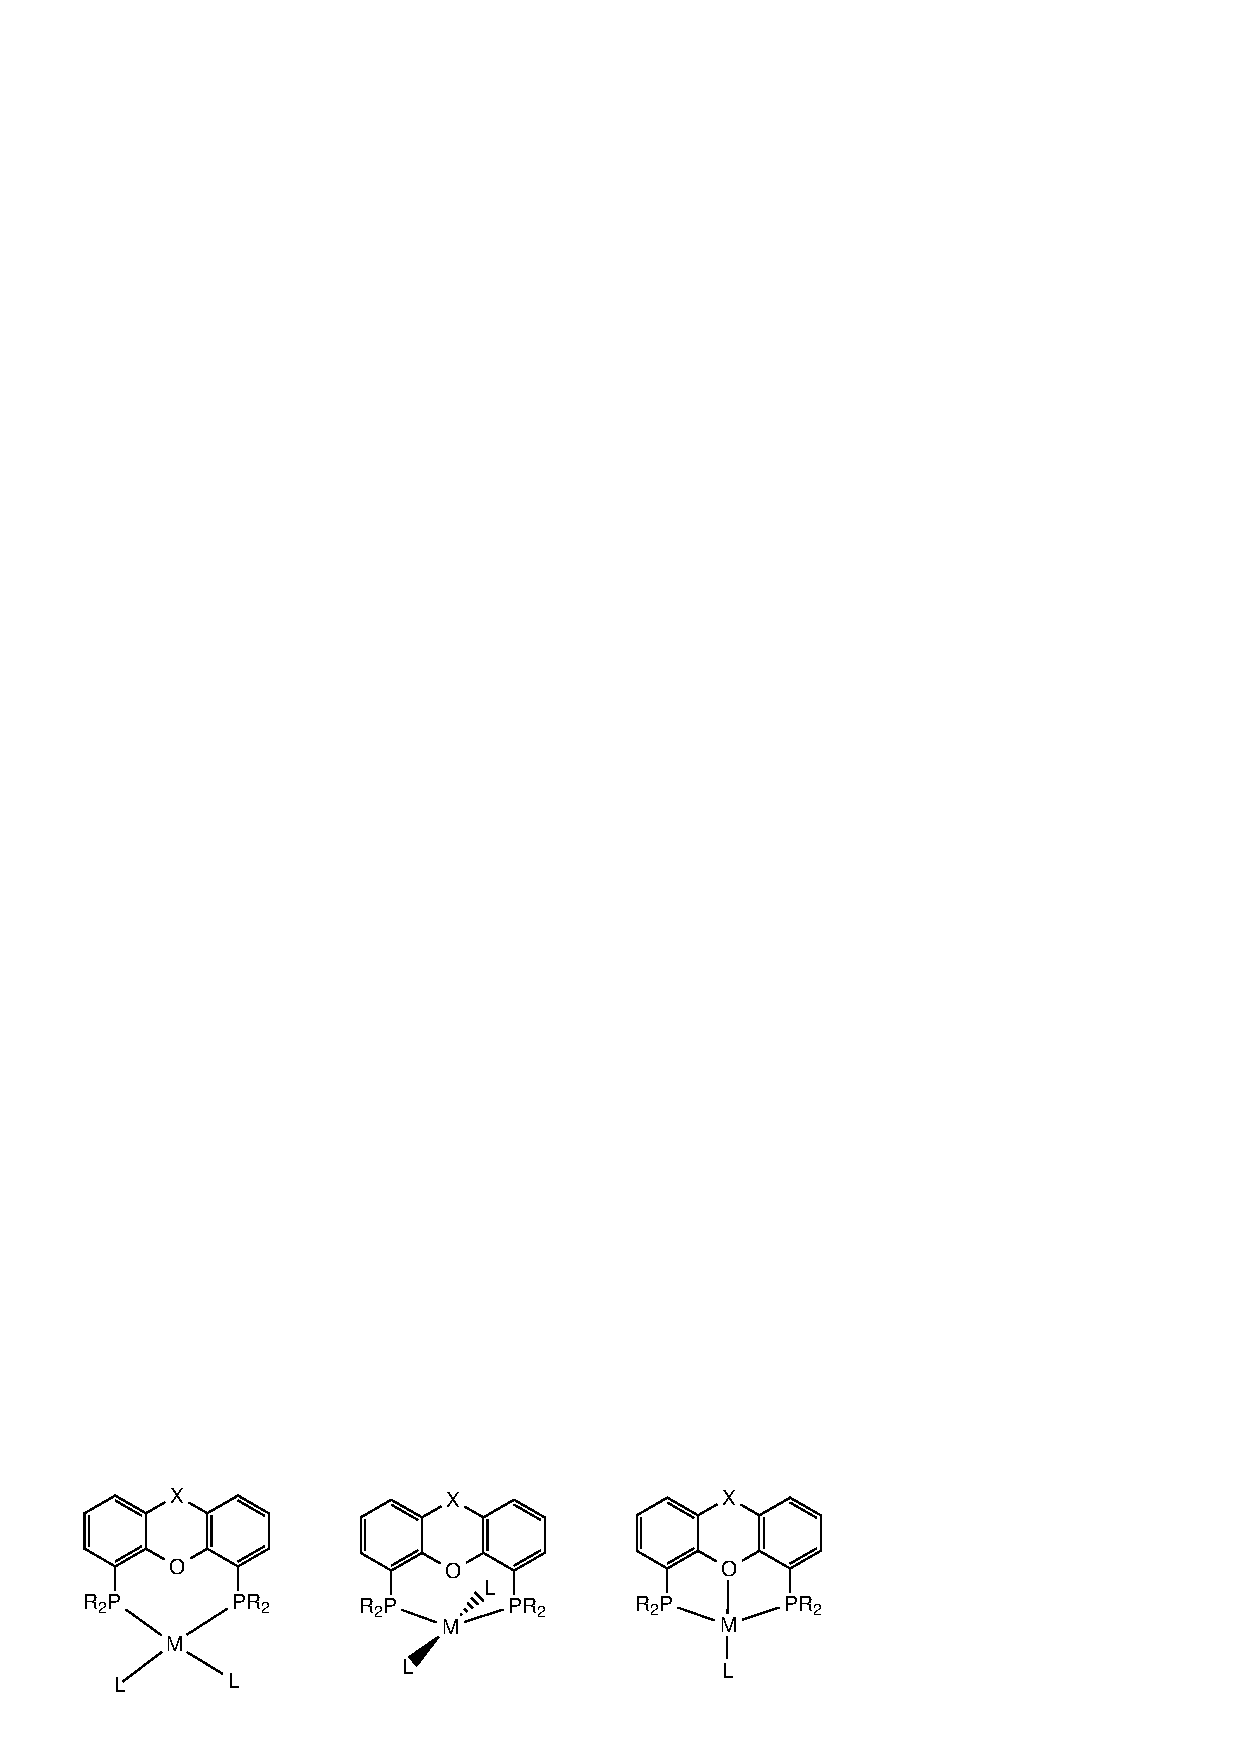
\includegraphics[width = 0.5\textwidth]{../Figures/Bondingmodes.pdf}
\caption[Bonding in organometallic complexes]{Bonding in organometallic complexes}
\label{Bondingmodes}
\end{figure}

Alkanes are weak $\sigma$-bases and $\pi$-acids.  As such they are very poor ligands for transition metals.\cite{Crabtree1993}  Typically alkanes form $\sigma$-complexes with metals that can $\pi$-backbond.  For successful complexation a low valent metal and the absence of competitive decomposition pathways are required.\cite{Crabtree2001}  Enhanced bonding of alkanes occurs with metals capable of forming enhanced $\pi$-backbonding into the $\sigma$* C-H orbital, similar to that found for molecular hydrogen complexes.\cite{Kubas1988}

The activation of C-H bonds is thought occur \emph{via} a stepwise process involving the coordination of the alkane to the metal to form a $\sigma$-complex, followed by the oxidative cleavage of the C-H bond forming metal-alkyl and metal-hydride bonds.\cite{Labinger2002}  The intermediate  $\sigma$-complexes are highly unstable and until recently their existence had only been inferred by isotope scrambling and the inverse kinetic isotope effect in reductive elimination reactions of alkyl hydrides.\cite{Bernskoetter2009, Labinger2002}  In 2009 Brookhart reported the characterisation of a relatively long-lived rhodium(I) $\sigma$-methane complex.\cite{Bernskoetter2009}  The complex was formed by the protonation of a rhodium methyl complex (Scheme \ref{Sigmamethane}).  At -87~\degrees C the methane is displaced by solvent (\ce{CDCl2F}) with a half-life of 83 minutes.

\begin{scheme}[h]
\centering
\includegraphics[]{../Schemes/Sigmamethane.pdf}
\caption[Formation of a $\sigma$-methane complex]{Formation of a $\sigma$-methane complex.  Ar\ce{^{F}} = \emph{m}-di(trifluoromethyl)phenyl}
\label{Sigmamethane}
\end{scheme}

%$\sigma$-Complexes of methane have been proposed 
%The first example of C-H activation was reported by Dimroth in 1902\cite{Dimroth1902}  Reaction of phenol with a solution of mercury acetate on a steam bath replaced the \emph{ortho} and \emph{para}-protons with a mercury acetate group.  \fixme{more info etc}

C-H activation has developed significantly since the first example of C-H activation by an organometallic complex was reported by Chatt in 1962. \cite{Chatt1962}  Reduction of metal halides by sodium napthalene in the presence of an excess of \gls{dmpe} produced V, Cr, Mo and W complexes of the form \ce{[M(}\gls{dmpe}\ce{)_3]},  and Fe and Co complexes of the form \ce{[M(}\gls{dmpe}\ce{)_2]}.  However, the \ce{[Ru(}\gls{dmpe}\ce{)_2]} analogue gave a hydride complex ``by taking hydrogen from the napthalene.''\cite{Chatt1962}  

Further analysis of the ruthenium system was carried out and published in 1965.\cite{Chatt1965} Reaction of \emph{cis}- or \emph{trans}-\ce{[RuCl2(}\gls{dmpe}\ce{)_2]} with benzene, naphthalene, anthracene and phenylanthracene formed the \emph{cis}-\ce{[RuH(aryl)(}\gls{dmpe}\ce{)_2]} (aryl = phenyl, naphthyl, anthryl and phenanthryl) complexes \emph{via} oxidative addition.\cite{Chatt1965}  The activation is reversible, as reactions of the complexes with hydrochloric acid yielded hydrogen gas, the aromatic starting material and \emph{cis}-\ce{[RuCl2(}\gls{dmpe}\ce{)_2]} (Equation \ref{ChattCH}).  The C-H activation to form the complexes was selective for example, in the reaction with naphthalene the activation occurred exclusively at the 2-position.

\vspace{-0.6 cm}
\begin{equation}
\ce{[RuH(C10H7)(dmpe)2] + 2HCl} \longrightarrow \ce{[RuCl2(dmpe)2] + H2 + C10H8}
\label{ChattCH}
\end{equation}

The naphthyl hydride complex formed by treatment of \ce{[Ru(}\gls{dmpe}\ce{)_2]} with naphthalene thermally decomposed giving a complex with properties consistent with \ce{[Ru(}\gls{dmpe}\ce{)_2]} (Scheme \ref{Chattdmpescheme}).\cite{Chatt1965}  However, infrared spectroscopy showed a signal for a Ru-H at 1791 \percm,  leading to the proposed structure of \ce{[RuH(CH2PMeCH2CH2PMe2)(}\gls{dmpe})], formed by activation of a C-H bond from the \gls{dmpe} ligand.\cite{Chatt1965}  X-ray crystallography later allowed the reformulation of the structure to the analogous dimer.\cite{Crabtree2004}  However, this species remains the first example of cyclometallation of an sp$^3$ C-H bond.

\begin{scheme}[h]
\centering
\includegraphics[]{../Schemes/Chattdmpescheme.pdf}
\caption[C-H activation reactions reported by Chatt and Davidson]{C-H activation reactions reported by Chatt and Davidson\cite{Chatt1965}}
\label{Chattdmpescheme}
\end{scheme}

The exchange of hydrogen with deuterium in polyalkyl benzenes, polycyclic aromatic hydrocarbons and heterocycles can be catalysed by homogeneous platinum (II) species.\cite{Hodges1968, Hodges1969, Hodges1969b}  Using deutero-acetic acid as a solution in \ce{D2O}, together with DCl or anhydrous tin(IV) chloride to prevent the formation of platinum metal, H/D exchange on the substrate was observed when exposed to \ce{Na2PtCl4} or \ce{K2PtCl4}.\cite{Hodges1968, Hodges1969}  Although the rate of exchange was faster for unhindered aromatic protons, H/D exchange was also observed for alkyl protons.\cite{Hodges1969b}  The rate was fastest for \hbox{\emph{p}-xylene}, \gls{mesitylene}, \emph{m}-xylene and toluene, however exchange of alkyl protons was also observed in \emph{o}-xylene, \gls{hemimellitene} and \gls{durene}.\cite{Hodges1969b}

This activation of alkyl protons inspired Shilov to investigate the C-H activation of alkanes by platinum.  The system carries out oxidation of alkanes such as methane \emph{via} electrophilic activation (Scheme \ref{Shilovcatalyticcycle}).\cite{Labinger2002, Crabtree2001}  The first step involves displacement of a chloride ligand on the platinum by a $\sigma$-methyl followed by oxidative addition and loss  of H$^+$ \emph{via} loss of HCl.  The Pt(II) is then  oxidised to Pt(IV) \emph{via} electron transfer to the \ce{PtCl6}$^{2-}$.  Finally, the complexed methyl undergoes nucleophilic attack from water displacing the \emph{trans} chloride ion to form HCl, methanol and regenerate the catalyst.  The system has shown selectivity for terminal C-H bonds.  For example, in the oxidation of ethanol functionalisation occurs at the methyl to yield ethylene glycol (Equation \ref{Ethyleneglycol}) whilst, all other methods of oxidation will oxidise the hydroxyl functionality.\cite{Labinger1993}  This can be utilised for the one-pot synthesis of ethylene glycol from ethanol.\cite{Sen1994}  However, the selectivity is lost in reaction with 2-propanol which gives only acetone.\cite{Labinger1993}
\vspace{-1.5cm}
\begin{scheme}[h]
\centering
\includegraphics[]{../Schemes/Shilovcatalyticcycle.pdf}
\caption[Platinum catalysed oxidation of alkanes]{Platinum catalysed oxidation of alkanes}
\label{Shilovcatalyticcycle}
\end{scheme}

\begin{equation}
\ce{CH3CH2OH + H2O + PtCl6}^{2-} \longrightarrow \ce{CH2OHCH2OH + PtCl4}^{2-} + \ce{2HCl} 
\label{Ethyleneglycol}
\end{equation}

Although the Shilov system is catalytic in Pt(II), it requires a stoichiometric amount of Pt(IV).  In addition, the Pt(II) catalyst is unstable in solution and eventually precipitates as platinum metal.\cite{Luinstra1995}  This results in an expensive and thus impractical system for industrial application.  The relatively low yields of the system also reduce its industrial viability.\cite{Periana1993}  Furthermore, the reaction produces two equivalents of hydrochloric acid which require disposal at significant cost.\cite{Poliakoff2001}  A number of attempts have been made to replace the Pt(IV) primary oxidant thus making an economically viable system.\cite{Periana1993, Periana1998, Hashiguchi2010}  However, this has proven challenging as most oxidants tend to convert Pt(II) to the inactive Pt(IV).\cite{Crabtree2001}  Additionally, an oxidant is required that will not attack the product alcohol.  

In 1993 Periana reported the use of concentrated sulfuric acid as the primary oxidant and Hg(II) as a catalyst in place of the platinum.\cite{Periana1993}  The Hg(II) is the highest possible oxidation state so further unwanted oxidation of the catalyst is not possible.  Using methane as the feedstock, the system produces methyl bisulfate in a 43\% yield (Scheme \ref{Mercurycatalyticcycle}).  This has the advantage of being highly resistant to oxidation preventing the formation of carbon dioxide. However, the catalysis involves the formation of MeHg(II)$^+$ as an intermediate following activation.  Methyl mercury salts, like most organomercury compounds, are extremely toxic and exhibit accumulation effects in biological systems.\fixme{cite(MethylmercuryMSDS)}  Sulfur dioxide, a significant contributor to acid rain,\cite{Jacobs1999} is also produced as a stoichiometric byproduct of this reaction.  However, the oxidation of sulfur dioxide to sulfuric acid by air is an established industrial process and could be utilised to provide further sulfuric acid for the process.\cite{Periana1993}

%\begin{equation}
%\ce{CH4 + 2H2SO4} \longrightarrow \ce{CH3OSO3H + 2H2O + SO2} 
%\label{Mercuryequation}
%\end{equation}

%Periana 1993 reaction is carried out at 180 degrees
%Periana 1998 reaction is carried out at 100 degrees

\begin{scheme}[h]
\centering
\includegraphics[width = 0.8\textwidth]{../Schemes/Mercurycatalyticcycle.pdf}
\caption[Mercury catalysed oxidation of methane]{Mercury catalysed oxidation of methane}
\label{Mercurycatalyticcycle}
\end{scheme}

Further work by Periana investigated changing the Pt(II) system to improve stability, activity and prevent oxidation to Pt(IV).\cite{Periana1998}  Nitrogen donor ligands were utilised as oxygen systems have high kinetic lability on platinum and phosphorus ligands have poor oxidative and thermal stability.  The use of \emph{cis}- or \emph{trans}-\ce{[PtCl2(NH3)2]} in concentrated sulfuric acid at 180~\degrees C gave 90\% selectivity for methyl bisulfate.  However, the catalyst degraded to insoluble \ce{PtCl2} and \ce{NH4HSO4}.  

In an extension of this work a $\pi$-acidic chelating donor ligand \gls{bpym} was utilised as $\pi$-donor ligands were expected to have lower proton affinity and form stronger Pt-N bonds than the \ce{NH3} ligands used previously.  The \ce{[PtCl2(}\gls{bpym})] complex was tested in 20 \% \ce{SO3} in \ce{H2SO4} at 200~\degrees C for 50 hours.  Some free ligand and HCl was observed, however the solution remained homogenous showing no formation of platinum metal or other insoluble products.  Using \emph{cis}-\ce{[PtCl2(}\gls{bpym})] in the catalytic system at 220~\degrees C for 2.5 hours resulted in 90\% methane conversion with an 81\% selectivity (carbon dioxide forming the major byproduct).\cite{Periana1998}  However, this reaction requires high temperatures and forms significant amounts of carbon dioxide and sulfur dioxide both of which are environmentally hazardous.\cite{Jacobs1999}  The reaction proceeds \emph{via} a slightly different mechanism to the mercury system (Scheme \ref{PerianaPtcycle}) with oxidation occurring prior to the functionalisation.\cite{Periana1998}

%\begin{figure}[h]
%\centering
%\includegraphics[height = 4cm]{../Figures/bpym.pdf}
%\caption[Structure of \ce{[PtCl2(bpym)]}]{Structure of \ce{[PtCl2(bpym)]}}
%\label{bpym}
%\end{figure}

\begin{scheme}[h]
\centering
\includegraphics[width = 0.9\textwidth]{../Schemes/PerianaPtcycle.pdf}
\caption[Oxidation of methane catalysed by \ce{[PtCl2(bpym)]}]{Oxidation of methane catalysed by \ce{[PtCl2(bpym)]}}
\label{PerianaPtcycle}
\end{scheme}

%Nature of the C-H bond\\ 
%Strong\\
%Highly non-polar\\
%General catalytic attempts\\
%Shilov etc.\\

\subsection{Alkane dehydrogenation}

Alkane dehydrogenation is an alternative approach that combines the activation and functionalisation into a single step.  This methodology was developed from the \hbox{organometallic} complexes such as Wilkinson's\cite{Osborn1966} and Crabtree's\cite{Crabtree1979b} catalysts (Figure \ref{Wilkinsoncrabtree}) that are utilised as homogeneous hydrogenation catalysts.  Wilkinson's catalyst was the first homogeneous hydrogenation catalyst with comparable rates to the heterogeneous counterparts and has become very widely utilised in organic synthesis.\cite{Knowles2003}

\begin{figure}[h]
\centering
\includegraphics[]{../Figures/Wilkinsoncrabtree.pdf}
\caption[Wilkinson's and Crabtree's catalysts]{Wilkinson's (a) and Crabtree's (b) catalysts}
\label{Wilkinsoncrabtree}
\end{figure}

Crabtree reported a number of hydrogenation catalysts based on Wilkinson's catalyst in 1977.\cite{Crabtree1977} The most active of these, \ce{[Ir(cod)(PCy3)(py)]PF6} (Figure \ref{Wilkinsoncrabtree} b, \gls{cod} = 1,5-cyclooctadiene, \gls{Cy}~=~cyclohexyl, \gls{py} = pyridyl) has become known as Crabtree's catalyst.\cite{Cui2005}  This catalyst is active for the hydrogenation of a range of \hbox{mono-,} di-, \hbox{tri-,} and \hbox{tetra-substituted} alkenes with turnover frequencies (\glspl{TOF}) of 6400, 4500, 3800 and 4000 for hex-1-ene, cyclohexene, 1-methylcyclohexene and 2,3-dimethylbut-2-ene respectively.\cite{Crabtree1979b}  Crabtree's catalyst is useful for the hydrogenation of tri- and tetra-substituted alkenes for which Wilkinson's catalyst is inactive.\cite{Cui2005}

A catalytic system lowers the activation energy for a reaction, hence both the forward and reverse reactions will be catalysed.\cite{Crabtree2001}  This realisation led Crabtree to test an iridium system for dehydrogenation of alkenes.\cite{Crabtree1979}  The dehydrogenation would normally be strongly endothermic so the substrates were chosen to give products that would bind strongly to the metal to improve the thermodynamics of the reaction.  In the presence of \ce{[IrH2(alkene)2(PPh3)2]+} and 3,3-dimethylbut-1-ene (as hydrogen acceptor) the dehydrogenation of cyclooctene, [2.2.2]bicyclooctene, cyclopentene and cyclohexene were carried out successfully to give complexes of the type \ce{[Ir(diene)(PPh3)2]+} and \ce{[Ir(Cp)H(PPh3)]+} (Cp = cyclopentadienyl).\cite{Crabtree1979}  The dehydrogenation of alkanes was also possible with the system.  The dehydrogenation of cyclopentane to form the cyclopentadienyl complex gave a 30\% yield after 18 hours, whilst the dehydrogenation of cyclooctane to the cyclooctadiene complex gave a 70\% yield after only 4 hours.\cite{Crabtree1979}

Felkin reported a rhenium complex capable of dehydrogenating linear alkanes to dienes.\cite{Baudry1982}  In the presence of \ce{[ReH7(PAr3)2]} (Ar = \emph{p}-\ce{MeC6H4}) and 3,3-dimethylbut-1-ene, \emph{n}-pentane was dehydrogenated to form a diene complex (Scheme \ref{Pentanedehydrogenation}).  Treatment of this complex with \ce{P(OMe)3} produced pent-1-ene with a yield of 45\%.  This was extended to the linear isomers of hexane, heptane and octane.\cite{Baudry1984}  Although pentane can form only one conjugated diene complex, hexane and heptane can give two, whilst octane can give three.  However, in all cases upon treatment of the complex with \ce{P(OMe)3} the terminal alkene was formed with a selectivity of over 95\%.\cite{Baudry1984}  

\begin{scheme}[h]
\centering
\includegraphics[]{../Schemes/Pentanedehydrogenation.pdf}
\caption[Dehydrogenation of pentane]{Dehydrogenation of pentane reproduced from Felkin et al.\cite{Baudry1982}}
\label{Pentanedehydrogenation}
\end{scheme}

Wilkinson's catalyst (figure \ref{Wilkinsoncrabtree}b) has also been utilised as a dehydrogenation catalyst.\cite{Fujii1990}  The dehydrogenation of cyclooctane to give cyclooctene by \ce{[RhCl(L)3]} (L = \ce{PPh3} or P(\emph{p}-\ce{tolyl)3}) was carried out at reflux (151~\degrees C) without the need for a hydrogen acceptor.  The high temperature of the reaction mixture is sufficient to allow the removal of molecular hydrogen from the reaction mixture.\cite{Fujii1990}  The reaction rates obtained with this system were low, the highest with L = P(\emph{p}-\ce{tolyl)3} was only 1.24 h\ce{^{-1}} with a L/Rh ratio of 8.\cite{Fujii1990}

Crabtree utilised this acceptorless methodology to test the catalytic activity of iridium complexes.\cite{Aoki1993}  \ce{[IrH2L(PCy3)2]} (L = \ce{O2CCF3}, \ce{O2CC2F5} and \ce{O2CPhCH2}) were active for the dehydrogenation of cyclooctane under reflux with initial turnover frequencies of 1.41, 1.05 and 0.22 \ce{h^{-1}} respectively.  However, the complexes were unstable with deactivation half lives of 15, 34 and 14 hours respectively.\cite{Aoki1993}  Alternate methods to remove the hydrogen were also tested.  Using perfluorodecalin as a solvent allowed for more effective hydrogen removal due to the higher volatility compared to cyclooctane.  This resulted in poor activity with a turnover frequency of 0.24 \ce{h^{-1}} using \ce{[IrH2(O2CCF3)(PCy3)2]} as catalyst.  Bubbling inert gas was unsuccessful with cyclooctane as a substrate as a large amount of the substrate was lost.  However, using the less volatile cyclodecane a turnover frequency of 0.48 \ce{h^{-1}}  was obtained.\cite{Aoki1993}

%\fixme{Goldman reference 4 from Gupta1996 had an improved non-pincer system}

\section{Pincer ligands}

Recently, the so-called pincer ligands have attracted a great deal of research attention due to their unique balance of stability and reactivity.\cite{Becerra2009}  Pincer ligands are tridentate ligands that bind in a meridional fashion, examples of which are given in Figure \ref{Pincernaming}.  Pincer ligands are named based on their donor atoms such as, PCP, NCN, and POP.  If the groups between the donor atoms contain heteroatoms then these may be included in the naming also, for example POCOP.  The pincer ligands may be anionic (as with PCP ligands) or neutral (PNP and POP).\cite{Vlugt2009, Kataoka1995}  Although phosphines are the most common donor groups, amines,\cite{Singleton2003} imines,\cite{Takenaka2005} thioethers\cite{Zim2000} and N-heterocyclic carbenes\cite{Hahn2007} have all been reported.

\begin{figure}[h]
\centering
\includegraphics[]{../Figures/Pincernaming.pdf}
\caption[Naming of pincer ligands]{Naming of pincer ligands}
\label{Pincernaming}
\end{figure}

The first reports of pincer ligands were in 1976 by Shaw\cite{Moulton1976} and Alcock.\cite{Alcock1976}  Shaw reported a \emph{tert}-butyl PCP ligand (Figure \ref{Shaw}) and introduced the naming scheme that has become commonplace for pincer ligands.  When reacted with an appropriate metal precursor, complexes formed between the tridentate ligand with nickel, palladium, platinum, rhodium and iridium with chloride, nitrile, hydride and carbon monoxide ligands.\cite{Moulton1976} 

\begin{figure}[h]
\centering
\includegraphics[]{../Figures/Shaw.pdf}
\caption[First reported PCP pincer ligand]{First reported PCP pincer ligand}
\label{Shaw}
\end{figure}

Alcock reported X-ray crystal structures of the first complexes of POP ligands (Figure \ref{Alcock}).\cite{Alcock1976}  These formed rhodium carbonyl complexes that were characterised by X-ray crystallography.  With a single ether group in the backbone it forms a typical pincer complex, bonding through the phosphorus and oxygen atoms.  However, when there are three ether units the phosphorus atoms bond to the rhodium but the oxygen H-bonds to a water molecule that is bound to the rhodium centre.\cite{Alcock1976}

\begin{figure}[h]
\centering
\includegraphics[]{../Figures/Alcock.pdf}
\caption[First reported POP pincer ligand]{First reported POP pincer ligand}
\label{Alcock}
\end{figure}

%Typically the central donor atom E is a carbon from an aromatic ring that binds through C-H activation to form a metallacycle.\cite{Choi2011}  

The different components of pincer ligands have significant influence on the steric and electronic properties and hence their reactivity.\cite{Singleton2003}  Altering the group X (Figure \ref{Pincerligands}) can lead to significant electronic effects mostly through the \emph{trans} influence.\cite{Choi2011}  For example, a carbon donor ligand has a greater \emph{trans} influence than an oxygen donor, so ligands \emph{trans} to X in PXP complexes will be bound more strongly when X~=~O than X~=~C.\cite{Zhu2008} The donor group Y controls the steric environment around the metal centre and the electron density.\cite{Choi2011}  Changing the backbone and other remote groups gives control over the electron density on the metal and can be used to improve solubility properties.\cite{Choi2011}

\begin{figure}[h]
\centering
\includegraphics[]{../Figures/Pincerligands.pdf}
\caption[General representation of pincer ligands]{General representation of pincer ligands}
\label{Pincerligands}
\end{figure}

The tridentate coordination of pincer ligands, typically forming two five-membered metallacycles, imparts significant stability to metal complexes with pincer ligands.\cite{Choi2011}  The stability of the complexes is such that the backbone can undergo functionalisation at the 4-position to trimethylsilane \emph{via} lithiation with \emph{tert}-butyllithium and treatment with trimethylchlorosilane without inducing any decomposition of the platinum complex (Scheme \ref{Stability}).\cite{Albrecht2001}  This inherent stability allows the complexes to act as catalysts for highly endothermic reactions that require high temperatures, such as alkane dehydrogenation.\cite{Choi2011}

\begin{scheme}[h]
\centering
\includegraphics[]{../Schemes/Stability.pdf}
\caption[Functionalisation of an NCN pincer ligand]{Functionalisation of an NCN pincer ligand}
\label{Stability}
\end{scheme}

Coordination complexes of pincer ligands have a large number of applications.  Platinum complexes of an NCN pincer ligand have been utilised as sensors for the detection of sulfur dioxide.\cite{Albrecht2000, Albrecht2000c, Albrecht2001}  Palladium and nickel complexes of a number of pincer ligands have shown activity in cross-coupling reactions.\cite{Hahn2007, Bedford2000, Kimura2006, Zim2000, Obora2006} Theoretical studies have shown potential uses for pincer ligands in water-splitting\cite{Sandhya2011} and nitrogen fixation.\cite{Holscher2007}  However, one of the most prominent uses of pincer ligands is the activation of C-H bonds, typically as dehydrogenation catalysts.\cite{Choi2011, Albrecht2001, Crabtree2001}

%\subsection{Gas sensors}

%Platinum complexes of an NCN pincer (Figure \ref{Gassensors} \fixme{reference the structure correctly}) have been studied in solution or the crystalline state for use in the detection of sulfur dioxide.\cite{Albrecht2000, Albrecht2000c, Albrecht2001b}  In the presence of sulfur dioxide the square planar complex rapidly (less than 50 \si{\micro\second} adsorb the gas to form square pyramidal structures.\cite{Albrecht2000}  The adsorption is accompanied by a dramatic colour change from colourless to bright orange and is reversible upon exposure to a sulfur dioxide free atmosphere.\cite{Albrecht2000}  Dendrimer derivatives (2 and 3, Figure \ref{Gassensors}) can be used to detect sulfur dioxide at concentrations as low as 5 ppm (in a nitrogen atmosphere) \cite{Albrecht2001b}  

%\begin{figure}[h]
%\centering
%\includegraphics[width = \textwidth]{../Figures/Gassensors.pdf}
%\caption[NCN platinum complexes used for sensing \ce{SO2}]{NCN platinum complexes used for sensing \ce{SO2}}
%\label{Gassensors}
%\end{figure}

%These sensors have been studied further for physiological applications.  The complex (Figure \ref{Physiologicalgassensors}) is stable in both acidic and basic aqueous solutions for prolonged periods.\cite{Albrecht2000b}  Testing in conditions known to lead to rapid protein degradation (pH < 1, 50 \degrees C, 5 hours) results in no detectable decomposition.\cite{Albrecht2000b}  The coordination of sulfur dioxide to the complex results in a large shift in the $^{195}$Pt NMR of 1150 ppm (from -3150 to -2000 ppm).\cite{Albrecht2000b}  This could be detected by MRI for medical applications.  These complexes are also being developed for use as molecular switches for opto-electronics.\cite{Albrecht2000c}

%\begin{figure}[h]
%\centering
%\includegraphics[height = 4.5cm]{../Figures/Physiologicalgassensors.pdf}
%\caption[NCN platinum complexes developed for \ce{SO2} sensing in physiological settings]{NCN platinum complexes developed for \ce{SO2} sensing in physiological settings}
%\label{Physiologicalgassensors}
%\end{figure}

%\subsection{Cross-coupling reactions}

%Coordination complexes of pincer ligands also find use as catalysts in carbon-carbon cross-coupling reactions such as the Suzuki, Heck \fixme{etc}.

%Pincer ligands with N-heterocyclic carbene (NHC) donors are becoming more common.\fixme{reference}  The palladium complexes found in figure \ref{CCCPincers} are active for the heck cross-coupling reaction of aryl bromides with styrene and the suzuki cross-coupling of aryl bromides with phenylboronic acid.\cite{Hahn2007}  Using a 1 mol \% catalyst loading the reaction of 4-bromobenzaldehyde and 4-bromoacetophenone with styrene quantitative yields were obtained after 24 hours regardless of the substituent on the ligand.  Using the \emph{n}-butyl derivatised ligand after two hours yields of 84.1, and 60.0 \% were obtained for reaction of styrene with 4-bromobenzaldehyde and 4-bromoacetophenone respectively.   The \emph{n}-butyl derived ligand formed an active palladium catalyst for the Suzuki cross-coupling of phenylboronic acid with 4-bromobenzaldehyde and 4-bromoacetophenone.  Using a 0.1 \% catalyst loading  yields of 50.7 and 48.7 \% respectively were obtained after two hours and quantitative conversion obtained in 24 hours.

%\begin{figure}[h]
%\centering
%\includegraphics[height = 6 cm]{../Figures/CCCPincers.pdf}
%\caption[Palladium complexes with NHC donor pincer ligands]{Palladium complexes with NHC donor pincer ligands}
%\label{CCCPincers}
%\end{figure}

%The palladium complexes with ferrocene based PCP ligands (figure \ref{Ferrocenepalladium}) have been tested for activity in the Suzuki cross-coupling reaction.\cite{Sheloumov2008}  After 4.5 hours the reaction of 4-bromoacetophenone with phenylboronic acid in the presence of 1 and 3 was almost complete with 84 and 84.5 \% yields respectively under homogeneous conditions and quantitative yields under biphasic conditions (decane/\ce{H2O}).  The reaction was much slower with complex 2 with only 66 \% obtained after 15 hours.  Similar activities for all complexes were obtained for the homogeneous reaction of phenylboronic acid with 4-bromoanisole with yields of 77, 79 and 98 \% after 12, 15 and 15.5 hours for 1, 2 and 3 respectively.  However under biphasic conditions complex 2 was much less reactive obtaining a yield of 9 \% after 15 hours compared to 62 and 63.5 \% for 1 and 3 respectively.  The lower activity for complex 2 is thought to be due to the steric bulk of the \emph{tert}-butyl groups though in complex 3 the steric effect is overcome by the electronic influence of the Fe(III) rather than Fe(II).\cite{Sheloumov2008}

%See 

%\begin{figure}[h]
%\centering
%\includegraphics[height = 4.5cm]{../Figures/Ferrocenepalladium.pdf}
% \caption[Palladium complexes of ferrocene pincer ligands]{Palladium complexes of ferrocene pincer ligands}
%\label{Ferrocenepalladium}
%\end{figure}

%Definition\\	
%Naming\\
%Uses of the ligands\\
%Gas sensors\\
%SO2\\
%PCP\\
%POCOP\\
%PNP\\
%POP\\
%Nitrogen activation and fixation\\

\subsection{C-H activation}
%\subsection{Alkane dehydrogenation}

The catalytic dehydrogenation of alkanes has the potential to develop into an important industrial process allowing alkanes to be used as a chemical feedstock, without requiring high temperature cracking or other inefficient processes.\cite{Choi2011}  The first use of pincer complexes for alkane dehydrogenation was reported by Gupta in 1996.\cite{Gupta1996}  The rhodium and iridium dihydride complexes in figure \ref{Dehydrogenationligands} were tested for the dehydrogenation of cyclooctane in the presence of 3,3-dimethylbut-1-ene as hydrogen acceptor.  Rates of 0.8 turnovers h$^{-1}$ at 150~\degrees C were obtained for the rhodium complex, whilst the iridium complex was more active with rates of 82 turnovers h$^{-1}$.\cite{Gupta1996}  The catalysts used were highly stable at this temperature for extended periods and the addition of mercury did not inhibit the reaction indicating a homogeneous system.\cite{Gupta1996}  The higher activity of the iridium complex combined with the high thermal stability has led to a focus on iridium complexes for alkane dehydrogenation.\cite{Choi2011}

\begin{figure}[h]
\centering
\includegraphics[]{../Figures/Dehydrogenationligands.pdf}
\caption[Rhodium and iridium pincer complexes used for alkane dehydrogenation]{Rhodium and iridium pincer complexes used for alkane dehydrogenation}
\label{Dehydrogenationligands}
\end{figure}

The iridium complex (Figure \ref{Dehydrogenationligands}) was also active for the dehydrogenation of cyclic alkanes, tetrahydrofuran and ethylbenzene to give arenes, furan and styrene respectively.\cite{Gupta1997, Gupta1997b}  In all cases the presence of excess 3,3-dimethylbut-1-ene as hydrogen acceptor inhibited the reaction so it was necessary to add this periodically.  A nitrogen atmosphere also inhibited reaction indicating competitive binding of nitrogen and alkane to the active site.\cite{Gupta1996, Gupta1997, Gupta1997b}  The iridium complex is also active for the dehydrogenation of cyclooctane and cyclodecane under acceptorless conditions.\cite{Xu1997}  A solution of fresh catalyst could be poisoned by addition of 10\% alkene rendering the catalyst inactive and indicating that the reduction of activity over time is not due to catalyst decomposition.\cite{Xu1997}

A mechanism for the alkane transfer dehydrogenation (Scheme \ref{Dehydrogenationcatalyticcycle}) has been elucidated \emph{via} a kinetics study by Goldman.\cite{Renkema2003}  The 3,3-dimethylbut-1-ene inserts into an iridium hydride bond, which is followed by reductive elimination to give the alkane.  The substrate undergoes oxidative addition to the iridium centre, which is followed by $\beta$-hydride elimination to give the alkene product and regenerate the iridium-dihydride.  With a limited concentration of 3,3-dimethylbut-1-ene (as is typical for these reactions) the rate determining step is the hydrogenation of the acceptor rather than C-H activation of the alkane, however with an excess of acceptor the rate determing step is the reaction with the cyclooctane.\cite{Renkema2003}  

\begin{scheme}[h]
\centering
\includegraphics[]{../Schemes/Dehydrogenationcatalyticcycle.pdf}
\caption[Proposed mechanism for transfer dehydrogenation]{Proposed mechanism for transfer dehydrogenation}
\label{Dehydrogenationcatalyticcycle}
\end{scheme}

The three-coordinate [Ir(PCP)] intermediate formed following C-H elimination (Figure \ref{Dehydrogenationcatalyticcycle}) was proposed on the basis of an NMR study showing that the dihydride complex will react with 3,3-dimethylbut-1-ene to give the \emph{trans}-2-(\emph{tert}-butyl)vinyl complex that is in equilibrium with [Ir(PCP)] on an NMR timescale.\cite{Kanzelberger2000}  A more recent study has reported this resting state of the complex as the $\pi$-alkene complex and it is likely that both occur depending on the concentration of the hydrogen acceptor.\cite{Choi2011}  Studies into the acceptorless reaction have shown a similar mechanism.\cite{Krogh2002, Krogh2002b}  In this case the rate determining step is the thermolytic loss of \ce{H2} to give the active dehydrogenation complex [Ir(PCP)].  The inhibition of activity resulting from a build-up of alkene is likely due to the formation of the $\pi$-alkene complex and increased rate of the reverse reaction.\cite{Krogh2002, Krogh2002b}

Introduction of electron-donating groups such as \ce{OCH3} in the \emph{para}-position (Figure \ref{DFTpincers}) was shown to favour oxidative addition of an alkane to the 14-electron [Ir(PCP)] complex whilst disfavouring further addition of alkane to the \ce{[(PCP)Ir(R)(H)]} complex.\cite{Krogh2002c}  In the acceptorless dehydrogenation of cyclodecane at reflux (201 \degrees C) the electron-donating \ce{OCH3} pincer complex achieved 820 turnovers in 48 hours compared to 360 with a hydrogen in the \emph{para}-position.\cite{Zhu2004}   However, in dehydrogenation of \emph{n}-undecane at 196 \degrees C little difference was seen between the H and \ce{OCH3} substituted ligands with turnovers of 76 and 91 respectively after 4 hours.  The less sterically bulky isopropyl derivative (with \ce{OCH3} in the \emph{para}-position) was also tested and achieved 2970 turnovers over 48 hours for the dehydrogenation of cyclodecane, indicating that the steric bulk of the ligand has a significant influence of the rate of reaction.\cite{Zhu2004}   In the dehydrogenation of \emph{n}-undecane at 196~\degrees C the isopropyl catalyst was much less active than the \emph{tert}-butyl with only 30 turnovers achieved after 4 hours.  	

\begin{figure}[h]
\centering
\includegraphics[]{../Figures/DFTpincers.pdf}
\caption[Electron-donating pincer ligands]{Electron-donating pincer ligands}
\label{DFTpincers}
\end{figure}

The steric environment imposed by the pincer ligand has a significant impact on the activity towards alkane dehydrogenation.\cite{Choi2011}  A computational and experimental study into this effect was reported by Brookhart in 2009.\cite{Kundu2009}  By exchanging the \emph{tert}-butyl groups on the xylene based PCP complex for methyl groups the impact of the sterically bulky \emph{tert}-butyl groups on alkane dehydrogenation could be studied.  Exchanging a single \emph{tert}-butyl results in a decrease in the transition state for the rate determining step ($\beta$-H elimination) of 42 kJmol$^{-1}$.  This was offset slightly by an increase of 17 kJmol$^{-1}$ in the bond strength of but-1-ene to the iridium centre.  Exchanging a second \emph{tert}-butyl for a methyl was calculated to have a much smaller overall impact as the but-1-ene bonds much more strongly to the metal centre.\cite{Kundu2009}  These results were supported experimentally in the transfer dehydrogenation of \emph{n}-octane using 3,3-dimethylbut-1-ene as the acceptor.  With one and two methyls replacing \emph{tert}-butyl groups, 195 and 140 turnovers were obtained respectively, compared to only 53 for the unmodified ligand.\cite{Kundu2009}

Although the PCP iridium complexes are stable at 150 \degrees C for extended periods, significant decomposition becomes apparent after 24 hours at 200 \degrees C.\cite{Gupta1996}  Ligands based on an anthracene backbone (Figure \ref{Anthraphos}) were developed to achieve a higher level of thermal stability.\cite{Haenel2001}  The ``anthraphos'' ligand forms thermally stable complexes with decomposition occurring at 308 \degrees C for the iridium dihydride complex.  However, in the catalytic dehydrogenation of cyclodecane at 150 \degrees C the complex was less active than the xylene-based systems.  It was proposed that the lack of flexibility in the backbone of anthraphos was responsible for the decreased activity.\cite{Haenel2001}

\begin{figure}[h]
\centering
\includegraphics[]{../Figures/Anthraphos.pdf}
\caption[Iridium anthraphos complexes tested for catalytic dehydrogenation]{Iridium anthraphos complexes tested for catalytic dehydrogenation}
\label{Anthraphos}
\end{figure}

The bis-phosphinite (POCOP) pincer ligands in Figure \ref{Phosphinite} were reported independently by Brookhart (R = \ce{^{t}Bu}, X = \ce{OCH3}, \ce{CH3}, H, F, \ce{C6F5}, ArF)\cite{Gottker2004, Gottker2004b} and Jensen (R~=~\ce{^{i}Pr}, X = H) in 2004.\cite{Morales2004}  Brookhart's complexes were tested for activity in the transfer dehydrogenation of cyclooctane at 200 \degrees C using 3,3-dimethylbut-1-ene as hydrogen acceptor.  These complexes displayed high turnover numbers of up to 2041 after 40 hours forming both cyclooctene and 1,3-cyclooctadiene.\cite{Gottker2004}  The cyclooctadiene product spontaneously converts (most likely \emph{via} a disrotatory ring closure of cyclooctatriene) into \emph{o}-xylene and ethylbenzene (Scheme \ref{Benzeneformation}).\cite{Gottker2004}

\begin{figure}[h]
\centering
\includegraphics[]{../Figures/Phosphinite.pdf}
\caption[Iridium POCOP complex]{Iridium POCOP complex}
\label{Phosphinite}
\end{figure}

\begin{scheme}[h]
\centering
\includegraphics[]{../Schemes/Benzeneformation.pdf}
\caption[Reaction of cyclooctene to form alkylbenzenes]{Reaction of cyclooctene to form alkylbenzenes}
\label{Benzeneformation}
\end{scheme}

The electronic influence of the pincer ligand can also have a dramatic impact on the catalytic activity.  A ruthenium PCP complex with electron-withdrawing \ce{CF3} substituents on the phosphorus atoms (Figure \ref{ElectronwithdrawingPCP}) was tested for transfer and acceptorless dehydrogenation of cyclooctane.\cite{Gruver2011}  The catalyst achieved 186 turnovers at 200 \degrees C after only 30 minutes of transfer dehydrogenation and 10 turnovers in 60 minutes under acceptorless conditions.  This complex was prone to decomposition due to the high temperatures used.  However, the presence of oxygen, nitrogen and water resulted in no significant change to the catalysis which is a significant advantage over other systems.  

\begin{figure}[h]
\centering
\includegraphics[]{../Figures/ElectronwithdrawingPCP.pdf}
\caption[Ruthenium complex of an electron-withdrawing PCP ligand]{Ruthenium complex of an electron-withdrawing PCP ligand}
\label{ElectronwithdrawingPCP}
\end{figure}

Pincer complexes based on metallocenes have also been synthesised and tested for use in alkane dehydrogenation (Figure \ref{Metallocenepincers}).\cite{Kuklin2006}  These complexes have much higher activity than those previously reported.  Turnover numbers of 3300 and 2571 were obtained after eight hours for the iron and ruthenium metallocenes, respectively in the transfer dehydrogenation of cyclooctane with 3,3-dimethylbut-1-ene as hydrogen acceptor at 180 \degrees C.  This compares with 1843 for the iridium POCOP pincer complex (Figure \ref{Phosphinite}) when tested in the same conditions.  The increased activity was proposed as being due to less steric hindrance of the metal centre compared to the POCOP complex.\cite{Kuklin2006}

\begin{figure}[h]
\centering
\includegraphics[]{../Figures/Metallocenepincers.pdf}
\caption[Metallocene based pincer ligands]{Metallocene based pincer ligands}
\label{Metallocenepincers}
\end{figure}

\subsection{Alkane metathesis}

Alkene metathesis is a well-known chemical transformation where the groups of two alkenes are exchanged in the presence of an appropriate catalyst.\cite{Astruc2005}  Alkane metathesis follows the same general principle; the exchange of alkane fragments to produce an array of longer and shorter alkanes.\cite{Choi2011}  Although this was first studied from a heterogeneous perspective,\cite{Burnett1973, Vidal1997, Basset2005} more recently homogeneous pincer complexes have been utilised.\cite{Goldman2006}

%Shell higher olefins process

The first alkane metathesis catalysts were heterogeneous mixtures of dehydrogenation/ hydrogenation and metathesis catalysts.\cite{Burnett1973, Vidal1997}   A mixture of tungsten oxide on silica and platinum metal on alumina formed an active alkane metathesis catalyst.\cite{Burnett1973}  The platinum metal dehydrogenates the alkane, which then reacts in an alkene metathesis reaction, followed by hydrogenation by the platinum to form shorter and longer alkanes.  When exposed to \emph{n}-butane a mixture of 24.7, 37.6, 15.9 and 8.6\% of \ce{C3}, \ce{C4}, \ce{C5} and \ce{C6} linear alkanes was obtained with small amounts of branched and higher alkanes.  However, this system required high temperature (400 \degrees C) and was very sensitive to poisoning by water, ammonia, oxygen and hydrogen sulfide.\cite{Burnett1973}

A tantalum hydride catalyst on silica was more successful with catalysis occuring at room temperature.\cite{Vidal1997}  This system followed a slightly different mechanism, shown in Scheme \ref{Tantalumcatalyticcycle}.  The first step involves coordination to the tantalum \emph{via} loss of hydrogen gas.  This is followed by addition of further alkane to form a metallacycle intermediate that rearranges to give the longer chain product and a tantalum methyl species.  This can react with further alkane to form methane and regenerate the catalytic tantalum alkyl species.  This system is active towards a number of alkanes giving a statistical distribution of longer and shorter alkanes, however the turnover numbers obtained were low; 46, 47, 66, 17 and 12 for ethane, propane, butane, isobutane and pentane respectively.\cite{Vidal1997}

\begin{scheme}[h]
\centering
\includegraphics[width = 0.7\textwidth]{../Schemes/Tantalumcatalyticcycle.pdf}
\caption[Catalytic cycle for alkane metathesis by a heterogeneous tantalum catalyst]{Catalytic cycle for alkane metathesis by a heterogeneous tantalum catalyst}
\label{Tantalumcatalyticcycle}
\end{scheme}

The use of pincer complexes for alkane metathesis has typically followed the tandem alkane dehydrogenation and alkene metathesis protocol (Scheme \ref{Tandemmetathesis}).\cite{Choi2011} Combining an iridium pincer dehydrogenation catalyst with the Schrock alkene metathesis catalyst (Figure \ref{PCPSchrock}) gave active catalysts with turnover numbers of 135, 205 and 125 after 24 hours for the conversion of \emph{n}-hexane using pincer complexes (a) (with L = \ce{C2H4}, \ce{H2}) and (b) respectively.\cite{Goldman2006}  The activity was limited by degradation of the alkene metathesis catalyst as reaction resumed upon further addition of Schrock's catalyst.  A major advantage of this catalytic system is the selective formation of linear alkanes as no branched or cyclic alkanes were detected.\cite{Goldman2006}

\begin{scheme}[h]
\centering
\includegraphics[]{../Schemes/Tandemmetathesis.pdf}
\caption[Alkane metathesis \emph{via} transfer hydrogenation and alkene metathesis]{Alkane metathesis \emph{via} transfer hydrogenation and alkene metathesis}
\label{Tandemmetathesis}
\end{scheme}

\begin{figure}[h]
\centering
\includegraphics[]{../Figures/PCPSchrock.pdf}
\caption[Transfer hydrogenation and alkene metathesis catalysts]{Transfer hydrogenation and alkene metathesis catalysts}
\label{PCPSchrock}
\end{figure}

Replacement of Schrock's catalyst with a heterogeneous alkene metathesis catalyst was tested to increase the stability.  This \ce{Re2O7}/\ce{Al2O3} catalyst was more stable than Schrock's catalyst and showed a higher level of activity with 125 turnovers achieved with complex (b) (Figure \ref{PCPSchrock}) and 180 for complex (c) in 3 hours for the conversion of \emph{n}-decane.\cite{Goldman2006}  However, the activity of the phosphinite complexes was reduced with (a) achieving only 15 turnovers in 3 hours.  Although a high level of selectivity with complexes (b) and (c) for terminal alkenes has been reported for the dehydrogenation,\cite{Liu1999} the product distribution (Figure \ref{GCdistribution})  shows no preference for ethane, which would occur if this was the case.  Either isomerisation of the terminal alkene to form internal alkenes prior to metathesis, or further reaction of the alkane products must occur to account for the observed product distribution.\cite{Goldman2006, Choi2011}

\begin{figure}[h]
\centering
\includegraphics[width = 0.65\textwidth]{../Figures/GCdistribution.pdf}
\caption[GC trace of products obtained from alkane metathesis of \emph{n}-decane]{GC trace of products obtained from alkane metathesis of \emph{n}-decane reproduced from Goldman et al.\cite{Goldman2006}}
\label{GCdistribution}
\end{figure}

\subsection{POP pincer ligands}

Although one of the first pincer ligands reported was a POP pincer,\cite{Alcock1976} this type of ligand has not been studied as extensively as the PCP and PNP analogues.  The osmium trichloride complex of \gls{dbf}(P$^i$\ce{Pr2)2} (Figure \ref{Osmiumdbf}) formed in 98\% yield when the ligand was reacted with the commercially available \ce{OsCl3}$\cdot{}$3\ce{H2O} under reflux.\cite{Asensio2010}  When the ligand is reacted with \ce{OsCl2(DMSO)4} (DMSO = dimethylsulfoxide) the \emph{trans}-dichloro \gls{DMSO} complex (Scheme \ref{Osmiumdbfscheme}) is formed.\cite{Esteruelas2011} This complex can be converted to trihydridechloride and tetrahydride osmium complexes upon reaction with hydrogen gas in the presence of triethylamine or sodium hydrid,e respectively.  The tetrahydride complex is an active catalyst for the coupling of amines and alcohols to give imines achieving a 98\% yield after 3 hours for the coupling of benzyl alcohol and aniline.  Lower yields of 49 and 54\% were obtained when the \gls{DMSO} and trihydride complexes were used.\cite{Esteruelas2011}

\begin{figure}[h]
\centering
\includegraphics[]{../Figures/Osmiumdbf.pdf}
\caption[Osmium trichloride complex of \ce{dbf(P^{i}Pr2)2}]{Osmium trichloride complex of \ce{dbf(P^{i}Pr2)2}}
\label{Osmiumdbf}
\end{figure}

\begin{scheme}[h]
\centering
\includegraphics[]{../Schemes/Osmiumdbfscheme.pdf}
\caption[Reaction of osmium complexes of \ce{dbf(P^{i}Pr2)2}]{Reaction of osmium complexes of \ce{dbf(P^{i}Pr2)2}}
\label{Osmiumdbfscheme}
\end{scheme}

A theoretical study has suggested that POP pincers could be utilised as ligands for ruthenium catalysed synthesis of ammonia from nitrogen and hydrogen gases.\cite{Holscher2007}  The PNP and PSP ligands (Figure \ref{Theoreticalammonia}) have much higher activation barriers for the formation of the active catalytic species than the POP ligands.  Theoretical studies into Shilov chemistry have shown that the presence of an oxygen or nitrogen ligand \emph{trans} to the methane results in much lower activation barriers.\cite{Zhu2009}  The two-step process for C-H activation involves the loss of a ligand followed by coordination of the methane.  The C-H activation has no discernible energy barrier when an oxygen ligand is present in the \emph{trans}-position, however the intial loss of the ligand is much faster for ligands with a higher \emph{trans}-influence making the nitrogen donors much better overall.  Given a system where other factors promoted the loss of the ligand (such as steric bulk) it may be possible that the oxygen-donor ligands are better overall.  

\begin{figure}[h]
\centering
\includegraphics[]{../Figures/Theoreticalammonia.pdf}
\caption[Pincer ligands studied for catalytic ammonia synthesis]{Pincer ligands studied for catalytic ammonia synthesis}
\label{Theoreticalammonia}
\end{figure}

Research into the effect of different phosphorus substituents on the reactivity of ruthenium POP pincer complexes has been reported.\cite{Major2005}  Reaction of \ce{[RuCl2(}\emph{p}-\ce{cymene)]2} (\gls{cymene} = 1-methyl-4-(1-methylethyl)benzene) with the sterically bulky POP-\ce{^{t}}Bu yielded the five-coordinate complex, [Ru\ce{Cl2}(POP)] (Scheme \ref{RutheniumPOP}).  However, the less bulky POP-\ce{^{i}Pr} formed a dimeric species.  Both species were able to form molecular hydrogen complexes however, with the POP-\ce{^{i}}Pr, the \ce{H2} occupies the site \emph{trans} to the ether whilst it occupies the site \emph{trans} to chloride with the bulkier POP-\ce{^{t}}Bu.  The difference was ascribed to the \ce{H2} occupying the most sterically restrained site in the presence of the POP-\ce{^{t}}Bu as it is the smallest ligand (based on van der Waals radii).  

\begin{scheme}[h]
\centering
\includegraphics[width = \textwidth]{../Schemes/RutheniumPOP.pdf}
\caption[Reactivity of ruthenium POP complexes]{Reactivity of ruthenium POP complexes}
\label{RutheniumPOP}
\end{scheme}

The different reactivity was also observed in reaction of the complexes with nitrogen (Scheme \ref{RutheniumPOP}).\cite{Major2005}  The less bulky POP-\ce{^{i}}Pr formed a complex analogous to the molecular hydrogen complex and the two were readily interconverted.  However, the bulky POP-\ce{^{t}}Bu did not react spontaneously with nitrogen and required chloride abstraction using \ce{NaBPh4} in order to form the five-coordinate complex [RuCl\ce{N2}(POP)]\ce{BPh4}.

%See crabtree2001 for the use of pincers in alkane dehydrogenation
%Cundari papers for methane activation DFT studies
	%Methane activation to Ir(PH3)2Cl is 29 kcal mol-1 more exothermic than addition to the hydride complex
%Krogh2002 in the conclusion says that the influence of electron donating ancillary is very minor

POP ligands also have the potential for hemilability of the central donor group whereby the oxygen can bind reversibly to the metal centre in order to stabilise catalytic intermediates. This has been utilised in the hydroacylation of alkenes and alkynes using a rhodium pincer complex, where the oxygen can bind in order to stabilise important intermediates and prevent the competing decarbonylation reactions from occuring.\cite{Moxham2006, Moxham2008, Pawley2010}  A range of rhodium complexes with \gls{xantphos} or \gls{DPEphos} as ancillary diphosphine ligands were tested for the hydroacylation reaction.\cite{Moxham2006}  The \gls{DPEphos} complexes were more active than the \gls{dppe} complex used for comparison, achieving conversions of 100\% after 30 min and 90 min respectively.  However, the xantphos complex was completely inactive.  The different reactivity is thought to be a result of the flexibility of the backbone.\cite{Pawley2010}  The more flexible \gls{DPEphos} readily exhibits hemilability whilst the less flexible xantphos can form either tridentate or bidentate complexes but does not readily convert between the two.\cite{Moxham2006, Pawley2010}  Utilising a PCP pincer resulted in decomposition whilst a PSP pincer bound too strongly to the metal to allow catalysis to occur.\cite{Moxham2008}

\subsection{Xantphos}
	
First reported in 1995 by Kranenburg et al.,\cite{Kranenburg1995} the diphosphine ligand \gls{xantphos} and its derivatives (Figure \ref{Xantphosligands}) were designed to investigate the influence of the bite angle on catalytic reactions, in particular rhodium catalysed hydroformylation.  The bite angle is the angle between the two phosphorus atoms on the diphosphine and the metal centre as shown in Figure \ref{Biteangle}. Utilising different backbones such as diphenyl ether or dibenzofuran, or varying the group in the xantphos backbone to S, \ce{SiMe2} or \ce{CMe2} altered the sterics of the ligand resulting in a change in the bite angle (Table \ref{Biteangletable}).\cite{Kranenburg1995} 

\begin{figure}[h]
\centering
\includegraphics[]{../Figures/Xantphos.pdf}
\caption[The xantphos class of ligands]{The xantphos class of ligands}
\label{Xantphosligands}
\end{figure}

\begin{figure}[h]
\centering
\includegraphics[]{../Figures/Biteangle.pdf}
\caption[The bite angle]{The bite angle}
\label{Biteangle}
\end{figure}

\begin{table}[h]
\caption[Calculated bite angles for xantphos-type ligands]{Calculated bite angle for xantphos-type ligands}
\label{Biteangletable}
\begin{center}
    \begin{tabular}{l l l}
    \hline
Backbone		& Bite angle (\degrees)	& Flexibility range	\\ \hline
\ce{CMe2}	& 111.7				& 97 - 135\\
S			& 109.4				& 94 - 130\\
\ce{SiMe2}	& 108.7				& 93 - 132\\
DPEphos		& 102.2				& 86 - 120\\
dbfphos		& 131.1				& 117 - 147\\
    \hline
    \end{tabular}
    \end{center} 
    \end{table}

In the hydrocyanation of styrene, ligands with bite angles close to 105\degrees~resulted in high yields and selectivities whilst decreasing the bite angle to 101\degrees or increasing to 110\degrees~led to a much lower activity.\cite{Kranenburg1995b}  The bite angle is thought to influence the reaction by stabilising preferred reaction intermediates and destabilising inactive species.   In the hydrocyanation reaction the bite angle close to 109\degrees~ destabilises square-planar Ni(II) species and stabilises the tetrahedral Ni(0) species, enhancing the reductive elimination step and resulting in a faster reaction.\cite{Kranenburg1995b}

Since the initial studies in hydroformylation and hydrocyanation, transition metal complexes of xantphos and its derivatives have been investigated for use in a range of catalytic systems including allylic alkylation,\cite{Kranenburg1998} CO/ethene copolymerisation,\cite{Freixa2003} and C-C and C-X cross-coupling reactions\cite{Birkholz2009} among others.  In addition, a range of further derivatives of xantphos have been synthesised.  Rhodium complexes of the water-soluble xantham\cite{Buhling1997} and sulfoxantphos (Figure \ref{Xantham}) have been used for biphasic hydroformylation.\cite{Goedheijt1998}

\begin{figure}[h]
\centering
\includegraphics[]{../Figures/Xantham.pdf}
\caption[Water soluble xantphos ligands]{Water soluble xantphos ligands (a) Xantham, (b) Sulfoxantphos}
\label{Xantham}
\end{figure}

Xantphos has a range of potential binding modes (Figure \ref{Xantphosbinding}).  By far the most common is the \emph{cis}-bidentate chelating mode (a) with both phosphorus atoms bonding to the metal.  Less commonly the \emph{trans}-bidentate chelating diphosphine mode (b) is observed.  A third, tridentate binding mode (c) is also possible where the oxygen binds in addition to the two phosphorus atoms.  A recent search of the Cambridge Crystallographic Database revealed 107 X-ray crystal structures of coordination complexes with xantphos derived ligand of these only five exhibited the tridentate binding mode.  A monodentate binding mode is also possible, though it is very rare with only one crystal structure reported to date.\cite{Escalle2009}

\begin{figure}[h]
\centering
\includegraphics[height = 2.5cm]{../Figures/Xantphosbinding.pdf}
\caption[Possible bonding modes of xantphos ligands]{Possible bonding modes of xantphos ligands (a) \emph{cis}-bidentate chelate, (b) \emph{trans}-bidentate chelate, (c) tridentate chelate}
\label{Xantphosbinding}
\end{figure}

Ruthenium complexes of xantphos have been utilised for the activation of dihydrogen to form dihydride complexes (Scheme \ref{Xantphosdihydrogen}).\cite{Lenero2003}  Reaction of [Ru(cod)(cot)] (\gls{cot} = 1,3,5-cyclooctatriene) with the diphosphine in a hydrogen atmosphere led to the formation of the \emph{cis}-dihydride.  Protonation of this complex at low temperature (183 K) formed a molecular hydrogen complex that could eliminate hydrogen gas when allowed to warm to 233 K.  

\begin{scheme}[h]
\centering
\includegraphics[width = 0.9\textwidth]{../Schemes/Xantphosdihydrogen.pdf}
\caption[Reactions of ruthenium hydride complexes]{Reactions of ruthenium hydride complexes}
\label{Xantphosdihydrogen}
\end{scheme}

Xantphos and DPEphos ruthenium complexes displaying the tridentate binding mode exhibit reversible bonding of dihydrogen and dinitrogen, together with irreversible binding of peroxide (Scheme \ref{Gascomplexes}).\cite{Ledger2010}  The molecular hydrogen and nitrogen complexes form upon exposure of a dichloromethane solution of the complex to 1 atm of the appropriate gas at low temperature (180 K).  These complexes were unstable and degraded when exposed to higher temperature.  The peroxide complexes form spontaneously on exposure of a dichloromethane solution to air and are stable under ambient conditions.

\begin{scheme}[h]
\centering
\includegraphics[]{../Schemes/Gascomplexes.pdf}
\caption[Ruthenium xantphos complexes of oxygen, hydrogen and nitrogen]{Ruthenium xantphos complexes of molecular oxygen, hydrogen and nitrogen}
\label{Gascomplexes}
\end{scheme}

\section{Things to add for final thesis}
\begin{itemize}
\item Trans-spanning diphosphine ligands see Bessel2001
\item Miedanar for relationship between bite angle and tetrahedral distortions in Pd and Ni
\item Moxham2006 for hemilabile POP catalysis
\item Singleton2003 "the use of pincer complexes in organic synthesis"
\item Trost1995 "atom economy - homogeneous catalysis leads the way"
\end{itemize}


%\fixme{xantphos use as a pincer ligand}\\
%Osmium, Asensio2010, Esteruelas2011\cite{Asensio2010, Esteruelas2011}\\
%Ruthenium, Ledger2010\cite{Ledger2010}

%!TEX root = Thesis.tex

\chapter{Ligand Synthesis and Properties}
\label{ch:ligands}

The xantphos class of diphosphine ligands (Figure \ref{Xantphosligands}) based on a xanthene or xanthene derived backbone are ubiquitous in coordination chemistry and catalysis.  The bis-(diphenylphosphino)xanthene ligands were the first wide bite-angle ligands to be systematically studied for the impact of their bite-angle on catalysis.\cite{Kranenburg1995}  The derivatives showed significant variations in activity and selectivity in the rhodium catalysed hydroformylation of 1-octene.  Subsequently a large number of derivatives have been reported and they have been studied extensively in different catalytic reactions (for examples see \cite{Kamer2001, Asensio2010, Dieleman2001, Jahromi2012, Birkholz2009, Veen2000b}).  

\begin{figure}[ht]
\begin{center}
\vspace{0.5cm}
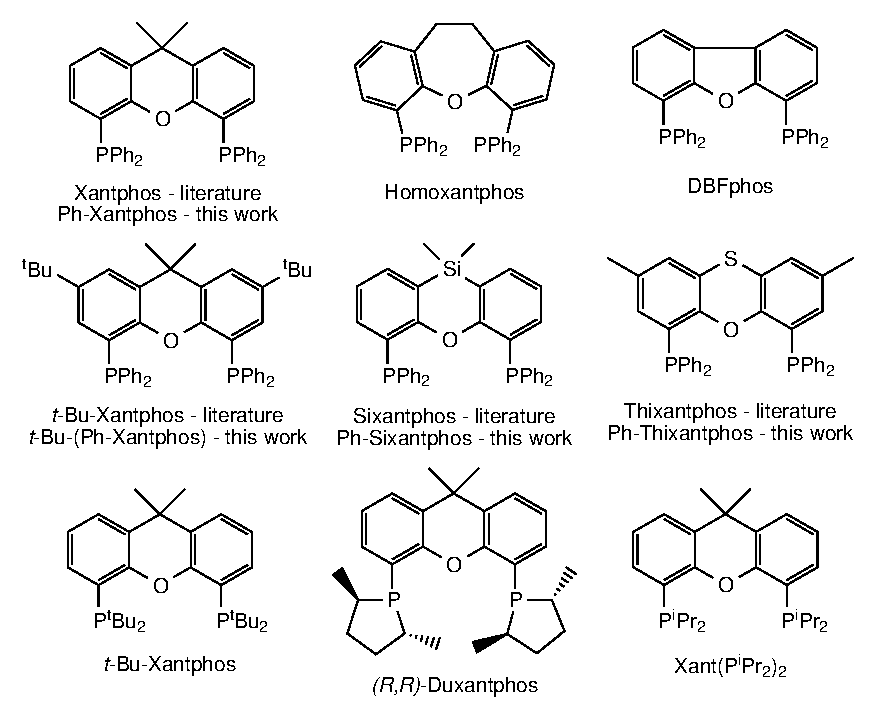
\includegraphics{../Figures/Xantphosligands.eps}
\caption[Examples of the xantphos class of ligands]{Examples of the xantphos class of ligands showing naming and different sites for derivatisation.}
\vspace{0.2cm}
\label{Xantphosligands}
\end{center}
\end{figure}
\vspace{0.2cm}

%A vast number of wide bite-angle ligands based on a xanthene backbone have been synthesised since they were first reported in 1995.\cite{Kranenburg1995, Kamer2001, Esteruelas2011}  The bis-(diphenylphosphino)xanthene ligands were the first wide bite-angle ligands to be systematically studied.  Slight variations in the backbone led to changes in the calculated natural bite-angle.  The derivatives showed significant variations in activity in the rhodium catalysed hydroformylation reacti.  They have since been studied extensively in a range of different reactions \fixme{cite a review or something here} and a number of derivatives have been reported.  

Derivatives of xantphos have focussed mainly on two sites; the bridging group to access a wider range of bite-angles and the phosphine groups.  The phenyl phosphines have been switched for an array for different phosphines including cyclic groups\cite{Veen2000b}, chiral derivatives{\cite{Kamer2001} or changes for solubility.\cite{Buhling1997}  The phosphines have also been switched for different donors including phosphonites,\cite{Dieleman2001} amines, imines, arsines,\cite{Veen2000b} thioethers and others.  Further derivatives with substitutions on the aromatic backbone have also been reported, such as \emph{t}-Bu-(\Phxantphos), or sulfoxantphos,\cite{Goedheijt1998} but are generally less common as changes here have a limited impact due to their distance from the metal.  

Recently an analogue of xantphos has been reported with sterically bulky \tBu{} groups on the phosphines (\tBuXantphos, Figure \ref{Xantphosligands}). First reported in 2005 as a ligand for the palladium catalysed cross-coupling of thiols and aryl bromides or triflates\cite{Mispelaere2005}.  \tBuXantphos{} has since been tested for activity in platinum-catalyzed amination of allylic alcohols\cite{Ohshima2009} and the iron catalysed sp$^3$-sp$^3$ cross-coupling reactions of alkyl halides and alkyl Grignard reagents.\cite{Dongol2007}  However, in each of these cases the complexes were presumed to be formed in the catalytic mixture and were not characterised.  

To date, the only characterised transition metal complexes of \tBuxantphos{} are the series of gold halide complexes [(\tBuxantphos)\ce{Au][AuX2]} where X = Cl$^-$, Br$^-$ or I$^-$.\cite{Partyka2010}  In these structures the \tBuxantphos{} complexes were shown to have large bite angles of 143.0, 142.5 and 143.0\degrees{} for Cl$^-$, Br$^-$ and I$^-$ respectively.  When the same reaction was attempted with the \Phxantphos{} ligands, complexes of the type \ce{[(Xantphos)(AuX)2]} were formed.\cite{Pintado2004, Partyka2010}  These structures clearly indicate the difference between the phenyl and \tBu{} substituted xantphos ligands and the significant impact of the increased steric bulk of the \tBu{} groups on the bonding mode of the ligands.  

The xantphos ligands are widely used in catalysis but \tBuxantphos{} has shown little activity.  This is an indication that the chemistry of the two complexes is substantially different as shown by the only characterised complexes of \tBuxantphos{} reported.  Due to this difference in behaviour further explorations into the coordination activity of \tBuxantphos{} and the reasons for this difference was deemed to be of scientific interest.  Furthermore, the difference in the activity of complexes with \Phxantphos{}, \Phsixantphos{} and \Phthixantphos{} has been previously reported.  Although complexes of \tBuxantphos{} has shown little activity catalytic activity, altering the bridging group, and thus the bite-angle can have a significant impact on the coordination behaviour and the catalytic activity of the complexes produced.  This chapter reports the synthesis of \tBusixantphos{}, \tButhixantphos{} and \tBuxantphos{} along with some of the non-transition metal reactivity of the diphosphines.  

%As these gold complexes are the only examples of characterised tBu-xantphos metal complexes and the phenyl xantphos ligands are so widely utilised the tBu-xantphos ligand system was chosen for further study.  

\section{Ligand Synthesis}\label{section:ligandsynthesis}

In 2002 van Leeuwen \emph{et al.} reported their unsuccessful attempts to synthese \tBuxantphos{} from either the dilithiated backbone or starting with 9,9-dimethyl-4,5-bis(dichlorophosphino)xanthene, suggesting that steric crowding from having two \tBu{} groups on a single phosphorus prevented the successful coupling.\cite{Zuideveld2002}  However, in 2005 a synthesis of \tBuxantphos{} from the dilithiated backbone was reported.\cite{Mispelaere2005}  This synthesis involves lithiation of the backbone using \emph{n}-butyllithium and \gls{TMEDA} in heptane followed by addition of chlorodi-\emph{t}-butylphosphine at 60 \degC{} for 24 hours, generating the product in 38\% isolated yield (Scheme \ref{scheme:Otherligandsynthesis}).

\begin{scheme}[ht]
\begin{center}
\vspace{0.5cm}
\includegraphics{../Schemes/Otherligandsynthesis.eps}
\caption[Literature synthesis of \tBuxantphos]{Literature synthesis of \tBuxantphos{} in heptane.  \emph{i}: \emph{n}-BuLi, \gls{TMEDA}, 15 h. \emph{ii}: \ce{ClP^{t}Bu2}, 60 \degC, 24h.}
\vspace{0.2cm}
\label{scheme:Otherligandsynthesis}
\end{center}
\end{scheme}
\vspace{0.2cm}

%The previously reported synthesis for tBu-xantphos\cite{Mispelaere2005} involved lithiation of the backbone in heptane followed by the addition of chlorodi-\emph{tert}-butyl phosphine and heating to 60\degrees C for 24 hours.  The reportedly air-stable product was obtained and recrystallised from n-propanol in 38\% yield.  Attempts to use this method for the synthesis of tBu-thixantphos yielded a mixture of products.\fixme{check this}

Attempts to utilise the literature method for the synthesis of \tBuxantphos{}\cite{Mispelaere2005} to synthesise \tButhixantphos{} resulted in a number of products which were unable to be identified.  An alternative method using a potassium \emph{tert}-butoxide and \emph{n}-butyllithium ``superbase'' formed a mixture of products from which separation attempts were unsuccessful.  This superbase mixture forms significant amounts of organopotassium compounds, which are more active metallating agents than their organolithium counterparts.  However, organopotassium compounds are also more active in cleavage of ethers.\cite{Bhatt1983}  Hence the mixture of products, may result from cleavage of the ether or thioether bridges resulting in undesired compounds.

%This reference doesn't actually cover organopotassium, just sodium and lithium.

The synthesis of \tButhixantphos{} and \tBusixantphos{} were successfully achieved using the initially reported synthesis of \Phxantphos{}\cite{Kranenburg1995} (Scheme \ref{Ligandsynthesis}).  This method involves the dilithiation of the backbone using \emph{sec}-butyllithium and \gls{TMEDA} followed by reaction with chlorodi-\emph{tert}-butyl phosphine.  Unlike the \Phxantphos{} synthesis which is complete in 16 hours, the synthesis of the \tBu{} ligands required extended periods.  The reaction was allowed to proceed until no further change was determined by NMR (typically 7 days).  NMR analysis of the crude reaction mixture showed the presence of both the mono and diphosphine.  The diphosphine was isolated as white crystals by recrystallisation from \emph{n}-propanol.  The remaining \emph{n}-propanol solution of the monophosphine could be reduced to dryness and then reused for a second lithiation and reaction with chlorodi-\emph{tert}-butyl phosphine to produce more of the desired diphosphine.  

 %carried out in diethyl ether with \gls{TMEDA} using \emph{sec}-butyllithium, added at -78\degrees C followed by addition of the chlorodi-\emph{tert}-butyl phosphine and stirring for 16 hours.  After 16 hours of reaction the NMR spectra showed a mixture of mono and di-substituted products.  The reaction was allowed to proceed until no further change was determined by NMR (typically 7 days).  The reaction invariably produced a mixture of mono and diphosphine.  The diphosphine was separated from the monophosphine by-product by recrystallisation from hot n-propanol and cooling at -16\degC.  The diphosphine was obtained in \fixme{yield} as white crystals.  

\begin{scheme}[ht]
\begin{center}
\vspace{0.5cm}
\includegraphics{../Schemes/Ligandsynthesis.eps}
\caption[Ligand synthesis]{Synthesis of \tBuxantphos{} (X = \ce{CMe2}, R = H), \tButhixantphos{} (X = S, R = Me) and \tBusixantphos{} (X = \ce{SiMe2}, R = H).  \emph{i}: \emph{s}-BuLi, \ce{Et2O}. \emph{ii}: \ce{ClPtBu2}}
\vspace{0.2cm}
\label{Ligandsynthesis}
\end{center}
\end{scheme}
\vspace{0.2cm}

The steric bulk of the \tBu{} groups leads to difficulties in the synthesis of the \tBuxantphos{} ligands.  Reaction with one equivalent of chlorodi-\emph{tert}-butyl phosphine to form the monophosphine is clean and rapid, occurring overnight.  However, the steric bulk of the monophosphine results in a much slower second addition, requiring extended reaction times to allow for significant conversion.  When the reaction is allowed to proceed for longer than one week no additional conversion is observed.  This is likely the result of degradation of either the lithiated monophosphine or the \emph{sec}-butyllithium before the second lithiation can occur.  Over extended periods organolithium reagents cleave diethyl ether resulting in alkanes, alkenes and lithium ethoxide (Scheme \ref{Organolithium}).\cite{Bhatt1983, Gilman1954}  \emph{sec}-butyllithium has been shown to completely react with diethyl ether in one day.\cite{Gilman1954}  Although the reaction between diethyl ether and phenyllithium is slower (half-time of 100 hours), the extended reaction periods required for the second phosphine addition mean that this degradation pathway may limit the reactivity.  \fixme{cite Schlosser organometallics in organic synthesis}

%Between \emph{n}-butyllithium the reaction occurs with a half time of 6 days at 25\degC{}.\fixme{ref}  Although an aryl lithium with an ortho oxygen group would be expected to reaction more slowly with the diethyl ether this is one possible pathway for reaction.  \fixme{does this happen in THF}  

%This is likely a result of the steric bulk of the \emph{tert}-butyl groups hindering the second addition reaction.  However, over time organolithium reagents react with diethyl ether generating lithium ethoxide and ethene (Scheme \ref{Organolithium}).  This reaction occurs with a half time of 6 days at 25\degC{} for \emph{n}-butyllithium.  This is likely the reason for the lack of observed reaction after periods of one week.

\begin{scheme}[ht]
\begin{center}
\vspace{0.5cm}
\includegraphics{../Schemes/Organolithium.eps}
\caption[Reaction of n-butyllithium with diethyl ether]{Reaction of n-butyllithium with diethyl ether}
\vspace{0.2cm}
\label{Organolithium}
\end{center}
\end{scheme}
\vspace{0.2cm}

In order to promote the dilithiation, a preformed sec-butyllithium, \gls{TMEDA} complex was added to a solution of the backbone.  An initial colour change to yellow (\tButhixantphos{} and \tBusixantphos) or green (\tBuxantphos) was observed, indicative of monolithiation.  After stirring overnight this changed to red or yellow respectively.  This colour change gives a clear indication of successful dilithiation.  In order to favour the diphosphine over the monophosphine the lithiated backbone was then added slowly to an ethereal solution of chloro-di-\emph{t}-butylphosphine.  Although a mixture of the mono- and diphosphine was always obtained this order of addition was found to be more successful, resulting in increased yields.

The \tBuxantphos{} ligand obtained using our method had \proton{} and \carbon{} NMR spectra consistent with the literature.\cite{Mispelaere2005} However the \phosphorus{} chemical shift differed by 2.2~ppm (10.2~ppm in this study compared to 12.4 ppm).  The NMR spectra for the reported and the synthesised samples were both obtained in \ce{CDCl3} and referenced to an external 85\% \ce{H3PO4} standard.  Hence the reason for this difference is unclear.  However, as the remainder of the NMR and other characterisation data is consistent, it is likely that the two compounds are identical and a typographical error or otherwise was made in the preparation of the earlier paper.

The synthesis of these ligands utilises directed ortho metallation as first described independently by Gilman and Wittig in 1939 and 1940 respectively.\cite{Gilman1939, Wittig1940} Directed \emph{ortho} metallation uses a heteroatom which can coordinate to the organolithium thereby directing it to the \emph{ortho} sites.  In this case the ether linkage can act as a director for the lithiation.  Once lithiated the electron density on the oxygen stabilises the lithiated site against degradation.  For \tBuxantphos{} and \tBusixantphos{} the oxygen is the only atom present with lone pairs of electrons and thus the lithiation occurs exclusively in the desired positions \emph{ortho} to the oxygen.  However, phenoxathiin has both an ether and a thioether which can both act as \emph{ortho}-directors.\cite{Organolithiummethods}  Previous research shows that in the presence of both ether and thioether groups the lithiation will occur \emph{ortho} to the oxygen.\cite{Turck1997}  However, once the first lithiation has taken place the oxygen is unable to contribute significantly to the second lithiation.  For \tBuxantphos{} and \tBusixantphos{} the influence of the oxygen is still sufficient that the second lithiation occurs in the other ortho position.  However for phenoxathiin the thioether acts as a second directing group and the lithiation occurs \emph{ortho} to the sulfur (Scheme \ref{scheme:transthixantphos}).  The addition of methyl groups in the postion \emph{meta} to the thioether, prevents the sulfur from acting as a director, resulting in the desired \tButhixantphos{} ligand.  

%The methyl groups on the aromatic system of \tButhixantphos{} was found to be important.  The attempted synthesis of a \tButhixantphos{} without methyl groups resulted in substitution ortho to the oxygen and ortho to the sulfur in a transoid configuration (Scheme \ref{Transthixantphos}).  It is likely that using three equivalents of \emph{sec}-butyllithium results in lithiation in three positions, the two ortho to the oxygen and one ortho to the sulfur.  The first addition of phosphine attacks one ortho to the oxygen.  This creates increased steric hindrance at the second site ortho to oxygen so the second equivalent of phosphine preferentially attacks in the least hindered site; ortho to the sulfur.  \fixme{this paragraph may in fact just be lies}.  The oxygen in the bridge of all three ligands acts as a directing group to promote lithiation in the ortho position.  However in the case of \tButhixantphos{} the sulfur can also act as a directing group (though less strongly that the oxygen) this leads to competition for the lithiation site and requires the methyl on the backbone to provide steric hindrance and prevent lithiation ortho to the sulfur.  This difficulty was not encountered with either the \tBuxantphos{} or \tBusixantphos{} ligands.  The carbon and silicon groups are not able to interact with the lithium and promote ortho lithiation so the lithiation occurs exclusively ortho to the oxygen. \fixme{see directed ortho lithiation for more info}

\begin{scheme}[ht]
\begin{center}
\vspace{0.5cm}
\includegraphics{../Schemes/Transthixantphos2.eps}
\caption[Influence of methyl groups on the synthesis of \tButhixantphos]{Influence of methyl groups on the synthesis of \tButhixantphos. \emph{i}: \emph{sec}-BuLi, \ce{Et2O}. \emph{ii}: \ce{ClPtBu2}}
\vspace{0.2cm}
\label{scheme:transthixantphos}
\end{center}
\end{scheme}
\vspace{0.2cm}

%However, the synthesis of \tBusixantphos{} was not problem free.  Given the extended reaction times necessary to obtain the diphosphines, the formed diphosphine is in solution with large volumes of lithium chloride for a substantial amount of time.  NMR analysis of the synthesis of \tBusixantphos{} showed the formation of a significant amount of a compound with a single peak in the \phosphorus{} NMR spectrum at 15 ppm.  No new peaks were observed in the \proton{} NMR spectrum.  However, due to the similarity in the spectra to those of \tBusixantphos H+ we propose that this compound is [Li\tBusixantphos]Cl.  The compound is unchanged through extensive water washing.  Attempts to remove the lithium ion using the lithium specific chelating agent, 12-crown-4, were unsuccessful.  Reaction with tetrafluoroboric acid in order to exchange the lithium for a proton led to the formation of a new species the nature of which could not be determined.  The formation of [Li\tBusixantphos]Cl results in a significant loss of product for the synthesis of \tBusixantphos{} resulting in lower yields than those for \tBuxantphos{} and \tButhixantphos{}.

%It was found the \tBusixantphos{} tended to capture lithium ions between the two phosphorus atoms.  These lithium ions were tightly bound and were retained through several cycles of washing with water.  The nature of this species was confirmed by reaction with a sample of the pure ligand with lithium chloride, resulting in the same product.  \fixme{do this} Attempts to react the lithiated \tBusixantphos{} with tetrafluoroboric acid to exchange the lithium ion for a proton was unsuccessful and instead resulted in possibly a boron trifluoride bound between the two phosphines.\fixme{check this with boron NMR etc.}  Attempts to remove the lithium using the lithium specific chelating agent, 12-crown-4, were unsuccessful.  Due to the inability to remove the lithium this represents a source of significant loss of product for the synthesis of \tBusixantphos{} resulting in lower yields than those for \tBuxantphos{} and \tButhixantphos{}.

The NMR data of the newly reported \tButhixantphos{} and \tBusixantphos{} ligands are consistent with expectations (Table \ref{table:ligandNMRdata}).  In both cases a plane of symmetry reduces the number of signals hence showing a single peak in the \phosphorus{} NMR.  The \phosphorus{} chemical shift for \tBuxantphos{} synthesised in this work is 10.2 which differs from the reported value of 12.4\cite{Mispelaere2005}, however the \proton{} and \carbon{} data is consistent.  The \phosphorus{} chemical shifts for the \tBusixantphos{} and \tButhixantphos{} ligands are observed as singlets at 8.4 and 9.5 respectively.  The \proton{} NMR for the aromatic system is as expected, with two singlets present for \tButhixantphos, and a doublet, doublet of doublets and a triplet observed for \tBusixantphos{} and \tBuxantphos.  The chemical shift of the methyl substituents differs for each ligand, as expected.  In \tBusixantphos{} the dimethylsilyl group appears at 0.46 ppm, close to the tetramethylsilane reference.  In \tBuxantphos{} the bridgehead methyls appear at 1.57 ppm, within the typical range for organic methyl groups.  The methyl groups in \tButhixantphos{} are evident at 2.25 ppm, consistent with methyl substituents attached to aryl rings.  

\begin{table}[ht]
\small
\caption[Selected NMR Data for Xantphos Ligands]{Selected NMR Data for Xantphos Ligands in \ce{CDCl3}}
\vspace{1em}
\label{table:ligandNMRdata}
\begin{center}
\begin{tabular}{l c c c c c c}
	\toprule
	~\bfseries{Diphosphine} & \bfseries{$\delta$P (ppm)} & \multicolumn{5}{c}{\bfseries{$\delta$H (ppm)}} \\
	\midrule		
	~\tBuXantphos\cite{Mispelaere2005}	& 12.4 & 1.21-1.26 & 1.57 s & 7.02 t & 7.38 dd & 7.60 d\\
	~\tBuXantphos{}(This work) 		& 10.2 & 1.21-1.25 & 1.57 s & 7.03 t & 7.38 dd & 7.60 d\\
	~\tBuThixantphos				& 9.5 & 1.22-1.24 & 2.25 s & 6.88 s & 7.29 s & \\
	~\tBuSixantphos				& 8.4 & 1.29 vt & 0.46 s & 7.12 t & 7.53 d & 7.87 d\\ 
	\bottomrule{}
\end{tabular}
\end{center}
\end{table}

The \proton{} NMR data for the \tBuxantphos{} ligands show a complex \ce{X18A}A'\ce{X18}' spin system for the \tBu{} protons.  For a system where the two A atoms (in this case the phosphorus atoms) are strongly coupled this leads to interaction between the three and five bond couplings (e.g. when the phosphorus atoms are in a trans configuration in a metal complex) resulting in a virtual triplet.  However, in this case there is no atom between the phosphorus atoms so we would expect a three-bond and a nine-bond coupling.  A nine-bond coupling is an extremely remote coupling which we would expect to be negligible.  Based on previous reports\cite{Harris1964, Abraham1961} this peak shape with two sharp outer lines and a broad inner peak occurs when the difference between the short and long range couplings is very small but not zero.  For this to occur the phosphines must have some degree of through-space spin-spin coupling through their lone pairs of electrons (for a review of nonbonded spin-spin coupling see Hierso\cite{Hierso2014}).  This is further supported by the difference in the \proton{} spectra for the three ligands; the central peak is sharpest for \tBusixantphos{} then \tButhixantphos{}.  For \tBuxantphos{} some further detail can be seen indicating that this has the weakest through space coupling.  This trend is consistent with the expected changes in the distance between the phosphines upon changing the backbone which will impact the degree of through-space coupling that can occur and therefore the difference in the short and long-range coupling constants.

%include spectra showing the tBu peak?

\section{Bite Angle Calculations}

The steric and electronic properties of diphosphine ligands determines their complexation behaviour with transition metals and can influence the reactivity of the complex, particularly impacting the activity and selectivity in catalytic transformations.\cite{Freixa2003, Birkholz2009}  The xantphos class of ligands were initially investigated as ligands with consistent electronic properties and steric bulk so that the impact of the bite-angle on rhodium catalysed hydroformylation could be studied exclusively.\cite{Kranenburg1995}  Consequently a number of studies have investigated the bite-angle impact on a variety of catalytic conversions (for examples see\cite{Kranenburg1995b, Haaren2001b, Dudle2011b, Fanjul2013, Birkholz2009}).  However, it has since been determined that the bite-angle is a result of both the steric and electronic properties of the ligand.\cite{Freixa2003}

The natural bite-angle (\natbiteangle) was first described by Casey and Whiteker\cite{Casey1990} as a theoretically determined parameter to indicate the preferred chelation angle of diphosphine ligands irrespective of the metal they are coordinating to.  Computationally these are calculated using a rhodium atom at 2.3 \si{\angstrom} and optimising the geometry of the ligand system, the natural bite-angle can then be measured.  This is often used in combination with a flexibility range (the bite-angles that can be obtained within a range of 12.6~\si{\kilo\joule\per\mol}).  

Despite the ubiquity of the natural bite-angle within diphosphine chemistry no studies have investigated whether the natural bite-angle has proven to be an apt predictor of the crystallographically determined bite-angle.  In order to determine the usefulness of the natural bite-angle in determining the coordination bite-angle an investigation into this, using data from the \gls{CSD} was performed.  The results are summarised in Table \ref{table:biteangles} and Figure \ref{Biteanglegraph}.  The natural and median experimental bite-angles show a good correlation described by the equation $\Theta$\sub{exp} $= 1.1013$\natbiteangle $- 5.6972$, ($R^2 = 0.9246$).  Some of the experimental and natural bite-angles that are most relevant to this work show significant differences (for example \tBuxantphos{} \natbiteangle{} = 140\degrees, experimental = 153.317\degrees and \Phsixantphos{} \natbiteangle{} = 109, experimental = 99.165\degrees) this may be due to the low numbers of structures for these ligands (4 and 5 respectively) at which point the metals used will have a significant impact. 

\begin{table}[htb]
\small
\caption[Crystallographic bite-angles for diphosphine ligands]{Crystallographic bite-angles for diphosphine ligands, taken from the Cambridge Crystallographic Data Centre.} 
\vspace{1em}
\label{table:biteangles}
\begin{center}
\begin{tabular}{c c c c c c}
	\toprule
	~~\bfseries{Diphosphine}~~ & \bfseries{Structures} & \bfseries{P-P ($\si{\angstrom}$)} & \bfseries{Range (\degrees)} & \bfseries{Bite-Angle (\degrees)} & \bfseries{$\beta$\sub{n} (\degrees)}\\
	\midrule
	 ~dppm			& 384	& 2.718	& 62.757 - 77.706 	& 71.062 	& 73	\\
	 ~dppe			& 1939	& 3.095	& 71.073 - 92.926	& 83.818	& 78 \\
	 ~dppp			& 3237	& 3.308	& 83.333 - 105.420	& 92.181	& 86 \\ 
	~BINAP			& 146	& 3.296	& 85.9820 - 115.666	& 91.925	& 92 \\
	~dppb			& 127	& 3.391	& 89.447 - 111.491	& 94.240	& 99 \\
	 ~DPEphos		& 101	& 3.844	& 96.094 - 158.531	& 112.691	& 102 \\
	 ~\PhXantphos		& 65		& 3.908	& 98.829 - 153.134	& 108.535	& 111 \\
	 ~BISBI			& 4		& 4.079	& 103.533 - 151.951	& 124.789 & 123 \\
	~Ph-sixantphos		& 5		& 3.691 	& 95.250 - 152.149	& 99.165 & 109 \\
	~Ph-thixantphos	& 3		& 4.021	& 109.528 - 155.050	& 111.724	& 110 \\
	~tBu-xantphos		& 4		& 4.527	& 152.302 - 153.456 & 153.317 & 140 \\
	~dpp-benzene		& 116	& 3.101	& 74.380 - 92.499	& 84.900	& 83\\
	~dppn			& 25		& 3.176	& 79.867 - 93.270	& 86.864	& 82 \\
	~dppx			& 19		& 3.569	& 90.045 - 106.186	& 102.636	& 90 \\
	~dbpe			& 109	& 3.200	& 83.989 - 95.949	& 90.369	& 87	\\
	~dbpp			& 12		& 3.503	& 94.556 - 104.857	& 99.175	& 99	\\
	~dbpx			& 10		& 3.634	& 98.758 - 107.255	& 101.881	& 101 \\
	\bottomrule{}
\end{tabular}
\end{center}
\end{table}

\begin{figure}[htb]
\begin{center}
\vspace{0.5cm}
\includegraphics[width=\textwidth]{../Figures/Biteanglegraphorigin.eps}
\caption[Comparison of the Natural Bite-Angle with the Experimentally Determined Bite-Angle]{Comparison of the Natural Bite-Angle with the Experimentally Determined Bite-Angle.  Trendline $ y = 1.1013x - 5.6972$, Linear regression $R^2 = 0.9246$}
\vspace{0.2cm}
\label{Biteanglegraph}
\end{center}
\end{figure}
\vspace{0.2cm}

In order to determine the potential differences between the \tBu{} and Ph xantphos ligands, the natural bite-angles of the three \tBuxantphos{} ligands were calculated.  Bite-angle calculations are typically carried out using molecular mechanics, in this study we used a \gls{DFT} instead, hence the natural bite-angles of the previously reported \Phxantphos{} series of ligands and \tBuxantphos{} (Table \ref{table:biteanglescalculated}).  The structures were optimised using the B3LYP functional\cite{Becke1993, Lee1988, Vosko1980, Stephens1994} with the def2-TZVP basis set.\cite{Andrae1990, Weigend2005} using a Rh-P distance of 2.315 \si{\angstrom}.  The values calculated using \gls{DFT} are typically larger than those reported using molecular mechanics (Table \ref{table:biteanglescalculated}).\fixme{why?}

%These show good agreement with those calculated using molecular mechanics.  Given the good agreement of our DFT obtained values and the literature values we continued by calculating the bite-angles for the two new ligands \tButhixantphos{} and \tBusixantphos{}.  A number of different bite-angles have been reported for the \Phxantphos{} series, due to different computational set-ups.  

\begin{table}[ht]
\small
\caption[Bite angles of xantphos ligands]{Bite angles of xantphos ligands}
\vspace{1em}
\label{table:biteanglescalculated}
\begin{center}
\begin{tabular}{c c c c}
	\toprule
	~\bfseries{Diphosphine}	&\bfseries{Molecular Mechanics (\degrees)}&\bfseries{Reference}	&\bfseries{DFT (\degrees)}\\
	\midrule		
	~\PhXantphos		~~&~108, 111.7~~	& ~\cite{Birkholz2009}	&~~118.59~~	\\	
	~\PhThixantphos	~~&~110, 109.4~~	& ~\cite{Birkholz2009, Kranenburg1995}&~~118.04~~	\\
	~\PhSixantphos	~~&~108, 108.7~~	& ~\cite{Birkholz2009, Kranenburg1995}&~~111.43~~	\\
	~\tBuXantphos		~~&~140~~		&~\cite{Birkholz2009}~~	&~~159.93~~	\\
	~\tBuThixantphos	~~&~~~			&~~~~			&~~126.98~~	\\
	~\tBuSixantphos	~~&~~~			&~~~~			&~~126.80~~	\\
	\bottomrule{}
\end{tabular}
\end{center}
\end{table}

%  including allylic alkylations\cite{Haaren1999}, rhenium catalysed hydrogenation\cite{Dudle2011b} and the palladium catalysed hydromethoxycarbonylation of ethene.\cite{Fanjul2013}  
%reviews have investigated whether the bite-angle impact is 

The natural bite-angles for the \tBuxantphos{} series of ligands are much larger than for the phenyl substituted ligands.  Given that the remainder of the ligands is unchanged, this effect is due to the impact of the \tBu{} groups.  These groups are more electron donating than the phenyls so may result in more electron density on the phosphorus atoms resulting in an electrostatic repulsion of the two phosphorus atoms.  The \tBu{} groups have a larger steric impact than the planar phenyl rings.  This would result in a larger bite-angle as the steric bulk of the \tBu{} substituents pushes the two phosphorus atoms further apart.  The trend between the two groups is the same with the carbon bridged having the largest \biteangle{} and the silicon bridged having the smallest.

The bite-angles of the \tBuxantphos{} ligands is likely to have a significant impact on their coordination chemistry.  The phenyl ligands form a range of complexes favouring \cis-chelation in square-planar and octahedral complexes, although \emph{trans} square planar complexes have been reported\cite{Petocz2004}.  With bite-angles of 126.8-159.9\degrees{} the ligands will likely prefer trigonal planar coordination environments close to 120\degrees.  However the bite-angles are halfway between the \cis{} and \trans{} coordination angles for square planar complexes which may result in mixtures of products.  The ratio between the two geometries may change depending on which ligand is used with \tBusixantphos{} favouring \cis-coordination while \tBuxantphos{} favours the \trans-coodination.  However, the steric demands of the \tBu{} substituents may promote the \trans{} chelation.  

Diphosphine ligands that exhibit exclusive \trans-chelation have been described in a review as elusive.\cite{Freixa2008}  \PhXantphos{} itself can form \trans-chelates\cite{Petocz2004}, however these form as a mixture of the \cis and \trans isomers rather than forming as the pure \trans isomer.  Only a small number of these \trans-chelates for \Phxantphos{} have been reported compared to the majority of complexes where the \cis-chelate forms.  A limited number of ligands exist that can form \trans-chelates, however, rarer are those that do not form \cis-chelates and rarer still are the truly \trans-chelating ligands with a bite-angle of 180\degrees{} and an undistorted coordination plane. 

The wide bite-angles of these ligands may also result in interesting catalytic activity.  Previously reported uses of \tBuxantphos{} have added the ligand to a metal precusor and formed the catalyst in situ.  However platinum(II), palladium(II) and iron prefer either square-planar or octahedral coordination and if the \tBuxantphos{} ligand coordinated in a \trans{} configuration this may prevent the reductive elimination of other ligands.  Hence although \tBuxantphos{} has not shown activity in catalytic systems to date, these ligands may find more use in systems with metals able to form tetrahedral, trigonal planar, or pyramidal structures such as silver or rhodium, or platinum and palladium(0).

%\section{Oxidation}

%Although previous literature reports \tBuxantphos\cite{Mispelaere2005} as an air-stable solid, this was not the case for at least \tButhixantphos.  The ligands are resistant to oxidation and can be handled in the air for short periods.  However, storage in the air leads to slow oxidation.  

%The ligands appear to be more stable to oxidation using hydrogen peroxide than \Phxantphos{}.  Although the \tBuxantphos{} ligands oxidise slowly in the air which \Phxantphos{} does not; attempts to directly oxidise using a large excess of hydrogen peroxide in acetone requires extended periods of reflux while \Phxantphos{} undergoes complete oxidation after only 1 hour at room temperature.\cite{Jahromi2012}

%However problems were encountered with this as the thioether bridge is also susceptible to oxidation.  As such attempts to oxidise the phosphines of \tButhixantphos resulted in oxidation of one of the phosphine arms and the thioether bridge to a sulfoxide or sulfone resulting in a mixture of products.  

\section{Basicity}
\label{section:ligands:basicity}

During the synthesis of the \tBuxantphos{} ligands, particularly for \tBusixantphos{} a small amount of a by-product was observed by \phosphorus{} and \proton{} NMR spectroscopy.  The \proton{} NMR spectra suggested the presence of an additional proton environment.  Leaving the ligands for extended periods in \ce{CDCl3} resulting in increased amounts of this impurity over time, suggesting that the formed \tBuxantphos{} ligands were undergoing reaction with the solvent rather than the impurity forming in the synthesis of the ligands.  Over time chloroform is known to undergo degradation forming hydrochloric acid.\cite{Yano1977}  Furthermore tertiary phosphines are known to act as Br\o nsted bases, forming phosphonium ions that can be used as components in catalytic reactions.\cite{Netherton2001}  Hence, the identity of these compounds as phosphonium salts seemed likely.

%As discovered during the synthesis of \tBusixantphos{} the ligands have the ability to coordinate small cations.  Although only \tBusixantphos{} coordinated lithium to any significant degree during the synthesis, all three of the ligands are significantly acid sensitive and will react with any adventitious proton source resulting in the protonation at one of the phosphines.  Although stable for short periods in deutero-chloroform, over time chloroform produces hydrochloric acid \emph{via} photo-degradation which readily protonates the ligands

Reaction of the \tBuxantphos{} ligands with either of the strong acids \ce{CHPh(SO2CF3)2} (\pKa = 2.0 in DMSO) or \ce{CH2(SO2CF3)2} (\pKa = 2.4 in DMSO), results in immediate formation of a phosphonium salt (Scheme \ref{Protonation}).  These acids are useful as they are non-hygroscopic solids allowing for accurate stoichiometry.  However, addition of excess acid results in the same product, no evidence for an additional protonation was observed.  The NMR data is consistent with the data for the impurity observed in the synthesis of the \tBuxantphos{} ligands, indicating that the impurity is [\tBuxantphos(H)\ce{]+}.

\begin{scheme}[ht]
\begin{center}
\vspace{0.5cm}
\includegraphics{../Schemes/Protonation.eps}
\caption[Protonation of the ligands using a strong acid]{Protonation of the ligands using a strong acid}
\label{Protonation}
\end{center}
\end{scheme}
\vspace{0.2cm}

Selected NMR data for the phosphonium salts [\tBuxantphos\ce{(H)]+} is given in Table \ref{table:protonatedNMR}.  A broad singlet is present in the \phosphorus{} NMR spectra for the three phosphonium ions shifted slightly downfield of the free ligand.  Similarly half the expected number of peaks is observed in the \proton{} and \carbon{} NMR spectra.  This indicates that although the complex is mono-cationic the system is undergoing a dynamic process such that the two halves of the molecule are equivalent on the NMR timescale.  The most likely process is the exchange of the proton between the two phosphorus atoms.  The \proton{} NMR spectra all show a complex spin system of the type XAA\textprime X for the phosphonium proton, which is further evidence for the dynamic exchange of the proton between the two phosphorus atoms.  

\begin{table}[htbp]
\caption[Selected NMR data for [\tBuxantphos(H){]}\ce{CH(SO2CF3)2}]{Selected NMR data for the [\tBuxantphos(H){]}\ce{CH(SO2CF3)2} compounds}
\label{table:protonatedNMR}
\small
\begin{center}
\begin{tabular}{l c c c}
	\toprule{}
	~~ & \multicolumn{2}{c}{\bfseries{\phosphorus}} & \bfseries{\proton}\\
	\cmidrule(lr){2-3} \cmidrule(lr){4-4}
	\bfseries{Ligand}&\bfseries{$\delta/$ppm}&\bfseries{$\Delta\delta/$ppm}& \bfseries{\ce{H+}$\delta/$ppm}\\
	\midrule{}
	\tBuSixantphos		& 14.3	& 5.9 	& 9.57 \\
	\tBuThixantphos 	& 15.8	& 6.3		& 8.99 \\
	\tBuXantphos		& 17.4	& 7.2		& 8.57 \\
	\bottomrule{}
\end{tabular}
\end{center}
\end{table}

The difference in the rate of exchange of the proton in the three compounds in clearly shown by the \phosphorus{} and \proton{} NMR spectra.  The \phosphorus{} NMR signal is sharpest for \tBusixantphos{} followed by \tButhixantphos{} while \tBuxantphos has a very broad signal.  Indicating the exchange is fastest for \tBusixantphos{} and slowest for \tBuxantphos{}.  The \proton{} NMR spectra (Figure \ref{Protonatedligandsnmr}) show an XAA'X spin system for the phosphonium proton.  The signal appears most like a virtual triplet for \tBusixantphos{} indicating very little different in the coupling constants of the proton with each phosphorus.  For \tButhixantphos{} the central peak has broadened slightly, while in \tBuxantphos{} the central peak is very broad indicating that the difference in the two coupling constants is increasing.  Furthermore the chemical shift of the phosphonium proton is different  for the three systems (\tBusixantphos{} = 9.57, \tButhixantphos{} = 8.99 and \tBuxantphos{} = 8.57~ppm).  This indicates that the \tBusixantphos{} proton is less shielded and thus has a faster rate of exchange while \tBuxantphos{} proton is the most shielded and has the slowest rate of exchange.  This trend is consistent with the bite-angles for the ligands.  \tBusixantphos{} has the smallest bite-angle and thus the two phosphorus atoms are closer resulting in a lower barrier to exchange, whilst \tButhixantphos{} has the largest bite-angle and thus the slowest exchange.  

%The \phosphorus{} NMR spectrum has a single broad signal at 15.8 ppm showing a downfield shift of 6.3 ppm upon protonation.  In the \proton{} NMR spectrum the phosphonium proton comes at 9.0~ppm much higher than other phosphonium ions.  In addition the proton appears as an unusual signal in a 1:2:1 ratio with two sharp outer peaks and a broad inner peak.  The \phosphorus{}, \proton{} and \carbon{} spectra show half of the expected peaks indicating a plane of symmetry through the central bridge of the molecule.  However, the signal for the phosphonium proton only integrates for a single proton.  Together with the broadness of the \phosphorus{} and some of the \carbon{} signals this indicates a dynamic system in solution with proton exchange between the two phosphorus atoms.   \fixme{this data is for the sulfur bridged ligand should I include stuff for silicon as well?} 

\begin{figure}[htb]
\begin{center}
\vspace{0.5cm}
\includegraphics[scale = 0.8, trim = 1.5cm 10cm 4.5cm 5cm, clip]{../NMR/Phosphoniumstacked.eps}
\caption[\proton{} NMR spectra for \tBusixantphos, \tButhixantphos{} and \tBuxantphos{} showing the P-H region]{\proton{} NMR spectra in \ce{CDCl3} at 20\degC{} for \tBusixantphos, \tButhixantphos{} and \tBuxantphos{} (Si, S and C respectively) showing the P-H region}
\vspace{0.2cm}
\label{Protonatedligandsnmr}
\end{center}
\end{figure}
\vspace{0.2cm}


%\begin{figure}[htp]
%\begin{center}
%\vspace{0.5cm}
%\includegraphics[scale=0.85]{../Figures/VTNMR/Protonatedligands.pdf}
%\caption[\proton{} NMR spectra for \tBusixantphos, \tButhixantphos{} and \tBuxantphos{} showing the P-H region]{\proton{} NMR spectra in \ce{CDCl3} at 20\degC{} for \tBusixantphos, \tButhixantphos{} and \tBuxantphos{} (Si, S and C respectively) showing the P-H region}
%\vspace{0.2cm}
%\label{Protonatedligandsnmr}
%\end{center}
%\end{figure}
%\vspace{0.2cm}

The dynamic behaviour of the phosphonium ions was further investigated using variable temperature \phosphorus{} and \proton{} NMR experiments on [(\tButhixantphos)H]\ce{CH(SO2CF3)2} (Figure \ref{VTStBuH})  At room temperature a single peak is present in the \phosphorus{} NMR spectrum.  When heated this peak shifts slightly to higher ppm and becomes sharper.  This single peak indicates that the exchange of the proton between the two phosphorus atoms is occuring rapidly enough that the two phosphorus atoms appear to have the same environment on the NMR timescale.  Cooling below room temperature causes the singlet to broaden significantly with coalescence occurring around -40\degC{}.  At -60\degC{} two signals are present though they are still broad.  One of these signals resolves into a doublet at -80\degC, however the other peak is still very broad ranging from 11-23 ppm.  Given the chemical shift of the free ligand it is likely that the sharp doublet belongs to the unprotonated phosphorus and the broad peak is the protonated phosphorus.  This is also consistent with the shift of the peaks at higher temperature where we observe a shift to higher ppm as the rate of exchange is increased.  

\begin{figure}[h!]
\begin{center}
\vspace{0.5cm}
\includegraphics[scale=0.8, trim = 0cm 6.8cm 0cm 2cm]{../NMR/PhosphoniumVTNMRboth.eps}
\caption[Variable temperature \phosphorus{} and \proton{} NMR data for {[}(\tButhixantphos)H{]}\ce{CH(SO2CF3)2}]{Variable temperature \phosphorus{} (right) and \proton{} (left) NMR data for [(\tButhixantphos)H]\ce{CH(SO2CF3)2}}
\vspace{0.2cm}
\label{VTStBuH}
\end{center}
\end{figure}
\vspace{0.2cm}

%\begin{figure}[h!]
%\begin{center}
%\vspace{0.5cm}
%\includegraphics[scale=0.8]{../Figures/VTNMR/StBuHboth.pdf}
%\caption[Variable temperature \phosphorus{} and \proton{} NMR data for {[}(\tButhixantphos)H{]}\ce{CH(SO2CF3)2}]{Variable temperature \phosphorus{} (right) and \proton{} (left) NMR data for [(\tButhixantphos)H]\ce{CH(SO2CF3)2}}
%\vspace{0.2cm}
%\label{VTStBuH}
%\end{center}
%\end{figure}
%\vspace{0.2cm}

The variable temperature \proton{} NMR data for [\tButhixantphos\ce{H]CH(SO2CF3)2} (Figure \ref{VTStBuH}) shows similar changes as the \phosphorus{} NMR spectra.  At low temperature the proton is static on a single phosphorus atom so we observe a doublet.  As the temperature increase to -20 \degC{} we observe a broad signal appearing in the centre of the doublet as exchange begins to occur and the signal changes from a simple doublet to a XAA'X' spin system.  This signal increases and at 20 \degC{} all three peaks begin to broaden again with coalescence at 50 \degC. This broadening is possibly the result of the proton no longer being isolated on a single molecule but delocalised across the entire system.   

Typically \phosphorus{} NMR spectra are proton decoupled.  However, with very strongly coupled systems such as phosphonium ions the decoupler is not able to fully decouple the spin system resulting in broadening and side bands.  To further investigate the [\tButhixantphos\ce{H]CH(SO2CF3)2} system, proton coupled phosphorus NMR spectra were obtained at room temperature and -80\degC{} (Figure \ref{VTStBuHcoupled}).  At room temperature a simple doublet appears, as expected.  This indicates rapid movement of the proton between the two phosphorus atoms thus coupling with both.  When cooled to -80\degC{} the \phosphorus\{\proton\} spectrum showed a doublet and a broad singlet.  In the proton coupled phosphorus spectrum the doublet is retained confirming that this is the non-protonated phosphorus showing coupling to the protonated phosphorus.  The broad singlet resolves into a doublet of doublets with coupling constants consistent with coupling to the proton and the other phosphorus.  This further confirms that no exchange of the proton is occurring at low temperature.  

\begin{figure}[htp]
\begin{center}
\vspace{0.5cm}
\includegraphics[scale = 0.8, trim = 0cm 8cm 0.5cm 10cm, clip]{../NMR/Coupledstacked.eps}
\caption[Variable temperature proton coupled \phosphorus{} NMR spectra for (\tButhixantphos)H+]{Variable temperature proton coupled \phosphorus{} NMR data for (\tButhixantphos)H+}
\vspace{0.2cm}
\label{VTStBuHcoupled}
\end{center}
\end{figure}  
\vspace{0.2cm}


%\begin{figure}[htp]
%\begin{center}
%\vspace{0.5cm}
%\includegraphics[scale=0.8]{../Figures/VTNMR/StBuHcoupled.pdf}
%\caption[Variable temperature proton coupled \phosphorus{} NMR spectra for (\tButhixantphos)H+]{Variable temperature proton coupled \phosphorus{} NMR data for (\tButhixantphos)H+}
%\vspace{0.2cm}
%\label{VTStBuHcoupled}
%\end{center}
%\end{figure}  
%\vspace{0.2cm}

%The protonation of the ligands was carried out using either or .  These are both strong acids with \pKa s of 2.0 and 2.4 in DMSO.\cite{Koppel2000}  The direct protonation of the ligands using a strong acid resulted in the phosphonium ions shown in Scheme \ref{Protonation}. 

%The degree of dynamism changes between the three ligands.  The sulfur bridged ligand with the smallest \biteangle{} has the greatest degree of exchange between the systems \fixme{can I get temperatures for coalescence as this would prove it nicely}.  \fixme{the S has the middle one need to check how much coupling in the carbon one}  The sulfur bridged ligand has very little coupling evident in the NMR spectra compared to the silicon bridged ligand which has a number of clearly defined coupled peaks.  The silicon bridged ligand has the largest degree of exchange at room temperature as the phosphorus atoms are held much closer - as shown by the smaller \biteangle{} which would indicate a greater degree of interaction between the tertiary phosphine and the phosphonium ion and thus much more rapid exchange.  As such at room temperature we are below coalescence and thus the NMR peaks resolve into much clearer signals than those found with the sulfur or carbon bridged systems.

%Likewise the carbon bridged system with the largest \biteangle{} will have the smallest degree of exchange at room temperature.  Hence we are closer to coalescence than in the other two so the NMR spectra are very broad and unable to be fully assigned.  \fixme{check the NMR data for 3013 on 600 MHz}

%Variable temperature phosphorus and proton NMR data for is shown in Figures \ref{VTStBuHphosphorus} and \ref{VTStBuHproton}

Colourless crystals of [\tButhixantphos(H)]\ce{CPh(SO2CF3)2} suitable for X-ray diffraction were grown from the reaction mixture in benzene.  The compound crystallised with a benzene solvate, as 2\ce{[StBu-xantphos(H)]CPh(SO2CF3)2}$\cdot{}$\ce{C6D6} in the monoclinic space group \emph{P}2\sub{1}/\emph{n}.  Selected bond lengths and angles are summarised in Table \ref{table:crystalprotonated:lengths} and crystallographic data is given in Table \ref{table:crystalprotonated:data}.  Although the cationic portion was well refined one of the counterions is disordered with two positions for the \ce{SO2CF3} chains.  The proton on the phosphonium ion was able to be found and is exclusively located on a single phosphorus atom.  As a result of this the \gls{esd} on the bond lengths and angles involving this proton are relatively high.  The distances from the proton to the other phosphorus or to the oxygen atom are both too long to indicate any degree of interaction.  The crystal structure was collected at 284.87 K, based on the variable temperature NMR data we would expect significant exchange of the proton at this temperature.  However, this is not apparent in the X-ray structure suggesting that the exchange does not occur in the solid state.  

\begin{figure}[hp!]
\begin{center}
\includegraphics{../Crystalstructures/mrmnb.eps}
\caption[X-ray crystal structure of \ce{{[}StBu-xantphos(H){]}CPh(SO2CF3)2}]{X-ray crystal structure of \ce{2{[}StBu-xantphos(H){]}CPh(SO2CF3)2}$\cdot{}$ \ce{C6D6} (50\% probability thermal ellipsoids).  Selected hydrogen atoms omitted for clarity}
\label{Crystalprotonated}
\end{center}
\end{figure}

\begin{table}[htp]
\small
\caption[Selected bond distances (\AA) and angles (\degrees) of \ce{StBu-xantphos(H)]CPh(SO2CF3)2}$\cdot{}$ \nicefrac{1}{2}\ce{C6D6}]{Selected bond distances (\AA) and angles (\degrees) of \ce{StBu-xantphos(H)]CPh(SO2CF3)2}$\cdot{}$ \nicefrac{1}{2}\ce{C6D6}} 
\vspace{1em}
\label{table:crystalprotonated:lengths}
\begin{center}
\begin{tabular}{l l l l l}
	\toprule
	\multicolumn{2}{l}{\bfseries{~Bond distances (\si{\angstrom})}} &~~~& \multicolumn{2}{l}{\bfseries{Bond angles (\degrees)}} \\
	\midrule		
	P1-H1	& 1.22(3)		&~~~& P1-H1...P2	& 160(2)\\
	P2...H1	& 2.96(3)		&~~~& P1...O1...P2	& 89.19(6)\\
	P1...P2	& 4.1290(11)	&~~~& P3-H2...P4	& 154(2)\\
	O1...H1	& 2.44(3)		&~~~& P3...O2...P4	& 86.40(5)\\
	P3-H2	& 1.22(3)		&~~~& Ring 1...Ring 2 & 18.28(10)\\
	P4...H2	& 2.91(3)		&~~~& Ring 3...Ring 4 & 26.67(10)\\
	P3...P4	& 4.0372(11)	&~~~& ~			& ~\\
	O2...H2	& 2.43(3)		&~~~& ~			& ~\\
	\bottomrule{}
\end{tabular}
\end{center}
\end{table}

\begin{table}[htp]
\small
\caption[Crystallographic Data and Structure Refinement of \ce{2[StBu-xantphos(H)]CPh(SO2CF3)2}$\cdot{}$\ce{C6D6}]{Crystallographic data of \ce{2[StBu-xantphos(H)]CPh(SO2CF3)2}$\cdot{}$
\ce{C6D6}} 
\vspace{1em}
\label{table:crystalprotonated:data}
\small
\begin{center}
\begin{tabular}{l l}
	\toprule
	\bfseries{Empirical formula}~~& \bfseries{\ce{C84H110F12O10P4S6}}\\
	\midrule
	Formula weight	 							& 1823.95\\
	Temperature/K	 							& 284.87(10)\\
	Crystal system	 							& monoclinic\\
	Space group	 							& P21/n\\
	a$/$\si{\angstrom}							& 14.19615(12)\\
	b$/$\si{\angstrom} 							& 39.4563(3)\\
	c$/$\si{\angstrom}							& 16.35832(15)\\
	$\alpha/$\degrees							& 90\\
	$\beta/$\degrees							& 100.1751(8)\\
	$\gamma/$\degrees							& 90\\
	Volume$/$\si{\angstrom\cubed}  				& 9018.64(13)\\
	Z	 									& 4\\
$\rho$\sub{calc} \si{\milli\gram}$/$\si{\milli\metre\cubed} 	& 1.343\\
\si{\metre}$/$\si{\milli\metre} 							& 2.749\\
F(000)	 									& 3832.0\\
Crystal size$/$\si{\milli\metre\cubed}	 				& 0.49 x 0.16 x 0.14\\
Radiation	 									& CuK$\alpha$ ($\lambda$ = 1.54184)\\
2$\theta$ range for data collection					& 5.928 to 147.832\degrees\\
Index ranges	 								& -17 $\leq$ h $\leq$ 17, -48 $\leq$ k $\leq$ 48, -20 $\leq$ l $\leq$ 20\\
Reflections collected	 							& 69203\\
Independent reflections	 						& 17960 [R\sub{int} = 0.0261, R\sub{sigma} = 0.0219]\\
Data$/$restraints$/$parameters					& 17960$/$291$/$1221\\
Goodness-of-fit on F$^{2}$	 					& 1.068\\
Final R indexes [I$>$=2$\sigma$ (I)]	 				& R\sub{1} = 0.0549, wR\sub{2} = 0.1473\\
Final R indexes [all data]	 						& R\sub{1} = 0.0623, wR\sub{2} = 0.1531\\
Largest diff. peak/hole / e \si{\per\angstrom\cubed}		& 1.11/-0.56	\\
	\bottomrule
\end{tabular}
\end{center}
\end{table}

\section{Selenides}
\label{section:selenides}

Numerous approaches to studying the steric influence of tertiary mono and diphosphine ligands exist, the most prolific are the Tolman cone angle\cite{Tolman1977} and the natural bite-angle\cite{Casey1990}.  The electronic influence are less well defined, typical approaches involve the CO stretching frequency of metal carbonyl complexes, or analysis of \oneJPM{} spin-spin coupling constants.  However, the coupling constants are highly dependent on the geometries of metal complexes and this can be influenced significantly by steric properties, such as those imposed by large diphosphine ligands.  As such the \JPSe{} spin-spin coupling constants of the phosphine selenides is often used as a convenient and accurate measure of the electronic properties of tertiary phosphines.\cite{Beckmann2011} In this case the more electron donating the phosphorus substituents are, the lower the resulting \JPSe{}.  

The \JPSe{} coupling constant has shown to correlate relatively well with the Tolman electronic parameter.\cite{Allman1982}  Furthermore the phosphino-selenides are generally relatively straightforward to synthesise by reaction of the phosphine with either elemental selenium or potassium selenocyanide (with or without heating).\cite{Beckmann2011}  Using the phosphino-selenides to investigate the electronic properties of the phosphine also avoids the expensive transition metals used in other methods.  The resulting phosphino-selenides are air-stable as compared to metal carbonyl complexes which often decompose if not stored under carbon monoxide.   Using elemental selenium in the synthesis also avoids the use of toxic gases (although this is not the case for potassium selenocyanide which produces potassium cyanide as a by-product which will react rapidly with any proton source to form hydrogen cyanide).  

Phosphorus-selenium coupling constants are not without their restrictions, particularly with diphosphines.  It is not possible to completely eliminate steric influences on the \JPSe{}, as selenium has a significant steric and electronic impact resulting in repulsion of the two phosphino-selenides.  This has been noted as the mono- and di-selenides of diphosphines often have different coupling constants.  In these cases the mono-selenide generally gives a better description of the electronic influence of the diphosphine.  

In addition to the use of \JPSe{} as a measure of the electronic influence of a phosphine it can also be used to measure the Br\o{}nsted basicity of a given phosphine.  A correlation between the experimentally measured \pKb{} and the \JPSe{} has been reported\cite{Beckmann2011} with linear regression: \JPSe{}$ = 7.60 \times{} $ \pKb{} $~+~646~($R$_{2} = 0.9492)$.  As such determining the \JPSe{} allows for calculation of the \pKb{} and has shown good agreement with the experimentally determined data.  One significant limitation of this method is the significant impact that sterically bulky groups can have.  For \ce{PtBu3} the correlation suggests a \pKb{} value of 6.0 however the experimentally determined value is 2.60.\cite{Beckmann2011}  This is the result of the \tBu{} groups increasing the C-P-C angles, thus decreasing the s-character of the lone pair.

The \tBuxantphos{} ligands showed significant resistance to selenation.  Typical methods include heating the phosphine with elemental selenium or reacting with KSeCN.\cite{Muller2008c}  Reaction directly with elemental selenium has been reported as preferable to potassium selenocyanide as the latter reacts slowly and gives lower yields.\cite{Beckmann2011}  The previously reported \Phxantphos{} selenide was synthesised by refluxing \Phxantphos{} and red selenium in toluene overnight resulting in diselenation.  Attempting this method with the \tBuxantphos{} ligands reported here showed little reaction.  Attempts were also made using KSeCN similar to those previously reported \cite{Bungu2007}.  However, these were also unsuccessful.  Successful monoselenation was obtained by refluxing the ligands with a large excess of grey selenium in toluene for 3 days (Scheme \ref{Selenation}).  Extending the reaction period did not result in the formation of any diselenide.  This is likely due to the steric restraints of these ligands.

\begin{scheme}[htbp]
\begin{center}
\includegraphics{../Schemes/Selenation.eps}
\caption[Selenation of \tBuxantphos{} ligands]{Selenation of \tBuxantphos{} (X = \ce{CMe2}, R = H), \tButhixantphos{} (X = S, R = Me) and \tBusixantphos{} (X = \ce{SiMe2}, R = H).}
\label{Selenation}
\end{center}
\end{scheme}

%The \phosphorus{} NMR spectra of the three phosphino-selenides showed significant differences.  For \tBuxantphos{} selenide two clear peaks were observed in a 1:1 ratio clearly indicating the formation of the monoselenide.  For \tButhixantphos{} and \tBusixantphos{} multiple peaks were observed though only one in the region expected for an non-selenated phosphine.  There were two moderately broad peaks at higher ppm close to where the selenated phosphorus of \tBuxantphos{} selenide appeared.  Variable temperature \phosphorus{} NMR showed that the ratio of these peaks changed at low temperature \fixme{add the spectra} leading us to propose the presence of two distinct rotamers.  

%These rotomers were investigated using density functional theory (DFT) using the B3LYP functional and TZVP basis set.  Two rotamers (representative structures shown for \tButhixantphos{} shown in Figure \ref{Seleniderotomers} were found as minima for all three ligands, with very close energy values thus indicating little difference between the two.  However, it is likely the a significant barrier to interconversion exists due to the steric restraints of the system.  

% The \JPSe{} values vary across a range of 12 Hz.  The \JPSe{} values for \tBuxantphos{} and \tButhixantphos{} are similar, with a difference of 1.4 Hz; whilst \tBusixantphos{} has a much smaller \JPSe{} value (Table \ref{table:selenides}).  

The cleanest reaction was observed between \tBuxantphos{} and selenium, with a single asymmetric product observed.  For \tButhixantphos{} and \tBusixantphos{} a single major product was observed, again consistent with mono-selenation. Selected NMR data for the selenides is given in Table \ref{table:selenides}.  The \phosphorus{} NMR spectra each show two peaks in a 1:1 ratio.  One peak is shifted only slightly (0.4 - 7.5 ppm, upfield) while the other peak is shifted significantly (91.7 - 94.3 ppm, upfield).  The asymmetry and the change in chemical shift of only one of the \phosphorus{} NMR signals indicates the formation of the mono-selenide.  The \JPSe{} values are similar for the three ligands with a range of 12 Hz.  The monoselenated \tButhixantphos{} derivative was found to have a \JPSe{} = 698.5 Hz, while the monoselenated \tBuxantphos{} has a \JPSe{} = 696.3 Hz.  These are much lower than that reported for xantphos selenide (749 Hz)\cite{Jahromi2012}.  This lower coupling constant is expected as \emph{tert}-butyl groups are more electron donating than phenyl substituents.

\begin{sidewaystable}[ht]
\caption[Selected \phosphorus{} NMR data for \tBuxantphos{}selenides]{Selected \phosphorus{} NMR data for \tBuxantphos{}selenides}
\vspace{1em}
\label{table:selenides}
\small
\begin{center}
\begin{tabular}{l c c c c c c}
	\toprule
	\bfseries{Diphosphine} & \bfseries{\phosphorus{} (P $/$ppm)} & \bfseries{P $\Delta\delta/$Hz} &\bfseries{\phosphorus{} (P=Se $/$ppm)} & \bfseries{P=Se $\Delta\delta/$Hz} & \bfseries{\JPSe (Hz)} & \bfseries{\pKb} \\
	\midrule		
	\tBuSixantphos		&15.9	& 7.5 	& 102.7	& 94.3	& 689.1	& 5.67\\
	\tBuThixantphos	&11.7	& 2.2		& 103.7	& 94.2	& 698.5	& 6.90\\
	\tBuXantphos		&10.6	& 0.4		& 101.9	& 91.7	& 697.1	& 6.72\\
	\bottomrule{}
\end{tabular}
\end{center}
\end{sidewaystable}

Using the correlation reported by Beckmann \emph{et al.} it is possible to convert the \JPSe{} of 698.5~Hz into a \pKb{} of 6.91.  This makes the ligand significantly more basic than \Phxantphos{} with a \pKb{} of 13.55.  This significant difference is expected as tert-butyl groups are strongly electron donating whilst phenyl substituents are electron withdrawing.\cite{Tolman1977}  This effect will dominate any other subtle effects that may arise due to bite-angle or steric considerations.  The determined \pKb{} values fall somewhere between those for \ce{PPhMe2} (experimental = 7.50, calculated = 8.4) and \ce{PMe3} (experimental = 5.35, calculated = 5.0)\cite{Beckmann2011}.  This is consistent with expectations as \tBu{} groups are more electron donating than methyl groups while the phenyl still results in a higher \pKb{} than those for the trialkyl phosphines.  

The bite-angle may play a role in the value for the \JPSe{} coupling constant as monoselenide diphosphines have shown through space coupling to the other phosphorus.\cite{Hierso2014}  This would result in a lower \JPSe{} value than otherwise expected and the effect would be more pronounced with smaller bite-angles.  In this case \tBusixantphos{} has the lowest \pKb{} of the three ligands and also the smallest bite-angle so a bite-angle effect may be present.  However, the differences cannot be purely the result of the bite-angle as \tButhixantphos{} has the largest \JPSe{} value but \tBuxantphos has the largest bite-angle.

In addition to the influence of the bite-angle on the \JPSe{} coupling constant there must exist another electronic effect contributing to the difference between the ligands.  Both \tButhixantphos{} and \tBuxantphos{} groups have an ortho ether and a meta alkyl group, in addition \tButhixantphos{} has the thioether bridge, thioethers are electron donating by resonance but being in the meta position to the phosphorus the negative charge that could be generated is unable to interact with the phosphorus.  With sulfur being slightly more electronegative than carbon, a thioether is also slightly inductively electron withdrawing which would result in the phosphorus being very slightly less basic in the \tButhixantphos{} case compared to the \tBuxantphos{}.

\section{Conclusions}



%!TEX root = Thesis.tex

\chapter{Coordination Complexes with Silver}
\chaptermark{Silver}
\label{ch:silver}

Silver is as a precious metal that has been used in coins, jewellery and other ornamentation at least since 4000\BC.  Silver salts have a wide range of applications, such as photographic film, wound dressings, and water storage tanks.\cite{Enghag2004Ag}  Silver coordination complexes are also biologically active: bis-diphosphine silver complexes show anti-tumour and anti-fungal activity.\cite{Berners-Price1988, Liu2008}  Metallic silver is used industrially as a catalyst for the conversion of ethene to ethylene glycol, and silver salts are occasionally used as co-catalysts in cross-coupling reactions.\cite{Suzuki1999}  Complexes of silver have been used as catalysts in a number of transformations, including Si-H activation,\cite{Iglesias2012} asymmetric aldol conversions \cite{Sawamura1990} and allylation of benzaldehyde\cite{Malaise2006, Yanagisawa1999}.

% \fixme{find the article from wikipedia to cite here}  Silver coordination complexes have also show biological activity.  \emph{Bis}-diphosphine silver complexes have shown anti-tumour and anti-fungal activity.\cite{Berners-Price1988, Liu2008}

%Silver is used industrially as a catalyst to convert ethene to ethylene glycol on an industrial scale.  It is also often used in the control rods of nuclear reactors.  Silver has also found use as a component in the Oddy test.  This test is used to determine if materials give off gases which may be harmful to art and historical artefacts, specifically the silver is used to detect reduced sulfur and sulfur carbonyl compounds.  \fixme{this needs some citations}

%Furthermore  silver complexes have gained attention recently as potential catalysts in a number of transformations including Si-H activation\cite{Iglesias2012} asymmetric aldol conversions \cite{Sawamura1990} and allylation of benzaldehyde\cite{Malaise2006, Yanagisawa1999}.

Silver coordination chemistry is interesting due to the wide range of different geometries available to the metal, resulting in a high degree of geometrical flexibility. The bite-angle, electronic influence of the diphosphine, and the coordination mode of any ancillary ligands can all impact the type of complex formed.  Possible structures formed for an equimolar reaction of a silver salt with a diphosphine range from the straightforward monometallic complex, to multimetallic clusters with bridging diphosphines (Figure \ref{Silverstructures}).  For a detailed overview of silver coordination chemistry see Meijboom \emph{et al.}\cite{Meijboom2009}

\begin{figure}[h] 
\begin{center}
\vspace{0.5cm}
\includegraphics[scale=0.8]{../Figures/Possiblesilverstructures.eps}
\caption[1:1 silver diphosphine complexes]{Possible structures for 1:1 silver diphosphine complexes, reproduced from Meijboom \emph{et al.}\cite{Meijboom2009}}
\vspace{0.2cm}
\label{Silverstructures}
\end{center}
\end{figure}
\vspace{0.2cm}

%In addition to forming unusual coordination environments silver complexes have also been extensively studied due to their biological activity.  Bisdiphosphine silver complexes have shown anti-tumour and anti-fungal activity.\cite{Berners-Price1988, Liu2008} A recent study (Liu2008) showed that silver complexes of bidentate pyridyl phosphines showed in vitro anti-tumour activity.  

Silver complexes with xantphos ligands have been reported previously.\cite{Malaise2006, Balakrishna2008}  In all cases the complexes are monometallic, and the majority of these structures are tetrahedral complexes of the type [Ag(xantphos)(NN)] where NN represents a bidentate nitrogen ligand such as 2,2'-bipyridine.  These [Ag(xantphos)(NN)] complexes have been patented for their luminescent properties.\cite{Kobayashi2010, Kobayashi2011a, Kobayashi2012a} Other tetrahedral complexes with \Phxantphos{} include a chelating ligand or two monodentate ligands (Figure \ref{AgPhxantphos}).  Only one trigonal silver \Phxantphos{} complex has been reported (Figure \ref{AgxantphosBr}).\cite{Kaltzoglou2007}.  However, this is likely due to a lack of research rather than synthetic difficulties, as trigonal silver complexes with a chiral xantphos derivative have also been reported.\cite{Malaise2006}

\begin{figure}[htbp]
\centering
\begin{subfigure}[b]{0.3\textwidth}
	\centering
	\includegraphics{../Figures/AgxantphosPO.eps}
	\caption{}
	\label{AgxantphosPO}
\end{subfigure}
~
\begin{subfigure}[b]{0.3\textwidth}
	\centering
	\includegraphics{../Figures/AgxantphosBrSPy.eps}
	\caption{}
	\label{AgxantphosBrSPy}
\end{subfigure}
~
\begin{subfigure}[b]{0.3\textwidth}
	\centering
	\includegraphics{../Figures/AgxantphosBr.eps}
	\caption{}
	\label{AgxantphosBr}
\end{subfigure}
\\
\caption[Silver \Phxantphos{} complexes]{Tetrahedral and trigonal silver \Phxantphos{} complexes.}
\label{AgPhxantphos}
\end{figure}

%The more flexible backbone of DPEphos allows the formation of triflate or iodide bridged dimers.\cite{Balakrishna2008}, \fixme{find the iodide reference}  Silver complexes of a chiral xantphos derivative \fixme{reference} have also been reported.  

%A trigonal silver complex [AgBr(xantphos)] was synthesised by direct reaction of silver bromide and xantphos in refluxing acetone or acetonitrile.\cite{Kaltzoglou2007}

Crystal structures of [AgBr(\Phxantphos)] (Figure \ref{crystal:AgPhxantphosBr} and [AgBr(Ph-xantphos)(S-pyH)] (\acrshort{py} = \acrlong{py}, Figure \ref{AgxantphosBrHpyS}) have been reported.\cite{Kaltzoglou2007}  In the trigonal structure the P-Ag-P angle is 109.38(7)\degrees{} which increases to 111.507(17)\degrees{} for [AgBr(Ph-xantphos)(S-pyH)].  The natural bite-angle for Ph-xantphos (111.7\degrees)\cite{Birkholz2009} is very close to the observed bite-angle.  Thiopyridine can act as a bidentate chelating ligand, however in this case the thione tautomer is formed and monodentate coordination through the sulfur is observed.  In order for the pyridine thiol to chelate, the P-Ag-P angle would need to decrease significantly.  In this instance the rigidity and steric bulk of Ph-xantphos prevents this from happening.\cite{Kaltzoglou2007}

\begin{figure}[htbp]
\centering
\begin{subfigure}[b]{0.58\textwidth}
	\centering
	\includegraphics[width=\textwidth]{../Othercrystals/xantsAgBr.eps}	
	\caption{}
%	\label{crystal:AgxantphosBr}
\end{subfigure}
~
\begin{subfigure}[b]{0.36\textwidth}
	\centering
	\includegraphics[width=\textwidth]{../Othercrystals/xantsAgBrside.eps}
	\caption{}
%	\label{crystal:AgxantphosBrside}
\end{subfigure}
\\
\caption[X-ray crystal structure of AgBr(Ph-xantphos)]{X-ray crystal structure of [AgBr(Ph-xantphos)] showing the front (a) and side (b).\cite{Kaltzoglou2007}  Hydrogen atoms omitted for clarity.}\label{crystal:AgPhxantphosBr}
\end{figure}

\begin{figure}[htb] 
\begin{center}
\vspace{0.5cm}
\includegraphics[width=0.45\textwidth]{../Othercrystals/AgxantphosBrHpyS.eps}
\caption[ORTEP diagram of Ag(Ph-xantphos)(HpyS)Br]{ORTEP diagram of [Ag(Ph-xantphos)(HpyS)Br].\cite{Kaltzoglou2007} Phenyl rings and hydrogen atom omitted for clarity.}
\vspace{0.2cm}
\label{AgxantphosBrHpyS}
\end{center}
\end{figure}
\vspace{0.2cm}

%The reported complexes are all trigonal geometries with the general formula \ce{[Ag(diphosphine)X]} where X = a negatively charged ligand OTf-, BF4 for Malaise2006.  Of most relevance to this work is the complex [AgBr(xantphos)] reported by Kaltzoglou.\cite{Kaltzoglou2007}  This complex exists as a monomeric species with a P-Ag-P angle of 109.38\degrees{}, very close to the natural bite-angle for xantphos (111.7\degrees).\cite{Kranenburg1995}  The complex reacted with a heterocyclic thione forming the tetrahedral species [AgBr(xantphos)(py2SH)].  The P-Ag-P angle for this is increased slightly to 111.51\degrees{}.  The steric bulk of the xantphos ligand was proposed as the reason for the lack of chelation.\fixme{chelation SN}

%\fixme{Why don't the commas and full-stops look nice under the degrees symbol?}

Silver is an excellent metal for investigating the coordination chemistry of xantphos ligands because 
it forms a wide range of different coordination geometries and has been shown to coordinate \Phxantphos{} close to its natural bite-angle.\cite{Kaltzoglou2007}  There are also a number of potential applications for silver complexes, such as catalysis, biological activity, and luminescent membranes.  Silver is also especially suitable for study using \proton{}, \carbon{}, and \phosphorus{} NMR spectroscopy as both of its isotopes, \Agseven{} and \Agnine{}, are spin \nicefrac{1}{2}, allowing further information to be obtained from the value of the silver-atom coupling constants.  

This chapter presents a study of the reactivity of the \tBusixantphos, \emph{t}-Bu-thixant\-phos, and \tBuxantphos{} ligands with two silver precursors: silver chloride and silver tetrafluoroborate.

\section{Silver Chloride Complexes}
\label{section:AgCl}

Silver chloride complexes were synthesised by addition of each of the \emph{t}-Bu-xant\-phos{} ligands to a suspension of silver chloride in chloroform-d (Scheme \ref{Silverchloride}), resulting in [AgCl(diphosphine)] complexes.  In all cases, mass spectrometry showed a clear peak for \ce{[M-Cl]+} with no peaks observed for dimers or higher oligomers.  The \phosphorus{} NMR spectra (see Figure \ref{NMRAgCl} for an example) showed the expected pair of doublets in all cases, as summarised in Table~\ref{table:silverchlorides}.  No relationship was observed between the natural bite-angle and the values of \JAgP.  However, the change in the phosphorus chemical shift upon coordination ($\Delta\delta$) increases with decreasing bite-angle.  This indicates that the decrease in shielding is larger for smaller bite-angles.

%As discussed in Section \ref{section:ligandsynthesis}, the uncoordinated \tBuxantphos{} ligands exhibit \ce{X18A}A'\ce{X18}' spin systems for the \tBu{} protons owing to through-space coupling of the phosphorus atoms, which is larger for the smaller bite-angle ligand \tBusixantphos{}.  Hence the phosphorus atoms are less shielded in \tBusixantphos{} than in \tButhixantphos{} which is less shielded than \tBuxantphos.  However, when the ligands coordinate to the silver atom the through-space coupling is disrupted and is instead replaced by coupling across the silver.  

\begin{scheme}[htbp]
\begin{center}
\vspace{0.5cm}
\includegraphics{../Schemes/Silverchloridescheme.eps}
\caption[Synthesis of [Ag(\tBuxantphos)Cl{]} complexes]{Synthesis of [Ag(\tBuxantphos)Cl{]} complexes.  \emph{Reagents and conditions:} (i) AgCl, \ce{CDCl3}.}
\vspace{0.2cm}
\label{Silverchloride}
\end{center}
\end{scheme}
\vspace{0.2cm}

\begin{figure}[htbp] 
\begin{center}
\vspace{0.5cm}
\includegraphics[trim = 2cm 6cm 2cm 2.5cm, clip]{../NMR/SitBuAgCl.eps}
\caption[NMR spectra for {[}Ag(\tBusixantphos)Cl{]}]{\phosphorus{}, \proton{} and \carbon{} NMR spectra of {[}Ag(\tBusixantphos)Cl{]} in \ce{CDCl3}. Arrows indicate impurities, \ce{CH2Cl2} indicated in red.}
\vspace{0.2cm}
\label{NMRAgCl}
\end{center}
\end{figure}
\vspace{0.2cm}

\begin{table}[htbp]
\caption[Selected NMR data of [Ag(\tBuxantphos)Cl{]} complexes]{Selected NMR data of [Ag(\tBuxantphos)Cl] complexes in \ce{CDCl3.}}
\label{table:silverchlorides}
\small
\begin{center}
\begin{tabular}{l c c c c}
	\toprule{}
	\bfseries{Compound}&\bfseries{$\delta$\phosphorus{}$/$ppm}&\bfseries{$\Delta\delta/$ppm}&\bfseries{\JAgPseven{}$/$Hz}&\bfseries{\JAgPnine{}$/$Hz}\\
	\midrule{}
	~\tBuSixantphos	&	24.2	&	15.8	&	408.1	&	471.1\\
	~\tBuThixantphos	& 	21.8	&	12.3	&	406.7	&	469.6\\
	~\tBuXantphos		&	20.7	&	10.5	&	409.3	&	472.2\\
	\bottomrule{}
\end{tabular}
\end{center}
\end{table}

The \proton{} NMR spectra for the [Ag(\tBuxantphos)Cl] complexes show half the expected number of aromatic signals, and one signal for the methyl groups and another for the \tBu{} substituents, indicating a complex with planes of symmetry in line with the backbone and perpendicular to it, running through the bridging atoms and the silver (representative spectrum for [Ag(\tBusixantphos)Cl], Figure \ref{NMRAgCl}).  The \tBu{} protons appear as a second order multiplet of the \ce{X18A}A'\ce{X18}' type, similar to the free ligand.  The \carbon{} NMR spectra of the three complexes display some very distinctive signals (representative example, [Ag(\tBusixantphos)Cl], Figure \ref{NMRAgCl}, bottom).  The \emph{ipso} phosphorus carbon on the aryl ring and the quaternary \tBu{} carbon appear as apparent quartets, while the signal for the terminal \tBu{} carbons is an apparent triplet of doublets.  For each of these signals we would expect a doublet of virtual triplets or virtual triplet of doublets for each of the silver isotopologues.  Owing to this complex spin system values for the individual coupling constants were unable to be determined.  The spectroscopic data for the three [Ag(\tBuxantphos)Cl] complexes show significant similarities, with no major discrepancies, indicating that all three complexes have the same overall geometries with only subtle differences.  

%Similar complexes to \fixme{insert reference to the xantphos one} were synthesised for the sulfur, silicon and carbon bridged tBu-xantphos ligands.  The ligands were reacted with silver chloride in the dark and generated the expected [AgCl(L)] complexes.  The \phosphorus{} NMR spectra showed the expected pair of doublets in all cases as summarised in Table~\ref{table:silverchlorides}.  All had mass spectra that showed a clear peak for [M-Cl-]+ with no sign of any dimeric species, clearly indicating a monomeric species.  

Colourless crystals of [Ag(\tButhixantphos)Cl] suitable for single-crystal X-ray diffraction were obtained by inwards diffusion of \ce{Et2O} into a \ce{CH2Cl2} solution of the complex.  The crystal structure is shown in Figure \ref{Crystalthixantphossilverchloride}, confirming the proposed monomeric trigonal structure.  Selected bond lengths and angles, and crystallographic data are given in Tables \ref{table:crystalthixantphossilverchloride:lengths} and \ref{table:crystalthixantphossilverchloride:data} respectively.  The [Ag(\tButhixantphos)Cl] complex crystallised in the P2\sub{1} space group, while the similar complex [AgBr(Ph-xantphos)] crystallised in the higher symmetry P2\sub{1}/\emph{m} space group.\cite{Kaltzoglou2007}  The P-Ag-P angle of 130.50(7)\degrees{} is larger than the bite-angle for [AgBr(Ph-xantphos)] (109.37(1)\degrees{}).  However, both of these angles are very close to the natural bite-angle of their xantphos ligand.  The natural bite-angle of \tButhixantphos{} was calculated to be 126.98\degrees{} and the natural bite angle of \Phxantphos{} is 114.18\degrees{} (Section \ref{section:biteangle}).  This indicates that the natural bite-angle is a significant factor in determining the resulting P-Ag-P angle in these complexes.  The silver oxygen distance of 3.007(6) \si{\angstrom} indicates there no interaction between these atoms.

%\fixme{compare to the natural bite-angle once obtained} 

\begin{figure}[htbp]
\begin{center}
\vspace{0.5cm}
\includegraphics[scale=0.8]{../Figures/Crystalthixantphossilverchloride.eps}
\caption[X-ray crystal structure of [Ag(\tButhixantphos)Cl{]}]{X-ray crystal structure of [Ag(\tButhixantphos)Cl], hydrogen atoms omitted for clarity.}
\vspace{0.2cm}
\label{Crystalthixantphossilverchloride}
\vspace{0.2cm}
\end{center}
\end{figure}
\vspace{0.2cm}



%Silver thixantphos chloride was successfully crystallised as colourless crystals in the \fixme{P21} space group (Figure \ref{crystalthixantphossilverchloride}).  Selected bond lengths and angles, and crystallographic data are given in Tables \ref{table:crystalthixantphossilverchloride:lengths} and \ref{table:crystalthixantphossilverchloride:data} respectively.  The X-ray crystal structure shows a trigonal planar structure with the P-Ag-P angle of 130.4\degrees moderately distorted from the ideal trigonal planar structure.  The Ag-O distance is well outside the sum of the van der waals radii indicating no interaction between the two atoms.  The bite-angle is very close to the natural bite-angle calculated for tBu-thixantphos as 131.4\degrees.  As such the coordination geometry is likely driven very much by ligand effects rather than the silver or the chloride.  Silver can form a huge array of different coordination geometries and generally the preferred structure is controlled by ligand effects.\fixme{get a citation}



\begin{figure}[htbp]
\begin{center}
\vspace{0.5cm}
\includegraphics[scale=0.8]{../Figures/Crystalthixantphossilverchloridesideview.eps}
\caption[X-ray crystal structure of [Ag(\tButhixantphos)Cl{]}, side view]{X-ray crystal structure of [Ag(\tButhixantphos)Cl], side view.}
\vspace{0.2cm}
\label{Crystalthixantphossilverchloride:sideview}
\end{center}
\end{figure}
\vspace{0.2cm}

\begin{table}[htbp]
\caption[Selected bond distances and angles of [Ag(\tButhixantphos)Cl{]}]{Selected bond distances (\AA) and angles (\degrees) of [Ag(\tButhixantphos)Cl].}
\vspace{1em}
\label{table:crystalthixantphossilverchloride:lengths}
\small
\begin{center}
\begin{tabular}{l l l l}
	\toprule
	\multicolumn{2}{l}{\bfseries{~Bond distances (\si{\angstrom})}} & \multicolumn{2}{c}{\bfseries{Bond angles (\degrees)}} \\
	\midrule		
	~P1-P2		~~&~~4.416(3)~~	&~~P1-Ag1-P2			&~~130.50(7)~~	\\	
	~P1-Ag		~~&~~2.430(2)~~	&~~P1-Ag1-Cl1			&~~116.46(8)~~	\\
	~P2-Ag		~~&~~2.433(2)~~	&~~P2-Ag1-Cl1			&~~112.95(8)~~	\\
	~Ag-O1		~~&~~3.007(6)~~	&~~Aryl ring 1-Aryl ring 2		&~~35.7(3)~~		\\
	~Ag-Cl1		~~&~~2.491(2)~~	&~~					&~~		~~		\\
	\bottomrule{}
\end{tabular}
\end{center}
\end{table}

\begin{table}[htbp]
\small
\caption[Crystallographic data for [Ag(\tButhixantphos)Cl{]}]{Crystallographic data and structure refinement for [Ag(\tButhixantphos)Cl]} 
\vspace{1em}
\label{table:crystalthixantphossilverchloride:data}
\small
\begin{center}
\begin{tabular}{l l}
	\toprule
	\bfseries{Empirical formula}~~& \bfseries{\ce{C30H46AgClOP2S}}\\
	\midrule
	Formula weight	 							& 659.99\\
	Temperature/K	 							& 285.47(10)\\
	Crystal system	 							& monoclinic\\
	Space group	 							& P2\sub{1}\\
	a$/$\si{\angstrom}							& 8.6697(3)\\
	b$/$\si{\angstrom} 							& 15.4417(6))\\
	c$/$\si{\angstrom}							& 11.9482(4)\\
	$\alpha/$\degrees							& 90\\
	$\beta/$\degrees							& 99.700(3)\\
	$\gamma/$\degrees							& 90\\
	Volume$/$\si{\angstrom\cubed}  				& 1576.70(10)\\
	Z	 									& 2\\
$\rho$\sub{calc} \si{\milli\gram}$/$\si{\milli\metre\cubed} 	& 1.390\\
\si{\metre}$/$\si{\milli\metre} 						& 7.636\\
F(000)	 									& 688.0\\
Crystal size$/$\si{\milli\metre\cubed}	 				& 0.3842 x 0.3421 x 0.1062\\
Radiation	 									& CuK$\alpha$ ($\lambda$ = 1.54184)\\
2$\theta$ range for data collection					& 7.506 to 147.890\degrees\\
Index ranges	 								& -10 $\leq$ h $\leq$ 10, -19 $\leq$ k $\leq$ 16, -14 $\leq$ l $\leq$ 14\\
Reflections collected	 							& 12454\\
Independent reflections	 						& 5818 [R\sub{int} = 0.0724, R\sub{sigma} = 0.0651]\\
Data$/$restraints$/$parameters					& 5818$/$1$/$339\\
Goodness-of-fit on F$^{2}$	 					& 1.138\\
Final R indexes [I$>$=2$\sigma$ (I)]	 				& R\sub{1} = 0.0545, wR\sub{2} = 0.1579\\
Final R indexes [all data]	 						& R\sub{1} = 0.0563, wR\sub{2} = 0.1618\\
Largest diff. peak/hole / e \si{\per\angstrom\cubed}		& 0.88/-1.78	\\
Flack parameter								& -0.016(13)	\\
	\bottomrule
\end{tabular}
\end{center}
\end{table}

A side view of [Ag(\tButhixantphos)Cl] given in Figure \ref{Crystalthixantphossilverchloride:sideview} shows the P-Ag-Cl angle relative to the ligand backbone.   The chloride is not centred, with a difference in the P-Ag-Cl angles of 3.49\degrees.  This difference is likely the result of the backbone twisting with the chloride occupying the least sterically hindered site.  The backbone is bent, resulting in two distinct faces of the molecule.  In [Ag(tBu-thixantphos)Cl] the chloride sits on the convex face of the ligand while in [AgBr(Ph-xantphos)] (Figure \ref{crystal:AgPhxantphosBr}) the bromide ligand occupies the concave face.\cite{Kaltzoglou2007}  In addition, the C(aryl)-P-Ag-Cl dihedral angles of 159.8(3)\degrees{} and 147.4(3)\degrees{} in [Ag(\tButhixantphos)Cl] are significantly larger then the corresponding dihedral angles in [Ag(Ph-xantphos)Br] of 109.6(4)\degrees{}.  The difference in the coordination plane between the two complexes, is likely the result of the steric influence of the \tBu{} groups compared to the phenyl rings; the chloride sits below the \tBu{} groups while intercalating with the phenyl rings.  The backbone bending would result in two different sets of \tBu{} groups, which would have different NMR properties.  However, this is not apparent in the NMR spectra of any of the [Ag(\tBuxantphos)Cl] complexes (Figure \ref{NMRAgCl}) indicating that the backbone is likely inverting rapidly in solution (Scheme \ref{Aginversion}).  

\begin{scheme}[htbp]
\begin{center}
\vspace{0.5cm}
\includegraphics{../Schemes/Silverinversion}
\caption[Inversion of the xantphos backbone in [Ag(\tBuxantphos)Cl{]}]{Inversion of the xantphos backbone in [Ag(\tBuxantphos)Cl].}
\vspace{0.2cm}
\label{Aginversion}
\vspace{0.2cm}
\end{center}
\end{scheme}
\vspace{0.2cm}

%In the solid state structure of silver tBu-thixantphos chloride the backbone shows a significant degree of twisting \fixme{get some info about how much twisting is present} and is bent to give two distinct halves of the molecule.  The chloride is on the convex side of the molecule rather than the \fixme{less sterically hindered - check this} concave side and is not perfectly centred with a difference in the P-Ag-Cl angles of 3.49\degrees{}.  This difference is likely due to the backbone twisting and the chloride occupying the least sterically hindered space.  This structure would result in two distinct sets of t-Bu groups, the two on the convex face and the two on the concave face.  However, this is not observed in the NMR spectra.\fixme{the NMR of the tBu is a bit of a mess and I need to look at it again}  This indicates that the backbone is not static in solution but is inverting on the NMR timescale such that the signals for the two t-Bu environments average and only a single t-Bu \proton{} resonance and two t-Bu \carbon{} resonances are observed.  

\section{Reactions with Silver Tetrafluoroborate}

Complexes of the type [Ag(\tBuxantphos)]\ce{BF4} were synthesised in order to investigate the coordination of the diphosphine ligands in the absence of other ligands.  Although tetrafluoroborate can coordinate to silver, it is unusual for it to do so, and numerous examples exist of silver complexes with free coordination sites that have a non-coordinated \ce{BF4-} counterion (Figure \ref{Linearsilver}).\cite{Ainscough2011, Bayler1996, Vlugt2009b}.  Previous reports have shown that in the presence of an ether group and a tetrafluoroborate ion a linear diphosphine complex with mutually \emph{trans} phosphorus atoms and no other ligands was synthesised.\cite{Heuer2000}  In addition, coordination of the tetrafluoroborate the silver will result in a shift of peak in the \fluorine{} NMR spectrum.

\begin{figure}[htbp]
\begin{center}
\vspace{0.5cm}
\includegraphics{../Figures/Linearsilvercomplexes.eps}
\caption[Silver complexes with free coordination sites and \ce{BF4-} counterions]{Examples of silver complexes with free coordination sites and non-coordinating \ce{BF4-} counterions.\cite{Ainscough2011, Bayler1996, Vlugt2009b}}
\vspace{0.2cm}
\label{Linearsilver}
\vspace{0.2cm}
\end{center}
\end{figure}
\vspace{0.2cm}

The reaction between \ce{AgBF4} and the \tBuxantphos{} ligands proceeded at room temperature in \ce{CH2Cl2}, going to completion in under one hour (Scheme \ref{SilverBF4}).  The resulting [Ag(\tBuxantphos)]\ce{BF4} complexes are light-sensitive in solution and in \ce{CDCl3} solution completely degraded in 12 hours.  For all three diphosphine ligands the mass spectra show a molecular ion peak corresponding to \ce{[Ag(diphosphine)]+}. In all cases the \phosphorus{} NMR spectra (for an example see Figure \ref{NMRAgBF4}) show the expected pair of doublets, indicating chelation to a single silver atom.  No relationship between the bite-angle and the \JAgPseven{} or \JAgPnine{} coupling constants was observed.  The \JAgPseven{} or \JAgPnine{} coupling constants are larger than those for the silver chloride complexes (Table \ref{table:silverBF4}).  This is consistent with their formulation as two-coordinate silver complexes, as the values of M-P coupling constants for \ce{d^{10}} metals generally increase with decreasing coordination number.\cite{Pregosin2012}

The \fluorine{} NMR spectra of the three [Ag(\tBuxantphos)]\ce{BF4} complexes show a single resonances between -151.3 and -151.9 ppm, indicating non-coordinating \ce{BF4-} counterions.  In the \proton{} NMR spectra the \tBu{} resonances appear as a virtual triplet.  Virtual triplets are commonly observed for X\sub{\emph{n}}AA\textprime{}X\textprime{}\sub{\emph{n}} when A and A\textprime are strongly coupled such that \JXX{AA\textprime{}} is very much larger than the difference between \JXX{AX} and \JXX{AX\textprime{}}.\cite{Harris1964}  In coordination compounds this condition is typically met if the two phosphorus atoms are in a \trans{} configuration resulting in a strong coupling of the spin system.\cite{Pregosin2012}  In this case as the triplet is not a perfect 1:2:1 triplet it is likely that the phosphines are not strictly \trans{} and the P-Ag-P angle is less than 180\degrees{}.  
%With the tBu-xantphos ligands a single resonance in the \fluorine{} NMR spectrum (with two signals due to the \Bten{} and \Beleven{} isotopomers) was observed in the position expected for a non-coordinating \ce{BF4-}.  However no evidence for oxygen coordination was found.  As such it is likely that similar to previous reports the structure is an electron-deficient 14-electron silver diphosphine linear complex.  

\begin{scheme}[h]
\begin{center}
\vspace{0.5cm}
\includegraphics{../Schemes/SilverBF4scheme.eps}
\caption[Synthesis of [Ag(\tBuxantphos){]}\ce{BF4} complexes]{Synthesis of [Ag(\tBuxantphos){]}\ce{BF4} complexes.  \emph{Reactions and conditions:} (i) \ce{AgBF4}, \ce{CDCl3}.}
\vspace{0.2cm}
\label{SilverBF4}
\end{center}
\end{scheme}
\vspace{0.2cm}

\begin{figure}[htbp] 
\begin{center}
\vspace{0.5cm}
\includegraphics[trim = 2.3cm 2.2cm 2cm 5cm, clip]{../NMR/SitBuAgBF4_2.eps}
\caption[NMR spectra for [Ag(\tBusixantphos){]}\ce{BF4}]{NMR spectra for [Ag(\tBusixantphos)]\ce{BF4} in \ce{CDCl3}.  Arrows indicate impurities, \ce{CH2Cl2} indicated in red.}
\vspace{0.2cm}
\label{NMRAgBF4}
\end{center}
\end{figure}
\vspace{0.2cm}

\begin{table}[h]
\caption[Selected NMR data of [Ag(\tBuxantphos){]}\ce{BF4} complexes]{Selected NMR data of [Ag(\tBuxantphos){]}\ce{BF4} complexes} 
\vspace{1em}
\label{table:silverBF4}
\small
\begin{center}
\begin{tabular}{l c c c c c}
	\toprule{}
	~ & \multicolumn{4}{c}{\bfseries{\phosphorus}} & \bfseries{\fluorine} \\
	\cmidrule(lr){2-5} \cmidrule(lr){6-6}
	\bfseries{Diphosphine}~~&~~\bfseries{$\delta/$ppm}~~&~~\bfseries{$\Delta\delta/$ ppm}~~&~~\bfseries{\JAgPseven{}$/$Hz}~~&~~\bfseries{\JAgPnine{}$/$Hz}~~&~~\bfseries{$\delta/$ppm}~~\\
	\midrule
	\tBuSixantphos 	&~~31.5~~&~~23.1~~&~~482.9~~&~~557.4~~&~~-151.9\\ 
	\tBuThixantphos	&~~28.4~~&~~18.9~~&~~486.7~~&~~562.2~~&~~-151.3\\
	\tBuXantphos		&~~27.6~~&~~17.4~~&~~486.3~~&~~561.1~~&~~-151.9\\
	\bottomrule{}
\end{tabular}
\end{center}
\end{table}

The [Ag(\tBuxantphos)]\ce{BF4} complexes show distinctive peaks in their \carbon{} NMR spectra (see Figure \ref{NMRAgBF4} for a representative example), similar to those observed for the [Ag(\tBuxantphos)Cl] complexes (Section \ref{section:AgCl}).  The most downfield signal is for the aryl carbon attached to the oxygen atom (the \emph{O}-\emph{ipso} carbon).  This signal appears as a virtual triplet, as expected for a XAA'X' system with strongly coupled phosphorus atoms.  The signals for the \emph{ipso} carbon attached to phosphorus, and the \tBu{} quaternary and terminal carbons, all appear as triplets of doublets due to coupling to phosphorus and both isotopes of silver.  These signals would be expected to appear as a pair of virtual triplets of doublets; however, if the two leftmost peaks of one triplet of doublets overlapped with the two central peaks of the other triplet of doublets this could result in an apparent triplet of doublets (assuming that the virtual triplet is not a strict 1:2:1 triplet, which is likely applicable here as the \proton{} NMR signal for the \tBu{} protons was not a 1:2:1 triplet).

The [Ag(\tBuxantphos)]\ce{BF4} complexes have two free coordination sites; however, there is no evidence for either the ligand oxygen atom or the \ce{BF4-} acting as another ligand.  This is likely due to the steric constraints of the larger bite-angle ligands and the bulky \tBu{} groups.  Attempts were made to react the analogous [Ag(\tBuxantphos)]\ce{PF6} complexes with ethene, ethyne and carbon monoxide, however no reactivity was observed.\cite{Bill306}

\subsection{Reactions with LiCCPh}

Silver acetylide complexes have gained attention recently due to their luminescent properties.\cite{Yam1997, Yam1998, Xu2013}  Silver acetylides supported by phosphine ligands tend to form cluster complexes with no monomeric structures currently reported in the \gls{CSD}.\cite{Allen2002}  Attempts to synthesise a silver acetylide complex by reaction of the [Ag(\tBuxantphos)]\ce{BF4} complexes with lithium phenylacetylide were marred by difficulties.  The reaction was carried out in freshly distilled THF under argon, in the dark.  After 12 hours the THF was removed \emph{in vacuo} and the residue was extracted into a deuterated solvent and analysed by NMR spectroscopy.  In \ce{CDCl3} or acetone-\ce{d6} a significant amount of \ce{DCCPh} was observed in the \carbon{} NMR spectrum, indicating a reaction between the solvent and any acetylide complex that may have formed, or no reaction had occurred and the solvent was quenching the lithium acetylide.  The \phosphorus{} NMR spectra showed a pair of doublets with different chemical shift and coupling constants to the starting material suggesting that a reaction between the [Ag(\tBuxantphos)]\ce{BF4} complexes and LiCCPh had indeed occurred. 

When the reaction was repeated and extracted into \ce{C6D6} the resulting NMR spectra were broad, with a pair of multiplets present in the \phosphorus{} NMR as would be expected if a silver cluster was formed.  The \proton{} and \carbon{} NMR spectra were also broad, however no peaks for free phenyl acetylene were observed, indicating that reaction had occurred with likely coordination.  Unfortunately this complex was unstable and degraded completely in 24 hours to an insoluble black material.  This material may be a higher order cluster, oligomer or polymeric species which commonly form with silver acetylide complexes.  Further attempts at characterisation of the intermediate complex or the resulting degradation products were unsuccessful.

\section{Conclusions}

The coordination chemistry of \tBusixantphos{}, \tButhixantphos{}, and \emph{t}-Bu-xant\-phos with silver(I) precursors has been investigated.  [Ag(\tBuxantphos)Cl] complexes formed upon reaction of the ligands with AgCl.  The X-ray crystal structure of [Ag(\tButhixantphos)Cl] showed a trigonal geometry with a P-Ag-P angle of 130.50(7)\degrees{}, which is slightly larger than the natural bite-angle (126.98\degrees).  The bite-angle in [Ag(\tButhixantphos)Cl] is larger than the previously reported [Ag(\Phxantphos)Br] (109.37(1)\degrees) and chloride sits on the convex face whereas the bromide occupies the concave this.  This shows the impact of the \tBu{} groups on the coordination chemistry.  In solution the ligand backbones in the [Ag(\tBuxantphos)Cl] complexes are inverting rapidly, resulting in a single \tBu{} environment.  

[Ag(\tBuxantphos)]\ce{BF4} complexes were synthesised by reaction of the three \tBuxantphos{} ligands with \ce{AgBF4}.  The NMR spectroscopy suggested that the P-Ag-P angle in these complexes was approaching, 180\degrees{}.  Reaction of the [Ag(\tBuxantphos)]\ce{BF4} complexes with lithium phenylacetylide in \ce{CDCl3} or acetone-\ce{d6} formed DCCPh but no change in the [Ag(\tBuxantphos)]\ce{BF4} complexes.  In \ce{C6D6} changes the resulting NMR spectra were broad with no peaks indicative of free phenyl acetylene.  However, the product was unstable and degradation hindered characterisation.  All of the characterised complexes in this chapter were monomeric species, indicating that the \tBuxantphos{} ligands preferentially chelate to a silver ion rather than bridging to form dimers/oligomers.  The absence of any dimers and oligomers forming from the [Ag(\tBuxantphos)]\ce{BF4} complexes suggests that the rigid backbone and bulky \tBu{} groups are able to stabilise electron deficient metal centres.  

 

%14-electron silver complexes are relatively unusual due to the ability of silver to form a large number of different coordination geometries including a large number of possible dimers.  We do not see any evidence of a dimer, trimer or higher order oligiomer in the mass spectrum \fixme{would this have the same m/z though?} or in the \phosphorus{} NMR spectrum as we may expect to see additional silver coupling.  As such a monomeric 14-electron diphosphine complex is proposed as the product of the reaction between \ce{AgBF4} and the tBu-xantphos ligands.  





%!TEX root = Thesis.tex

\chapter{Coordination Complexes with Rhodium and Iridium}
\label{ch:rhodium}

\section{Rhodium Complexes}
\label{section:experimental:rhodium}

\section{Iridium Complexes}
\label{section:experimental:iridium}
%!TEX root = Thesis.tex

\chapter{Coordination Complexes with Platinum(0) and Palladium(0)}
\chaptermark{Platinum(0) and Palladium(0)}
\label{ch:platinum0}

Palladium and platinum are two rare elements of the so-called platinum group metals.  Palladium is around three times more common than platinum, with abundances in the earth's crust of 0.015 and 0.005 ppm for palladium and platinum respectively.  Both palladium and platinum find use in their elemental form in jewellery, most commonly as alloys with gold.  Palladium and platinum are both used  as heterogeneous catalysts: large amounts of both metals are used in catalytic converters in cars to oxidise the unburned hydrocarbons and carbon monoxide that can be produced \emph{via} incomplete combustion.\cite{Heck2001}  Platinum metal is used in the electronics industry and as platinum crucibles.  Both of these applications rely on the high chemical and thermal resistance of platinum, particularly in the case of platinum crucibles, which are frequently used to dissolve mineral samples using aggressive reagents such as hydrofluoric acid.  Indeed, metallic platinum is so inert that an alloy of 90\%{} platinum and 10\%{} iridium (w$/$w) is used as the material for the international prototype kilogram, the mass of which defines the kilogram unit.  

\fixme{this needs citations}

Coordination complexes of palladium and platinum have a range of uses.  Perhaps the most well-known platinum complex is \ce{[PtCl2(NH3)2]} (cisplatin).  Cisplatin, distributed under the trade name Platinol, is a widely used chemotherapeutic which is used in conjunction with other therapies for the treatment of various cancers, most commonly tumours including sarcomas, carcinomas and lymphomas.\cite{Rosenberg1969, Wilson2013}  A further two platinum complexes (carboplatin and oxaliplatin) have been approved for use in chemotherapy worldwide, with other complexes approved in select countries.\cite{Pasqua2007, Wilson2013}

Palladium complexes are some of the most common coordination complexes used for homogeneous catalysis, with applications in a wide-range of reactions including cross-coupling, allylic alkylation and various carbonylation reactions among many others.\cite{Dierkes1998, Freixa2003, Nicolaou2005, Peris2004, Shen2008, Suzuki1999, Wu2013}  These transformations are highly important for industrial processes and laboratory scale total syntheses.\cite{Simeone2010, Trost2012, Wagaw1999}  The high reactivity of these species can make palladium complexes and their catalytic processes difficult to study. Platinum complexes are typically more inert than their corresponding palladium analogues to processes such as ligand exchange and redox changes.\cite{Chianese2007}  The spin active isotope platinum-195 (34\% abundant) can result in platinum coupling in their NMR spectra, the coupling constants of which, can give additional information regarding the geometry and bonding in the complex.  Platinum and palladium are otherwise very similar metals, which makes the additional insight gained from platinum models valuable when examining similar chemistry with palladium.  

Prior to the start of this work four studies had been published investigating the catalytic activity of \tBuxantphos{}.\cite{Mispelaere2005, Dongol2007, Ohshima2009, Cabello2007}  Two of these studies investigated the catalytic activity of \tBuxantphos{} palladium systems and one investigated platinum systems.  In all cases little to no reactivity was observed with \tBuxantphos{} systems, whereas the corresponding \Phxantphos{} reactions gave 40--99\% conversions.  This suggests differences in the coordination chemistry of the two ligands towards palladium and platinum.  However, no studies have investigated the coordination chemistry of \tBuxantphos{} with either palladium or platinum, in order to explain the different activities.  A crystal structure of [Pd(\tBuxantphos)\ce{Cl2}] was reported to the \gls{CSD} in 2011 (CSD-XARXAR).\cite{Allen2002}  The crystal structure has three molecules in the asymmetric unit with bite-angles of 160.59(4), 161.97(3) and 161.31(4)\degrees{}, compared to 100.61(5) and 100.92(7)\degrees{} for [Pd(\Phxantphos)\ce{Cl2}] with different solvates.\cite{Allen2002,  Johns2006, Jahromi2012} The difference in the bite-angles and geometries of the complexes that form may explain the difference in the catalytic reactivity of the complexes.  

Since the start of this work, five further papers have been published investigating the catalytic activity of palladium complexes with \tBuxantphos{}.\cite{Ashcroft2013, Behr2013, Friis2014, Dang2013, Liu2013c}  In the palladium-catalysed Suzuki cross-coupling and the hydroesterification of methyl oleate little activity was observed with \tBuxantphos{}, whereas the \Phxantphos{} complexes gave high yields.\cite{Ashcroft2013, Behr2013}  However, in the \emph{N}-alkylation of amines with primary and secondary alcohols, the \tBuxantphos{} system was more active than the \Phxantphos{} system, with \tBuxantphos{} showing near quantitative conversion at 100\degC{}, while the \Phxantphos{} system gave only 63\% conversion at 110\degC.  Similarly, the methylation of alkynyl C-H bonds with dimethyl sulfonium ylides using a palladium complex with \tBuxantphos{} went to 46\% conversion, while \Phxantphos{} gave only 15\%.\cite{Liu2013c}  A palladium complex with a monodentate \Phxantphos{} or \tBuxantphos{} ligand was tested in the aminocarbonylation of hetero-aryl bromides, and showed no reactivity with \tBuxantphos{} while \Phxantphos{} gave a 92\% isolated yield.\cite{Friis2014}  Together these studies support the premise that the coordination chemistry of \tBuxantphos{} and \Phxantphos{} are distinct, likely as a result of the differences in the bite-angles and steric bulk between the ligands.  However, no research into this area has yet been reported. 

The coordination chemistry of \Phxantphos{} with palladium has been the subject of a number of different studies, though little research into the coordination chemistry of the \tBuxantphos{} ligands with platinum has been reported.\cite{Zuideveld2002, Raebiger2004, Bakhmutov2012, Miedaner2004, Klingensmith2006, Petocz2004, Yin2002}  The main focus of this chapter is the investigation into the coordination chemistry of the three \tBuxantphos{} ligands with a range of  platinum(0) and palladium(0) precursors.  Some reactivity of the resulting complexes towards small molecules is also presented.  A brief investigation into the coordination chemistry of \Phthixantphos{} with platinum(0) will also be presented for comparative purposes.  The subsequent chapter will address the coordination chemistry of the \tBuxantphos{} ligands with platinum(II) and palladium(II) starting materials.  

%======================================================================

\section{Reactions of \Phthixantphos{} with Platinum(0) Precursors}

The 1:1 reaction between [Pt(\acrshort{nb}\ce{)3}] (\acrshort{nb} = \acrlong{nb}) and \Phthixantphos{} in \ce{C6D6} immediately formed two products and did not progress further.  The \phosphorus{} NMR spectrum shows one sharp peak at 20.0 ppm (\JPtP~=~3470 Hz, 39.6\%) and two overlapping broad singlets ranging from 0 to -10 ppm (60.4\%).  The platinum-phosphorus coupling constant on the sharp signal is consistent with a mono-alkene complex such as, [Pt(nb)(\Phthixantphos)].\fixme{reference}  The \proton{} NMR spectrum showed a number of aromatic signals together with peaks that can be ascribed to [Pt(nb\ce{)3}] and uncoordinated norbornene, as well as new alkyl and alkene proton signals.  This suggests that the complex appearing at 20.0 ppm in the \phosphorus{} NMR spectrum is [Pt(nb)(\Phthixantphos)], while the other complex has more than one molecule of \Phthixantphos{} per platinum atom.  Attempts to synthesis [Pt(nb)(\Phthixantphos)] exclusively were unsuccessful, as were attempts to isolate the complex from the product mixture.  As such, this species was not characterised fully.  However, the \proton{} NMR spectrum does show a peak at \fixme{value, around 2.55 ppm} which appears as a broad triplet, consistent with a coordinated alkene.  

The reaction between \Phthixantphos{} and [Pt(nb\ce{)3}] was repeated using two equivalents of \Phthixantphos{} per platinum.  In this case only the broad species between 0 and -10 ppm was observed by \phosphorus{} NMR spectroscopy.  Upon removal of the displaced norbornene from the system, the \proton{} NMR spectrum displayed only aromatic signals.  This indicates that the complex formed under these conditions does not contain an alkene ligand, nor is there any evidence for uncoordinated \Phthixantphos{} ligand.  This is consistent with the formation of [Pt(\Phthixantphos\ce{)2]} (Scheme \ref{scheme:PtSPh2}).

\begin{scheme}[ht]
\begin{center}
\includegraphics{../Schemes/thixantphosPtnb3.eps}
\caption[Reaction of \Phthixantphos{} with  tris(norbornene)platinum]{Reaction of \Phthixantphos{} with  tris(norbornene)platinum.}
\label{scheme:PtSPh2}
\end{center}
\end{scheme}

\fixme{align the + with the Pt(nb)3 as it looks like a charge at the moment}
\fixme{Separate the bonds in the tetrahedral structures}
\fixme{redraw the norbornene complex with a single bond to the alkene}

Yellow crystals of [Pt(\Phthixantphos\ce{)2]}$\cdot$2.5 \ce{CH2Cl2} were grown by inwards diffusion of diethyl ether into a dichloromethane solution of the complex.  The complex crystallised in the monoclinic space group \emph{C}2\emph{/c} with a well-defined main structure, though some disorder was present in the dichloromethane solvate.  The crystal structure is shown in Figure \ref{crystalbisthixantphosplatinum}, with Figure \ref{crystalbisthixantphosplatinumphenyl} showing the same structure without the phenyl substituents on the phosphorus atoms.  Selected bond lengths and angles are given in Table \ref{table:crystalbisthixantphosplatinum:lengths}, and crystallographic information is given in Table \ref{table:crystalbisthixantphosplatinum:data}.  

%\fixme{bis-thixantphosplatinum} suitable for X-ray crystallography were grown by inwards diffusion of diethyl ether into a dichloromethane solution of [Pt(\Phthixantphos\ce{)2].  The complex crystallised as .  The X-ray crystal structure (Figure \ref{Crystal:bisthixantphosplatinum}) is in the monoclinic space group C2/c.  Selected bond lengths and angles are given in Table \ref{table:crystalbisthixantphosplatinum:lengths} and crystallographic data is given in Table \ref{table:crystalbisthixantphosplatinum:data}. 

\begin{figure}[htbp]
\begin{center}
\vspace{0.5cm}
\includegraphics[scale=0.9]{../Figures/CrystalPtSPh2.eps}
\caption[X-ray crystal structure of [Pt(Ph-thixantphos\ce{)2]}]{X-ray crystal structure of [Pt(Ph-thixantphos\ce{)2]}, hydrogen atoms and dichloromethane solvate omitted for clarity.}
\vspace{0.2cm}
\label{crystalbisthixantphosplatinum}
\end{center}
\end{figure}
\vspace{0.2cm}

\begin{figure}[htbp]
\begin{center}
\vspace{0.5cm}
\includegraphics[scale=0.97]{../Figures/CrystalPtSPh2phenyl.eps}
\caption[X-ray crystal structure of [Pt(Ph-thixantphos\ce{)2]}]{X-ray crystal structure of [Pt(Ph-thixantphos\ce{)2]}, hydrogen atoms, dichloromethane solvate and phenyl rings omitted for clarity.}
\vspace{0.2cm}
\label{crystalbisthixantphosplatinumphenyl}
\end{center}
\end{figure}
\vspace{0.2cm}

\begin{table}[htp]
\caption[Selected bond distances (\AA) and angles (\degrees) of [Pt(Ph-thixantphos\ce{)2]}]{Selected bond distances (\AA) and angles (\degrees) of [Pt(Ph-thixantphos\ce{)2]}.}
\vspace{1em}
\label{table:crystalbisthixantphosplatinum:lengths}
\small
\begin{center}
\begin{tabular}{l l l l}
	\toprule
	\multicolumn{2}{l}{\bfseries{~Bond distances (\si{\angstrom})}} & \multicolumn{2}{c}{\bfseries{Bond angles (\degrees)}} \\
	\midrule		
	~P1-Pt1		~~&~~2.3325(6)~~	&~~P1-Pt1-P2		~~	&~~108.059(17)	\\
	~P2-Pt1		~~&~~2.3209(5)~~	&~~P1-Pt1-P3		~~	&~~105.501(17)	\\
	~P3-Pt1		~~&~~2.3242(4)~~	&~~P1-Pt1-P4		~~	&~~119.313(17)	\\
	~P4-Pt1		~~&~~2.3249(5)~~	&~~P2-Pt1-P3		~~	&~~114.224(19)	\\
	~P1...P2		~~&~~3.7661(7)~~	&~~P2-Pt1-P4		~~	&~~103.741(18)	\\
	~P1...P3		~~&~~3.7068(7)~~	&~~P3-Pt1-P4		~~	&~~106.377(16)	\\
	~P1...P4		~~&~~4.0194(7)~~	&~~Ring 1-Ring 2	~~	&~~35.57(8)		\\
	~P2...P3		~~&~~3.9007(7)~~	&~~Ring 3-Ring 4	~~	&~~45.39(8)		\\
	~P2...P4		~~&~~3.6544(7)~~	&~~				~~	&~~				\\
	~P3...P4		~~&~~3.7221(6)~~	&~~				~~	&~~				\\
	~Pt1...O1		~~&~~3.4977(14)~~	&~~				~~	&~~				\\
	~Pt1...O2		~~&~~3.5635(14)~~	&~~				~~	&~~				\\
	\bottomrule{}
\end{tabular}
\end{center}
\end{table}

\begin{table}[htp]
\small
\caption[Crystallographic data and structure refinement of [Pt(Ph-thixantphos\ce{)2]}]{Crystallographic data and structure refinement of [Pt(Ph-thixantphos\ce{)2]}.} 
\vspace{1em}
\label{table:crystalbisthixantphosplatinum:data}
\small
\begin{center}
\begin{tabular}{l l}
	\toprule
	\bfseries{Empirical formula}~~& \bfseries{\ce{C149H114Cl10O4P8Pt2S4}}\\
	\midrule
	Formula weight	 							& 3089.07\\
	Temperature/K	 							& 296.0\\
	Crystal system	 							& monoclinic\\
	Space group	 							& C2/c\\
	a$/$\si{\angstrom}							& 46.8743(16)\\
	b$/$\si{\angstrom} 							& 13.1000(4)\\
	c$/$\si{\angstrom}							& 21.7852(7)\\
	$\alpha/$\degrees							& 90\\
	$\beta/$\degrees							& 105.208(2)\\
	$\gamma/$\degrees							& 90\\
	Volume$/$\si{\angstrom\cubed}  				& 12908.8(7)\\
	Z	 									& 4\\
$\rho$\sub{calc} \si{\milli\gram}$/$\si{\milli\metre\cubed} 	& 1.589\\
\si{\metre}$/$\si{\milli\metre} 						& 2.594\\
F(000)	 									& 6200.0\\
Crystal size$/$\si{\milli\metre\cubed}	 				& 0.61 x 0.18 x 0.15\\
Radiation	 									& MoK$\alpha$ ($\lambda$ = 0.71073)\\
2$\theta$ range for data collection					& 3.602 to 60.916\degrees\\
Index ranges	 								& -66 $\leq$ h $\leq$ 66, -18 $\leq$ k $\leq$ 17, -30 $\leq$ l $\leq$ 30\\
Reflections collected	 							& 172570\\
Independent reflections	 						& 19386 [R\sub{int} = 0.0370, R\sub{sigma} = 0.0207]\\
Data$/$restraints$/$parameters					& 19386$/$0$/$808\\
Goodness-of-fit on F$^{2}$	 					& 1.232\\
Final R indexes [I$>$=2$\sigma$ (I)]	 				& R\sub{1} = 0.0219, wR\sub{2} = 0.0565\\
Final R indexes [all data]	 						& R\sub{1} = 0.0338, wR\sub{2} = 0.0716\\
Largest diff. peak/hole / e \si{\per\angstrom\cubed}		& 1.08/-1.07	\\
	\bottomrule
\end{tabular}
\end{center}
\end{table}

The X-ray crystal structure of [Pt(\Phthixantphos\ce{)2}] shows a distorted tetrahedral configuration with angles ranging from 103.741(18) to 119.313(17)\degrees.  This is likely due to the restrictions caused by having two rigid xantphos ligands around a single metal centre.  There are two different phosphorus environments present in the crystal structure, such that each ligand has each of the two environments.  One phosphine on each ligand is nearer to the adjacent ligand backbone whilst the other phosphine is nearer to the adjacent phenyl substituents.  The backbone is bent away from planarity to allow the ligand to coordinate with bite angles of 106.377(16) and 108.059(17)\degrees. These angles are close to the natural bite-angle calculated for this ligand of 109.4\degrees{} from molecular mechanics and are slightly smaller than the DFT calculated value of \fixme{118.0}\degrees.\cite{Birkholz2009}

Tetrahedral complexes of platinum with four phosphorus donors are well-known with numerous crystallographically determined structures.\cite{Allen2002}  One such structure with a xantphos ligand derivatised with ethyl groups on the phosphorus atoms was reported in 2004 (Figure \ref{Etxantphos}).\cite{Miedaner2004}  The [Pt(Et-xantphos\ce{)2}] complex shows a similar structure to [Pt(\Phthixantphos\ce{)2}].  The bite-angles for the ethyl complex are 108.07(7) and 108.44(7)\degrees, which are close to the \Phthixantphos{} complex of 108.059(17) and 105.501(17)\degrees.  The bite-angles are also very similar to a [Pd(\Phxantphos\ce{)2}] complex (Figure \ref{PdPhxantphos2}), which has P-Pd-P angles of 106.34(2)\degrees{}.\cite{Grushin2006} Given these similarities it is likely that the geometry of the complexes and the bite-angles of the ligands in these complexes are controlled primarily by valence angles. 

% \fixme{possibly rethink this sentence - John}

%\begin{figure}[htb]
%\begin{center}
%\vspace{0.5cm}
%\includegraphics[scale=0.7]{../Othercrystals/Etxantphos.eps}
%\caption[X-ray crystal structure reported for [Pt(Et-xantphos\ce{)2}{]}]{X-ray crystal structure reported for [Pt(Et-xantphos\ce{)2}].  Hydrogen atoms omitted for clarity.\cite{Miedaner2004}}
%\vspace{0.2cm}
%\label{Etxantphos}
%\end{center}
%\end{figure}
%\vspace{0.2cm}

\begin{figure}[htbp]
\centering
\begin{subfigure}[b]{0.45\textwidth}
	\centering
	\includegraphics[scale=0.6]{../Othercrystals/Etxantphos.eps}
	\caption{}
	\label{Etxantphos}
\end{subfigure}
~
\begin{subfigure}[b]{0.45\textwidth}
	\centering
	\includegraphics[scale=0.72]{../Othercrystals/628252.eps}
	\caption{}
	\label{PdPhxantphos2}
\end{subfigure}
\\
\caption[X-ray crystal structures of [Pt(Et-xantphos\ce{)2}{]} and [Pd(\Phxantphos\ce{)2}{]}]{X-ray crystal structures of [Pt(Et-xantphos\ce{)2}{]} (a) and [Pd(\Phxantphos\ce{)2}] (b).\cite{Grushin2006, Miedaner2004}}
\label{Mdiphosphine2}
\end{figure}

The X-ray crystal structure of [Pt(\Phthixantphos\ce{)2}] shows two different phosphorus environments for each \Phthixantphos{} ligand (Figure \ref{crystalbisthixantphosplatinumphenyl}).  The backbone of the \Phthixantphos{} ligand is bent resulting in one of the phosphorus atoms on one of the ligands sitting within the concave face of the other ligand's backbone while the other phosphorus atom sits away from the ligand backbone and has closer contacts with the phenyl substituents than the backbone.  This indicates that while the two ligands are related overall, the two halves of a single ligand are in quite different spatial environments.  

From the X-ray crystal structure of [Pt(\Phthixantphos\ce{)2}], we would expect the \phosphorus{} NMR spectrum to show two different phosphorus environments.  At room temperature both the \proton{} and \phosphorus{} NMR spectra are very broad.  While two environments are observed in the \phosphorus{} NMR spectrum, no coupling can be readily discerned, suggesting that a dynamic process is occurring. This behaviour was investigated using variable temperature \proton{} and \phosphorus{} NMR analysis in \ce{CD2Cl2} (Figures \ref{BisSPhPt:PNMR} and \ref{BisSPhPt:HNMR}).  Lowering the temperature to 0 \degC{} causes the \phosphorus{} NMR spectrum to sharpen with phosphorus coupling and platinum satellites resolved.  The \phosphorus{} NMR spectrum continues to sharpen down to around -40 \degC, below which no further changes are observed.  The low temperature \proton{} NMR spectra show a similar pattern: sharpening upon cooling to 0 \degC, which continues down to -40 \degC.  However, unlike the \phosphorus{} NMR spectra, the \proton{} NMR spectra at -60 and -80 \degC{} begin to broaden once more.

The xantphos backbones frequently bend in order to achieve the coordination angles desired by the metal.  However, while this is seen in the crystal structures of the complexes, the effects are not observed in the NMR spectra due to rapid inversion of the ligand such that both faces of the backbone are averaged on the NMR timescale.  In the case of [Pt(\Phthixantphos\ce{)2}], the X-ray crystal structure shows two different spatial phosphorus environments, which should result in different chemical shifts in the \phosphorus{} NMR spectrum.  This system is sufficiently crowded around the metal centre to reduce the ability of the xantphos system to invert.  As such, cooling to 0 \degC{} is sufficient to lock the backbones of [Pt(\Phthixantphos\ce{)2}] in a single configuration, thus allowing the two different \phosphorus{} environments to become visible.  Even at room temperature two different signals are apparent, indicating that although the inversion is occurring, the rate is slow enough compared to the NMR timescale to allow some distinction between the two phosphorus atoms.  The inversion of the xantphos backbones stops, on the NMR timescale, upon cooling to around -20 \degC.  However, while the \phosphorus{} NMR spectrum remains sharp below this temperature, the \proton{} NMR spectrum begins to broaden again.  This may be the result of restricted rotation of some or all of the phenyl rings, which may occur due to the steric demands of the system.  

\begin{figure}[htbp]
\begin{center}
\vspace{0.5cm}
\includegraphics[scale = 0.9, trim = 2cm 1.5cm 1.5cm 4cm, clip]{../NMR/1031-Pt(SPh)2-2.eps}
\caption[Low temperature \phosphorus{} NMR spectra of [Pt(Ph-thixantphos\ce{)2}{]}]{Low temperature \phosphorus{} NMR spectra of [Pt(Ph-thixantphos\ce{)2]} in \ce{CD2Cl2}.}
\vspace{0.2cm}
\label{BisSPhPt:PNMR}
\end{center}
\end{figure}
\vspace{0.2cm}

\begin{figure}[htbp]
\begin{center}
\vspace{0.5cm}
\includegraphics[scale = 0.9, trim = 2cm 2.5cm 1.7cm 4cm, clip]{../NMR/1031-Pt(SPh)2-Proton.eps}
\caption[Low temperature \proton{} NMR spectra of [Pt(Ph-thixantphos\ce{)2}{]}]{Low temperature \proton{} NMR spectra of [Pt(Ph-thixantphos\ce{)2]}, showing the aromatic region.  The solvent, \ce{CD2Cl2}, is indicated by an arrow.}
\vspace{0.2cm}
\label{BisSPhPt:HNMR}
\end{center}
\end{figure}
\vspace{0.2cm}

\fixme{fix colours of the spectra}

The \phosphorus{} NMR spectrum of [Pt(\Phthixantphos\ce{)2}] at -80 \degC{} shows some interesting features.  Two peaks are observed as triplets at -2.43 and -6.16 ppm with phosphorus-phosphorus coupling of 55.0 Hz and platinum-phosphorus coupling of 3976 and 3864 Hz respectively.  The value for the phosphorus-phosphorus coupling was slightly larger than that reported for the analogous [Pt(Et-xantphos\ce{)2}] complex, which showed two triplets at -6.82 and -19.65 ppm with two-bond phosphorus-phosphorus coupling of 48 Hz.\cite{Miedaner2004}  The phosphorus-platinum coupling constants were also similar between the two complexes.  The \Phthixantphos{} complex had coupling constants of 3976 and 3864 Hz, whereas the Et-xantphos complex \JPtP{}  = 4086 and 3602 Hz.  However, the \phosphorus{} NMR spectrum of [Pt(Et-xantphos\ce{)2}] was sharp at room temperature in toluene-\ce{\emph{d}8}, while the spectrum for [Pt(\Phthixantphos\ce{)2}] did not fully resolve until -40 \degC{}, indicating that the propensity for the ligands in these complexes to undergo inversion differs.\cite{Miedaner2004}

A useful platinum(0) starting material is [Pt(\ce{C2H4)3}], as the ethene ligands are readily displaced by other ligands, although [Pt(\ce{C2H4)3}] is only stable under an ethene atmosphere.\cite{Harrison1978, Howard1983} Transition metal ethene complexes are very important from an industrial perspective as ethene is a common feedstock used in industrial-scale syntheses.\cite{Yoneda2001, Degnan2001}  The 1:1 reaction between [Pt(\ce{C2H4)3}] and \Phthixantphos{} was carried out on an NMR scale to allow the identification of any intermediates that may form.  The reaction was rapid and the solution turned orange after only 10 minutes at room temperature.  The \phosphorus{} NMR spectrum showed [Pt(\Phthixantphos\ce{)2}] was the major product accounting for 93\% of the phosphorus containing species, while the remaining 7\% was [Pt\ce{(C2H4)}(\Phthixantphos)] (Scheme \ref{scheme:PtSPhEt}), analogous to the [Pt(nb)(\Phthixantphos)] formed in reaction with [Pt(nb\ce{)3]}.  Interestingly, the ratio of the alkene to bis complex formed appears to be dependent on the alkene used.  The small amount of [Pt\ce{(C2H4)}(\Phthixantphos)] formed suggests that the free ligand prefers to react with the alkene complex to form [Pt(\Phthixantphos\ce{)2]} rather than react with [Pt\ce{(C2H4)3}].  This indicates that the initial coordination of the diphosphine to form [Pt\ce{(C2H4})(\Phthixantphos)] activates the system to react further with free \Phthixantphos.  However, in the norbornene case we observe 60.4\% [Pt(\Phthixantphos\ce{)2}], indicating that while the uncoordinated diphosphine does prefer to react with [Pt(nb)(\Phthixantphos)] over the [Pt(nb\ce{)3}], the effect is not as significant as for the ethene system.  

\begin{scheme}[ht]
\begin{center}
\includegraphics{../Schemes/thixantphosPtEt.eps}
\caption[Reaction of \Phthixantphos{} with [Pt(\ce{C2H3)3}{]}]{Reaction of \Phthixantphos{} with [Pt(\ce{C2H4)3}].}
\label{scheme:PtSPhEt}
\end{center}
\end{scheme}

\fixme{one bond to the alkene as with the norbornene}
\fixme{make tetrahedral bonds further apart}
\fixme{square brackets around the tris ethene}

\section{Reaction of \tBuxantphos{} ligands with \texorpdfstring{[Pt(nb\ce{)3]}} P}  

The equimolar reaction of [Pt(nb\ce{)3}] with \Phthixantphos{} instantaneously formed [Pt(\Phthixantphos\ce{)2}] and [Pt(nb)(\Phthixantphos)] as the major and minor products respectively.  The same reaction with \tButhixantphos{} in \ce{C6D6} was slower, requiring heating at 60\degC{} for 4 days in order to go to completion.  Like the reaction with \Phthixantphos{}, the \tButhixantphos{} reaction with [Pt(nb\ce{)3}] also produces two products.  One of these products is the same in both cases, [Pt(nb)(xantphos)] (xantphos = \Phthixantphos, \tButhixantphos).  However, rather than a bis-diphosphine complex forming, as observed with \Phthixantphos{}, using \tButhixantphos{} generated a reactive, 14-electron [Pt(\tButhixantphos)] complex (Scheme \ref{scheme:StBuPtnb}).  \fixme{relative ratios?}  Although 14-electron complexes are electron deficient, several examples have been reported with \ce{[Pt(PPh3)2]} first reported in 1966\cite{Ugo1966} followed by \ce{[Pt(PCy3)2]} in 1975\cite{Green1975b} and \ce{[Pt(P^{t}Bu3)2]}, \ce{[Pt(P^{t}Bu2Ph)2]} and \ce{[Pt(P^{i}Pr3)2]} in 1976.

%When the reaction between tris-(norbornene)platinum was carried out with the tertiary butyl substituted thixantphos a different result was observed.  Similarly to the reaction with the phenyl derivative an initial mixture of products was obtained.  In this case both are 1:1 complexes tBu-thixantphos:platinum.  Like the phenyl derivative one of the products is platinum thixantphos norbornene.  The other product is the two-coordinate 14-electron complex platinum thixantphos (Scheme \ref{scheme:StBuPtnb}).  \fixme{give references to these things}  

%The platinum norbornene complex exists only in the presence of excess norbornene and can readily be converted to the 14-electron complex by removing the norbornene \emph{in vacuo}.  

\begin{scheme}[h]
\begin{center}
\vspace{0.5cm}
\includegraphics{../Schemes/StBuPtnb.eps}
\caption[Reaction between tBu-thixantphos and tris-(norbornene)platinum]{Reaction between tBu-thixantphos and tris-(norbornene)platinum.}
\vspace{0.2cm}
\label{scheme:StBuPtnb}
\end{center}
\end{scheme}
\vspace{0.2cm}

%\fixme{Why is there a random black spot between my scheme and my caption?}

The [Pt(\tButhixantphos)(nb)] complex exhibits a broad resonance at 55.6 ppm in the \phosphorus{} NMR spectrum with platinum satellites.  The value of \JPtP{} (3612 Hz) is typical for tridentate platinum alkene complexes.\cite{Carr1991}  The alkene protons appear at 2.37 ppm as a broad singlet with no discernable phosphorus coupling but platinum coupling of 67.8 Hz, and a similarly broad singlet in the \carbon{} NMR spectrum at 51.9 ppm with \JPtC{} = 343.9 Hz.  Half of the expected number of norbornene and \tButhixantphos{} NMR signals are observed indicating a symmetrical complex.

The reaction between \tBusixantphos{} and \ce{[Pt(nb)3]} under the same conditions formed an analogous 14-electron [Pt(\tBusixantphos)] complex appearing at 79.5 ppm (\JPtP{} = 4827 Hz) as the major product after 24 hours at 60 \degC.  Two other products are also observed, appearing at 59.3 ppm (\JPtP{} = 3572 Hz) and 34.7 ppm (\JPtP{} = 2677 Hz).  The complex at 59.3 ppm is similar in both chemical shift and coupling constant to [Pt(\tButhixantphos)(nb)], it can be proposed as [Pt(\tBusixantphos)(nb)].  The nature of the complex at 34.7 ppm is unexpected.  The value of \JPtP{} is similar to a number of Pt(II) complexes with \trans{} phosphorus atoms (for examples see Chapter \ref{ch:platinumII}).  Unfortunately the complexes could not be separated to gain further insight into their structures.

The major product in the reaction between \tBuXantphos{} and \ce{[Pt(nb)3]} was different to the other xantphos ligands.  A small amount of a complex at 78.9 ppm, consistent with a [Pt(\tBuxantphos)] complex (the peak in the \phosphorus{} NMR spectrum was too weak to observe any platinum coupling).  However, the major product, and the only species present after 24 hours at 60\degC{} was a complex at 46.7 ppm (\JPtP{} = 3246 Hz).  The \proton{} NMR spectrum of this complex showed a triplet at -18.49 ppm, with equal coupling the phosphorus atoms of 13.1 Hz and platinum of 1107 Hz.  The chemical shift of this signal and the value of \JPtH{} are consistent with a hydride positioned \trans{} to a ligand with a low \trans{}-influence.  The value of \JPH{} is consistent with a \cis{} arrangement of the hydride with the two phosphorus atoms.  The \proton{} and \carbon{} NMR signals for the \tBu{} substituents are broad which may suggest a dynamic process occurring.  The \emph{O}-ipso carbon shows a downfield shift of 2.8 ppm which is consistent with coordination of the oxygen atom.  This suggests a platinum(II) complex of the type [Pt(\tBuxantphosk)H]X (Scheme \ref{scheme:CtBuPtnb}).  However, complexes of this type typically have platinum-phosphorus coupling constants of between 2300 and 2800 Hz (see Chapter \ref{ch:platinumII}), while the value of \JPtP{} for this complex is higher at 3246 Hz.  The nature of the counterion, and the hydride source were not determined.  

\begin{scheme}[h]
\begin{center}
\vspace{0.5cm}
\includegraphics{../Schemes/CtBuPtnb.eps}
\caption[Reaction between \tBuxantphos{} and [Pt(nb\ce{)3}{]}]{Reaction between \tBuxantphos{} and [Pt(nb\ce{)3].}}
\vspace{0.2cm}
\label{scheme:CtBuPtnb}
\end{center}
\end{scheme}
\vspace{0.2cm}

The formation of [Pt(\tBuxantphosk)H]X likely results from the [Pt(\tBuxantphos)] complex undergoing reaction with a component of the system.  Despite the number of \ce{[Pt(monophosphine)2]} complexes, isolatable [Pt(diphosphine)] complexes are relatively rare as the diphosphines typically provide less protection of the metal centre due to the restrictions of their bite-angle.  This means that although [Pt(diphosphine)] complexes are frequently proposed as intermediates, few have been isolated.\cite{Clark1986b, Hackett1988, Nicolas2012}.  The [Pt(diphosphine)] complexes will typically coordinate to any possible ligand that is present.  For example, the proposed 14-electron complex [Pt(\acrshort{dcype})] (\acrshort{dcype} = \acrlong{dcype}) reacts with alkenes and alkynes to form [Pt(alkene)(dcype)] or [Pt(alkyne)(dcype)], and reacts with alkanes to form [Pt(alkyl)(dcype)H] complexes.\cite{Hackett1988}  The diphosphine intermediate also reacts with benzene to form [Pt\ce{(C6H5)(dcype)H]}.  Although in the [Pt(\tBuxantphosk)H]X system no evidence of a coordinated alkyl, phenyl or other fragment was observed, this may explain the formation of the hydride species which may then lose the other ligand to form a counterion.  

The [Pt(\tButhixantphos)] complex can be isolated by removal of the norbornene from the sample, under reduced pressure, while the analogous \tBusixantphos{} and \tBuxantphos{} complexes were too short-lived to be isolated.  The \phosphorus{} NMR data for the complexes is given in Table \ref{table:Pt14NMR}.  The complexes all exhibit single peaks in the \phosphorus{} NMR spectrum shifted downfield from the free ligand by 68 - 71 ppm.  A study of the \phosphorus{} NMR properties of [Pt\ce{(PR3)2}] complexes showed that all the 14-electron complexes of this type that were studied display a downfield shift of the phosphorus signal by between 48 and 58 ppm upon coordination, with platinum-phosphorus coupling constants between 4100 and 4600 Hz.\cite{Mann1980}  The change in chemical shift for the \tBuxantphos{} complexes is larger than that reported for monophosphines.  This may be the result of strain placed on the system to achieve such a larger bite-angle, or the result of a slightly bent complex which may form due to the restrictions on the bite-angles of these ligands.  The platinum-phosphorus coupling is also larger than those previously reported by over 200 Hz.  The largest previously reported Pt-P coupling for these complexes is 4592 for [Pt(\ce{P^{t}Bu2Ph})2], and coupling constants of between 4370 and 4424 have been reported by our group for complexes \fixme{Kathryn's PS, PS=O and PN}.  \fixme{cite Kathryn's thesis}.  The larger coupling constants for the \tBuxantphos{} species likely indicates a distortion of the system from the linearity observed with monophosphine systems.  

\begin{table}[htbp]
\caption[\phosphorus{} NMR data for [Pt(\tBuxantphos){]} complexes]{\phosphorus{} NMR data for [Pt(\tBuxantphos){]} complexes}
\vspace{1em}
\label{table:Pt14NMR}
\small
\begin{center}
\begin{tabular}{l c c c}
\toprule{}
	~~ & \multicolumn{3}{c}{\bfseries{\phosphorus}} \\
	\cmidrule(lr){2-4}
	\bfseries{Diphosphine}&\bfseries{$\delta/$ppm}&\bfseries{$\Delta\delta/$ppm}&\bfseries{\JPtP{}$/$Hz}\\
	\midrule{}
	\tBuSixantphos 		& 79.5 & 71.1 & 4827 \\
	\tBuThixantphos 	& 78.6 & 69.1 & 4810 \\
	\tBuXantphos		& 78.9 & 68.7 & n.o.\\
	\bottomrule{}
\end{tabular}
\end{center}
\end{table}

\section{Reaction of \tButhixantphos{} with \texorpdfstring{\ce{[Pt(COD)2]}} P}

[Pt(\acrshort{cod}\ce{)}2] (\acrshort{cod} = \acrlong{cod}) readily loses \gls{cod} and is commonly used starting material for the formation of platinum(0) phosphine complexes.\cite{Green1975b, Green1977c}  The reaction between \tButhixantphos{} and [Pt(cod\ce{)2}] was carried out on an NMR scale in \ce{C6D6}.  The only phosphorus containing product of the reaction is [Pt(\tButhixantphos)].  However, conversion of only 28\% was achieved.  After 48 hours at room temperature the reaction had become black and despite heating no further reaction was observed.  Together with the absence of unreacted [Pt(COD\ce{)2}] in the \proton{} NMR spectrum suggests that the [Pt(COD\ce{)2}] was unstable under the reaction conditions.  Analysis of the reaction by \proton{} and \carbon{} NMR showed the presence of 1,3- and 1,4-cyclooctadiene in addition to 1,5-cyclooctadiene.  A weak signal in the \proton{} NMR spectrum appeared at -18.2 ppm as a triplet (\JPH{} = 13.7 Hz) with platinum satellites (\JPtH{} = 1100 Hz).  This signal is in a similar position and has similar coupling constants to the peak in the \proton{} NMR of [Pt(\tBuxantphos)H]X.  This may indicate that the 14-electron [Pt(\tButhixantphos)] complex is able to catalyse the isomerisation of the 1,5-cyclooctadiene.  This process may involve the oxidative addition of an allylic C-H of the COD ligand, to the platinum forming an \hapto{3}-allyl which could then reductively eliminate to form the 1,3-cyclooctadiene.  \fixme{I should put a scheme here}  Given the poor reactivity of [Pt(COD\ce{)2}] with \tButhixantphos{} the analogous reactions with \tBusixantphos{} and \tBuxantphos{} were not attempted.  \fixme{John think I'm missing a step.}

%A reaction between \emph{bis}-1,5-cyclooctadiene platinum and tBu-thixantphos resulted in exclusively the 14-electron complex.  However, upon completion of the reaction peaks were observed in the \proton{} and \carbon{} NMR spectra corresponding to 1,3- and 1,4-cyclooctadiene as well as 1,5-cyclooctadiene, this was further confirmed by gas chromatography mass spectrometry analysis of the sample.\fixme{get relative ratios?}  An intermediate was observed with a high field triplet in the \proton{} NMR at -18.2 ppm (\JPH{} = 13.7, \JPtH = 1100).  This indicates that the cyclooctadiene was likely undergoing a C-H activation reaction followed by isomerisation of the double bonds and then reductive elimination to give the different isomers.  

\section{Reaction of \tBuxantphos{} ligands with \texorpdfstring{\ce{[Pt(C2H4)3}]} P}

Ethene is an important feedstock for industrial processes, which can include transition metal ethene complexes as intermediates.\cite{Yoneda2001, Degnan2001}  Ethene is a smaller alkene than both 1,5-cyclooctadiene and norbornene we may see different reactivity due to the lower steric requirements.  The three \tBuxantphos{} ligands were reacted on an NMR-scale in \ce{C6D6}, with freshly prepared [Pt\ce{(C2H4)3}] made from [Pt(COD\ce{)2}] under an ethene atmosphere.  All three ligands firstly formed a complex of the type [Pt(\tBuxantphos{})(\ce{C2H4})].  However, while the ethene complex was the only product for \tButhixantphos, the reaction with \tBuxantphos{} progressed to form [Pt(\tBuxantphos)H]X.  Again the nature of the counterion in this species was unable to be determined.  \fixme{talk about what happens with \tBusixantphos{}}

Selected NMR data for these complexes is outline in Table \ref{table:PtEtNMR}.  In all cases the \phosphorus{} NMR spectrum shows a singlet at between 53.4 and 55.7 ppm shifted downfield by between 43.2 and 46.2 ppm from the corresponding free ligand.  [Pt(\tBusixantphos{})(\ce{C2H4})] has a \JPtP{} value almost 400 Hz lower than that observed for the corresponding \tButhixantphos{} and \tBuxantphos{} complexes.  All are within the expected range for complexes of this type.\cite{Pregosin2012}   The lower coupling constant may indicate that the ethene ligand is more strongly coordinated to the platinum centre.  This may be the result of the smaller bite-angle of the \tBusixantphos{} ligand allowing more room for the ethene ligand to interact with the platinum.  The \proton{} NMR spectrum showed peaks at 2.50 and 2.52 corresponding to the ethene protons for the [Pt(\tButhixantphos{})(\ce{C2H4})] and [Pt(\tBuxantphos{})(\ce{C2H4})] respectively.  The dramatic upfield shift of the ethene ligand is consistent with coordination to a metal centre such at platinum (uncoordinated ethene appears at 5.25 ppm\cite{Fulmer2010}).  As both the \tBusixantphos{} and \tBuxantphos{} ethene complexes reacted further to produce mixtures, the \carbon{} peak for the ethene ligand was only observed in [Pt(\tButhixantphos{})(\ce{C2H4})].  The ethene carbon appeared at 34.2 ppm as a broad signal with platinum satellites of 223.2 Hz, consistent with this type of complex.  

\begin{table}[htbp]
\caption[\phosphorus{} NMR data for [Pt(\tBuxantphos)(C2H4){]} complexes]{\phosphorus{} NMR data for [Pt(\tBuxantphos)(C2H4{]} complexes}
\vspace{1em}
\label{table:PtEtNMR}
\small
\begin{center}
\begin{tabular}{l c c c c c}
\toprule{}
	~~ & \multicolumn{3}{c}{\bfseries{\phosphorus}} \\
	\cmidrule(lr){2-4} \cmidrule(lr){5-6}
	\bfseries{Diphosphine}&\bfseries{$\delta/$ppm}&\bfseries{$\Delta\delta/$ppm}&\bfseries{\JPtP $/$Hz} & \bfseries{$\delta/$ppm} & \bfseries{\JPtH $/$Hz} \\
	\midrule{}
	\tBuSixantphos 		& 53.7 & 45.3 & 3499 & \fixme{n.o.} & \fixme{n.o.} \\
	\tBuThixantphos 	& 55.7 & 46.2 & 3899 & 2.50 & 59.5 \\
	\tBuXantphos		& 53.4 & 43.2 & 3878 & 2.52 & 58.0 \\
	\bottomrule{}
\end{tabular}
\end{center}
\end{table}

%Ligand \fixme{ref} tBu-Thixantphos was reacted with tris-(ethene)platinum. In order to investigate the role of sterics on the position of the equilibrium between the norbornene complex and the 14-electron complex.  The ligand was added to freshly synthesised tris-(ethene)platinum and reacted under an ethene atmosphere.  A single product was observed in the \phosphorus{} NMR spectrum at 55.7 ppm (\JPtP{} = 3899.1 Hz) which was identified as a tBu-thixantphos platinum ethene complex (Scheme \ref{scheme:StBuPtethene}).  A single signal for the ethene was observed in the \proton{} and \carbon{} NMR spectra at 2.50 ppm (\JPtH{} = 59.5 Hz) and 34.2 ppm (\JPtC{} = 223.2 Hz).  This indicates that either the ethene is freely rotating in solution or the backbone of the ligand is inverting resulting in averaged identical averaged proton environments.  

\begin{scheme}[ht]
\begin{center}
\vspace{0.5cm}
\includegraphics{../Schemes/StBuPtethene.eps}
\caption[Reaction between tBu-thixantphos and tris-(ethene)platinum platinum]{Reaction between tBu-thixantphos and tris-(ethene)platinum platinum.}
\vspace{0.2cm}
\label{scheme:StBuPtethene}
\end{center}
\end{scheme}
\vspace{0.2cm}

The three reactions with the alkenes show markedly different results.  With norbornene an equilibrium forms between [Pt(\tButhixantphos)(nb)] and [Pt(\tButhixantphos)].  With [Pt(cod\ce{)2}] only [Pt(\tButhixantphos)] forms, and with [Pt\ce{(C2H4)3}] only [Pt(\tButhixantphos)(\ce{C2H4})] results. [Pt(\tButhixantphos)(nb)] was converted entirely to the [Pt(\tButhixantphos)] complex by placing a sample under vacuum for one hour, while the [Pt(\tButhixantphos)\ce{(C2H4)}] complex showed no change under the same conditions.  Bubbling argon through a solution of [Pt(\tButhixantphos)\ce{(C2H4)}] for \fixme{time} resulted in only small amounts of the 14-electron complex forming.  This indicates that the ethene is more strongly coordinated to the platinum than the norbornene and is less prone to dissociation.  Dialkyl substituted alkenes coordinate more weakly than ethene, as shown in the straightforward synthesis of [Pt(\ce{C2H4)3}] from [Pt(cod\ce{)2}].\cite{Green1975b, Tolman1974b}  However, coordination of norbornene relieves some of the ring-strain which means it coordinates more strongly than cod.\fixme{citation}  [Pt(nb\ce{)3}] is an air-stable solid, while [Pt(\ce{C2H4)3}] degrades if not stored under ethene.  

%This is contrary to what is expected given that COD is the strongest binding of the three alkenes due to the chelate effect and the NMR data for the ethene and norbornene complexes indicates that the ethene is less strongly bound to the platinum than the norbornene (\JPtC{} = 223.2 and 343.9 Hz respectively).  The presence of a large excess of ethene by working under an ethene atmosphere may be sufficient to push the equilibrium towards the ethene complex, however the reaction in both cases would produce two equivalents of excess alkene so this is unlikely to make a significant difference.  

The predominating factor governing the coordination behaviour of the three alkenes in \tButhixantphos{} platinum complexes is likely to be sterics.  \Gls{cod} is the largest of the three alkenes, followed by norbornene, then ethene.  The \tButhixantphos{}ligand has a calculated natural bite-angle of 131\degrees and has large tertiary butyl groups resulting in a large cone angle\fixme{probably best to get some data}.  As such the molecule is put under strain by the addition of larger alkenes which offset the additional stability that the alkenes afford in coordinating to the metal centre.  As \gls{cod} is the largest of the three the final complex shows none of the alkene complex whilst the ethene as the smallest is exclusively the ethene complex.  However, norbornene being of an intermediate size forms an equilibrium with both the norbornene complex and the 14-electron complex coexisting.  

 %so there is more strain present in the molecule when the norbornene is bound compared to ethene which counteracts the added stability from having a 16-electron metal centre.  This strain results in a higher energy complex with little barrier to norbornene loss and little energy different between the norbornene complex and the 14-electron complex, thus resulting in an equilibrium.  In the ethene there is very little strain induced from the ethene and the additional electron density on the platinum results in the ethene complex being much lower in energy and thus no equilibrium is present between the ethene and the 14-electron complex.  
 
\section{Formation of platinum dioxygen complexes}
\label{section:PtO2}

14-electron platinum complexes are commonly reactive towards small molecules, particularly those with diphosphine ligands as was observed with [Pt(\tBusixantphos)] and [Pt(\tBuxantphos)].\cite{Hackett1988} The reactivity of [Pt(\tButhixantphos)] is lower than the reactivity of the corresponding \tBusixantphos{} and \tBuxantphos{} complexes.  Both the \tBusixantphos{} and \tBuxantphos{} complexes were unstable in solution, while the \tButhixantphos{} complex was stable in \ce{C6D6}, under argon, at room temperature for at least several days.  However, [Pt(\tButhixantphos)] was highly reactive towards oxygen and would readily form [Pt(\tButhixantphos)\hapto{2}-\ce{O2}] upon exposure to air (Scheme \ref{scheme:StBuPtO2}).  Bubbling air through a reaction mixture containing [Pt(\tButhixantphos)] and [Pt(\tButhixantphos)(nb)] or a sample of [Pt(\tButhixantphos)(\ce{C2H4})] resulted in complete conversion (by \phosphorus{} NMR spectroscopy) to [Pt(\tButhixantphos)(\hapto{2}-\ce{O2})].  This reaction is quite common for complexes of the type [Pt(\ce{PR3)2})]\cite{Goel1983b, Yoshida1977}

\begin{scheme}[ht]
\begin{center}
\vspace{0.5cm}
\includegraphics{../Schemes/StBuPtO2.eps}
\caption[Reaction of [Pt(alkene)(\tButhixantphos){]} and [Pt(\tButhixantphos){]} with air]{Reaction of [Pt(alkene)(\tButhixantphos){]} and [Pt(\tButhixantphos){]} with air.  Alkene = \ce{C2H4} or norbornene.}
\vspace{0.2cm}
\label{scheme:StBuPtO2}
\end{center}
\end{scheme}
\vspace{0.2cm}

Upon reaction of [Pt(\tButhixantphos)] with oxygen the \phosphorus{} NMR signal shifts upfield from 78.6 to 38.4 ppm with an associated reduction in the magnitude of the phosphorus-platinum coupling from 4810 to 4488 Hz.  The reduction in coupling constant is a result of the decrease in the s-character of the platinum bond orbitals upon changing the geometry of the complex.\cite{Pregosin2012}  The value of the \JPtP{} coupling constant is larger than those previously reported (3930 - 4112 Hz).\cite{Goel1983b} \fixme{cite Kathryn}.  Similarly to the NMR data obtained for [Pt(\tButhixantphos)] these values may be different from the literature data due to the constraints of the diphosphine ligand over the monophosphines reported in the literature.  The \proton{} and \carbon{} NMR spectra of [Pt(\tButhixantphos)(\hapto{2}-\ce{O2})] show doublets for the \tBu{} proton and carbon environments, rather than the virtual triplets observed for [Pt(\tButhixantphos)].  This is consistent with the change in geometry as virtual triplets indicate strongly coupled phosphorus atoms which generally occurs with\trans{} coordination.\cite{Harris1964}

Colourless single crystals of [Pt(\tButhixantphos)(\hapto{2}-\ce{O2})] were obtained by allowing oxygen to diffuse slowly into a \ce{C6D6} solution containing a mixture of [Pt(\tButhixantphos)(nb)] and [Pt(\tButhixantphos)].  The complex crystallised in the Pbca space group with two molecules of \ce{C6D6} as solvate.  The crystal structure is shown in Figure \ref{crystal:dioxygen} with a side view in Figure \ref{crystal:dioxygenside}.  Selected bond lengths and angles for the complex are summarised in Table \ref{table:crystalPtdioxygen:lengths} and crystallographic data is given in Table \ref{table:crystalPtdioxygen:data}.  

\begin{figure}[ht]
\begin{center}
\vspace{0.5cm}
\includegraphics{../Figures/Crystalplatinumdioxygen.eps}
\caption[X-ray crystal structure of \texorpdfstring{[Pt(tBu-thixantphos)(\hapto{}-\ce{O2}){]}} P $\cdot{}$ \ce{2C6D6}]{[Pt(tBu-thixantphos)(\hapto{}-\ce{O2})] $\cdot{}$ \ce{2C6D6}.  Hydrogen atoms and solvent molecules omitted for clarity}
\vspace{0.2cm}
\label{crystal:dioxygen}
\end{center}
\end{figure}
\vspace{0.2cm}

\begin{figure}[ht]
\begin{center}
\vspace{0.5cm}
\includegraphics{../Figures/Crystalplatinumdioxygenside.eps}
\caption[X-ray crystal structure of \texorpdfstring{[Pt(tBu-thixantphos)(\hapto{}-\ce{O2}){]}} P $\cdot{}$ \ce{2C6D6} side view]{[Pt(tBu-thixantphos)(\hapto{}-\ce{O2})] $\cdot{}$ \ce{2C6D6}, side view.  Hydrogen atoms and solvent molecules omitted for clarity}
\vspace{0.2cm}
\label{crystal:dioxygenside}
\end{center}
\end{figure}
\vspace{0.2cm}

%dioxygen
\begin{table}[ht]
\caption[Selected bond distances (\AA) and angles (\degrees) of [Pt(tBu-thixantphos)(\hapto{}-\ce{O2}){]} $\cdot{}$ \ce{2C6D6}]{Selected bond distances (\AA) and angles (\degrees) of [Pt(tBu-thixantphos)(\hapto{}-\ce{O2}){]} $\cdot{}$ \ce{2C6D6}} 
\vspace{1em}
\label{table:crystalPtdioxygen:lengths}
\small
\begin{center}
\begin{tabular}{l l l l}
	\toprule
	\multicolumn{2}{l}{\bfseries{~Bond distances (\si{\angstrom})}} & \multicolumn{2}{c}{\bfseries{Bond angles (\degrees)}} \\
	\midrule		
	~P1-Pt		~~&~~2.3159(13)~~	&~~P1-Pt-P2			&~~117.26(5)~~	\\	
	~P2-Pt		~~&~~2.3056(13)~~	&~~P1-Pt-O2			&~~101.26(14)~~	\\
	~O1-Pt		~~&~~3.383(3)~~	&~~P2-Pt-O3			&~~100.11(13)~~	\\
	~O2-Pt		~~&~~2.024(4)~~	&~~O2-Pt-O3			&~~41.38(18)~~	\\
	~O3-Pt		~~&~~2.022(4)~~	&~~Ring 1 - Ring 2		&~~133.90(18)~~	\\
	~O1-O2		~~&~~1.429(6)~~	&~~					&~~		~~		\\
	\bottomrule{}
\end{tabular}
\end{center}
\end{table}

%dioxygen
\begin{table}[htp]
\small
\caption[Crystallographic Data and Structure Refinement of [Pt(tBu-thixantphos)(\hapto{}-\ce{O2}){]} $\cdot{}$ \ce{2C6D6}]{Crystallographic Data and Structure Refinement of [Pt(tBu-thixantphos)(\hapto{}-\ce{O2}){]} $\cdot{}$ \ce{2C6D6}} 
\vspace{1em}
\label{table:crystalPtdioxygen:data}
\small
\begin{center}
\begin{tabular}{l l}
	\toprule
	\bfseries{Empirical formula}~~& \bfseries{\ce{C42H46D12O3P2PtS}}\\
	\midrule
	Formula weight	 							& 912.04\\
	Temperature/K	 							& 120.01(10)\\
	Crystal system	 							& orthorhombic\\
	Space group	 							& Pbca\\
	a$/$\si{\angstrom}							& 17.7892(3)\\
	b$/$\si{\angstrom} 							& 15.8129(3)\\
	c$/$\si{\angstrom}							& 28.4025(5)\\
	$\alpha/$\degrees							& 90\\
	$\beta/$\degrees							& 90\\
	$\gamma/$\degrees							& 90\\
	Volume$/$\si{\angstrom\cubed}  				& 7989.6(2)\\
	Z	 									& 8\\
$\rho$\sub{calc} \si{\milli\gram}$/$\si{\milli\metre\cubed} 	& 1.516\\
\si{\metre}$/$\si{\milli\metre} 						& 3.682\\
F(000)	 									& 3664.0\\
Crystal size$/$\si{\milli\metre\cubed}	 				& 0.21 x 0.16 x 0.15\\
Radiation	 									& MoK$\alpha$ ($\lambda$ = 0.71073)\\
2$\theta$ range for data collection					& 5.348 to 65.882\degrees\\
Index ranges	 								& -27 $\leq$ h $\leq$ 26, -22 $\leq$ k $\leq$ 24, -43 $\leq$ l $\leq$ 40\\
Reflections collected	 							& 118275\\
Independent reflections	 						& 14395 [R\sub{int} = 0.0668, R\sub{sigma} = 0.0383]\\
Data$/$restraints$/$parameters					& 14395$/$0$/$456\\
Goodness-of-fit on F$^{2}$	 					& 1.101\\
Final R indexes [I$>$=2$\sigma$ (I)]	 				& R\sub{1} = 0.0638, wR\sub{2} = 0.1563\\
Final R indexes [all data]	 						& R\sub{1} = 0.0824, wR\sub{2} = 0.1718\\
Largest diff. peak/hole / e \si{\per\angstrom\cubed}		& 7.62/-3.06	\\
	\bottomrule
\end{tabular}
\end{center}
\end{table}

The crystal structure of [Pt(\tButhixantphos)(\hapto{}-\ce{O2})] shows a planar geometry around the platinum with the sum of the angles = 360.01\degrees{}.  The backbone of the ligand is bent to achieve a bite-angle of 117.26(5)\degrees, smaller than the calculated bite-angle of \fixme{126.98\degrees}.  The bite-angle of the \tButhixantphos{} ligand in [Pt(\tButhixantphos)(\hapto{}-\ce{O2})] is similar to the bite-angle in [Ag(\tButhixantphos)Cl] (116.46(8)\degrees, Table \ref{table:crystalthixantphossilverchloride:lengths}).  No interaction between the ether-bridge oxygen and the platinum is observed with a distance of 3.383(3) \si{\angstrom} between the two atoms.  All of the bond lengths and angles have typical values.  Surprisingly only four crystal structures of platinum dioxygen complexes have been reported in the \gls{CSD}, three of which are for [Pt(\hapto{2}-\ce{O2})(\ce{PPh3)2}] with different solvates, (\ce{C6H6}, \ce{CHCl3} and \ce{C7H8})\cite{Kashiwagi1969, Cheng1971, Cook1969}.  However, the data quality for the structure with a toluene solvate was poor.\cite{Cook1969}  The other reported crystal structure is for [Pt(\hapto{2}-\ce{O2})(\ce{P^{t}Bu2Ph)2}]\cite{Yoshida1979}.  The \ce{P^{t}Bu2Ph} ligand has similar steric and electronic properties to the \tBuxantphos{} ligands, though the \tBuxantphos{} ligands are restricted by the backbone.  The P-Pt-P angle in [Pt(\hapto{2}-\ce{O2})(\ce{P^{t}Bu2Ph)2}] (113.1(2)\degrees) is smaller than that observed for [Pt(\tButhixantphos)(\hapto{}-\ce{O2})] indicating the role of the rigid backbone in determining the bite-angle of transition metal complexes.  The Pt-O, and O-O bond lengths, and the O-Pt-O angle show little difference between the three reported structures and [Pt(\hapto{2}-\ce{O2})(\tButhixantphos)] (Table \ref{table:PtO2other}).

\begin{sidewaystable}[htbp]
\caption[Selected bond distances and angles of \texorpdfstring{[Pt(PP)(\hapto{2}-\ce{O2})} P{]}]{Selected bond distances (\AA) and angles (\degrees) of [Pt(PP)(\hapto{2}-\ce{O2})}
\vspace{1em}
\label{table:PtO2other}
\small
\begin{center}
\begin{tabular}{l c c c c c}
	\toprule
	~~ & \multicolumn{3}{c}{\bfseries{~Bond distances (\si{\angstrom})}} & \multicolumn{2}{c}{\bfseries{Bond angles (\degrees)}} \\
	\cmidrule(lr){2-4} \cmidrule(lr){5-6} 
	\bfseries{Compound} & \bfseries{O-O} & \bfseries{Pt-O} & \bfseries{Pt-O\textprime} & \bfseries{O-Pt-O\textprime} & \bfseries{P-Pt-P} \\
	\midrule		
	{[}Pt(\hapto{2}-\ce{O2}(\ce{P^{t}Bu2Ph)2})] & 1.42(2) & 2.02(1) & 2.02(1) & 41.5(5) & 113.1(2) \\
	{[}Pt(\hapto{2}-\ce{O2}(\ce{PPh3)2}] $\cdot$ \ce{C6H6} & 1.45(4) & 2.01(3) & 2.01(2) & 43(1) & 101.2(4) \\
	{[}Pt(\hapto{2}-\ce{O2}(\ce{PPh3)2}] $\cdot$ \ce{CHCl3} & 1.505(16) & 2.006(7) & 2.006(7) & 44.06(40) & 101.23(12) \\
	{[}Pt(\tButhixantphos)(\hapto{2}-\ce{O2})] $\cdot$ 2\ce{C6D6} & 1.429(6) & 2.024(4) & 2.022(4) & 41.38(18) & 117.26(5) \\
	\bottomrule{}
\end{tabular}
\end{center}
\end{sidewaystable}

The O-O bond length (1.429(6) \si{\angstrom}) in [Pt(\tButhixantphos)(\hapto{2}-\ce{O2})] is longer than the bond length of molecular oxygen (1.21 \si{\angstrom}) indicating the reduction in the bond order upon coordination to the metal centre.  Transition metal complexes with O-O bond lengths of 1.4 - 1.5 \si{\angstrom} are regarded formally as peroxide complexes with an \ce{O2^{2-}} ligand and a platinum(II) centre.\cite{Cramer2003}  The O-O bond length is slightly shorter in [Pt(\tButhixantphos)(\hapto{2}-\ce{O2})] than the analogous \ce{PPh3} or \ce{P^{t}Bu2Ph} complexes.\cite{Kashiwagi1969, Cheng1971, Cook1969, Yoshida1979}  We would expect \tButhixantphos{} to have similar electronic properties to \ce{P^{t}Bu2Ph}, and to be more electron donating than \ce{PPh3}.  A longer O-O bond length is expected if more electron donating ligands are used as this would add to the \ce{O2} anti-bonding $\pi^*$-orbital which should reduce the bond order and thus increase the O-O bond length.  However, the P-Pt-P angle is larger for \tButhixantphos{} than the other ligands.  This possibly indicates that the O-O bond length is restrained by the sterics of the \tButhixantphos{} ligand compared to in the other cases.  Hence the O-O bond length is these complexes is likely the result of a combination of both steric and electronic effects.

%The tBu-thixantphos platinum alkene complexes and the 14-electron tBu-thixantphos platinum all react rapidly and irreversibly with oxygen to form the dioxygen complex \fixme{reference}.  The slow diffusion of oxygen into a benzene solution of the tBu-thixantphos platinum ethene complex resulted in crystals of the dioxygen complex suitable for X-ray diffraction whilst crystallisation of a solution of the 14-electron complex under argon resulted in crystals containing a mixture of the 14-electron and the dioxygen complex.  This is either a result of co-crystallisation or due to molecules at the surface of the crystal reacting with oxygen during mounting and data collection.  The dioxygen complex crystallised in the Pbca space group as [Pt(tBu-thixantphos)\ce{O2}] $\cdot{}$ \ce{2C6D6} (Figure \ref{crystal:dioxygen}).  
%Crystals suitable for X-ray crystallography were obtained from a benzene solution of the 14-electron complex.  The crystals were found to contain a mixture of the 14-electron and the dioxygen complex, either co-crystallised or due to the surface of the crystal reacting with oxygen during mounting and data collection.  The data quality was poor preventing anisotropic refinement.  
%
%The bite-angle of 117.25(4)\degrees{} is much smaller than the calculated bite angle \fixme{insert a reference here} due to the backbone bending and the \emph{cis} coordination in order to accommodate the dioxygen coordinating in an $\eta$\sub{2} fashion.  The oxygen-oxygen bond length is typical for platinum dioxygen complexes \fixme{refer to the crystallographic database and maybe give examples} and shows a slight lengthening upon coordination from 1.21 \si{\angstrom} in free \ce{O2} to 1.429 \si{angstrom} in the complex.  The oxygen atoms have close interactions with some of the tertiary butyl protons with the closest being 2.100 and 2.160 \si{\angstrom}.  This is within the sum of the van der waals radii (\fixme{1.20 or 1.09 \si{\angstrom}} for hydrogen and 1.52 \si{\angstrom} for oxygen).   
%
%Comparing the two crystals structures for the dioxygen and the \fixme{co-crystallised} 14-electron and dioxygen complex we can see that the dioxygen complex is very similar in both cases.  \fixme{are they in the same space group?}.   For the dioxygen complex the platinum is planar with four substituents coplanar.  In the 14-electron complex we observe a bent configuration of the platinum.  Two-coordinate platinum complexes typically form linear configurations \fixme{check CCD} so the bent configuration is likely a result of the backbone restricting the bite-angle.  
%
%\fixme{compare (overlap perhaps?) the dioxygen complexes obtained from each crystal structure}
%
%The differences between the 14-electron and the dioxygen complexes are of particular interest.  The ligands share the same sites in the disordered structure indicating that little ligand rearrangement is necessary for the dioxygen to coordinate.  The 14-electron complex has a much larger bite-angle \fixme{value?} with the platinum sitting much closer to the ether bridge.  This nicely shows how a metal centre and the presence of other ligands can influence the bite-angle of a diphosphine, these effects are not accounted for in the widely used, theoretically obtained, natural bite-angle as defined by Casey and Whiteker\cite{Casey1990} and it is notable here that we have two complexes with very similar ligand positions have bite-angles of \fixme{this and this} while the natural bite angle was calculated as \fixme{this}.

%\fixme{check the above paragraphs once the crystal structure is back from Martyn}

%======================================================================

\section{Reactions of \texorpdfstring{[Pt(\tButhixantphos)(\hapto{2}-\ce{O2})} P]}

The bond length of the dioxygen molecule increases upon coordination, indicating a decrease in the bond order and strength.  As such, the oxygen molecule should be activated, and more likely to undergo reactions with small molecules, with several examples reported in the literature.\cite{Choy1972, Clark1978, Goel1983b, Mimoun1980, Morvillo1986, Qu2014, Sugimoto1982, Valentine1973, Wakatsuki1990}  Some examples of reversible coordination of dioxygen to a palladium centre have also been reported, with removal of the dioxygen ligand either by vacuum, substitution or reaction with other ligands.\cite{Sergeev2010, Valentine1973, Yoshida1979}  As such we investigated the reversibility of the formation of [Pt(\tButhixantphos)(\hapto{2}-\ce{O2})] by vacuum and by reaction with \ce{C2H4} and investigated the activation of the oxygen ligand by reaction with various small molecules; \ce{C2H2}, \ce{H2}, CO, \ce{CO2}, \ce{NH4PF6} and \gls{pta}.

The [Pd(\hapto{2}-\ce{O2})(\ce{P^{t}Bu2Ph)2}] complex readily loses dioxygen under vacuum, although [Pt(\hapto{2}-\ce{O2})(\ce{P^{t}Bu2Ph)2}] does not lose oxygen under the same conditions.\cite{Yoshida1979}  Recent work in our group has shown that [Pt(\hapto{2}-\ce{O2})(\ce{P^{t}Bu2Bn)}] \fixme{and Kathryn's PS ligand} can also lose oxygen.\fixme{cite Kathryn and Rosie}  The dioxygen ligand in [Pt(\tButhixantphos)(\hapto{2}-\ce{O2})] complex was not observed to dissociate despite heating the reaction under vacuum.  This result is not unexpected as the \tButhixantphos{} system is more sterically and electronically similar to \ce{P^{t}Bu2Ph} than \ce{P^{t}Bu2Bn}.  However, the larger P-Pt-P angle in the \tButhixantphos{} complex (117.26(5)\degrees) compared to \ce{P^{t}Bu2Ph} (113.1(2)\degrees) may have promoted the lose of the dioxygen ligand.\cite{Yoshida1979}  

[Pt(\tButhixantphos)(\hapto{2}-\ce{O2})], can form by reaction of [Pt(\tButhixantphos)\ce{(C2H4)}] with air.  However, bubbling ethene through an NMR sample of [Pt(\tButhixantphos)\ce{(C2H4)}] in \ce{C6D6} for 10 minutes showed no conversion to the ethene complex.  Leaving the sample under an atmosphere of ethene for a further 48 hours showed no evidence by NMR for conversion to [Pt(\tButhixantphos)\ce{(C2H4)}] indicating that the reaction is not readily reversible, either by vacuum or by substitution of the dioxygen ligand with ethene.  

Complexes [Pd(\hapto{2}-\ce{O2})(\ce{P^{t}Bu2^{n}Bu)2}] and [Pd(\hapto{2}-\ce{O2})(\ce{PAd2^{n}Bu)2}] (Ad = 1-adamantyl) have been used as stable precatalysts for palladium catalysts formylations and alkoxycarbonylations due to their reduction to the 14-electron palladium complexes by reaction with hydrogen (5 bar) at 40\degC{} for 16 hours.\cite{Sergeev2010}  Reaction of [Pt(\tButhixantphos)(\hapto{2}-\ce{O2})] with hydrogen gas was attempted by bubbling the gas through the reaction mixture then sealing under an atmosphere of hydrogen.  No reaction was observed after three days at room temperature, indicating the stability of the dioxygen complex.  However, this cannot be taken as a direct comparison of stability between [Pt(\tButhixantphos)(\hapto{2}-\ce{O2})] and the [Pd(\hapto{2}-\ce{O2})(\ce{P^{t}Bu2^{n}Bu)2}] and [Pd(\hapto{2}-\ce{O2})(\ce{PAd2^{n}Bu)2}] (Ad = 1-adamantyl) complexes as the reaction was not attempted the higher temperatures and pressures used in the literature.\cite{Sergeev2010}

Having established that the reaction of [Pt(\tButhixantphos)] with dioxygen is not readily reversible the investigation moved to the reactivity of the coordinated dioxygen ligand.  The platinum dioxygen complexes [Pt(\hapto{2}-\ce{O2})(\ce{PR3)2}] (\ce{PR3} = \ce{PCy3}, \ce{P^{i}Pr3}, \ce{P^{t}Bu2^{n}Bu}, \ce{P^{t}Bu2Me}, PPh3) readily react with alkynes showing 1,2-addition of the dioxygen molecule across the triple bond forming metallacyclic compounds\cite{Clark1978}.  Reaction of [Pt(\tButhixantphos)(\hapto{2}-\ce{O2)}], with ethyne showed no reaction after two days at room temperature.  The absence of any reactivity may be due to the inactivity of ethyne towards dioxygen complexes (the literature examples used electron poor alkynes for this reaction), rather than any inherent stability of the dioxygen complex.  \fixme{Do I need a scheme of the metallacycle formation?}

Platinum dioxygen complexes can react with carbon monoxide to form carbonate complexes and with carbon dioxide to form peroxycarbonates.\cite{Goel1983b}  No reaction was observed between [Pt(\tButhixantphos)(\hapto{2}-\ce{O2})] and carbon dioxide.  However, the reaction with carbon monoxide proved to be more complex than those previously reported, proceeding through several intermediates before forming a single stable species after seven days at room temperature.  In order to assist in identification of these intermediates, the reaction was repeated using \carbon{}-enriched CO and the reaction was followed by \proton{}, \carbon{} and \phosphorus{} NMR spectroscopy.  However, due to the complexity of the system, little information could be gained from the \proton{} NMR spectra.  

The first step in the reaction of [Pt(\tButhixantphos)(\hapto{2}-\ce{O2})] with carbon monoxide results in the expected product, with the carbon monoxide inserting into the O-O bond to form a \dento{2}\emph{O}\superscript{1},\emph{O}\superscript{2}-carbonate ligand.  The \carbon{} NMR spectrum shows a peak at 167.9 ppm as a triplet (\JPC{} = 3.9 Hz) with platinum satellites (\JPtC{} = 64.4 Hz).  The \phosphorus{} NMR spectrum shows an associated peak at 15.6 ppm with platinum satellites of 4055 Hz.  Previously, this reaction has been observed with [Pt(\hapto{2}-\ce{O2})(\ce{P^{t}BuPh2)2}] and [Pt(\hapto{2}-\ce{O2})(\ce{P^{t}Bu2^{n}Bu)2}] which experienced upfield shifts of 9.7 and 16.3 ppm, and a decrease in the \JPtP{} = 364 and 330 Hz respectively upon reaction with CO.\cite{Goel1983b}  In the \tButhixantphos{} reaction an upfield shift of 22.8 ppm and a decrease in \JPtP{} of 433 Hz.  While the shift is greater than expected for the \tButhixantphos{} complex, the chemical shift of [Pt(\hapto{2}-\ce{CO3})(PP)] complexes with mono, or diphosphines ranges substantially (-12.0 to 58.7 ppm), and although reported coupling constants (3377 - 3697 Hz)\cite{Goel1983b, Pregosin2012} are smaller than for [Pt(\tButhixantphos)(\ce{CO3}-\dento{2}\emph{O}\superscript{1},\emph{O}\superscript{2})] (4055 Hz) we have seen throughout this chapter that the \tBuxantphos{} platinum(0) complexes typically have larger \JPtP{} values than other complexes of the same type.

The [Pt(\tButhixantphos)(\ce{CO3}-\dento{2}\emph{O}\superscript{1},\emph{O}\superscript{2})] complex converts over the course of several days into another intermediate.  This intermediate has two different signals in the \phosphorus{} NMR spectrum  in a 1:1 ratio at 50.5 and -38.7 ppm with platinum satellites of 1893 and 2854 Hz respectively.  This shows a loss of the symmetry of the \tButhixantphos{} ligand with the two phosphorus atoms now appearing in different environments.  The large upfield shift (48.2 ppm from the free ligand) is typical  for formation of a four-membered ring including the phosphorus atom.\cite{Garrou1981}  The phosphorus atom at 50.5 ppm has a coupling constant indicative of a \trans{} ligand with a high \trans{}-influence such as an alkyl group.  From this we can propose a \cis{} arrangement of the phosphorus atoms with metallation of one of the \tBu{} substituents creating an alkyl group \trans{} to the non-metallated phosphorus.  If metallation had occurred \emph{via} a C-H activation we would also expect to see an upfield shift in the \proton{} NMR spectrum indicative of a platinum hydride.  No such peak was observed, instead a strongly downfield \proton{} signal was observed at 17.6 ppm indicating the presence of an acidic proton.  From this information we propose the conversion of the \dento{2}\emph{O}\superscript{1},\emph{O}\superscript{2}-carbonate ligand into a \dento{2}\emph{O}\superscript{1},\emph{O}\superscript{2}-bicarbonate incorporating the hydrogen from the metallated \tBu{} group.  Unfortunately this complex is too short-lived to investigate the \carbon{} NMR spectrum.

The final product in the reaction of [Pt(\tButhixantphos)(\hapto{2}-\ce{O2})] with carbon monoxide forms by loss of carbon dioxide gas (observed in the \carbon{} NMR spectrum) from the [Pt(\tButhixantphos-H-\dento{}P,P\textprime,C)(\ce{O2COH}-\dento{2}\emph{O}\superscript{1},\emph{O}\superscript{2})] complex.  The final product shows two peaks in the \phosphorus{} NMR spectrum: one at -49.2 ppm (\JPtP{} = 3943 Hz) and the other at 38.2 ppm (\JPtP{} = 1794 Hz).  This indicates the retention of the \tButhixantphos{} ligand with one metallated \tBu{} group from the bicarbonate complex.  The platinum-phosphorus coupling constants show that the non-metallated phosphorus is \trans{} to the metallated \tBu{} group, while the metallated phosphorus is \trans{} to a ligand with a weak \trans{} influence.  This ligand is proposed as a hydroxyl, as this would likely result from loss of \ce{CO2} from a bicarbonate, and hydroxyl ligands have a low \trans{} influence.  The final product shows a signal in the \carbon{} NMR spectrum for the metallated carbon at 15.7 ppm as a doublet of doublets with coupling of 81.6 Hz to the \trans{} phosphorus and 35.6 Hz to the \cis{} phosphorus, though no platinum satellites could be observed.  The position of this peak is consistent with other platinum alkyls that occur \trans{} to phosphorus.\cite{Zayya2012, Zayya2012b}\fixme{cite Sarah's thesis}  No signal for the hydroxyl proton was observed in the \proton{} NMR spectrum which may indicate exchange with a deuterium from the solvent (\ce{CD2Cl2}).  The mass spectrum was also unable to confirm a hydroxyl ligand as a peak was observed for [M-OH\ce{]+}, as transition metal complexes frequently ionised by loss of weakly coordinated ligands.\cite{Henderson1998}  The overall reaction showing the intermediates is given in Scheme \ref{scheme:StBuPtO2andCO}.

\begin{scheme}[ht]
\begin{center}
\vspace{0.5cm}
\includegraphics{../Schemes/StBuPtO2andCO.eps}
\caption[Reaction between \ce{[Pt(tBu-thixantphos)(\hapto{2}-O2){]}} and CO]{Reaction between \ce{[Pt(tBu-thixantphos)(\hapto{2}-O2){]}} and CO.}
\vspace{0.2cm}
\label{scheme:StBuPtO2andCO}
\end{center}
\end{scheme}
\vspace{0.2cm}

%Intermediate \fixme{give a reference} then loses carbon dioxide (enriched when using \carbon{}O) to give the final product \fixme{reference}.  The final product is asymmetric and retains the metallacycle from the \fixme{reference} previous compound.  The two phosphines appear at 38.2 (\JPtP{} = 1794 Hz) and -49.6 ppm (\JPtP{} = 3943 Hz).  The small coupling constant for the non-metallated carbon indicates that it is trans to a ligand with a strong trans influence, in this case the metalled t-butyl group.  The metalled phosphorus shows the significant downfield shift expected for metallation.  The identity of the final ligand has not been conclusively identified.  The large coupling constant for the metallated carbon suggests a ligand with a weak trans influence such as a halide or an oxygen donor.  The mass spec gives a signal for [M-L]\textsuperscript{+} so is of little assistance.  A hydroxyl ligand is the likely by-product from the loss of \ce{CO2} from fix me{reference}, and we would expect that a hydroxyl may well exchange with deuterium and be broad in the \proton{} NMR thus explaining the absence of the signal.  

The final two structures in the reaction of [Pt(\tButhixantphos)(\hapto{2}-\ce{O2})] with carbon monoxide (Scheme \ref{scheme:StBuPtO2andCO}) are particularly note-worthy due to the \cis-coordination of the phosphines.  Such sterically bulky ligands show a distinct preference for trans-coordination (discussed further in \ref{ch:platinumII}).  The metallacyclobutane must coordinate into two \cis{} sites. However, the \tBuxantphos{} could still maintain a trans coordination.  It is plausible that metallation of the \tBu{} group relieves the steric constraints of the system allowing for \cis{} chelation of the phosphorus atoms.  The P-Pt-C angle in the metallacyclobutane is also likely to be less than 90\degrees{} resulting in additional room around the platinum centre.  

%It is likely that the coordination plane is distorted and the phosphines are not perfectly 90\degrees{} thus allowing for pseudo-cis coordination.  In addition the metallation of the \tBu{} may hold that part of the molecule in a particular geometry resulting in less steric hindrance for the other phosphine.  

Despite such unexpected chemistry with CO, [Pt(\tButhixantphos)(\hapto{}-\ce{O2})] shows a distinct stability towards other small molecules.  No reaction with ammonium hexafluorophosphate or with methane was observed.  However, a straightforward reaction does occur with \gls{pta}.  \Gls{pta} is a phosphine ligand with a very small cone angle making it an ideal choice to react with the sterically restrained system.\cite{Phillips2004}  Addition of \gls{pta} to a sample of [Pt(\tButhixantphos)(\hapto{}-\ce{O2})] showed immediate changes in the \phosphorus{} NMR spectrum, with new peaks appearing at 9.5 and -74.1 ppm (\JPtP{} = 3562 Hz).  The peak at 9.5 ppm did not show any coupling to platinum and is consistent with uncoordinated \tButhixantphos{} ligand.  The peak at -74.1 ppm is consistent with the literature reported [Pt(\gls{pta}\ce{)4}] complex.  The \proton{} and \carbon{} NMR data confirm these assignments.  No intermediates were observed due to the speed of the reaction.  This suggests that \gls{pta} is able to displace both the dioxygen and the \tButhixantphos{} ligand from the platinum, and thus is too reactive to gain any insight into the activation of the dioxygen moiety.  
%
%
%
%In order to investigate the activation of the oxygen that occurred upon coordination a number of reactions were carried with the dioxygen complex and other small molecules.  It is unreactive towards ethene and ethyne.  The reaction with 1,3,5-triaza-7-phosphaadamantane (PTA) yielded uncoordinated tBu-thixantphos and \ce{[Pt(PTA)4]} with consistent spectroscopic data to previous reports.\fixme{citation} 
%
%A number of palladium dioxygen complexes have been reported to be reduced to palladium(0) 14-electron complexes using hydrogen, either as the pure gas or as a mixture with carbon monoxide such as in formylations and alkoxy carbonylations.\cite{Sergeev2010}  However, metal dioxygen complexes have also been reported as reacting rapidly with carbon monoxide yielding a metal carbonate.\cite{Goel1983b}  This indicates that in general palladium dioxygen complexes preferentially react with hydrogen rather than carbon monoxide.  As such, we decided to investigate the reactivity of the platinum dioxygen complexes with both carbon monoxide and with hydrogen.  \fixme{I should actually react it with hydrogen at some point...}
%  
%The dioxygen complex \fixme{reference} reacts with carbon monoxide and forms a series of intermediates before a stable final product is observed (Scheme \ref{scheme:StBuPtO2andCO}).  The reaction was carried out with enriched \textsuperscript{13}CO and a number of intermediates were able to be identified.  The first product is the expected carbonate complex \fixme{reference?} \ce{[Pt(tBu-thixantphos)CO3]} with the carbonate appearing in the \carbon{} NMR spectrum at 167.85 ppm (t, 3.9 Hz, \JPtC{} = 64.4 Hz).  This is associated with a single environment in the \phosphorus{} NMR spectrum at 15.6 ppm with \JPtP{} = 4055.4 Hz.  
%
%
%
%Unlike previously reported carbonate complexes \ce{[Pt(tBu-thixantphos)CO3]} reacts further. 
%A down-field peak is observed in the proton NMR at 17.6 ppm indicating the presence of an acidic proton.  There are also two phosphorus peaks at 50.5 ppm and -38.7 ppm with satellites of 1893 and 2854 respectively.  The upfield shift of one phosphorus is commonly associated with metallation of a tertiary butyl group.\cite{Garrou1981}  Based on this data intemediate \fixme{reference} is proposed. 
%
%
%
%\fixme{check if metallacycles can include phosphines or just carbons and metals}



%======================================================================

\section{Reactions with Palladium(0) Precursors}

Platinum complexes are frequently synthesised as models for the analogous palladium species as they are frequently more stable, and the presence of \Pt{} allows for additional information in the NMR spectra which can be useful in characterisation.  However, palladium complexes are of particular interest due to their use in a wide range of catalytic processes.  These systems often involve both palladium(0) and palladium(II) complexes.  A number of papers regarding the catalytic activity of palladium \tBuxantphos{} systems have also been reported though no investigation into the coordination chemistry has been published.  As such, we investigated the reactivity of the \tBuxantphos{} ligands towards palladium(0) starting materials.  All reactions discussed in this section were carried out on an NMR scale.  

Initial investigations focussed on the reaction of \tButhixantphos{} with palladium(0) precursors that are commonly used in catalysis.  Allyl-(cyclopentadienyl)palladium(II) can react with phosphine ligands to give palladium(0) complexes.  The reaction between \tButhixantphos{} and [Pd(\ce{C3H5})Cp] in \ce{C6D6} was slow.  After 24 hours at room temperature no changes in the NMR spectra were observed.  After 48 hours at 50 \degC, no unreacted \tButhixantphos{} was observed in the \phosphorus{} NMR spectrum.  However, the \phosphorus{} and \proton{} NMR spectra showed a number of different products which were unable to be separated or analysed further.

[\ce{Pd2}(\acrshort{dba}\ce{)3}] (\acrshort{dba} = \acrlong{dba}), is another common palladium(0) compound used as a precatalyst.  The reaction between \tBuThixantphos{} and [\ce{Pd2(dba)3}] generated a mixture.   However, a single major product was observed at 40.0 ppm in the \phosphorus{} NMR spectrum (\ce{C6D6}), after heating at 40\degC{} for four days.  The major product integrated for 67\% of the \phosphorus{} NMR while uncoordinated \tButhixantphos{} accounted for 17\% of the reaction mixture.  The species was not [Pd(\tButhixantphos)] as this will be discussed shortly.  However, the product was unable to be isolated from the reaction mixture and the presence of large amounts of uncoordinated dba hampered the further characterisation of this species.  It is possible that the species was [Pd(\tButhixantphos)(dba)] although little evidence to support this could be obtained.  

Platinum alkene complexes make excellent starting materials for the formation of platinum(0) complexes, particularly the air-stable solids [Pt(COD\ce{)2}] and [Pt(nb\ce{)3}].  Although [Pt(\ce{C2H4)3]} is only stable under an ethene atmosphere it is readily synthesised \fixme{in situ} \emph{via} reaction of ethene with [Pt(COD\ce{)2}].  Unfortunately the corresponding palladium complexes are typically unstable at room temperature in solution and not practical to be used as starting materials.\cite{Green1977}  However, given the slow reactivity of \tButhixantphos{} with [Pd(\ce{C3H5})Cp] and [\ce{Pd2(dba)3}], coupled with the desire to investigate the analogue of the platinum alkene complexes discussed earlier,  the reactivity of \tButhixantphos{} towards [Pd(nb\ce{)3}] was studied.  [Pd(nb\ce{)3}], like other palladium alkenes is unstable in solution, with significant degradation observed at room temperature.  However, the amount of degradation can be reduced by addition of excess norbornene to the reactions.  

Reaction of \tButhixantphos{} with [Pd(nb\ce{)3}] was rapid compared to the other palladium(0) starting materials, going to completion in less than one hour forming a single complex.  As such the reaction was also carried out with \tBusixantphos{} and \tBuxantphos{}.  The reaction of \tBuxantphos{} with [Pd(nb\ce{)3}] was also complete in under one hour, while the reaction of \tBusixantphos{} showed only 43.4\% product in the \phosphorus{} NMR spectrum after 24 hours (the remainder being free ligand).  No further progress in the reaction between \tBusixantphos{} and [Pd(nb\ce{)3}] was observed by NMR spectroscopy after 48 hours.  However, after five months at room temperature the reaction had progressed to 68\% complex indicating that the lack of reactivity was not necessarily due to degradation of the [Pd(nb\ce{)3}].  

When reacted with [Pd(nb\ce{)3}] both \tButhixantphos{} and \tBusixantphos{} formed only one species, while \tBuxantphos{} formed a mixture, though one complex was the major product.  The major products appear at 41.9 - 42.9 ppm in the \phosphorus{} NMR spectrum.  Given the similarity in the \phosphorus{} chemical shift and the inability to isolate the \tBusixantphos{} and \tBuxantphos{} complexes, the \tButhixantphos{} complex was the only product explored in depth.  Once the product is formed the norbornene was removed under vacuum with no degradation of the resulting complex.  The complex displays no resonances in the \proton{} and \carbon{} NMR spectra apart from those corresponding to a coordinated \tButhixantphos{} ligand.  The quarternary and terminal \tBu{} carbon and proton signals appear as virtual triplets, consistent with a \trans{} coordination of phosphorus atoms.  Hence the complex formed in these three reactions is [Pd(\tBuxantphos)] (Scheme \ref{scheme:Pd14}).  

\begin{scheme}[ht]
\begin{center}
\vspace{0.5cm}
\includegraphics{../Schemes/StBuPd.eps}
\caption[Synthesis of [Pd(\tBuxantphos){]}]{Formation of the major product in the reaction between\tBuxantphos{} and [Pd(nb\ce{)3}].}
\vspace{0.2cm}
\label{scheme:Pd14}
\end{center}
\end{scheme}
\vspace{0.2cm}

%Given the presence of excess norbornene and the mixtures that were observed upon reaction of the \tBuxantphos{} ligands with [Pt(nb\ce{)3}], we might expect the presence of a [Pd(\tBuxantphos)(nb)] complex.  However, alkenes coordinate more strongly to platinum than palladium, meaning that even the excess norbornene is insufficient to promote the formation of a norbornene complex. 

\subsection{Reaction of [Pd(\tButhixantphos)] with oxygen}

The [Pt(\tButhixantphos)] complex reacts rapidly and irreversibly with dioxygen to form [Pt(\tButhixantphos)(\hapto{2}-\ce{O2})] (Section \ref{section:PtO2}).  Previous examples have indicated that the coordination of dioxygen to palladium is frequently reversible even if the platinum analogue is not.\cite{Yoshida1979}  Reaction of [Pd(\tButhixantphos)] with oxygen occurs rapidly forming a green [Pd(\tButhixantphos)(\hapto{2}-\ce{O2})] complex.  The \phosphorus{} NMR spectrum shows a smaller change in chemical shift than is observed with the platinum analogue (9.1 compared to 40.2 ppm) and the shift is downfield rather than upfield in the platinum case.  This is likely due to marked differences in the 14-electron complexes rather than the dioxygen complexes as [Pt(\tButhixantphos)] appears at 78.6 ppm while [Pd(\tButhixantphos)] is at 42.9 ppm.  The \tBu{} signals in the \proton{} and \carbon{} NMR spectra of [Pd(\tButhixantphos)(\hapto{2}-\ce{O2}] now appear as doublets indicating the loss of the \trans{} arrangement of the phosphorus atoms.  

The reaction of [Pd(\tButhixantphos)] with dioxygen was observed to be readily reversible.  Removal of the solvent from the NMR sample under vacuum for a few minutes was sufficient for the dioxygen to dissociate and undergo complete reversion to [Pd(\tButhixantphos)].  This is consistent with the literature which indicates that coordination of dioxygen to palladium complexes is typically reversible.\cite{Yoshida1979}  This may be due to the reduced back-bonding of palladium compared to platinum, which results in less activation of the O-O bond upon coordination, such that on palladium the dioxygen is more like a neutral \ce{O2} ligand while on platinum the dioxygen becomes more like a peroxy \ce{O2^{2-}}.  

%Attempts to synthesise palladium(0) complexes were much less successful than the work with platinum(0).  Reaction between \ce{Pd2dba3} and tBu-thixantphos resulted in a single complex which showed similarities to the platinum xantphos dioxygen complexes that formed from the 14-electron complex.  A single product at 40.0 ppm in the \phosphorus{} NMR spectrum was observed and did not appear to have any associated dba.  However, the was unable to be separated from the uncoordinated dibenzylideneactone by-product. \fixme{my Pt(O2) complex is insoluble in benzene and dba probably is soluble so maybe washing with some toluene might be enough? Or crystallisation from toluene}
%
%Cyclopentadiene palladium allyl is often used as a palladium(0) precursor in catalytic reactions as the reductive elimination of the cyclopentadiene and the allyl generates a palladium(0) and an inert \fixme{C8H8?} alkyl which is generally unreactive towards the catalyst.  Reaction between cyclopentadiene palladium allyl and tBu-thixantphos was attempted with little success.  A number of products were observed with peaks appearing at 33.5, 42.9 and 51.9 ppm in the \phosphorus{} NMR spectrum in addition to the dioxygen complex which forms over times at 40.0 ppm.  The major product is the broad signal at 42.9 ppm which may be an allyl complex or something?
%
%The \carbon{} NMR spectrum showed signals at 147.2 and 145.1 ppm which have previously been seen with this ligand for the proton adjacent to the phosphine selenide.  This significant shift is a result of close proximity to a heavy atom so it may be that a very unusual coordination has formed including perhaps dimers or oligomers?  It is also possible that there may be an allyl or something strange forming \fixme{check for free cp} perhaps some sort of propene structure?
%
%An alternative route to palladium(0) could include the reaction with tris-(norbornene)palladium which would be an exact analogue of the successful reaction with tris-(norbornene) platinum.  Another attempt could be via the reduction of the relatively easy to synthesise dichloropalladium tBu-xantphos complexes.  However reduction of palladium dichlorides requires a cis-coordination of the chlorides if this is not the case then the chlorides are often substituted for hydride ligands.\fixme{try this and see what happens with [Pd(tBu-thixantphos)Cl]}.  In this case however, due to the lability of palladium and one of the chloride ligands it may be that it can reorganise to a pseudo-cis configuration for the reduction or I may form a dihydride.  It is also possible that this is atmosphere dependent and that doing the reaction in the air may result in the Pd(0) dioxygen complex.  

%======================================================================

\section{Computational Results}

As we have seen throughout this chapter the coordination chemistry of the three \tBuxantphos{} ligands with platinum and palladium appears subtle, often forming mixtures of products and some readily reversible systems.  However, a number of the complexes were unable to be isolated and fully characterised.  As such, we have investigated the conversion of the [M(\tBuxantphos)] complexes to [M(\tBuxantphos)(nb)] or [M(\tBuxantphos)(\hapto{2}-\ce{O2})] (M = Pd, Pt) using \gls{DFT}.  Structural models of the complexes were optimised and their vibrational frequencies calculated using a B3LYP functional,\cite{Becke1993, Lee1988, Vosko1980, Stephens1994} with the def2-TZVP basis set.\cite{Andrae1990, Weigend2005}  

Selected bond lengths and angles are given in Tables \ref{DFT:14}, \ref{DFT:nb} and \ref{DFT:O2} for [M(\tBuxantphos)], [M(\tBuxantphos)(nb)] and [M(\tBuxantphos)(\hapto{2}-\ce{O2})] respectively.  The P-M-P angles are larger in the [M(\tBuxantphos)] complexes are larger than the [M(\tBuxantphos)(nb)] and [M(\tBuxantphos)(\hapto{2}-\ce{O2}] as expected.  However, the P-M-P angles in the [M(\tBuxantphos)] complexes are smaller than the idealised 180\degrees{} expected for a 2-coordination platinum(0) complex.  The rigid backbone of the \tBuxantphos{} ligands likely prevents larger bite-angles from forming without introducing coordination to the oxygen bridge in the backbone.  In this case the M-O distances are larger than expected for a Pt-O or Pd-O bond indicating that no bonding interaction is present.  The C=C and O-O distances for the norbornene in [M(\tBuxantphos)(nb)] and the dioxygen in [M(\tBuxantphos)(\hapto{2}-\ce{O2}] are longer on platinum than palladium, consistent with the higher $\pi$-aciditiy of platinum compared to palladium.\cite{Chianese2007}


\begin{table}[htbp]
\caption[Bond lengths and angles for [M(\tBuxantphos){]}]{Bond lengths and angles for [M(\tBuxantphos){]}}
\vspace{1em}
\label{DFT:14}
\small
\begin{center}
\begin{tabular}{l c c c c}
	\toprule
	~\bfseries{Ligand} & \bfseries{P-Pt-P\degrees{}} & \bfseries{P-Pd-P\degrees{}} & \bfseries{Pt-O$/$ \si{\angstrom}} & \bfseries{Pd-O $/$\si{\angstrom}}\\
	\midrule		
	~\tBuSixantphos	& 152.5 & 150.2 & 2.7982 & 2.7954\\
	~\tBuThixantphos	& 151.8 & 149.4 & 2.8290 & 2.8283\\
	~\tBuXantphos{}	& 151.5 & 149.3 & 2.7791 & 2.7723\\
	\bottomrule{}
\end{tabular}
\end{center}
\end{table}

\begin{table}[htbp]
\caption[Bond lengths and angles for [M(\tBuxantphos)(nb){]}]{Bond lengths and angles for [M(\tBuxantphos)(nb){]}}
\vspace{1em}
\label{DFT:nb}
\small
\begin{center}
\begin{tabular}{l c c c c}
	\toprule
	~\bfseries{Ligand} & \bfseries{P-Pt-P\degrees{}} & \bfseries{P-Pd-P\degrees{}} & \bfseries{C-C (Pt)  $/$\si{\angstrom}} & \bfseries{C-C (Pd) $/$\si{\angstrom}}\\
	\midrule		
	~\tBuSixantphos	& 114.8 & 115.4 & 1.4359 & 1.4055 \\
	~\tBuThixantphos	& 115.6 & 116.2 & 1.4353 & 1.4046\\
	~\tBuXantphos{}	& 116.0 & 116.6 & 1.4355 & 1.4055\\
	\bottomrule{}
\end{tabular}
\end{center}
\end{table}

\begin{table}[htbp]
\caption[Bond lengths and angles for \texorpdfstring{M(\tBuxantphos)(\hapto{}-\ce{O2})} M]{Bond lengths and angles for [M(\tBuxantphos)(\hapto{}-\ce{O2}){]}}
\vspace{1em}
\label{DFT:O2}
\small
\begin{center}
\begin{tabular}{l c c c c}
	\toprule
	~\bfseries{Ligand} & \bfseries{P-Pt-P\degrees{}} & \bfseries{P-Pd-P\degrees{}} & \bfseries{O-O (Pt) $/$\si{\angstrom}} & \bfseries{O-O (Pd) $/$\si{\angstrom}}\\
	\midrule		
	~\tBuSixantphos	& 115.3 & 118.7 & 1.4083 & 1.3714\\
	~\tBuThixantphos	& 116.8 & 118.6 & 1.4078 & 1.3710\\
	~\tBuXantphos{}	& 117.2 & 119.6 & 1.4070 & 1.3705\\
	\bottomrule{}
\end{tabular}
\end{center}
\end{table}

The Gibbs free energy for each of the complexes were also calculated and the values of $\Delta$G for the reaction of the [M(\tBuxantphos)] (M = Pd, Pt) complexes with norbornene  were calculated (Table \ref{DFT:nbenergy}).  The value of $\Delta$G for the reaction between the [M(\tBuxantphos)] complexes and norbornene is positive, indicating that the reaction would not occur spontaneously and the 14-electron complex is the lower energy system.  This is consistent with the experimental results for the palladium complexes.  However, in the platinum system mixtures of the norbornene and the 14-electron complexes were observed for both \tBusixantphos{} and \tButhixantphos.  In the case of \tBuxantphos{} the 14-electron complex was formed initially but this converted to [Pt(\tBuxantphosk)H\ce{]+}.  This hydride complex is likely the result of the 14-electron complex undergoing reaction with another component of the system.  Although the [Pt(\tBuxantphos)] complexes are formed as the major product experimentally an equilibrium with the norbornene complex is likely present.  These calculations do not take into account the effect of having a large excess of norbornene present in solution which may result in an equilibrium between the [Pt(\tBuxantphos)] and [Pt(\tBuxantphos)(nb)] complexes.  

\begin{sidewaystable}[htbp]
\caption[Gibbs free energies calculated for the formation of [M(\tBuxantphos)(nb){]}]{Gibbs free energies calculated for reaction of [M(\tBuxantphos)] with norbornene (M = Pd, Pt).  All values are in \si{\kilo\joule\per\mole}, Norbornene G = -715998.2 \si{\kilo\joule\per\mole}}
\vspace{1em}
\label{DFT:nbenergy}
\small
\begin{center}
\begin{tabular}{l c c c c c c}
	\toprule
	~\bfseries{PP} & {[}Pd(PP)] & {[}Pd(PP)(nb)] & Pd $\Delta$G & {[}Pt(PP)] & {[}Pt(PP)(nb)] & Pt $\Delta$G \\
	\midrule		
	~\tBuSixantphos	& -6163451.1	& -6879350.9 & 98.4 & -6140995.8 & -6856897.4 & 96.6 \\
	~\tBuThixantphos	& -6445645.2	& -7161551.4 & 92.1 & -6423187.2 & -7139098.3 & 87.1 \\
	~\tBuXantphos{}	& -5503258.5	& -6219169.0 & 87.8 & -5480799.2 & -6196709.7 & 87.7 \\
	\bottomrule{}
\end{tabular}
\end{center}
\end{sidewaystable}

The values for the Gibbs free energies of the [M(\tBuxantphos)(\hapto{}-\ce{O2})] (M = Pd, Pt) complexes were also calculated together with the $\Delta$G values for their formation from the [M(\tBuxantphos)] complexes (Table \ref{DFT:O2energy}).  All of the $\Delta$G values are negative, indicating that the formation of the dioxygen complex is spontaneous.  The $\Delta$G values for the palladium complexes are more negative than the platinum ones.  This suggests that the palladium complexes should be more stable than the platinum system to reversibility.  However, this was not observed experimentally for the \tButhixantphos{} system where the platinum dioxygen complex was very stable and the palladium dioxygen complex readily converted to the 14-electron.  From Table \ref{DFT:O2} we can see that the P-M-P angle is consistently larger in the palladium complexes than the platinum, while the O-O bond length is smaller for the palladium complexes.  This suggests that there is less back-donation from the metal centre into the palladium $\pi^*$ orbital.  Hence the dioxygen ligand on palladium is less strongly coordinated and may have a lower activation barrier towards dissociation.  

\begin{sidewaystable}[htbp]
\caption[Gibbs free energies calculated for the formation of [M(\tBuxantphos)(\hapto{2}-\ce{O2}){]}]{Gibbs free energies calculated for reaction of [M(\tBuxantphos)] with oxygen (M = Pd, Pt).  All values are in \si{\kilo\joule\per\mole} oxygen G = -394857.8 \si{\kilo\joule\per\mole}}
\vspace{1em}
\label{DFT:O2energy}
\small
\begin{center}
\begin{tabular}{l c c c c c c}
	\toprule
	~\bfseries{PP} & {[}Pd(PP)] & {[}Pd(\hapto{}-\ce{O2})(PP)] & Pd $\Delta$G & {[}Pt(PP)] & {[}Pt(\hapto{}-\ce{O2})(\tBuxantphos)] & Pt $\Delta$G \\
	\midrule		
	~\tBuSixantphos	& -6163451.1	& -6558323.8 & -14.8 & -6140995.8 & -6535862.4 & -8.8 \\
	~\tBuThixantphos	& -6445645.2	& -6840520.9 & -17.8 & -6423187.2 & -6818062.4 & -17.4 \\
	~\tBuXantphos{}	& -5503258.5	& -5898134.9 & -18.6 & -5480799.2 & -5875674.2 & -17.2 \\
	\bottomrule{}
\end{tabular}
\end{center}
\end{sidewaystable}

%======================================================================

\section{Summary and Conclusions}



%!TEX root = Thesis.tex

\chapter{Coordination Complexes with Platinum(II) and Palladium(II)}
\chaptermark{Platinum(II) and Palladium(II)}
\label{ch:platinumII}

Coordination complexes of palladium are used as catalysts for a wide range of reactions including cross-coupling, allylic alkylation and various carbonylation reactions, which are important on both laboratory and industrial scales.\cite{Dierkes1998, Freixa2003, Nicolaou2005, Peris2004, Shen2008, Suzuki1999, Wu2013, Simeone2010, Trost2012, Wagaw1999}  The high reactivity of palladium complexes can render them difficult to characterise and study.  Platinum and palladium have similar overall reactivity patterns.  However, platinum complexes are typically more inert than their corresponding palladium analogues to processes such as ligand exchange and redox changes.\cite{Chianese2007}.  The presence of a spin active isotope \Pt{} (34\% abundant) can result in coupling in the NMR spectra, which can give additional information about the nature of the complexes.  This makes platinum a useful model for the chemistry of palladium.  

Seven reports have been published investigating the catalytic activity of palladium complexes using \tBuxantphos{}.  This include the N-arylation and alkylation of amines, cross-coupling of thiols and aryl bromides or triflates, Suzuki cross-coupling, hydroesterificaton of methyl oleate, aminocarbonylation of hetero(aryl) bromides, and the methylation of alkynyl C-H bonds with dimethyl sulfonium ylides.\cite{Mispelaere2005, Cabello2007, Ashcroft2013, Behr2013, Friis2014, Dang2013, Liu2013c}  In the N-arylation of heterocyclic diamines the \tBuxantphos{} system showed little activity (\textless{} 1\%), whereas the \Phxantphos{} system was more successful (40\%).\cite{Cabello2007}   In the N-alkylation of aniline with benzyl alcohol the \tBuxantphos{} system gave 100\% conversion at 100\degC{} while the \Phxantphos{} reaction at 110\degC{} only gave 63\%.\cite{Dang2013}  The cross-coupling of butane thiol with phenyl triflates in xylene at 140\degC{} produced only trace amounts of the product using \tBuxantphos{} while an 80\% yield was obtained with \Phxantphos{}.\cite{Mispelaere2005}  The \Phxantphos{} complex was also more reactive in the Suzuki cross-coupling of 2-(4-bromophenyl)-5-chloropyrazine with a benzimidazole boronic ester giving a 83\% yield compared to only 5\% with \tBuxantphos{}.\cite{Ashcroft2013}  The same lack of activity was observed for the hydroesterification of methyl oleate, with no conversion obtained for \tBuxantphos{} compared to 70\% for \Phxantphos{}.  In the methylation of alkynyl C-H bonds with dimethyl sulfonium ylides, the \tBuxantphos{} ligand produces a greater yield than the \Phxantphos{} ligand (46\% compared to 15\%).\cite{Liu2013c}  Together, these studies suggests differences in the coordination chemistry and reactivity of the \tBuxantphos{} and \Phxantphos{} ligands.  However, little research into the coordination chemistry of \tBuxantphos{} has been performed.  

Only two palladium complexes of \tBuxantphos{} have been reported.  The X-ray crystal structure of [Pd(\tBuxantphos\ce{)Cl2}] was reported to the \gls{CSD} in 2011 (CSD-XARXAR), however a research paper including synthetic details has not been published.\cite{Allen2002}  The crystal structure (Figure \ref{PdtBuxantphos}) has three molecules in the asymmetric unit each showing a distorted \trans{} geometry with P-Pd-P angles of 160.59(4), 161.97(3) and 161.31(4)\degrees{}.  These are larger than the 100.61(5) and 100.92(7)\degrees{} for [Pd(\Phxantphos)\ce{Cl2}] with different solvates.\cite{Allen2002, Johns2006, Jahromi2012}  The difference in the bite-angles and geometries of the complexes that form may explain the difference in the catalytic reactivity of the complexes.  The other complex was reported for both \tBuxantphos{} and \Phxantphos{} with an unusual monodentate coordination mode (Figure \ref{Pdmetallacycle}).\cite{Friis2014}  This is not a common coordination mode for the xantphos ligands and the same complex was also formed with \Phxantphos{}.  In an aminocarbonylation reaction the \Phxantphos{} complex gave a 92\% isolated yield, while no product was observed using the \tBuxantphos{} system.  The reason for this difference was not addressed in the publication.

\begin{figure}[htbp]
\begin{center}
\vspace{0.5cm}
\includegraphics[width=\textwidth]{../Othercrystals/PdtBuxantphos.eps}
\caption[X-ray crystal structure of [Pd(\tBuxantphos)\ce{Cl2}{]}]{X-ray crystal structure of [Pd(\tBuxantphos)\ce{Cl2}] (CSD-XARXAR).\cite{Allen2002}  Hydrogen atoms and solvent of crystallisation omitted for clarity.}
\vspace{0.2cm}
\label{PdtBuxantphos}
\end{center}
\end{figure}
\vspace{0.2cm}

\begin{figure}[htbp]
\begin{center}
\vspace{0.5cm}
\includegraphics{../Figures/Pdmetallacycle.eps}
\caption[Previously reported palladium complex of \tBuxantphos{} and \Phxantphos{}]{Previously reported palladium complex with PP = \tBuxantphos{} or \Phxantphos{}.\cite{Friis2014}}
\vspace{0.2cm}
\label{Pdmetallacycle}
\end{center}
\end{figure}
\vspace{0.2cm}	

Metal halide complexes are ubiquitous in coordination chemistry.  They form a number of complexes that are active catalysts, and are widely used as starting points for the synthesis of more complex systems.  Platinum halide complexes are also of interest due to their potential as chemotherapeutics.  Complexes such as, \cis{}-platin (\ce{[PtCl2(NH3)2]}) and its derivatives are now an important part of  several treatment protocols and have improved the prognosis for many cancer patients, for example, the cure rate of testicular cancer has increased from less than 10\%{} to over 90\%.\cite{Wilson2013}

The coordination chemistry of \Phxantphos{} on palladium has been the subject of a number of studies, though few have investigated the coordination chemistry with platinum.\cite{Zuideveld2002, Raebiger2004, Bakhmutov2012, Miedaner2004, Klingensmith2006, Petocz2004, Yin2002}  Catalytic systems frequently involved palladium in both the 0 and +2 oxidation states, hence it is important that both are studied.\cite{Tsuji1995}  Investigation into the coordination chemistry of the \tBuxantphos{} ligands with platinum and palladium(0) was reported in Chapter \ref{ch:platinum0}.  This chapter will present work on the coordination chemistry of the three \tBuxantphos{} ligands with platinum and palladium(II) in order to investigate the differences and similarities in the chemistry of the \tBuxantphos{} ligands with the \Phxantphos{} ligands.  

%======================================================================
%Copied from platinum0 section

%Previous work with wide bite-angle ligands based on xanthene backbones has encountered difficulties when attempting coordination to Pt and Pd(II).  The reactions proceed giving either a mixture of products\cite{Malaise2006, Veen2000b} or dynamic processes \cite{Veen2000b}.  The square planar geometries preferred by these metals in their +2 oxidation states, allows for either \cis{} or \trans{} coordination of diphosphines with ideal bite-angles close to 90 or 180\degrees{}.  The xanthene based ligands have bite-angles of generally around 120\degrees{} and limited flexibility.  Hence often both \cis{} and \trans{} complexes form or an interconversion between the two is observed.  As such more work has been carried out with metals that are less rigid in their coordination geometries, such as Rh.  

%Platinum xantphos complexes have shown particular activity in the allylation of amines.\cite{Mora2008}

%Petocz2004 for information on cis and trans platinum xantphos complexes


%The coordination chemistry of the \tBuxantphos{} ligands with platinum(0) produced a number of platinum(II) complexes upon reaction (Chapter \ref{chapter:platinum0}).  This chapter presents research into the coordination chemistry of the three \tBuxantphos{} ligands with platinum(II) and palladium(II) precursors.

%======================================================================

\section[Reactions with Platinum Dichloride Starting Materials]{Reactions with Platinum Dichloride Starting \\Materials}

The reactivity of the \tBuxantphos{} ligands towards platinum dichloride starting materials was initially investigated by studying the reaction of \tButhixantphos{} with a range of different starting materials in both \cis{} and \trans{} geometries: [Pt\ce{Cl2}(\ce{C6H10})], \cis-[Pt\ce{Cl2(SEt2)2}], \cis-[Pt\ce{Cl2(MeCN)2}], \trans-[Pt\ce{Cl2(MeCN)}], and \trans-[Pt\ce{Cl2(^{t}BuCN)2}].  In a number of cases, the reaction was very slow and protonation of the \tButhixantphos{} ligand occurred faster than the formation of a platinum complex.  If a platinum complex was produced, it was the same species irrespective of the starting material or conditions of the reaction.  The most successful result went to completion after 72 hours in toluene at 50\degC{} using [Pt\ce{(C6H10)Cl2}], which contains a readily displaced diene ligand.  In \ce{C6D6} the product appears in the \phosphorus{} NMR spectrum as a singlet at 32.9 ppm with a \JPtP{} value of 2700 Hz.  The value of the one-bond phosphorus-platinum coupling constant can give important information regarding the geometry of the complex.  In particular, the value of \JPtP{} is highly dependent on the \trans{}-influence of the ligand \trans{} to the phosphorus atom.\cite{Pregosin2012}  A value of 2700Hz for \JPtP{} is characteristic of mutually \trans{} phosphorus atoms, rather than phosphorus \trans{} to a chloride (\JPtP{} = 3200--3800 Hz).\cite{Rigamonti2010, Appleton1978, Pregosin1980}  Hence, the product of the reaction between \tButhixantphos{} and [Pt\ce{(C6H10)Cl2}] is \trans{}-[Pt(\tButhixantphos)\ce{Cl2}] (Scheme \ref{scheme:platinumdichloride}).

[Pt(\tButhixantphos)\ce{Cl2}] is dark red in both \ce{C6D6} solution and the solid state.  This is unusual as platinum dichloride complexes are typically pale, or yellow in colour.  Indeed the previously reported [Pt(\Phxantphos)\ce{Cl2}] complex is a white solid.\cite{Ohshima2009}  This suggests that [Pt(\tButhixantphos)\ce{Cl2}] is unusual from an electronic perspective, which may be the result of a strained coordination geometry.  

\begin{scheme}[ht]
\begin{center}
\vspace{0.5cm}
\includegraphics{../Schemes/Platinumdichloride.eps}
\caption[Synthesis of [Pt(\tButhixantphos)\ce{Cl2}{]}]{Synthesis of [Pt(\tButhixantphos)\ce{Cl2}].  \emph{Reagents and conditions:} (i) toluene, 50\degC, 3 days.}
\vspace{0.2cm}
\label{scheme:platinumdichloride}
\end{center}
\end{scheme}
\vspace{0.2cm}

Dark red crystals of [Pt(\tButhixantphos)\ce{Cl2}] suitable for X-ray diffraction were grown by inwards diffusion of diethyl ether into a dichloromethane solution of the complex.  The structure is shown in Figure \ref{crystalthixantphosplatinumdichloride}, with a side-on view in Figure \ref{crystalthixantphosplatinumdichlorideside}.  The complex crystallises in the monoclinic crystal system in the space group P2\sub{1}/c.  Selected bond lengths and angles are given in Table \ref{table:crystalthixantphosplatinumdichloride:lengths}, and the crystallographic data is given in Table \ref{table:crystalthixantphosplatinumdichloride:data}.  

\begin{figure}[htbp]
\begin{center}
\vspace{0.5cm}
\includegraphics[scale=0.8]{../Figures/Crystalthixantphosplatinumdichloride.eps}
\caption[X-ray crystal structure of [Pt(\tButhixantphos)\ce{Cl2]}]{X-ray crystal structure of [Pt(\tButhixantphos)\ce{Cl2]}, hydrogen atoms omitted for clarity.}
\label{crystalthixantphosplatinumdichloride}
\end{center}
\end{figure}
\vspace{0.2cm}

\begin{figure}[htbp]
\begin{center}
\vspace{0.5cm}
\includegraphics[scale=0.8]{../Figures/Crystalthixantphosplatinumdichlorideside.eps}
\caption[X-ray crystal structure of [Pt(\tButhixantphos)\ce{Cl2]}, side view]{X-ray crystal structure of [Pt(\tButhixantphos)\ce{Cl2]}, side view. Hydrogen atoms omitted for clarity.}
\label{crystalthixantphosplatinumdichlorideside}
\end{center}
\end{figure}
\vspace{0.2cm}

\begin{table}[ht]
\caption[Bond distances (\AA) and angles (\degrees) of [Pt(\tButhixantphos)\ce{Cl2]}]{Selected bond distances (\AA) and angles (\degrees) of [Pt(\tButhixantphos)\ce{Cl2]}.}
\label{table:crystalthixantphosplatinumdichloride:lengths}
\small
\begin{center}
\begin{tabular}{l l l l}
	\toprule
	\multicolumn{2}{l}{\bfseries{~Bond distances (\si{\angstrom})}} & \multicolumn{2}{c}{\bfseries{Bond angles (\degrees)}} \\
	\midrule		
	~P1-P2		~~&~~4.5037(6)~~	&~~P1-Pt-P2			&~~151.722(15)~~	\\	
	~P1-Pt		~~&~~2.3205(4)~~	&~~Cl1-Pt-Cl2			&~~164.235(15)~~	\\
	~P2-Pt		~~&~~2.3239(4)~~	&~~P1-Pt-Cl1			&~~87.11(15)~~	\\
	~Pt-Cl1		~~&~~2.3209(4)~~	&~~P1-Pt-Cl2			&~~95.939(16)~~	\\
	~Pt-Cl2		~~&~~2.3098(4)~~	&~~P2-Pt-Cl1			&~~86.699(14)~~	\\
	~Pt...O		~~&~~2.8016(11)~~	&~~P2-Pt-Cl2			&~~96.917(15)~~	\\
	~				&			&~~Ring 1-Ring 2		&~~139.11(6)~~	\\
	\bottomrule{}
\end{tabular}
\end{center}
\end{table}

\begin{table}[htp]
\small
\caption[Crystallographic data and structure refinement of [Pt(\tButhixantphos)\ce{Cl2]}]{Crystallographic data and structure refinement of [Pt(\tButhixantphos)\ce{Cl2]}.} 
\label{table:crystalthixantphosplatinumdichloride:data}
\small
\begin{center}
\begin{tabular}{l l}
	\toprule
	\bfseries{Empirical formula}~~& \bfseries{\ce{C30H46Cl2OP2PtS}}\\
	\midrule
	Formula weight	 							& 782.66\\
	Temperature/K	 							& 284.87(10)\\
	Crystal system	 							& monoclinic\\
	Space group	 							& P2\sub{1}/c\\
	a$/$\si{\angstrom}							& 15.26769(8)\\
	b$/$\si{\angstrom} 							& 10.98650(7)\\
	c$/$\si{\angstrom}							& 19.05134(13)\\
	$\alpha/$\degrees							& 90\\
	$\beta/$\degrees							& 95.2318(5)\\
	$\gamma/$\degrees							& 90\\
	Volume$/$\si{\angstrom\cubed}  				& 3182.33(3)\\
	Z	 									& 4\\
$\rho$\sub{calc} \si{\milli\gram}$/$\si{\milli\metre\cubed} 	& 1.634\\
\si{\metre}$/$\si{\milli\metre} 						& 4.766\\
F(000)	 									& 1568.0\\
Crystal size$/$\si{\milli\metre\cubed}	 				& 0.27 x 0.14 x 0.08\\
Radiation	 									& MoK$\alpha$ ($\lambda$ = 0.71073)\\
2$\theta$ range for data collection					& 5.264 to 75.522\degrees\\
Index ranges	 								& -25 $\leq$ h $\leq$ 25, -15 $\leq$ k $\leq$ 18, -32 $\leq$ l $\leq$ 31\\
Reflections collected	 							& 49341\\
Independent reflections	 						& 16242 [R\sub{int} = 0.0277, R\sub{sigma} = 0.0333]\\
Data$/$restraints$/$parameters					& 16242$/$0$/$348\\
Goodness-of-fit on F$^{2}$	 					& 1.076\\
Final R indexes [I$>$=2$\sigma$ (I)]	 				& R\sub{1} = 0.0240, wR\sub{2} = 0.0445\\
Final R indexes [all data]	 						& R\sub{1} = 0.0351, wR\sub{2} = 0.0486\\
Largest diff. peak/hole / e \si{\per\angstrom\cubed}		& 1.46/-1.27	\\
	\bottomrule
\end{tabular}
\end{center}
\end{table}

The crystal structure of [Pt(\tButhixantphos)\ce{Cl2}] (Figure \ref{crystalthixantphosplatinumdichloride}) shows a distorted \trans-coordination, consistent with the NMR data.  The sum of the angles around the platinum is 499.006\degrees{}, indicating severe distortion from the ideal coordination plane. The bite-angle of the ligand is 151.722(15)\degrees{}, which is significantly larger than the natural bite-angle determined by DFT (126.98\degrees{}, Section \ref{section:biteangle}).  This deviation is likely due to the influence of the platinum centre, which prefers a coordination geometry close to square-planar.  The bite-angle is unusual for complexes of the type [Pt(PP)\ce{Cl2}], where PP is either a two monophosphine ligands or one diphosphine ligand.  A search of the \gls{CSD} showed that the P-Pt-P angles of these complexes are very bi-modal, showing clear preference for the \cis{} 90\degrees{} or the \trans{} 180\degrees{} (Figure \ref{PtCl2graph}).\cite{Allen2002}  The \tButhixantphos{} angle (151.722(15)\degrees) is situated between these two regions, with the closest \emph{bis}-monophosphine complex at 167.261, and the closest chelating diphosphine at 171.9(4)\degrees{}.  Seven other \trans{}-dichloridoplatinum complexes which have chelating diphosphines have been reported (Figure \ref{crystal:transspanning}).\cite{Bachechi1992, Engeldinger2003, Newman2012, Owens2008, Beuken1997, Freixa2003b, Ruhland2007}  All of these have larger P-Pt-P angles than the \tButhixantphos{} complex (171.9(4)--180.00(0)\degrees{}).  The chelate ring is larger in all of these cases than the \tButhixantphos{} ligand system.  The ring sizes for these molecules (Figure \ref{crystal:transspanning}) range from 10--14 atoms, with the cyclodextrin-derived system having a ring size of 21 atoms (Figure \ref{OJUBAW}).  In contrast, the \tButhixantphos{} chelate ring contains only 8 atoms.  This relatively small chelation ring size, combined with the rigidity of the backbone is likely the reason for the distortion around the platinum centre as the \trans{} chelation puts strain on the \tButhixantphos{} ligand.  

\begin{figure}[htb]
\begin{center}
\vspace{0.5cm}
\includegraphics[width=\textwidth]{../Figures/Platinumdichloridegraph.eps}
\caption[Distribution of the P-Pt-P angles in \ce{[PtCl2(P2){]}} complexes]{Distribution of the P-Pt-P angles in crystal structures of \ce{[PtCl2(P2)]} where P = tertiary phosphine ligand, \ce{P2} = chelating diphosphine ligand.}
\vspace{0.2cm}
\label{PtCl2graph}
\end{center}
\end{figure}
\vspace{0.2cm}

\begin{figure}[htbp]
        \centering
        \begin{subfigure}[b]{0.4\textwidth}
                \includegraphics[width=\textwidth]{../Othercrystals/PtCl2/Trans/196130.eps}
                \caption{10 atoms, 171.9(4)\degrees{}\cite{Freixa2003b}}
                \label{WABXIH}
        \end{subfigure}%
        ~ 
        \begin{subfigure}[b]{0.3\textwidth}
                \includegraphics[width=\textwidth]{../Othercrystals/PtCl2/Trans/NURGAI.eps}
                \caption{14 atoms, 172.25(4)\degrees{}\cite{Beuken1997}}
                \label{NURGAI}
        \end{subfigure}
       \\
        \begin{subfigure}[b]{0.4\textwidth}
                \includegraphics[width=\textwidth]{../Othercrystals/PtCl2/Trans/661699.eps}
                \caption{14 atoms, 173.01(6)\degrees{}\cite{Owens2008}}
                \label{HOJDUG}
        \end{subfigure}%
        ~
        \begin{subfigure}[b]{0.4\textwidth}
                \includegraphics[width=0.8\textwidth]{../Othercrystals/PtCl2/Trans/891177.eps}
                \caption{12 atoms, 174.9(3)\degrees{}\cite{Newman2012}}
                \label{CAZXIM}
        \end{subfigure}
        \\
        \begin{subfigure}[b]{0.32\textwidth}
                \includegraphics[width=\textwidth]{../Othercrystals/PtCl2/Trans/KOWHIN.eps}
                \caption{12 atoms, 177.1(3)\degrees{}\cite{Bachechi1992}}
                \label{KOWHIN}
        \end{subfigure}
        ~
        \begin{subfigure}[b]{0.32\textwidth}
                \includegraphics[width=\textwidth]{../Othercrystals/PtCl2//Trans/613904.eps}
                \caption{10 atoms, 177.77(6)\degrees{}\cite{Ruhland2007}}
                \label{WIBCIU}
        \end{subfigure}
        ~
        \begin{subfigure}[b]{0.32\textwidth}
                \includegraphics[width=\textwidth]{../Othercrystals/PtCl2/Trans/202109.eps}
                \caption{21 atoms, 180.00(0)\degrees{} \cite{Engeldinger2003}}
                \label{OJUBAW}
        \end{subfigure}
        \caption[X-ray crystal structures of dichloridoplatinum complexes with \trans-spanning diphosphine ligands]{X-ray crystal structures of dichloridoplatinum complexes with \trans-spanning diphosphine ligands.  The values given are the P-Pt-P angles.}
        \label{crystal:transspanning}
        \end{figure}
        
The P-Pt-P angle of [Pt(\tButhixantphos)\ce{Cl2}] (151.722(15)\degrees) is much larger than in the closest \cis{}-[Pt\ce{Cl2(P2)}] (\ce{P2} = chelating diphosphine) complexes (113.39(3))\degrees{} and 113.43(6)\degrees{}).  Both of these complexes contain xantphos derivatived ligands, indicating that the rigid xantphos backbone plays a role in forming species with larger bite-angles.\cite{Vlugt2003, Mora2008}  In addition to the two already mentioned, three other crystal structures for [Pt\ce{Cl2}(xantphos)] complexes have been reported.\cite{Duren2006, Duren2007, Niksch2010}  These complexes have crystallographically determined bite-angles of 99.17(3), 99.64(4) and 100.87(8)\degrees.  Although these are all \cis{} dichloride complexes it can be seen that the xantphos ligands have access to larger bite-angles than the ideal 90\degrees{} of the square-planar platinum(II) complexes.  In [Pt(\tButhixantphos)\ce{Cl2}] it is likely that the \trans{} coordination of the chloride ligands is the result of the increased steric demand of the \tBu{} substituents, which results in the larger observed bite-angle.  

\begin{figure}[htbp]
        \centering
        \begin{subfigure}[b]{0.45\textwidth}
                \includegraphics[width=\textwidth]{../Othercrystals/PtCl2/630063.eps}
                \caption{99.17(3)\degrees{}\cite{Duren2007}}
                \label{PtCl2SiPh}
        \end{subfigure}%
        ~ 
        \begin{subfigure}[b]{0.45\textwidth}
                \includegraphics[width=\textwidth]{../Othercrystals/PtCl2/295949.eps}
                \caption{99.64(4)\degrees{}\cite{Duren2006}}
                \label{PtCl2BINAP}
        \end{subfigure}
        \\
        \begin{subfigure}[b]{0.45\textwidth}
                \includegraphics[width=\textwidth]{../Othercrystals/PtCl2/730506.eps}
                \caption{100.87(8)\degrees{}\cite{Niksch2010}}
                \label{PtCl2Cy}
        \end{subfigure}%
        ~ 
        \begin{subfigure}[b]{0.45\textwidth}
                \includegraphics[width=0.8\textwidth]{../Othercrystals/PtCl2/687181.eps}
                \caption{113.39(3)\degrees{}\cite{Mora2008}}
                \label{PtCl2NHC}
        \end{subfigure}
        \\
        \begin{subfigure}[b]{0.6\textwidth}
                \includegraphics[width=\textwidth]{../Othercrystals/PtCl2/220613.eps}
                \caption{113.43(6)\degrees{}\cite{Vlugt2003}}
                \label{PtCl2}
        \end{subfigure}
        \caption[X-ray crystal structures of complexes of the type [Pt\ce{Cl2}(xantphos){]}]{X-ray crystal structures of complexes of the type [Pt\ce{Cl2}(xantphos)].  The P-Pt-P angle is indicated.}
        \label{crystal:otherPtCl2}
\end{figure}

The angle of the coordination plane relative to the backbone of the [Pt\ce{Cl2}(xant\-phos)] complexes appears to be related to the bite-angle.  The three xantphos complexes with bite-angles of 99--100\degrees{} (Figure \ref{crystal:otherPtCl2side}) have a coordination plane that is almost perpendicular to the plane of the xantphos backbone (105.90(12)\degrees{}, 74.42(13)\degrees{} and 77.0(4)\degrees).  In contrast, the two xantphos complexes with bite-angles of 113.39(3) and 113.43(6)\degrees{} show coordination planes that are in-line with the xantphos backbone (176.9(2)\degrees{} and 178.63(10)\degrees{}).  This is likely the result of the cyclic bulky substituents on the phosphorus atoms of these complexes.  In contrast, the [Pt(\tButhixantphos)\ce{Cl2}] complex, with a much larger bite-angle of 151.722(15)\degrees{}, shows an angle of 140.48(5)\degrees{} between the P-Ar bonds and the Pt coordination plane.  This shows the marked difference between the [Pt(\tButhixantphos)\ce{Cl2}] complex and the other [Pt\ce{Cl2}(xantphos)] complexes.  The change in the position of the coordination plane relative to the backbone is due to the bulky \tBu-substituents causing a distorted \trans{} coordination geometry.  In all of the xantphos crystal structures the ligand backbone is bent, which is clear in the side-on view (Figures \ref{crystalthixantphosplatinumdichlorideside} and \ref{crystal:otherPtCl2side}).  This bending results in a concave face that is less sterically hindered than the convex face.  Hence the coordination plane tilts such that the chloride on the concave face is closer to the backbone than the chloride on the convex face.  

\begin{figure}[htbp]
        \centering
        \begin{subfigure}[b]{0.3\textwidth}
                \includegraphics[width=\textwidth]{../Othercrystals/PtCl2/630063side.eps}
                \caption{105.90(12)\degrees{}\cite{Duren2007}}
                \label{PtCl2SiPhside}
        \end{subfigure}%
        ~ 
        \begin{subfigure}[b]{0.25\textwidth}
                \includegraphics[width=\textwidth]{../Othercrystals/PtCl2/295949side.eps}
                \caption{74.42(13)\degrees{}\cite{Duren2006}}
                \label{PtCl2BINAPside}
        \end{subfigure}
        ~
        \begin{subfigure}[b]{0.3\textwidth}
                \includegraphics[width=\textwidth]{../Othercrystals/PtCl2/730506side.eps}
                \caption{77.0(4)\degrees{}\cite{Niksch2010}}
                \label{PtCl2Cyside}
        \end{subfigure}%
        \\
        \begin{subfigure}[b]{0.4\textwidth}
                \includegraphics[width=0.9\textwidth]{../Othercrystals/PtCl2/687181side.eps}
                \caption{178.63(10)\degrees{}\cite{Mora2008}}
                \label{PtCl2NHCside}
        \end{subfigure}
        ~
        \begin{subfigure}[b]{0.4\textwidth}
                \includegraphics[width=\textwidth]{../Othercrystals/PtCl2/220613side.eps}
                \caption{176.9(2)\degrees{}\cite{Vlugt2003}}
                \label{PtCl2side}
        \end{subfigure}
        \caption[Side-on view of X-ray crystal structures of complexes of the type [Pt\ce{Cl2}(xantphos){]}]{Side-on view of X-ray crystal structures of complexes of the type [Pt\ce{Cl2}(xantphos)] showing the coordination plane relative to the xantphos backbone. The value of the angle between the mean coordination plane and the P-backbone bond is given beneath each structure.}
        \label{crystal:otherPtCl2side}
\end{figure}

While the geometry of [Pt(\tButhixantphos)\ce{Cl2}] is unusual when compared to other platinum complexes, there are 805 bis-phosphine dichloridopalladium complexes in the \gls{CSD}, with 18 of these having P-Pd-P angles between 150 and 167\degrees{} (no platinum complexes of this type with a bite-angle in this region have been reported).\cite{Allen2002}  All of these complexes include diphosphine ligands, indicating the importance of the ligand in controlling the coordination geometry of the complex.  Of particular interest is the structure of [Pd(\tBuxantphos)\ce{Cl2}].\cite{Allen2002}  This structure has three distinct molecules of [Pd(\tBuxantphos)\ce{Cl2}] within the unit cell, with bite-angles of 152.30(4), 152.91(4) and 152.83(4)\degrees.  These are all slightly larger than the P-Pt-P angle in [Pt(\tButhixantphos)\ce{Cl2}], which is expected due to the larger natural bite-angle of \tBuxantphos{}.  In other respects the crystal structures are very similar.  

The bond lengths for the coordinating atoms in [Pt(\tButhixantphos)\ce{Cl2}] are all close to the average values determined from the Cambridge Crystallographic Data Centre (Table \ref{table:crystalthixantphosplatinumdichloride:lengths}).  The Pt-O distance is 2.8016(11) \si{\angstrom}, significantly longer than the average reported Pt-O bond length (2.053 \si{\angstrom}) indicating that there is no interaction between the two atoms.  However, this is shorter than the five other complexes with xantphos derived backbones (3.174-3.466 \si{\angstrom}) indicating that there is relationship between the bite-angle of the diphosphine and the proximity of the oxygen atom.  

%The choice of starting material and conditions was shown to be very important to the success of the reaction between \tButhixantphos{} and common platinum dichloride starting materials (Table \ref{table:dichlorideprecursors}).  In most cases the reactions required heating.  The only exception to this was with using \ce{[Pt(1,5-hexadiene)Cl2]} in \ce{CH2Cl2} where \fixme{some amount} of the product was observed after 24 hours at room temperature.  The reactions with \cis{} and \trans{}-\ce{[Pt(MeCN)2Cl2]} showed no evidence for any platinum containing product.  The only product observed was the protonated \tButhixantphos{} ligand, occurring due to the formation of hydrochloric acid in the solvent (see section \ref{section:ligands:basicity} for further discussion of the Bronsted basicity of \tButhixantphos).  The only starting materials which displayed significant conversion to a dichloride product were \trans\ce{[Pt(tBuCN)2Cl2]} and \ce{[Pt(1,5-hexadiene)Cl2]}.  Some conversion was observed using \ce{[Pt(SEt2)2Cl2]}, however this was very limited and was only apparent after 28 days at elevated temperature.  
%
%The difference in the reactivity of these molecules is inversely correlated with the bonding strength of these ligands to platinum(II).  Alkenes coordinate through their \fixme{pi}-electrons to the metal centre which is stabilised by back-donation from the metal d-orbitals into an empty \fixme{pi*} orbital on the alkene.  This back-donation is reduced on platinum(II) compared to platinum(0) thus making alkenes readily displaced on platinum(II).  The diethyl sulfide molecule has been reported as able to displace 1,5-cyclooctadiene \fixme{COD} from platinum which in turn is able to displace 1,5-hexadiene.  Furthermore, previous work in our research group has shown that thioethers can readily displace alkene ligands on platinum, whilst ethene does not displace thioethers.  Thus the diethyl sulfide ligand coordinates more strongly to the platinum than 1,5-hexadiene does, hence the reaction is much slower with \ce{[Pt(SEt2)2Cl2]}.  
%
%Nitriles and nitrogen donors in general are also generally considered weakly coordinating ligands on platinum.  Acetonitrile and \tBu-nitrile have been shown to displace one half of a 1,5-cyclooctadiene molecule on iridium (the other half of the 1,5-cyclooctadiene undergoes metallation to form a \fixme{sigma}-bonded \fixme{weird cyclooctadiene thing} and a hydride)\cite{Hermann2002} and acetonitrile in \trans-\ce{[Pd(MeCN)2Cl2]} has been displaced by a number of different ligands including dimethyl sulfide.\cite{Davies1981}  This indicates that the nitrile ligands coordinated more strongly than alkene ligands (such as 1,5-hexadiene) but less strongly than thioether ligands (such as diethyl sulfide).  Furthermore in the case of the iridium complexes the \tBu-nitrile ligand could be readily displaced by the acetonitrile.\cite{Hermann2002}  Hence one would predict a series of ease of displacement with diethyl sulfide < acetonitrile < \tBu-nitrile < 1,5-hexadiene.  However, while \tBu-nitrile and diethyl sulfide showed some reaction (although it was after 28 days for diethyl sulfide), no platinum containing products were observed either the \cis{} or \trans{} acetonitrile complexes.  The reaction with the \cis-\ce{[Pt(MeCN)2Cl2]} starting material was only studied for 72 hours at 20 \degC, and it is possible that this may have reacted given sufficient time and heat.  With \trans-\ce{[Pt(MeCN)2Cl2]} the only product observed after 7 days at 50 \degC{} was the protonated ligand.  Thus indicating that although the nitrile ligands may be more labile than the diethyl sulfide ligand, the light-promoted formation of hydrochloric acid in the samples was more rapid than the reaction between the platinum precursor and the \tButhixantphos{} ligand.  
%
%Interestingly although the reactions between \tButhixantphos{} and the nitrile precursors; \cis{} and \trans{}-\ce{[Pt(MeCN)2Cl2]}, and \ce{[Pt(tBuCN)2Cl2]}, resulted in the formation of the protonated \tButhixantphos{} the reaction with \ce{[Pt(tBuCN)2Cl2]} continued beyond this point to form another complex which is not the \ce{[Pt(\tButhixantphos)Cl2]} complex.  This new complex appears in the \phosphorus{} NMR spectrum at 45.7 ppm with platinum satellites of 2354 Hz.  There is no evidence in the \proton{} or \carbon{} NMR spectra for coordination of the \tBu-nitrile ligand.  For reasons that will be discussed further shortly the \ce{[Pt(\tButhixantphos)Cl2]} complexes undergo solvent dependent dissociation of one of the chloride ions to form \ce{[Pt(\tButhixantphos)Cl]Cl} complexes.  The presence of the uncoordinated \tBu-nitrile may have changed the properties of the \ce{CDCl3} sufficiently that we are able to observe this dissociation when otherwise we normally would not in chloroform.
%
%\begin{sidewaystable}[htp]
%\caption[Reaction of tBu-thixantphos with various platinum dichloride precursors]{Reaction of tBu-thixantphos with various platinum dichloride precursors}
%\vspace{1em}
%\label{table:dichlorideprecursors}
%\small
%\begin{center}
%\begin{tabular}{l l l l l}
%	\toprule
%	~~Starting Material	&Solvent	&Temperature	&Time	&Yield (by NMR)\\
%	\midrule		
%~~Pt(hex)Cl2			& \ce{C6D6}		& 20 \degC	& 4 hours		& No reaction	\\%1052
%~~Pt(hex)Cl2			& \ce{CH2Cl2}		& 20 \degC	& 24 hours	& 24\%{} complex, 32.5\%{} protonated ligand and 43.5\%{} free ligand \\ %4013
%~~Pt(hex)Cl2			& \ce{C6D6}		& 40 \degC	& 72 hours	& 74.9\% Product, 25.1\% free ligand \\
%~~Pt(hex)Cl2			& Toluene			& 50 \degC	& 72 hours	& 100\% Product \\%4011, 4013, 4028
%~~Pt(hex)I2			& \ce{CH2Cl2}		& 20 \degC	& 24 hours	& 49.1\% \tButhixantphos H+, 50.9\% free ligand	\\ %1072
%~~Pt(hex)I2			& \ce{CH2Cl2}		& 20 \degC	& 20 days		& 93.6\% \tButhixantphos H+, 6.4\%, free ligand	\\
%~~PtCl2(SEt2)2			& \ce{C6D6}		& 20 \degC	& 24 hours	& No reaction	\\%1053
%~~PtCl2(SEt2)2			& \ce{C6D6}		& 40 \degC	& 7 days		& 0.4\% Product, 99.6\% free ligand 	\\%1053
%
%~~PtCl2(SEt2)2			& \ce{C6D6}		& 60 \degC	& 4 days	& 3.1\% product, 96.9\% free ligand		\\%1053
%~~PtCl2(SEt2)2			& \ce{C6D6}		& 60 \degC	& 28 days		& 6.7\% product, 92.4\% free ligand\\ %1053
%~~PtCl2(MeCN)2 -cis	& \ce{CD2Cl2}		& 20 \degC	& 72 hours	& 16.2\% \tButhixantphos H+, 83.8\% free ligand	\\%1054
%~~PtCl2(MeCN)2 - trans	& \ce{CDCl3}		& 20 \degC	& 24 hours	& No reaction\\ %1067
%~~PtCl2(MeCN)2 - trans	& \ce{CDCl3}		& 50 \degC	& 7 days		& 33.3\% \tButhixantphos H+, 66.7\% free ligand \\ %1067
%~~PtCl2(MeCN)2 - trans	& \ce{CDCl3}		& 50 \degC	& 21 days		& 25.3\% product, 31.7\% \tBuxantphos H+, 43.0\% free ligand \\
%~~PtCl2(tBuCN)2 - trans	& \ce{CDCl3}		& 20 \degC	& 24 hours	& 8.9\% \tButhixantphos H+, 91.1\% free ligand \\ %1070
%~~PtCl2(tBuCN)2 - trans	& \ce{CDCl3}		& 50 \degC	& 24 hours	& 24.4\% \tButhixantphos H+, 75.6\% free ligand \\ %1070
%~~PtCl2(tBuCN)2 - trans	& \ce{CDCl3}		& 50 \degC	& 7 days 		& 18.2\% product, 32.5\% \tButhixantphos H+ and 49.3 \% free ligand\\%1070
%~~PtCl2(tBuCN)2 - trans	& \ce{CDCl3}		& 50 \degC	& 21 days		& 41.9\% product at 45 ppm, 50.7\% \tButhixantphos H+, 7.4\% free ligand \\ %1070
%%~~K2[PtCl4]			&		&		&		&	\\
%	\bottomrule{}
%\end{tabular}
%\end{center}
%\end{sidewaystable}
%
%%No platinum complexes with observed in the \phosphorus{} NMR spectrum upon reaction was observed with either \cis{} or \trans{}-\ce{[Pt(MeCN)Cl2]}.  
%
%The reaction with platinum dichloride starting materials formed exclusively the \emph{trans}-dichloride platinum diphosphine complexes regardless of the geometry of the starting material and no evidence for \emph{cis}-chelation was observed at any point throughout the reaction.  \fixme{reference}  This is highly unusual for diphosphine ligands.  The ability to form \emph{trans}-chelates is rare for diphosphines and those that can form \trans-spanning complexes typically form a mixture of \emph{cis} and \emph{trans}-geometries.\cite{Freixa2008}  Xantphos itself almost exclusively forms \emph{cis} chelates and the few examples of \emph{trans}-chelation of xantphos that do exist are unstable or form as mixtures with the \emph{cis}-chelates. \fixme{references and structures?}

The \proton{} and \carbon{} NMR spectra of \trans-[Pt(\tButhixantphos)\ce{Cl2}] in \ce{C6D6} show two different sets of \tBu{} carbons and protons.  One of the sets appears as clearly resolved virtual triplets for both carbon environments and the proton environment.  The other set has a well resolved virtual triplet for the quaternary carbon, whereas the other carbon and the proton signal are broad singlets.  The reason for the appearance of two different \tBu{} environments is apparent from the solid-state structure (Figure \ref{crystalthixantphosplatinumdichloride} and \ref{crystalthixantphosplatinumdichlorideside}).  The backbone of the \tButhixantphos{} ligand is bent, resulting in a concave and a convex side.  If the ligand is not inverting in the solution phase then this results in two different \tBu{} environments: the two on the concave side, and the two on the convex side.  The broadness that is observed for the methyl groups in one of the sets may be due to the steric constraints of this structure.  

The \trans-[Pt(\tButhixantphos)\ce{Cl2}] complex showed a solvent dependent NMR spectrum.  In \ce{C6D6} a single sharp peak was observed at 32.9 ppm (\JPtP = 2700 Hz) in the \phosphorus{} NMR spectrum.  However, in \ce{CD2Cl2} this peak became very broad, at 35 ppm, while in acetone-\ce{d6} or \ce{CDCl3} the peak shifted to 46.4 ppm.  The colour of the complex changes dramatically depending on the solvent.  In the solid state the crystals have been determined to be \trans{}-[Pt(\tButhixantphos)\ce{Cl2}] without any solvent of crystallisation and are deep red in colour.  Benzene and toluene solutions retain this colour.  However, dichloromethane solutions are orange, while in chloroform or acetone the solution is yellow.  Although colour changes for systems with solvent interactions or strong intermolecular interactions are well-known this is unlikely to be the case here.  Instead it is likely that solvent-dependent coordination is occurring.  In non-polar solvents such as benzene and toluene [Pt(\tButhixantphosk)\ce{Cl2}] is present.  However, polar solvents like acetone or chloroform are more likely than benzene or toluene to stabilise charged species.  Hence, in polar solvents it is proposed that one of the chloride ligand dissociates and the ether oxygen associates to form [Pt(\tButhixantphosk)Cl]Cl (Scheme \ref{scheme:chloridedissociation}).  In dichloromethane the broadness of the spectrum combined with the intermediate colour likely indicates the rapid interconversion of the complexes.  

\begin{scheme}[ht]
\begin{center}
\vspace{0.5cm}
\includegraphics{../Schemes/Chloridedissociation.eps}
\caption[Equilibrium between [Pt(\tButhixantphos)\ce{Cl2{]}} and Pt(\tButhixantphos)Cl{]}Cl]{Equilibrium between [Pt(\tButhixantphos)\ce{Cl2]} and Pt(\tButhixantphos)Cl]Cl.}
\vspace{0.2cm}
\label{scheme:chloridedissociation}
\end{center}
\end{scheme}
\vspace{0.2cm}

To test the chloride dissociation theory, the [Pt(\tButhixantphos)\ce{Cl2}] complex was dissolved in acetone and reacted with ammonium hexafluorophosphate.  The solution changed colour over 30 minutes from deep orange to yellow, and a precipitate of ammonium chloride formed.  The product appeared at 46.4 ppm (\JPtP = 2347 Hz) in the \phosphorus{} NMR spectrum with an associated septet at -144.5 (\JPF{} = 710.6) ppm indicative of \ce{PF6}.  The value of \JPtP{} had decreased from the dichloride complex by 353 Hz, which may be the result of changes in the coordination geometry of the platinum centre.  A shift of the signal in the \carbon{} NMR spectrum for the O-\emph{ipso} carbon occurred from 155.8 ppm to 157.4 ppm, indicative of the oxygen coordinating to the metal centre.


%The relationship between these two compounds was further studied by variable temperature \phosphorus NMR analysis \fixme{figure?}.  A sample of \ce{[Pt(tBu-thixantphos)Cl2]} in \ce{CD2Cl2} was analysed down to -80 \degC.  At room temperature a single broad resonance at 32.9 ppm was observed.  Upon cooling down to -20 \degC this resolved into a single sharp peak, however cooling further led to the conversion of this dichloride into the monochloride appearing at 46.4 ppm.  The mono chloride became the major product below approx -60 \degC.  This may be due to the steric influence of the chlorides and the diphosphine.  At room temperature and above the complex has sufficient energy to exchange between the dichloride and monochloride complexes resulting in a single broad peak.  However upon lowering the temperature the dichloride is preferred.  Lowering further preferences the monochloride.  This effect is likely sterics, at the lower temperature the complex has less energy to move and thus prefers a structure with sufficient space to for all of the ligands around the platinum.   \fixme{I don't actually think I did this?}



%The choice of starting material was shown to be very important to the speed of the reaction.  A large number of different starting materials were investigated with nitrile, thioether, alkene and chloride leaving groups.  An overview of reaction conditions and results are given in Table \ref{table:dichlorideprecursors}.  The fastest of the dichloride materials investigated was \ce{[Pt(hex)Cl2]} this starting material is often used as alkene bind weakly to platinum and are readily displaced by phosphines.  Interestingly although this is a \emph{cis}-dichloride and the product is a \emph{trans}-dichloride the \ce{[Pt(hex)Cl2]} reacted much faster than any of the other precursors.  This is likely a result of the ease of substitution of platinum alkenes relative to platinum nitriles or thioethers.  \fixme{try Zeises dimer?, remove this paragraph}

%There are two major pathways that have been reported for the \cis{}-\trans{} isomerisation of platinum(II) square-planar complexes.  Given that [Pt\ce{Cl2}(\tButhixantphos)] is a 16-electron complexes the isomerisation can proceed through either an associative or a dissociative mechanism (Scheme \ref{Dissociationmechanism}).  Although [Pt(\tButhixantphos)\ce{Cl2}] is an electron deficient 16-electron complex and transition metal complexes generally follow the 18-electron rule, \cis{}-\trans{} isomerisation of platinum(II) square-planar complexes has typically been regarded as following a dissociative pathway.  In this case a chloride ligand would dissociate, followed by the \tButhixantphos{} ligand rearranging to a \trans{} geometry.  This intermediate would likely be stabilised by the reversible coordination of the oxygen in the backbone of the \tButhixantphos{} ligand.  The oxygen could then dissociate allowing for the chloride ligand to recoordinate to generate the \trans{} product.  

%\begin{scheme}[hp]
%\begin{center}
%\vspace{0.5cm}
%\includegraphics{../Schemes/Dichloridemechanism.eps}
%\caption[\cis-\trans{} Isomerisation pathways for [Pt\ce{Cl2}(\tButhixantphos){]} complexes]{\cis-\trans{} isomerisation pathways for [Pt\ce{Cl2}(\tButhixantphos){]} complexes.  D\sub{i}: dissociation of a chloride ligand, D\sub{ii}: association of the \POP{} oxygen, D\sub{iii}:dissociation of the \POP{} oxygen, D\sub{iv}: association of a chloride ligand.  A\sub{i}: association of the \POP{} oxygen, A\sub{ii}: first Berry pseudo-rotation, A\sub{iii}: second Berry pseudo-rotation, A\sub{iv}: dissociation of the \POP{} oxygen.}
%\vspace{0.2cm}
%\label{Dissociationmechanism}
%\end{center}
%\end{scheme}
%\vspace{0.2cm}

%However, the majority of dichloridoplatinum(II) complexes that have been observed to undergo \cis{}-\trans{} isomerisation do no have the possibility of an intramolecular hemilabile group which could take part in the reaction.  Previous studies of the isomerisation of [Pd\ce{Cl2(PPh3)2}] in THF have shown that a molecule of THF is able to coordinate to the metal promoting an associative mechanism.  In the case of [Pt(\tButhixantphos)\ce{Cl2}] the ether bridge in the backbone could act in the place of a THF molecule and will likely be more rapid due to the intramolecular nature of the reaction.  In this case, the mechanism involves coordination of the oxygen followed by two Berry pseudo-rotations resulting in a complex with the phosphorus atoms of the \tButhixantphos{} ligand occupying both of the axial sites, and the oxygen donor occupying an equatorial site.  From this position the oxygen could readily dissociate to form the \trans-[Pt(\tButhixantphos)\ce{Cl2}] product.

%The presence of the ether bridge of the \tButhixantphos{} ligand which is able to act as an intramolecular donor should promote the associative pathway.  However, the steric bulk and the strong electron donation of the \tBu{} substituents on the phosphorus atoms would likely promote the dissociative pathway.  Several examples of five or six-coordinate rhodium complexes with \tButhixantphos{} acting as a pincer ligand were described in the rhodium chapter \ref{ch:rhodium} indicating that the steric bulk of the ligand does not preclude the formation of species with a higher coordination number.  One of the intermediates in the dissociative pathway is the [Pt(Cl)(\POP-\tButhixantphos)]Cl complex which forms in acetone, chloroform and to some extent in dichloromethane.  However, although we observe this as a product of the reaction this does not necessarily indicate that the associative pathway is not contributing to some extent.

\subsection[Reactions with \texorpdfstring{[Pt\ce{(C6H10)Cl2}{]}} P]{Reactions of \texorpdfstring{[Pt\ce{(C6H10)Cl2}{]}} P with \tBusixantphos{} and \tBuxantphos{}}

Several starting materials were investigated for the synthesis of \trans-[Pt(\tButhixantphos)\ce{Cl2}]. The best results occurred using \ce{[Pt(C6H10)Cl2]}, which proceeded in \ce{C6D6} at 40 \degC{} showing 75\% conversion after 72 hours, or in toluene at 50\degC{} with 100\% conversion in the same time.  Due to the success of these conditions over other choices of starting material, temperature, and solvent, the synthesis of analogous \trans-[Pt\ce{Cl2P2}] complexes with \tBusixantphos{} and \tBuxantphos{} was attempted using \ce{[Pt(C6H10)Cl2]}, in toluene at 50 \degC{}.  

The reaction between \tBuxantphos{} and \ce{[Pt(C6H10)Cl2]} proceeded as expected.  After 72 hours at 50\degC{} in toluene a yellow solid was isolated which was further purified by recrystallisation, \emph{via} inwards diffusion of diethyl ether into a dichloromethane solution of the product.  The \phosphorus{} NMR spectrum showed one major product at 32.4 ppm (\JPtP{} = 2721 Hz, \ce{C6D6}).  The downfield shift of the peak in the \phosphorus{} NMR spectrum is indicative of complexation.   The value of 2721 Hz is consistent with a phosphorus \trans{} to another phosphorus donor, rather than \trans{} to a chloride ligand.\cite{Rigamonti2010, Appleton1978, Pregosin1980}  The position of the peak and the value of the one-bond platinum-phosphorus coupling constant are very similar to those for \trans-[Pt(\tButhixantphos)\ce{Cl2}] (32.9 ppm, \JPtP{} = 2700 Hz), indicating the formation of an analogous product, \trans-[Pt(\tBuxantphos)\ce{Cl2}].

The reaction between \tBusixantphos{} and [Pt\ce{(C6H10)Cl2}] was not straightforward.  After 72 hours at 50\degC{} the reaction contained unreacted \tBusixantphos{} (53.4\%), [(\tBusixantphos)\ce{H]+} (22.8\%), and a platinum complex.  Although the protonation of \tButhixantphos{} did occur in a number of the reactions with various different [Pt\ce{Cl2L2}] starting materials, this side-reaction was only observed when chlorinated solvents were used.  Hence the formation of \tButhixantphos \ce{H+} can be attributed to the formation of small amounts of hydrochloric acid due to the UV-catalysed degradation of chlorinated solvents.  However, the formation of \tBusixantphos \ce{H+} also occurred in toluene and \ce{C6D6}.  There are two possible proton sources, either small amounts of water which may have entered the reaction, or reaction with the surface of the glassware.  The solvents were all degassed and dried over molecular sieves in accordance with Armarego and Chai.\cite{Purificationbook}  This should result in a water concentration of 0.9 ppm for toluene, which is insufficient to account for the conversion.\cite{Williams2010}  Furthermore, the \tBusixantphos{} ligand synthesis involves a dichloromethane/water liquid/liquid separation and no protonation was evident in the \proton{} or \phosphorus{} NMR spectra of the \tBusixantphos{} ligand after this step.  This makes it unlikely that water is the proton source in this reaction.  

Analysis of the \tBuxantphos{} selenides (Section \ref{section:selenides}) showed that \tBusixantphos{} is the most basic of all of the ligands with a \pKb{} of 5.67 compared to 6.90 and 6.72 for \tButhixantphos{} and \tBuxantphos{} respectively.  Hence the \tBusixantphos{} ligand is significantly more susceptible to protonation, leading to the observed difficulties.  The \tBusixantphos{} ligand has the smallest calculated bite-angle of the three ligands (Section \ref{section:biteangle}) which would result in additional strain when forming the \trans-[Pt(\tBusixantphos)\ce{Cl2}] complex compared to the other two ligands.  The reaction with \tButhixantphos{} requires 72 hours at 50 \degC{} to reach completion.  It is likely that the reaction with \tBusixantphos{} would require additional time or harsher conditions to go to completion.  Hence the formation of \trans-[Pt(\tBusixantphos)\ce{Cl2}] has a larger activation barrier compared with the \tButhixantphos{} or \tBuxantphos{} ligands, making the alternative protonation reaction more likely to occur.  

Despite the significant amounts of [(\tBusixantphos{})\ce{H]+} that formed, one species that displays platinum coupling in the \phosphorus{} NMR spectrum is formed.  This species was not isolated and due to the complexity of the \proton{} and \carbon{} NMR spectra for the reaction mixture these were unable to be fully assigned.  The peak for the  platinum containing species appears in the \phosphorus{} NMR spectrum at 34.7 ppm (\JPtP{} = 2686 Hz, \ce{C6D6}).  The value of \JPtP{} is indicative of a \trans{} arrangement of phosphorus atoms.\cite{Rigamonti2010, Appleton1978, Pregosin1980}  The position of the \phosphorus{} NMR signal and the value of \JPtP{} are similar to the \trans-[Pt(\tButhixantphos)\ce{Cl2}] complex which appears at 32.9 ppm (\JPtP{} = 2700 Hz, \ce{C6D6}).  Based on this evidence the product of the reaction between \tBusixantphos{} and \ce{[Pt(C6H10)Cl2]} is \trans{}-[Pt(\tBusixantphos)\ce{Cl2}].  The mass spectrum shows a peak with a consistent mass and isotopic distribution for \ce{[C30H48ClOP2PtSi]+}, which could result from loss of a chloride from \trans-[Pt(\tBusixantphos)\ce{Cl2}].\cite{Henderson1998}

[Pt\ce{Cl2}(xantphos)] complexes have been reported in the literature for \Phsixantphos, \Phthixantphos{} and \Phxantphos{}.\cite{Kranenburg1998b}  Unlike the \trans-[Pt(\tBuxantphos)\ce{Cl2}] complexes the \Phxantphos{} complexes form \cis{}-[Pt(\Phxantphos)\ce{Cl2}] with \JPtP{} values over 3600 Hz (Table \ref{table:PtCl2NMR}), indicative of phosphorus \trans{} to a chloride ligand.  The \JPtP{} values for the \trans-[Pt(\tBuxantphos)\ce{Cl2}] complexes are almost 1000 Hz lower, indicative of \trans{} coordination of the phosphorus atoms.  The \cis{} geometries of the \Phxantphos{} complexes have been confirmed by X-ray crystallography of \cis{}-[Pt(\Phsixantphos)\ce{Cl2}]\cite{Duren2007} and \cis{}-[Pt(\Phxantphos)\ce{Cl2}].\cite{Niksch2010}  The pseudo-\trans{} geometry of \trans-[Pt(\tButhixantphos)\ce{Cl2}] has been determined crystallographically (Figure \ref{crystalthixantphosplatinumdichloride}). 

The \proton{} and \carbon{} NMR spectra for all three \trans-[Pt(\tBuxantphos)\ce{Cl2}] complexes display broad signals for the \tBu{} proton and carbon environments.  The NMR spectra of \trans-[Pt(\tButhixantphos)\ce{Cl2}] showed two different sets of \tBu{} peaks.  Based on the crystal structure these were determined to be on the concave or convex side of the bent backbone.  For the \tBuxantphos{} complex the backbone may be inverting on a similar timescale to the NMR spectroscopy.  This results in a single signal for the \tBu{} groups but broadened due to the similar timescale to the NMR analysis.  The \carbon{} NMR signals for the \emph{O}-\emph{ipso} carbon  shifted very slightly upon coordination (less than 1.1 ppm), which indicates that the oxygen atom is not coordinated to the metal centre, consistent with the crystal structure of \trans-[Pt(\tButhixantphos)\ce{Cl2}].  

\begin{table}[htbp]
\caption[Selected NMR data for [Pt(xantphos)\ce{Cl2}{]} complexes]{Selected NMR data for [Pt(xantphos)\ce{Cl2}] complexes.  Values for \Phxantphos{} complexes are in \ce{CDCl3}\cite{Kranenburg1998} and values for \tBuxantphos{} complexes are in \ce{C6D6}.  \carbon{} data for the \Phxantphos{} complexes was not reported.}
\label{table:PtCl2NMR}
\small
\begin{center}
\begin{tabular}{l c c c c c}
\toprule{}
	~~ & \multicolumn{3}{c}{\bfseries{\phosphorus}} & \multicolumn{2}{c}{\bfseries{\carbon{} \emph{O}-\emph{ipso}}}\\
	\cmidrule(lr){2-4} \cmidrule(lr){5-6}
	\bfseries{Diphosphine}&\bfseries{$\delta/$ppm}&\bfseries{$\Delta\delta/$ppm}&\bfseries{\JPtP}&\bfseries{$\delta/$ppm}&\bfseries{$\Delta\delta/$ppm}\\
	\midrule{}
	\PhSixantphos		& 7.6	   & 25.2 & 3663 & &\\
	\PhThixantphos		& 8.4   & 25.7 & 3641 &&\\
	\PhXantphos		& 6.6	   & 24.1 & 3695 & &\\
	\tBuSixantphos 		& 34.7 & 26.3 & 2686 &&\\
	\tBuThixantphos 	& 32.9 & 23.4 & 2700 & 155.8 & -0.1\\
	\tBuXantphos		& 32.4 & 22.2 & 2721 & 157.1 & 1.1\\
	\bottomrule{}
\end{tabular}
\end{center}
\end{table}

The solvent-dependent coordination that was observed in the synthesis of [Pt(\tButhixantphos)\ce{Cl2}] was also observed for [Pt(\tBuxantphos)\ce{Cl2}], and was studied in more depth for this complex.  Selected NMR data for [Pt(\tBuxantphos)\ce{Cl2}] dissolved in \ce{CDCl3}, \ce{CD2Cl2} and \ce{C6D6} are given in Table \ref{table:solventNMR}.  The complex was also analysed in acetone-\ce{d6} however the \proton{}, \carbon{} and \phosphorus{} NMR spectra were very broad likely indicating the rapid interconversion between [Pt(\tBuxantphos)\ce{Cl2}] and [Pt(\tBuxantphosk)Cl]Cl.  The peak in the \phosphorus{} NMR spectrum shifts by around 15 ppm upon changing the solvent from \ce{C6D6} to \ce{CDCl3} or \ce{CD2Cl2}.  The value of \JPtP{} is lower by more than 370 Hz, consistent with coordination of the oxygen to the metal centre.  The pseudo-\trans{} geometry of the \trans-[Pt(\tBuxantphos)\ce{Cl2}] complexes results in significant strain in the \tBuxantphos{} ligands.  Coordination of the oxygen to the metal centre can relieve the strain and allow much larger P-M-P angles to form.  With a larger P-Pt-P angle the phosphorus atoms are closer to a mutually \trans{} configuration.  The closer to \trans{} the atoms become, the greater the influence of the other phosphorus atom and thus the value of \JPtP{}.  

\begin{table}[htbp]
\caption[Selected NMR data for [Pt(\tBuxantphos)\ce{Cl2}{]} and [Pt(\tBuxantphos)Cl{]}Cl]{Selected NMR data for [Pt(\tBuxantphos)\ce{Cl2}{]} and [Pt(\tBuxantphos)Cl{]}Cl.}
\label{table:solventNMR}
\small
\begin{center}
\begin{tabular}{l c c c c c c}
	\toprule{}
	~~ & ~~ & \multicolumn{3}{c}{\bfseries{\phosphorus}} & \multicolumn{2}{c}{\bfseries{\carbon{} 	\emph{O}-ipso}}\\
	\cmidrule(lr){3-5} \cmidrule(lr){6-7}
	\bfseries{Solvent}&\bfseries{Complex}&\bfseries{$\delta/$ppm}&\bfseries{$\Delta\delta/$ppm}&\bfseries{\JPtP}&\bfseries{$\delta/$ppm}&\bfseries{$\Delta\delta/$ppm}\\
	\midrule{}
	\ce{C6D6} & [Pt(\tBuxantphos)\ce{Cl2}] & 32.4 & 22.2 & 2721 & 157.1 & 1.1\\
	\ce{CDCl3} & [Pt(\tBuxantphos)Cl]Cl & 47.7 & 37.5 & 2349.6 & 158.5 & 2.7 \\
	\ce{CD2Cl2} & [Pt(\tBuxantphos)Cl]Cl & 47.8 & 37.6	& 2345.3 & 158.8 & 3.0\\
	\bottomrule{}
	\end{tabular}
	\end{center}
	\end{table}
	
The \proton{} and \carbon{} NMR data for [Pt(\tBuxantphos)\ce{Cl2}{]} and [Pt(\tBuxantphos)Cl]Cl all show virtual triplet peaks for the \tBu{} protons and carbons.  This indicates strongly coupled phosphorus atoms, which typically occurs with mutually \trans{} phosphorus atoms.  However, the \carbon{} peak for the \emph{O}-\emph{ipso} carbon in the \tBuxantphos{} ligand shows a shift of only 1.1 ppm (from the free ligand) when in \ce{C6D6}, but a shift ($\Delta\delta$) of 2.7 or 3.0 ppm in \ce{CDCl3} and \ce{CD2Cl2} respectively.  This shift has been observed for a number of rhodium complexes with the \tBuxantphos{} ligands coordinated as tridentate \POP{} pincer ligands (Chapter \ref{ch:rhodium}).  The downfield shift upon coordination of the oxygen is due to the oxygen donating electron density to the metal, which inductively decreases the electron density on the adjacent carbon atoms, resulting in decreased shielding.  

The solvent dependent formation of [Pt(\tBuxantphos)Cl]Cl complexes was confirmed by reaction of [Pt(\tBuxantphos)Cl]Cl and [Pt(\tButhixantphos)Cl]Cl with \ce{NH4PF6}.  [Pt(\tBusixantphos)\ce{Cl2}] could not be isolated and therefore was not investigated for this reaction.  The two complexes react visibly with \ce{NH4PF6}, changing a dichloromethane solution from orange/red to yellow over a one hour period.  The excess \ce{NH4PF6} and \ce{NH4Cl} by-product are readily removed by concentration of the solution and filteration through a plug of alumina.  Selected NMR data is given in Table \ref{table:PF6NMR}.  The \phosphorus{} NMR spectra clearly show the presence of the \ce{PF6} counterion appearing as a septet at -144.5 ppm (\JPF{} = 710.5 Hz) for both \tButhixantphos{} and \tBuxantphos{}.  The \fluorine{} NMR spectra further confirms this with a clear doublet at -73.4 ppm (\JPF{} = 710.6 Hz).

\begin{sidewaystable}[htbp]
\caption[Selected NMR data for [Pt(\tBuxantphos)Cl{]}X complexes]{Selected NMR data for [Pt(\tBuxantphos)Cl{]}X complexes (X = Cl, \ce{PF6}) in \ce{CD2Cl2}.}
\label{table:PF6NMR}
\small
\begin{center}
\begin{tabular}{l c c c c c c c}
	\toprule{}
	~~ & \multicolumn{5}{c}{\bfseries{\phosphorus}} & \multicolumn{2}{c}{\bfseries{\carbon}}\\
	\cmidrule(lr){2-6} \cmidrule(lr){7-8}
	\bfseries{Complex}&\bfseries{$\delta/$ppm}&\bfseries{$\Delta\delta/$ppm}&\bfseries{\JPtP/Hz} & \bfseries{$\delta/$ppm} & \bfseries{\JPF$/$Hz} & \bfseries{$\delta/$ppm}&\bfseries{$\Delta\delta/$ppm}\\
	\midrule{}
	{[}Pt(\tButhixantphos)Cl]\ce{PF6} & 46.4 & 36.9 & 2347 & -144.5 & 710.5 & 157.4 & 2.1\\
	{[}Pt(\tBuxantphos)Cl]\ce{PF6} & 47.8 & 37.6 & 2350 & -144.5 & 710.4 & 158.8 & 3.0 \\
	{[}Pt(\tBuxantphos)Cl]Cl & 47.8 & 37.6 & 2345 & N/A & N/A & 158.8 & 3.0\\
	\bottomrule{}
\end{tabular}
\end{center}
\end{sidewaystable}

The \proton{} and \carbon{} NMR spectra for the [Pt(\tBuxantphosk)Cl]\ce{PF6} complexes show virtual triplet peaks for all of the \tBu{} environments, indicative of \trans{} coordination of the phosphorus atoms.  The position of the \emph{O}-\emph{ipso} carbon has also shifted relative to both the free ligand and the [Pt(\tBuxantphos)\ce{Cl2}] complexes (Table \ref{table:PF6NMR}).  The shift from the free ligand is in excess of 2.0 ppm, indicative of the decreased shielding of the \emph{O}-\emph{ipso} carbon that occurs upon coordination of the oxygen to a transition metal.  

%======================================================================

\section{Reactions with \texorpdfstring{[\ce{Pd(cod)Cl2}]} P}

Palladium dichloride complexes are ubiquitous in coordination chemistry, the \gls{CSD} contains over 3000 X-ray crystal structures of palladium dichlorides.\cite{Allen2002}  The interest in these complexes is due to their relative ease of synthesis and high reactivity, which enables their wide use as pre-catalysts in a range of different catalytic processes such as the many palladium catalysed cross-coupling reactions.\cite{Tsuji1995}

The reactivity of the \tBuxantphos{} ligands with palladium(II) was explored with a common palladium(II) starting material, [Pd(\acrshort{cod})\ce{Cl2}] (\acrshort{cod} = \acrlong{cod}).  This complex is very similar to the [Pt\ce{(C6H10)Cl2}] that was used to explore the analogous chemistry with platinum; hexa-1,5-diene and cod are both readily displaced by phosphine ligands. The reactions between the \tBuxantphos{} ligands and [Pd(cod)\ce{Cl2}] were straightforward, producing only one product in all cases, determined to be the \trans-[Pd(\tBuxantphos)\ce{Cl2}] complex (Figure \ref{Palladiumdichloride}).

\begin{scheme}[ht]
\begin{center}
\vspace{0.5cm}
\includegraphics{../Schemes/Palladiumdichloride.eps}
\caption[Synthesis of [Pd(\tBuxantphos)\ce{Cl2}{]}]{Synthesis of [Pd(\tBuxantphos)\ce{Cl2}] complexes. \emph{Reagents and conditions:} (i) [Pd(cod)\ce{Cl2}], toluene, 40\degC{}, 3 days.}
\vspace{0.2cm}
\label{Palladiumdichloride}
\end{center}
\end{scheme}
\vspace{0.2cm}

%Reaction between the tBu-xantphos ligands and \ce{[Pd(COD)Cl2]} was much faster than with any of the platinum dichloride analogues with a dark red species forming rapidly.  A single complex was observed in all cases with single peaks observed in each of the phosphorus NMR spectra.\fixme{give values}  This indicates a symmetrical complex has formed, the \emph{tert}-butyl peaks in the \proton{} NMR spectrum appear as a virtual triplet resonance indicative of \emph{trans}-chelation (Scheme \ref{Palladiumdichloride}).  

Selected NMR data for the \trans-[Pd(\tBuxantphos)\ce{Cl2}] complexes is given in Table \ref{table:PdClNMR}.  The \phosphorus{} NMR spectra each show one singlet, while the \proton{} and \carbon{} NMR spectra display half the total expected number of peaks indicating the presence of a plane of symmetry.  The chemical shift of the \phosphorus{} signal varies between 30.5 and 43.9 ppm for the three complexes.  A downfield shift of this magnitude is consistent with coordination to a transition metal.\cite{Pregosin2012}  In [Pd(\tBuxantphos)\ce{Cl2}] both of the \tBu{} carbon signals and the proton signal appear as virtual triplets, consistent with a \trans{} coordination.  However, the complexes with \tBusixantphos{} and \tButhixantphos{} both have resolved virtual triplets for the \tBu{} protons and quaternary carbon environments, while the terminal carbon signals display some broadening.  The position of the \emph{O}-\emph{ipso} carbon can be indicative of tridentate coordination of the xantphos ligands.  In this case the shift upon coordination ranges from -0.2 to 1.1 ppm.  These are all smaller than would be expected if a chloride had dissociated and a pincer complex had formed.  

\begin{table}[htbp]
\caption[Selected NMR data for [Pd(\tBuxantphos)\ce{Cl2}{]} complexes]{Selected NMR data for [Pd(\tBuxantphos)\ce{Cl2}{]} complexes in \ce{CD2Cl2}.}
\label{table:PdClNMR}
\small
\begin{center}
\begin{tabular}{l c c c c}
	\toprule{}
	~~ & \multicolumn{2}{c}{\bfseries{\phosphorus}} & \multicolumn{2}{c}{\bfseries{\carbon}}\\
	\cmidrule(lr){2-3} \cmidrule(lr){4-5}
	\bfseries{Diphosphine}&\bfseries{$\delta/$ppm}&\bfseries{$\Delta\delta/$ppm}& \bfseries{$\delta/$ppm} & \bfseries{$\Delta\delta/$ppm}\\
	\midrule
	\tBuSixantphos 		& 46.7	& 38.3	& 165.4	& 1.1 \\
	\tBuThixantphos	& 40.0	& 30.5	& 155.1	& -0.2 \\
	\tBuXantphos		& 54.1	& 43.9	& 156.6	& 0.8	 \\
	\bottomrule{}
\end{tabular}
\end{center}
\end{table}

Unlike the [Pt(\tBuxantphos\ce{)Cl2}] complexes, the [Pd(\tBuxantphos)\ce{Cl2}] complexes do not display solvent dependent coordination.  NMR spectroscopy of the complexes in \ce{CDCl3}, \ce{CD2Cl2}, and \ce{C6D6} showed no substantial changes in either the chemical shift of the \phosphorus{} NMR signal or the \emph{O}-\emph{ipso} carbon.  Selected NMR data for \tBusixantphos{} in different solvents is given in Table \ref{table:PdsolventNMR}.

\begin{table}[htbp]
\caption[Selected NMR data for [Pd(\tBusixantphos)\ce{Cl2}{]}]{Selected NMR data for [Pt(\tBusixantphos)\ce{Cl2}] in different solvents.}
\vspace{1em}
\label{table:PdsolventNMR}
\small
\begin{center}
\begin{tabular}{l c c c c}
	\toprule{}
	~~ & \multicolumn{2}{c}{\bfseries{\phosphorus}} & \multicolumn{2}{c}{\bfseries{\carbon{} 	\emph{O}-ipso}}\\
	\cmidrule(lr){2-3} \cmidrule(lr){4-5}
	\bfseries{Solvent}&\bfseries{$\delta/$ppm}&\bfseries{$\Delta\delta/$ppm}&\bfseries{$\delta/$ppm}&\bfseries{$\Delta\delta/$ppm}\\
	\midrule
	\ce{C6D6} 	& 42.0 & 33.6 & 164.9 & 0.4 \\
	\ce{CDCl3}	& 45.7 & 37.3 & 165.1 & 0.8 \\
	\ce{CD2Cl2}	& 46.7 & 38.3 & 165.4 & 1.1 \\
	\bottomrule{}
	\end{tabular}
	\end{center}
	\end{table}
	
\subsection{Formation of \texorpdfstring{[Pd(\tBuxantphosk)Cl]\ce{PF6}} P Complexes}

The [Pt(\tBuxantphos)\ce{Cl2}] complexes displayed solvent dependent dissociation of one of the chloride ligands.  The pincer complex [Pt(\tBuxantphosk)\ce{Cl]^{+}} was trapped by counterion exchange with \ce{NH4PF6}.  Although the [Pd(\tBuxantphos)\ce{Cl2}] complexes do not display the same solvent dependent coordination, reaction with \ce{NH4PF6} resulted in the analogous [Pd(\tBuxantphos)Cl]\ce{PF6} complexes (Scheme \ref{PdPF6scheme}).  An associated colour change from the deep red dichloride complexes to bright yellow pincer species was observed for all three of the ligands.

\begin{scheme}[ht]
\begin{center}
\vspace{0.5cm}
\includegraphics{../Schemes/PdClPF6.eps}
\caption[Synthesis of [Pd(\tBuxantphosk)Cl{]}\ce{PF6}]{Synthesis of [Pd(\tBuxantphosk)Cl{]}\ce{PF6}. \emph{Reagents and conditions:} (i) ce{NH4PF6}, \ce{CH2Cl2}, 24 hours.}
\vspace{0.2cm}
\label{PdPF6scheme}
\end{center}
\end{scheme}
\vspace{0.2cm}

Selected NMR data of the [Pd(\tBuxantphosk)Cl]\ce{PF6} complexes is given in Table \ref{table:PdPF6NMR}.  The \ce{PF6-} counterion is clearly apparent as a septet in the \phosphorus{} NMR spectrum at -144.5 ppm and a doublet in the \fluorine{} NMR spectrum at -73.4 ppm, indicating a non-coordinating counterion.  The \phosphorus{} NMR signals for the \tBuxantphos{} ligands have all shifted downfield.  The \tBu{} \proton{} and \carbon{} environments for all three complexes now appear as well-resolved virtual triplets indicating \trans{} chelation of the phosphorus atoms.  A reaction has occurred in all cases due to the shift in the \phosphorus{} NMR spectrum and the changes of other peaks in the \proton{} and \carbon{} NMR spectra.  Although the change in the chemical shift of the \emph{O}-\emph{ipso} carbon of \tBusixantphos{} from the uncoordinated ligand ($\Delta\delta$) is indicative of oxygen coordination, the values for \tButhixantphos{} and \tBuxantphos{} are not.  This may mean that the oxygen is only very weakly coordinating to the palladium centre and in solution a T-shaped palladium complex is present, or that the complex may be stabilised by other interactions such as weak agostic interactions with the \tBu{} methyl groups.  

\begin{table}[htbp]
\caption[Selected NMR data for [Pd(\tBuxantphos)Cl{]}\ce{PF6} complexes]{Selected NMR data for [Pd(\tBuxantphos)Cl]\ce{PF6} in \ce{CD2Cl2}}
\label{table:PdPF6NMR}
\small
\begin{center}
\begin{tabular}{l c c c c c c}
	\toprule{}
	~~ & \multicolumn{4}{c}{\bfseries{\phosphorus}} & \multicolumn{2}{c}{\bfseries{\carbon}}\\
	\cmidrule(lr){2-5} \cmidrule(lr){6-7}
	\bfseries{Ligand}&\bfseries{$\delta/$ppm}&\bfseries{$\Delta\delta/$ppm}& \bfseries{$\delta/$ppm} & \bfseries{\JPF$/$Hz} & \bfseries{$\delta/$ppm}&\bfseries{$\Delta\delta/$ppm}\\
	\midrule
	\tBuSixantphos		& 52.4	& 5.7		& -144.5	& 710.3	& 168.4	& 4.1	\\
	\tBuThixantphos 	& 56.4	& 16.4	& -144.5	& 710.5	& 154.9	& -0.4	\\
	\tBuXantphos		& 58.3	& 4.2		& -144.5	& 710.4	& 156.7	& 0.9 \\
	\bottomrule{}
\end{tabular}
\end{center}
\end{table}

%The chloride ligands in the three \ce{[Pd(\tBuxantphos)Cl2]} are relatively weakly, similarly to the platinum case, however no evidence for a monochloride complex is apparent.  Reacting the dichloride complexes with \ce{NH4PF6} in acetone forms an immediate precipitate of \ce{NH4Cl} and the reaction colour changes from a deep red to yellow.\fixme{check that this isn't for the platinum one}  The product has two peaks in the \phosphorus{} NMR spectrum, a septet at -144.5 (710.5 Hz) and a singlet at 56.4 ppm (shifted from 41.9 ppm) indicative of a symmetrical complex and a virtual triplet resonance for the \emph{tert}-butyl peaks.  The O-ipso carbon has a insignificant shift in the \carbon{} NMR spectrum (from 155.1 to 154.9 ppm) indicating that it is likely not coordinated to the palladium.  A large shift occurs for the P-ipso carbon shifting from 123.5 (vt, 12.5 Hz) to 118.7 (vt, 10.8 Hz).  This indicates an increase in the electron density on the carbon and is close to that found for the complex \ce{[Ag(tBu-xantphos)Cl]} (120.9 ppm).  This data confirms the formulation of the complex as \ce{[Pd($\eta^2-$(tBu-xantphos)Cl]PF6}

%======================================================================

\section{Computational Results}

The [Pt(\tBuxantphos)\ce{Cl2}] complexes displayed solvent dependent coordination forming [Pt(\tBuxantphosk)Cl]Cl.  This pincer complex was trapped by the exchange of the counterion using ammonium hexafluorophosphate.  The palladium analogue did not display the same solvent-induced dissociation, although the [Pd(\tBuxantphosk)Cl]Cl complexes could be readily synthesised by reaction with ammonium hexafluorophosphate.  This reactivity, particularly the solvent dependent exchange was investigated further using density functional theory.  The geometries of all structures were optimised and frequencies were calculated using a B3LYP functional\cite{Becke1993, Lee1988, Vosko1980, Stephens1994}, with the def2-TZVP basis set\cite{Andrae1990, Weigend2005}.  The energies of the systems were then calculated with incorporation of a solvent model (SMD).

Structures for the platinum and palladium complexes, [M(\tBuxantphos)\ce{Cl2]} and [M(\tBuxantphosk)\ce{Cl]^{+}} (M = Pd, Pt) were optimised with the three different \tBuxantphos{} ligands.  The change in energy for the dissociation of a chloride ligand was calculated and the results for each of these reactions are summarised in Figure \ref{comp:dichlorideresults}.  Typical DFT calculations are performed for molecules in the gas phase.  However, this is not always an appropriate description of the system, particularly when conversions between uncharged and charged species are involved as solvent stabilisation can become important.  This is apparent for the dichloride to pincer conversion.  In the gas phase, the systems show that the pincer complexes are around 400 \si{\kilo\joule\per\mole} higher in energy than the corresponding dichloride complex.  This indicates that the reaction would be highly endothermic, although it may still be favoured entropically.

\begin{figure}[htbp]
\begin{center}
\small
\caption[Energy change on conversion from the [Pd(\tBuxantphos)\ce{Cl2}{]} to [Pd(\tBuxantphos)Cl{]}Cl]{Energy change on conversion from the [Pd(\tBuxantphos)\ce{Cl2}{]} to [Pd(\tBuxantphos)Cl{]}Cl.}
	\ce{[Pt(diphosphine)Cl2] \rightarrow [Pt(POP)Cl] + Cl-}
	\vspace{1em}
\begin{tabular}{l c c c c c}
	\toprule
	~ & \multicolumn{5}{c}{\bfseries{$\Delta$\emph{E}, \si{\kilo\joule\per\mole}}} \\
	\cmidrule(lr){2-6} 
	~\bfseries{Ligand} & \bfseries{Solvent Free} & \bfseries{\ce{(CH3)2CO}} &\bfseries{\ce{C6H6}}&\bfseries{\ce{CHCl3}} & \bfseries{\ce{CH2Cl2}} \\
	\midrule		
	~\tBusixantphos 	& 393.5	& -2.2	& 150.7 	& 59.0	& 20.4\\
	~\tButhixantphos	& 400.2	& 4.3		& 157.9	& 66.0	& 27.3\\
	~\tBuxantphos		& 384.5	& -14.6	& 140.1	& 47.7	& 8.6\\
	\bottomrule{}
\end{tabular}
\\
\ce{[Pd(diphosphine)Cl2] \rightarrow [Pd(POP)Cl] + Cl-}
	\vspace{1em}
\begin{tabular}{l c c c c c}
	\toprule
	~ & \multicolumn{5}{c}{\bfseries{$\Delta$\emph{E}, \si{\kilo\joule\per\mole}}} \\
	\cmidrule(lr){2-6} 
	~\bfseries{Ligand} & \bfseries{Solvent Free} & \bfseries{\ce{(CH3)2CO}} &\bfseries{\ce{C6H6}}&\bfseries{\ce{CHCl3}} & \bfseries{\ce{CH2Cl2}} \\
	\midrule		
	~\tBusixantphos 	& 397.4	& 0.8		& 155.0 	& 62.7	& 23.7\\
	~\tButhixantphos	& 405.3	& 7.9		& 163.1	& 70.3	& 31.4\\
	~\tBuxantphos		& 391.7	& -7.9	& 83.2	& 55.0	& 15.6\\
	\bottomrule{}
\end{tabular}
\label{comp:dichlorideresults}
\end{center}
\end{figure}

Single point energy calculations for the [M(\tBuxantphos)\ce{Cl2}] and [M(\tBuxantphosk)\ce{Cl]^{+}} in a range of solvents were performed on the structures that had been optimised in the gas phase (Figure \ref{comp:dichlorideresults}).  The results show that the introduction of any solvent reduces the energy required by more than half.  For both the platinum and palladium complexes, the reaction in benzene requires the most energy of any of the solvents studied.  This is consistent with the experimental results, as the platinum complexes are present as [Pt(\tBuxantphos)\ce{Cl2}] in benzene.  For the platinum complexes we observed conversion to [Pt(\tBuxantphosk)Cl]Cl experimentally in chloroform and dichloromethane and the spectrum in acetone was broad, likely indicating some conversion.  Interestingly, the computational results indicate that the lowest energy change occurs for the reaction in acetone, as these values are either close to zero or even negative, while the dichloromethane values are 8.6--27.3 \si{\kilo\joule\per\mole} and the chloroform values are higher still 47.7--66.0 \si{\kilo\joule\per\mole}.  These values do not include entropic effects which are likely to be significant as the disorder is increased.  Although the calculations suggest that the chloride dissociation is an endothermic process, the reactions may be spontaneous due to entropy.  

The results for the palladium complexes show similar overall trends to the platinum complexes (Figure \ref{comp:dichlorideresults}).  However, most of the palladium reactions require slightly more energy than the platinum complexes.  This is consistent with the observation that the reaction is spontaneous for platinum (under certain conditions) while it is not for palladium.  The energy for the palladium complexes in dichloromethane is lower than the energy for the platinum reaction in chloroform, which was observed to be spontaneous experimentally, again indicating that entropy is likely playing a significant role for this reaction.   

%======================================================================

\section[Reactions with Platinum Dimethyl Starting Materials]{Reactions with Platinum Dimethyl Starting\\Materials}

Transition metal alkyl complexes are among the most important organometallic complexes as they can be intermediates in a wide range of catalytic transformations, including polymerisation and carbonylation reactions.\cite{Doherty1999, Veen2002}  The synthesis of isolatable transition metal alkyl complexes is important, as studying their chemistry can give insight into the reactions occurring in catalytic systems.\cite{Moss1996}  Methyl complexes have gained attention in recent years, as protonation of a rho\-dium methyl complex led to a $\sigma$-methane complex which was characterised by NMR spectroscopy.\cite{Bernskoetter2009}  Platinum methyl complexes were investigated as part of this study as the stronger $\sigma$-donor character of the methyl ligand may lead to different reactivity than that of the platinum dichloride complexes.\cite{Appleton1978}

The reactivity of the \tBuxantphos{} ligands with [Pt\ce{(C6H10)Me2}] was first studied using the \tButhixantphos{} ligand.  \tBuThixantphos{} was combined with \ce{[Pt(C6H10)Me2]} in an NMR tube in \ce{C6D6} under argon to enable the progress to be followed by NMR spectroscopy.  After 24 hours at room temperature no reaction was observed, so the sample was heated to 60 \degC.  The progress of the sample was monitored at regular intervals.  However, after 28 days at 60 \degC{} no changes were observed.  The \phosphorus{} NMR spectrum showed a single peak indicative of uncoordinated \tButhixantphos{}, and the \proton{} NMR spectrum showed a mixture with \ce{[Pt(C6H10)Me2]}.  This indicates that the lack of reactivity was not the result of degradation of either the platinum starting material or the \tButhixantphos{} ligand.  

One equivalent of the strong acid \ce{CHPh(SO2CF3)2} was added to the mixture of \tButhixantphos{} and [Pt\ce{(C6H10)Me2}] in an attempt to protonate the platinum complex and remove one of the methyl ligands as methane, thus forming a free coordination site to promote reaction with the \tButhixantphos.  As discussed in Section \ref{section:ligands:basicity}, the \tBuxantphos{} ligands can act as Br\o{}nsted bases and have \pKb{} values of 5.67--6.90.  As such, the \tButhixantphos{} ligand reacted with the acid quickly and completely forming (\tButhixantphos H)\ce{CPh(SO2CF3)2} (Scheme \ref{scheme:PtMe2}).  Although the mixture was subsequently followed for several days by NMR spectroscopy, no reaction was observed between the protonated \tButhixantphos{} ligand and the \ce{[Pt(C6H10)Me2]} complex.  

\begin{scheme}[ht]
\begin{center}
\vspace{0.5cm}
\includegraphics{../Schemes/Dimethylscheme.eps}
\caption[Attempted reaction of \ce{[Pt(C6H10)Me2]} and \tButhixantphos]{Attempted reaction of \ce{[Pt(C6H10)Me2]} and \tButhixantphos{}.  \emph{Reagents and conditions:} (i) \ce{C6D6}, 60\degC{}, (ii) \ce{HCPh(SO2CF3)2}.}
\vspace{0.2cm}
\label{scheme:PtMe2}
\end{center}
\end{scheme}
\vspace{0.2cm}

When the \tBuxantphos{} ligands were reacted with \ce{[PtL2Cl2]} complexes (L = \ce{SEt2}, MeCN, \emph{t}-BuCN, \ce{L2} = 1,5-hexadiene) no \cis{} products were observed regardless of the starting material, and the reaction was fastest when the \cis{} complex \ce{[Pt(C6H10)Cl2]} was used due to the lability of the diene.  Due to the steric bulk of the \tBu{} substituents on the phosphorus atoms and the rigidity of the \tBuxantphos{} backbone these ligands would be expected to act as \trans{}-spanning diphosphines or tridentate \POP{} pincer ligands rather than forming \cis{} chelates.  Thus, in order for a reaction to occur between \tBuxantphos{} and \ce{[Pt(C6H10)Me2]} the system must undergo a \cis-\trans{} isomerism process.  For the dichlorides this is easily facilitated by loss of one of the chloride ligands followed by re-coordination in a \trans{} configuration.  However, methyl ligands are strong $\sigma$-donors and coordinate very strongly to Pt(II).\cite{Appleton1978}  The first step of the reaction likely proceeds with one of the phosphorus donors displacing one half of the diene (Scheme \ref{scheme:dimethyl}).   From this position the other phosphorus needs to displace the alkene forming a \cis{}-\tBuxantphos{} complex.  This could then undergo \cis-\trans{} isomerism; or the complex could isomerise first and then the phosphine could displace the alkene.  In the first case, the \cis-\tBuxantphos{} complex would be highly disfavoured due to the very large natural bite-angle of these ligands.  In either case, for the \cis-\trans{} isomerism to occur, the complex must lose a methyl ligand and these are too strongly coordinated for this to occur, especially combined with the low \trans{}-influence of the hexa-1,5-diene ligand and the moderate \trans{}-influence of the phosphorus donors.\cite{Rigamonti2010, Pregosin1980, Appleton1978}

%\tBuThixantphos was combined with \ce{[Pt(hex)Me2]} in a benzene solution.  Even with high temperatures \fixme{check what they were} and extended reaction times no reaction was observed.  An equivalent of acid was added to attempt to promote loss of methane and coordination of the diphosphine, however the acid reacted exclusively with the diphosphine instead of \ce{[Pt(hex)Me2]}.  In order to form a complex, Initial reaction between the diphosphine and \ce{[Pt(hex)Me2]} may form a complex with a dimethyl and a monodentate phosphine and hexadiene (Scheme \ref{scheme:dimethyl}).  If this forms then the steric bulk resulting from two bidentate ligands in monodentate coordination may destabilise the complex thus favouring loss of the monodentate phosphine to reform the starting materials rather than rearrangement of the strongly bound methyls into a trans configuration.

\begin{scheme}[ht]
\begin{center}
\vspace{0.5cm}
\includegraphics{../Schemes/Dimethyl.eps}
\caption[Proposed reaction between \ce{[Pt(C6H10)Me2]} and a diphosphine ligand]{Proposed reaction between \ce{[Pt(C6H10)Me2]} and a tBu-xantphos diphosphine ligand (PP).}
\vspace{0.2cm}
\label{scheme:dimethyl}
\end{center}
\end{scheme}
\vspace{0.2cm}

%======================================================================

\section{Reactions with \texorpdfstring{\ce{[Pt(C6H10)ClMe]}} P}

Chloridomethylplatinum complexes are interesting due to the different properties of the chloride and methyl ligands. The methyl ligand is a much stronger $\sigma$-donor than a chloride ligand, meaning that the methyl imparts a much stronger \trans{}-influence.\cite{Appleton1978, Rigamonti2010, Pregosin1980}  The difference in the donor properties of the chloride and methyl ligands can result in asymmetric reactivity as the chloride will undergo substitution more readily than the methyl ligand.  If a \cis{}-[PtClMe(PP)] complex was formed, the two phosphorus atoms would be in different environments, which could lead to asymmetric reactions of the diphosphine.  In the more likely scenario for the \tBuxantphos{} ligand system, that \trans{}-[Pt(\tBuxantphos)ClMe] complex forms, then the strong \trans{}-influence of the methyl group may promote the dissociation of the chloride ligand

[Pt(\ce{C6H10})ClMe] was chosen as the starting material due to the success of the reactions of the \tBuxantphos{} ligands with [Pt\ce{(C6H10)Cl2}].  Reaction between the \tBuxantphos{} ligands and [Pt\ce{(C6H10)}ClMe] was performed on an NMR-scale in \ce{C6D6} to allow the reactions to be studied as they progressed and identify any intermediates that may form.  As the reaction progressed the product precipitated out as an off-white solid.  This solid was insoluble in most common solvents except acetone-\ce{d6}.  The \tBuxantphos{} ligands and [Pt\ce{(C6H10)}ClMe] are insoluble in acetone, meaning that this was not suitable as the reaction solvent.  In all cases, the solution was decanted from the precipitate and the solid was dissolved in acetone-\ce{d6}, where only one species, ([Pt(\tBuxantphos)Me]Cl) was observed, indicating complete reaction (Scheme \ref{scheme:platinumchloromethyl}).    

\begin{scheme}[ht]
\begin{center}
\vspace{0.5cm}
\includegraphics{../Schemes/Platinumchloromethyl.eps}
\caption[Reaction between \ce{[Pt(C6H10)ClMe]} and \tBuxantphos{} ligands]{Reaction between \ce{[Pt(C6H10)ClMe]} and \tBuxantphos{} ligands.  \emph{Reagents and conditions:} (i) [Pt(\ce{C6H10)}ClMe], 24 hours, room temperature (50~\degC{} \tBusixantphos{}).}
\vspace{0.2cm}
\label{scheme:platinumchloromethyl}
\end{center}
\end{scheme}
\vspace{0.2cm}

The speed of the reaction varied between the three ligands.  With \tBuxantphos{} the reaction was fastest, reaching completion in 48 hours at room temperature.  \tBuThixantphos{} reacted slightly more slowly, with completion observed after 72 hours.  \tBuSixantphos{} was the slowest of the three systems; little reaction was observed after 72 hours at room temperature, however after 24 hrs of heating at 50 \degC{} the reaction was complete by NMR spectroscopy.  This difference in reactivity is likely the result of the bite-angle of the ligand and the amount of energy required to achieve a \trans{}-geometry.  With the larger calculated bite-angle of the \tBuxantphos{} ligand the amount of energy required to achieve a pincer geometry would be lower than that for the other ligands.  Similarly \tBusixantphos{}, with the smallest of the three natural bite-angles, would require more energy in order to achieve the coordination geometry of the product.  

Selected NMR data for the three [Pt(\tBuxantphos)Me]Cl complexes is summarised in Table \ref{table:platinummethyls}.  In the \phosphorus{} NMR spectra only one signal is observed for each of the complexes, indicating identical environments for both phosphorus atoms which implies symmetrical complexes.  Given that [Pt\ce{(C6H10)}ClMe] is asymmetrical and a symmetrical complex is formed, this is evidence for \trans{}-coordination of the \tBuxantphos{} ligands.  The \phosphorus{} NMR signal has shifted downfield by around 40 ppm to 48.7, 50.5, or 51.0 ppm for \tBusixantphos, \tButhixantphos{} and \tBuxantphos{}, respectively.  The peak for each complex is a singlet with \JPtP{} coupling ranging from 2763 to 2793 Hz.  If the phosphorus atom was \trans{} to a chloride we would typically expect coupling constants larger than 3000 Hz, while if it was \trans{} to a methyl ligand we would expect values below 2000 Hz.  A coupling constant of around 2800 Hz is generally indicative of phosphorus \trans{} to an atom with a similar \trans-influence, in this case another phosphorus.  Furthermore this coupling is of similar magnitude to the coupling constant observed for the [Pt(\tBuxantphos)\ce{Cl2}] complexes (2686--2721 Hz).  Both of these points strongly indicate a \trans{}-coordination geometry for the complex.

\begin{sidewaystable}[htp]
\caption[Selected NMR Data for [Pt(\tBuxantphos)Me{]}Cl complexes.]{Selected NMR Data for [Pt(\tBuxantphos)Me]Cl complexes in acetone-\ce{d6}  Values for the \XJXX{}{Pt}{X} coupling constants are given in brackets.}
\vspace{1em}
\label{table:platinummethyls}
\small
\begin{center}
\begin{tabular}{l c c c c c}
	\toprule
	~ & \multicolumn{2}{c}{\bfseries{\phosphorus}} & \bfseries{\proton} & \multicolumn{2}{c}{\bfseries{\carbon}} \\
	\cmidrule(lr){2-3} \cmidrule(lr){4-4} \cmidrule(lr){5-6} 
	~\bfseries{Diphosphine} & \bfseries{$\delta/$ppm} &\bfseries{$\Delta\delta/$ppm}&\bfseries{\ce{Pt-CH3} $\delta/$ppm} & \bfseries{\ce{Pt-CH3} $\delta/$ppm} & \bfseries{$\Delta \delta$ C-O $/$ppm} \\
	\midrule		
	~\tBuSixantphos	& 48.7 (2763) & 40.3 & 2.01 (98.6) & -22.7 (780.5) & 3.0\\
	~\tBuThixantphos	& 50.5 (2793) & 41.0 & 1.94 (97.4) & -23.8 (777.2) & -1.5\\
	~\tBuXantphos{}	& 51.0 (2788) & 40.8 & 1.92 (97.4) & -23.9 (774.6) & 0.3\\
	\bottomrule{}
\end{tabular}
\end{center}
\end{sidewaystable}

The position of the \emph{O}-\emph{ipso} carbon in the \carbon{} NMR spectrum can be indicative of coordination of the oxygen to a metal centre.  In this particular case the peak for \tBusixantphos{} moves 3.0 ppm downfield from the uncoordinated ligand, while the peak for \tBuxantphos{} shifts by only 0.3 ppm downfield and the peak for \tButhixantphos{} shifts 1.5 ppm upfield comparing the free ligand with the [Pt(\tBuxantphos)Me]Cl complexes.  This is no clear indication of whether the oxygen is coordinated to the metal centre or not.  One of the reasons for this inconsistency is the insolubility of the free ligand in acetone, meaning that we are comparing the data for the free ligand in \ce{CDCl3} with the complex in acetone-\ce{d6}.  Peaks frequently shift depending on the solvent, meaning that no  conclusions can be drawn from the position of the \emph{O}-\emph{ipso} \carbon{} NMR signal in this case.  The solubility of the complex is indicative of the chloride dissociating from the metal centre.  The [Pt(\tBuxantphos)Me]Cl complexes are insoluble in the non-polar \ce{C6D6}, whereas they are very soluble in polar acetone-\ce{d6}.  This is consistent with a charged species forming in solution which could result from the loss of the chloride ligand.  Furthermore, in the [Pt(\tBuxantphos)\ce{Cl2}] complexes the chloride was observed to dissociate readily.  In this case the high \trans-influence character of the methyl ligand would promote the loss of the chloride ligand.  In addition, the strong $\sigma$-donor ability of the methyl ligand would mean that the oxygen atom would be coordinated in an extremely weak fashion and would donate less electron density when in [Pt(\tBuxantphos)Me]Cl compared with [Pt(\tBuxantphos)Cl]Cl.  

The peaks for the methyl ligand in the \proton{} and the \carbon{} NMR spectra can give additional information about the nature of the complex.  In the \proton{} NMR spectrum the peak appears between 1.92 and 2.01 ppm as a triplet with platinum satellites.  Coupling to two phosphorus atoms in the same environment generates the triplet with a three-bond \JPH{} coupling constant of 5.4--5.5 Hz, indicative of a \cis{} relationship between the phosphorus atoms and the methyl ligand, consistent with a \trans-spanning diphosphine ligand.  The value of the two-bond platinum-proton coupling constant on the methyl ligand ranges from 97.4 Hz for both \tBuxantphos{} and \tButhixantphos{}, to 98.6 Hz for \tBusixantphos.  This is a very large coupling constant for a platinum methyl ligand and is indicative of a ligand \trans{} to the methyl which has a very low \trans{}-influence.  This is also reflected in the \carbon{} NMR spectrum where the methyl ligands appear at between -22.7 and -23.9 ppm with coupling constants of 774.6--780.5 Hz.  The large upfield shift of the methyl ligand from the typical position of an organic methyl substituent (5-30 ppm\cite{Silverstein2005}) arises from the additional electron density as a result of coordination.  The chemical shift of the methyl carbon, together with the value of \JPC{} is largely the result of the ligand in the \trans{} position.  Previous work both in our group\cite{Zayya2012, Zayya2012b} and by others\cite{Scollard2001} has shown that methyl ligands \trans{} to a moderate $\sigma$ donor such as a phosphorus appear at 5--15 ppm in the \carbon{} NMR spectrum, with a platinum-carbon coupling constant of around 700 Hz.  In contrast, when the methyl is \trans{} to a weak $\sigma$-donor ligand such as a nitrogen donor the methyl shifts upfield to around -10--25 ppm with larger coupling constants of around 800 Hz.  In this case values of -22.7 to -23.9 for the \carbon{} chemical shift and values of \JPtC{} between 774.6--780.5 Hz clearly indicate that the methyl ligand is \trans{} to a weak $\sigma$-donor such as a chloride or an oxygen.  The value of \JPtC{} is lowest for \tBuxantphos{} and highest for \tBusixantphos{} suggesting a series of O-\trans{} influence for the three ligands of \tBusixantphos{} \textless{} \tButhixantphos{} \textless{} \tBuxantphos{}.

%Reaction with \ce{[Pt(hex)ClMe]} is much faster than either the \ce{[Pt(hex)Cl2]} or \ce{[Pt(hex)Me2]}.  This may be due to the faster reorganisation to a \emph{trans} geometry as a result of the stronger \emph{trans} influence of the methyl to promote loss of the chloride.  A single product is observed as a single sharp peak in \ce{d6-acetone} at 50.5 ppm (\JPtP{} = 2793 Hz).  This indicates \emph{trans}-coordination of the diphosphine.  Contrary to the reaction with \ce{[Pt(hex)Cl2]}, the complex that forms exclusively is a tridentate methyl complex (Scheme \ref{scheme:platinumchloromethyl}).  Due to the high \emph{trans} influence of the methyl the loss of the chloride is promoted and this is the only product even without the addition of \ce{NH4PF6} to promote the reaction.  

%The platinum methyl appears in the \proton{} NMR spectrum at 1.94 ppm as a triplet (coupling to both phosphorus atoms) with platinum satellites of 97.4 Hz.  This is very large for a two-bond platinum coupling and is indicative of a very weakly bound group \emph{trans} to the methyl.  Similar complexes reported previously include \fixme{reference ingleson2004 and others?} which have similar platinum couplings.  However the resonance for the methyl in the \carbon{} NMR spectrum is present at -23.8 ppm as a triplet with platinum satellites of 777.2 Hz.  To the best of our knowledge this is the largest reported platinum coupling constant to a methyl carbon.  All of this data supports the structure proposed as not having an interaction between the oxygen and the platinum.  Although there may be one present it is very weakly bound.  The most similar NMR data has platinum methyls \emph{trans} to weakly bound agostic interactions of isopropyl or t-butyl groups.  In these cases no evidence of the agostic interaction was seen in the NMR spectra it was only observed in the X-ray crystal structure.  Low temperature NMR down to -80~\degC{} showed no evidence for an agostic interaction.  It is also likely that as t-Bu thixantphos has an oxygen present close to the platinum that this would coordinate preferentially to forming an agostic.  

Based on the relative reactivity of the \tBuxantphos{} ligands with [Pt(\ce{C6H10})ClMe] and the NMR data, [Pt(\tBuxantphos)Me]Cl is proposed as the product.  However, the coordination of the oxygen has not been established conclusively.  Two related complexes have been reported: [PdMe(\ce{P^{t}Bu3)2]+} and [PtMe(\ce{P^{i}Pr3)2]+}, the solid state structures of which have been determined by X-ray crystallography (Figure \ref{crystal:PtMe}).\cite{Ingleson2004, Walter2013}  Both complexes are stabilised in the solid-state by an agostic interaction from one of the isopropyl or \tBu{} methyl substituents, although they were synthesised in the presence of coordinating solvents.  The NMR spectra of each showed symmetrical molecules with no evidence for an agostic interaction, even down to -80\degC, indicating rapid exchange of the agostic interaction between the numerous C-H bonds available.  Low temperature \proton{} and \phosphorus{} NMR analysis of [Pt(\tBusixantphos)Me] was carried out from 20 to -80\degC.  No changes in the spectra were observed, except for a slight broadening of the signals due to precipitation.  This indicates that if an agostic-bond is present, the presence of 12 different \tBu{} \ce{CH3} groups (i.e. 36 different agostic possibilities) means there is ample opportunity for exchange, resulting in the apparent symmetry at room temperature.  

%The position of the methyl signal in the \carbon{} NMR spectrum changes depending on the bite-angle of the ligand with \tBusixantphos{}, the smallest bite-angle ligand of the three appearing most upfield and \tBuxantphos{}, with the largest bite-angle appearing most downfield (Table \ref{table:platinummethyls}).  The platinum-carbon coupling constant follows the same trend, with the smallest value corresponding to the smallest bite-angle \tBusixantphos{} and the largest value resulting from \tBuxantphos. 

%The coupling constant implies that the methyl carbon is most strongly coordinated to the metal centre in the \tBusixantphos{} complex.  The strength of metal-ligand bonds in square-planar complexes is highly dependent on the \trans{}-influence of the \trans{} ligand.  Assuming that all three complexes have the same ligand \trans{} to the methyl, the strength of the platinum-methyl interaction is thus inversely correlated with the bond strength of the ligand in the \trans{} position (and directly correlated with the length of the Pt-L bond).  As the natural bite-angle of the ligand increases we would expect the system to more readily form a \trans{} coordinating complex, as observed by the ease with which the platinum methyl complex is formed.  The bite-angle of the system will also impact the geometry of the complex that is formed.  The larger natural bite-angle \tBuxantphos{} ligand would likely form complexes with a larger bite-angle.  This has the result of bringing the oxygen closer to the metal centre and also making it geometrically easier to form an agostic complex with one of the \tBu{} substituents.  Hence the ligand coordinating \trans{} to the methyl would have the longest bond in the smallest bite-angle \tBusixantphos{} complex, thus resulting in the strongest Pt-Me bond and hence the largest platinum-carbon coupling constant, as observed spectroscopically.  

\begin{figure}[htbp]
        \centering
        \begin{subfigure}[b]{0.45\textwidth}
                \includegraphics[width=\textwidth]{../Othercrystals/PtMe/245432.eps}
                \caption{[PtMe(\ce{P^{i}Pr3)2{]}+}}
                \label{Pt(iPr)ingleson}
        \end{subfigure}%
        ~ 
        \begin{subfigure}[b]{0.5\textwidth}
                \includegraphics[width=\textwidth]{../Othercrystals/PtMe/915278.eps}
                \caption{[PdMe(\ce{P^{t}Bu3)2{]}+}}
                \label{Pt(tBu)Walter}
        \end{subfigure}
        \caption[X-ray crystal structures of [PtMe(\ce{P^{i}Pr3)2{]}+} and [PdMe(\ce{P^{t}Bu3)2{]}+}]{X-ray crystal structures of [PtMe(\ce{P^{i}Pr3)2{]}+}\cite{Ingleson2004} and [PdMe(\ce{P^{t}Bu3)2{]}+}\cite{Walter2013}.  Counterions omitted for clarity.}
        \label{crystal:PtMe}
\end{figure}

On the basis of the spectroscopic analysis and the structures of similar compounds there are three plausible structures for the product from reaction between [Pt(\ce{C6H10)}ClMe] and the \tBuxantphos{} ligands; all contain the \tBuxantphos{} ligand in a \trans{}-configuration and a methyl group.  The fourth coordination site on the platinum could either be occupied by a chloride ligand, an agostic interaction from one of the many \tBu{} C-H bonds, or by a very weak interaction with the oxygen in the backbone of the \tBuxantphos{} ligands.  The absence of the chloride ligand was confirmed by reaction between [Pt(\tBuxantphos)Me]Cl and \ce{NH4PF6} on an NMR-scale.  Over the course of several days no change was observed in the \proton{}, \carbon{} or \phosphorus{} NMR spectra except for the appearance of a septet in the \phosphorus{} NMR spectrum and a doublet in the \fluorine{} NMR spectrum indicative of a non-coordinating \ce{PF6-} counterion (\ce{NH4PF6} is insoluble in acetone-\ce{d6}).  As no change was observed in the NMR spectra upon cooling to -80\degC{}, the ligand in the fourth coordination site could be occupied either a rapidly exchanging agostic interaction or the oxygen in the backbone (Scheme \ref{scheme:pinceragostic}).

\begin{scheme}[ht]
\begin{center}
\vspace{0.5cm}
\includegraphics{../Schemes/Pinceragostic.eps}
\caption[Reaction between \ce{[Pt(C6H10)ClMe]} and \tBuxantphos]{Reaction between \ce{[Pt(C6H10)ClMe]} and \tBuxantphos.}
\vspace{0.2cm}
\label{scheme:pinceragostic}
\end{center}
\end{scheme}
\vspace{0.2cm}
\subsection{Computational Results}

Computational modelling was used to determine whether the three [Pt(\tBuxantphos)Me]X complexes  take the form of a pincer complex [Pt(\tBuxantphosk)\ce{Me]+}, or whether an agostic interaction from the \tBu{} groups is formed instead.  Structural models of both of these isomers were optimised and their vibrational frequencies were calculated using density functional theory using a B3LYP functional\cite{Becke1993, Lee1988, Vosko1980, Stephens1994} with the def2-TZVP basis set\cite{Andrae1990, Weigend2005}.  Selected bond lengths and angles are given in Table \ref{table:PtMeagostic} and \ref{table:PtMepincer} for the agostic and pincer complexes respectively.

\begin{table}[htp]
\caption[Selected bond lengths and angles for [Pt(\tBuxantphos)\ce{Me{]}+}]{Selected bond lengths and angles calculated for the agostic complexes [Pt(\tBuxantphos)\ce{Me]+}.}
\vspace{1em}
\label{table:PtMeagostic}
\small
\begin{center}
\begin{tabular}{l c c c}
	\toprule
	~\bfseries{Ligand} & \bfseries{Pt-Me $/$\si{\angstrom}} & \bfseries{Pt-H $/$\si{\angstrom}}& \bfseries{P-Pt-P $/$\degrees{}} \\
	\midrule		
	~\tBuSixantphos	& 2.051	& 2.763 	& 153.9	\\
	~\tBuThixantphos	& 2.052	& 2.828 	& 153.7 	\\
	~\tBuXantphos{}	& 2.051	& 2.868	& 153.2	\\ 
	\bottomrule{}
\end{tabular}
\end{center}
\end{table}

\begin{table}[htp]
\caption[Selected bond lengths and angles for [Pt(\tBuxantphosk)\ce{Me{]}+}]{Selected bond lengths and angles calculated for the pincer complexes [Pt(\tBuxantphosk)\ce{Me]+}.}
\vspace{1em}
\label{table:PtMepincer}
\small
\begin{center}
\begin{tabular}{l c c c}
	\toprule
	~\bfseries{Ligand} & \bfseries{Pt-Me $/$\si{\angstrom}} & \bfseries{Pt-O $/$\si{\angstrom}} & \bfseries{P-Pt-P $/$\degrees{}} \\
	\midrule		
	~\tBuSixantphos	& 2.052	& 2.323 	& 165.7 \\
	~\tBuThixantphos	& 2.053	& 2.277	& 164.4 \\
	~\tBuXantphos{}	& 2.053	& 2.256	& 164.4 \\ 
	\bottomrule{}
\end{tabular}
\end{center}
\end{table}

Little variation is present in the bond lengths and bite-angles for the three ligands in either the pincer or the agostic complex.  The platinum-methyl bond length varies by only 0.001 \si{\angstrom} between the three agostic and the three pincer complexes, and by only 0.002 \si{\angstrom} across all six of the structures.  Similarly, the bite-angles show little difference among the complexes despite the difference in the natural bite-angles for the ligands.  The platinum-oxygen bond length for the pincer complex shows a decrease with the increasing natural bite-angle of the ligand such that the \tBusixantphos{} complex has the longest Pt-O bond.  A similar trend is present for the Pt-H bond length in the agostic complexes, where the longest Pt-H distance is for the \tBusixantphos{} system and the shortest Pt-H distance is for the \tBuxantphos{} complex.  These are consistent with the observed changes in the \carbon{} NMR spectrum for the methyl ligand, whereby the \tBusixantphos{} complex has the largest value of \JPtC{} and \tBuxantphos{} has the smallest.  Decreasing the Pt-O or Pt-H bond lengths will increase the \trans{} influence of the ligand as a result of increased $\sigma$ donation from the ligand to the platinum, leading to a lower platinum-carbon coupling constant.  

The Gibbs free energy for the each of the complexes was also calculated (Table \ref{table:PtMeenergies}).  The agostic complexes were consistently higher in energy than the pincer complexes, indicating that conversion from the agostic to the pincer is an exothermic process generating 106, 111, or 122 \si{\kilo\joule\per\mole} of energy.  This suggests that the pincer complex is likely the thermodynamically favoured product in the reaction between [Pt(\ce{C6H10)}ClMe] and the three \tBuxantphos{} ligands (Scheme \ref{scheme:pinceragostic}).  The value for $\Delta$\emph{G} appears to be correlated with the calculated natural bite-angle of the ligands.  This indicates that although the three diphosphine ligands produce complexes with similar bite-angles, the natural bite-angle of the ligand can impact the relative ease of pincer formation.  The reaction with [Pt(\ce{C6H10)}ClMe] was observed to be fastest with \tBuxantphos{} and slowest with \tBusixantphos{}, while computationally we observe that \tBuxantphos{} has the most negative value for $\Delta$\emph{G} and \tBusixantphos{} has the least negative value.  

\begin{table}[htp]
\caption[Gibbs free energies calculated for agostic and pincer [Pt(\tBuxantphos)\ce{Me{]}+}]{Gibbs free energies calculated for the agostic and pincer complexes [Pt(\tBuxantphosk)\ce{Me]+}.  All values are in \si{\kilo\joule\per\mole}}
\vspace{1em}
\label{table:PtMeenergies}
\small
\begin{center}
\begin{tabular}{l c c c}
	\toprule
	~\bfseries{Ligand} & \bfseries{Agostic \emph{G}} & \bfseries{Pincer \emph{G}} & \bfseries{$\Delta$\emph{G}} \\
	\midrule		
	~\tBuSixantphos	& -6245006	& -6245113 	& -106 \\
	~\tBuThixantphos	& -6527190	& -6527301	& -111 \\
	~\tBuXantphos		& -5584828	& -5584950	& -122 \\ 
	\bottomrule{}
\end{tabular}
\end{center}
\end{table}

While the relative thermodynamic preference between the pincer and the agostic has been established, the reaction occurring is actually dissociation of a chloride from the [Pt(\tBuxantphos)ClMe] complexes forming either the pincer or the agostic complex.  The energy changes for these reactions are given in Tables \ref{table:PtClMe-Pincer} and \ref{table:PtClMe-Agostic}.  In this case we see that under standard gas-phase gls{DFT} conditions, neither the pincer nor the agostic complex is lower in energy than the [Pt(\tBuxantphos)ClMe] starting material.  However, significantly less energy is required for the conversion to the pincer than to the agostic.  

Typical DFT computations are carried out for single molecules in the gas phase.  While this is applicable to a range of applications, when dealing with conversions between uncharged and charged molecules the solvent can have a significant impact on the thermodynamics of the reaction.  It has been observed experimentally with the platinum and palladium dichloride complexes that the solvent can also play a role in the formation of the pincer complexes.  As such, single-point energy calculations with a solvent correction were performed for the conversion of [Pt(\tBuxantphos)ClMe] into the pincer or the agostic complexes.  The energy changes are summarised in Tables \ref{table:PtClMe-Pincer} and \ref{table:PtClMe-Agostic} for the pincer and the agostic respectively.  The inclusion of any of the solvents drastically decreases the amount of energy required to form the product, thus indicating that the solvent is important for these reactions.  Under experimental conditions the reaction is performed in benzene from which the product precipitates as a white solid that is only soluble in acetone (of the solvents examined).  

\begin{table}[htbp]
\caption[Energy change for the conversion of the [Pt(\tBuxantphos)ClMe{]} to the pincer complex]{Energy change for the conversion of the [Pt(\tBuxantphos)ClMe{]} to the pincer complex.}
\vspace{1em}
\label{table:PtClMe-Pincer}
	\begin{center}
	\ce{[Pt(diphosphine)ClMe] \rightarrow [Pt(POP)Me] + Cl-}
	\small
\begin{tabular}{l c c c c c}
	\toprule
	~ & \multicolumn{5}{c}{\bfseries{$\Delta$E, \si{\kilo\joule\per\mole}}} \\
	\cmidrule(lr){2-6} 
	~\bfseries{Ligand} & \bfseries{Solvent Free} & \bfseries{\ce{(CH3)2CO}} &\bfseries{\ce{C6H6}}&\bfseries{\ce{CHCl3}} & \bfseries{\ce{CH2Cl2}} \\
	\midrule		
	~\tBusixantphos 	& 341.2	& -45.6	& 100.4 	& 11.7	& -24.7\\
	~\tButhixantphos	& 349.7	& -38.3	& 109.2	& 20.0	& -17.0\\
	~\tBuxantphos		& 337.5	& -52.7	& 97.2	& 7.4		& -30.4\\
	\bottomrule{}
\end{tabular}
\end{center}
\end{table}

\begin{table}[htbp]
\caption[Energy change for the conversion of the [Pt(\tBuxantphos)ClMe{]} to the agostic complex]{Energy change for the conversion of the [Pt(\tBuxantphos)ClMe{]} to the agostic complex.}
\vspace{1em}
\label{table:PtClMe-Agostic}
	\begin{center}
	\ce{[Pt(diphosphine)ClMe] \rightarrow [Pt(POP)Me] + Cl-}
	\small
%	\begin{center}
\begin{tabular}{l c c c c c}
	\toprule
	~ & \multicolumn{5}{c}{\bfseries{$\Delta$E, \si{\kilo\joule\per\mole}}} \\
	\cmidrule(lr){2-6} 
	~\bfseries{Ligand} & \bfseries{Solvent Free} & \bfseries{\ce{(CH3)2CO}} &\bfseries{\ce{C6H6}}&\bfseries{\ce{CHCl3}} & \bfseries{\ce{CH2Cl2}} \\
	\midrule		
	~\tBusixantphos 	& 454.2	& 54.9	& 210.0	& 117.0	& 78.2\\
	~\tButhixantphos	& 462.4	& 59.8	& 217.6	& 123.8	& 84.1\\
	~\tBuxantphos		& 462.7	& 60.4	& 218.9	& 124.9	& 84.8\\
	\bottomrule{}
\end{tabular}
\end{center}
\end{table}

The energy change for conversion of the [Pt(\tBuxantphos)ClMe] complexes into the pincer is much lower than that required to form the agostic complex, regardless of solvent.  This indicates that the pincer is thermodynamically preferred over the agostic complex.  Interestingly, for the pincer complex the reaction in benzene requires the most energy, whereas the reaction in chloroform, although still an overall positive $\Delta$E value, only requires at most 20.0 \si{\kilo\joule\per\mole}.  Based on the computational results the proposed product in the reaction between the \tBuxantphos{} ligands and [Pt(\ce{C6H10})ClMe] is the pincer [Pt(\tBuxantphosk)Me]Cl complex.

The reaction of a number of xantphos ligands with [Pd(cod)ClMe] has previously been studied experimentally.\cite{Zuideveld2002}  Me-xantphos is a xantphos derivative with methyl substituents on the phosphorus atoms.  Reaction of [Pd(cod)ClMe] with Me-xantphos produces exclusively \cis{}-[PdClMe(Me-xantphos)].  All of the \Phxantphos{} ligands formed [PdClMe(\Phxantphos)] complexes that displayed \cis{}-\trans{}-isomerism at room temperature.  At low temperature both the \cis{} and \trans{} isomers were observed for \Phthixantphos{} and \Phxantphos{}, while only the \cis{} complex was observed for \Phxantphos{}.  Reaction of the [PdClMe(xantphos)] complexes with \ce{AgSO3CF3} produces the pincer complexes [PdClMe(xantphos-\POP{})][\ce{SO3CF3}] with all four ligands that were studied.  The difference in the coordination behaviour of these ligands and the \tBuxantphos{} complexes indicates that the direct formation of the [Pt(\tBuxantphos)Me]Cl complexes is most likely the result of the higher steric demands of the \tBuxantphos{} ligands compared to the \Phxantphos{} or Me-xantphos ligands.

%%======================================================================
%
%\section{Reactions of Pt(POP)Cl}
%
%Hybrid ligands are interesting due to their combination of different bonding atoms which can lead to differing activity in the \trans{} positions.\cite{Appleton1978}  If one of the ligating atoms is a weak donor group then the ligand can exhibit hemilability where the weakly bonding ligand can be displaced by something else (such as a reagent in a catalytic reaction) but the ligand still remains anchored to the metal centre and can thus still influence the reaction and can recoordinate rapidly once the reaction is complete thus stabilising the resting state for the catalyst.\cite{Jeffrey1979}
%
%The pincer complexes, [M(\tBuxantphosk)Cl]X (M = Pd, Pt) and [Pt(\tBuxantphos)Me]X discussed in this chapter have the potential for hemilability.  Oxygen donors typically coordinate very weakly to late transition metals such as palladium and platinum.  Hence the coordinating ether bridge in these complexes has the potential to be displaced by other ligands.  The coordination of the ether was explored briefly by NMR-scale reactions of [Pt(\tButhixantphos)Cl]\ce{PF6} with the weak $\sigma$-donor, acetonitrile and the strongly ligating carbon monoxide.  
%
%Addition of one equivalent of acetonitrile to a \ce{d6-acetone} solution of [Pt(\tButhixantphos)Cl]\ce{PF6} showed no reaction after 24 hours, although the presence of uncoordinated acetonitrile was observed by \proton{} NMR spectroscopy.  Further addition of an excess amount of acetonitrile, showed no evidence of any reaction.  Acetonitrile is a weak ligand and combined with the chelate effect of the pincer system and the steric bulk of the \tBu{} substituents the lack of activity is not unexpected.  
%
%Reaction of [Pt(\tButhixantphos)Cl]\ce{PF6} with the much stronger ligand carbon monoxide showed much more reactivity.  Initially a complex forms which has a \phosphorus{} NMR signal at 65.2 ppm with platinum satellites of 1889 Hz.  This indicates that the phosphorus is \trans{} to a ligand with a strongly \trans{} influence such as a carbonyl.  However, the system shows only one \phosphorus{} peak indicating that symmetry has been retained.  This complex goes on to react generating a species at 75.0 ppm (\JPtP = 2704 Hz) which is associated with a high field peak in the \proton{} NMR spectrum at -5.25 ppm which appears as a triplet (9.4 Hz) with platinum satellites (800.0 Hz).  The \phosphorus{} NMR data indicates the likely \trans{} coordination of the \tBuxantphos{} ligand system, while the \proton{} NMR spectrum has clear evidence for a platinum hydride.  
%
%Over time the species at 65.2 ppm disappears and a third species forms.  This product appears in the \phosphorus{} NMR spectrum at 57.0 ppm (\JPtP = 2557 Hz) again indicative of \trans{} coordination of the phosphorus atoms.  


%The complex \ce{[Pt{)Cl]PF6} where POP = tBu-thixantphos bonding through the two phosphines and the oxygen.  Has the potential for hemilability of the ether bridge.  This was investigated by reaction with carbon monoxide (Scheme \fixme{draw a scheme}).  The first complex is as expected where the carbon monoxide displaces the oxygen and coordinates to the platinum centre.  However, this then reacts (most likely with adventitious water) to displace the chloride and form a hydride complex.  This complex is only stable under an excess of carbon monoxide and readily loses CO and the oxygen recoordinates thus demonstrating hemilability.  Using \carbon{} enriched carbon monoxide allowed for further characterisation.  Selected NMR data for these compounds are summarised in Table \fixme{put a table here}.



%======================================================================

\section{Conclusions}

\tBuXantphos{} and \tBuThixantphos{} were shown to react with [Pt(\ce{C6H10)Cl2}] forming exclusively \trans-[Pt(\tBuxantphos)\ce{Cl2}] complexes, unlike the \Phxantphos{} ligands which form exclusively \cis{} dichlorides.  The same reaction with \tBuSixantphos{} produced the \trans{}-[Pt(\tBusixantphos)\ce{Cl2}] complex together with \tBusixantphos{}\ce{H+}, even in toluene and benzene, possibly due to reaction with the glass.  All of the dichloride complexes were dark red in colour, although most platinum dichloride complexes are pale or yellow.  This colour is possibly due to the unusual coordination geometry of the platinum, shown by X-ray crystallography of [Pt(\tButhixantphos)\ce{Cl2}].  The complex has a bite-angle of 151.722(15)\degrees{} and the sum of the angles around the platinum is 499.006\degrees{} showing significant distortion from the ideal square-planar geometry typically observed for platinum(II).  Analogous [Pd(\tBuxantphos)\ce{Cl2}] complexes were synthesised for \tBusixantphos, \tButhixantphos, and \tBuxantphos{} by reaction with [Pd(cod)\ce{Cl2}].  

The [Pt(\tBuxantphos)\ce{Cl2}] and [Pt(\tButhixantphos)\ce{Cl2}] complexes showed dissociation of a chloride ligand, forming [Pt(\tBuxantphosk)Cl]Cl in \ce{CDCl3} and \ce{CD2Cl2}.  The same behaviour was not observed for the palladium analogues.  The pincer complexes [M(\tBuxantphosk)Cl\ce{]+} could be formed for both platinum and palladium by counterion exchange with \ce{NH4PF6}.  Computational investigation into the chloride dissociation, showed that although the formation of the pincer complexes is endothermic in almost all cases, the presence of any solvent more than halved the required energy  and the reactions in chloroform and dichloromethane were less endothermic than in benzene.  The reactions in acetone were close to neutral energy requirements with some exothermic results.  The palladium reactions required slightly more energy in all cases, consistent with the experimental results.  The calculations do not include entropy which is likely to be a significantly in favour of the pincer complexes.    

The pincer complexes [Pt(\tBuxantphosk)Me]Cl were observed to form as the sole product from reaction of the \tBuxantphos{} ligands with [Pt(\ce{C6H10})ClMe].  The NMR data was unclear regarding the coordination of the oxygen atom to the platinum and previous literature suggested that the platinum centre may be stabilised by an agostic interaction with one of the \tBu{} C-H bonds.  Computational investigation showed that for all three \tBuxantphos{} ligands the pincer complex is lower in energy suggesting that this the fourth coordination site on the platinum is occupied by the backbone oxygen.  From the values of \JPC{} for the methyl ligand the \tBusixantphos{} ligand has the weakest \trans{} influence and the \tBuxantphos{} ligand has the strongest.  This suggests that although computationally the bite-angles of the three ligands are the same, the natural bite-angle can predict the donor properties of the backbone oxygen.  

This chapter has presented a number of new platinum and palladium complexes with the \tBusixantphos{}, \tButhixantphos{}, and \tBuxantphos{}.  No \cis{} complexes were observed at any point, indicating the influence of \tBu{} groups on the coordination modes of the ligands.  The \trans{} complexes have the smallest observed bite-angles for square-planar complexes with \trans{}-spanning diphosphine ligands.  A number of \tBuxantphos{} pincer complexes were also reported, with [Pt(\tBuxantphos)Cl\ce{]+} and [Pt(\tBuxantphos)Me]Cl forming spontaneously with appropriate solvent choice. 	
	
	
	
	
	
	
	
	
	
	
	
	
	
	
	
	
	
	
	




%!TEX root = Thesis.tex

\chapter{Conclusion}
\label{ch:conclusion}

%!TEX root = Thesis.tex

\chapter{Experimental}
\label{ch:expt}

\section{General procedures}
\label{section:generalprocedures}

\fixme{copied from Almas, check that the necessary info is here, everything is correct and everything unneccessary is removed}

All reactions and manipulation of products and reagents were carried out under an inert nitrogen atmosphere using standard Schlenk line techniques unless otherwise stated.  Analytical grade reagents and high purity solvents were degassed and purged with nitrogen before use, except for diethyl ether and tetrahydrofuran which were dried by refluxing over sodium/benzophenone ketyl.  

NMR spectra were recorded using a Varian Unity Inova 300 (300~MHz for \proton, 75~MHz for \carbon, 121~MHz for \phosphorus{} and 282~MHz for \fluorine), a Varian Unity Inova 500 (500~MHz for \proton{} and 125~MHz for \carbon), or a Varian DirectDrive 600 (600~MHz for \proton and 150~MHz for \carbon{}) spectrometers.   The 600~MHz instrument was equipped with a Varian inverse-detected triple-resonance HCN cold probe operating at 25~K.  All direct-detected \proton{} and \carbon{} chemical shifts were referenced to the residual solvent peak.\cite{Fulmer2010}  NMR samples were prepared under an inert nitrogen or argon atmosphere unless otherwise stated, using \ce{C6D6}, \ce{CDCl3}, \ce{CD2Cl2}, acetone-\ce{d6} and toluene-\ce{d8}.  All NMR solvents were degassed before use and stored under inert atmosphere over molecular sieves.  Variable temperature NMR was carried out in toluene-\ce{d8} or \ce{CD2Cl2} using Varian Unity Inova 300~MHz NMR spectrometer.  Infrared spectra were recorded with a PerkinElmer Spectrum One FT-IR spectrophotometer using pressed KBr discs.  Microanalyses were performed by The Campbell Microanalytical Laboratory at Otago University.  Melting points were recorded on a Gallenkamp Melting Point Apparatus under vacuum unless otherwise stated. Single crystal \textit{X}-ray diffraction data were recorded by the \textit{X}-ray Crystallography Laboratory at the University of Canterbury.  Electrospray ionisation mass spectra were either recorded on a PE Biosystem Mariner 5158 TOF mass spectrometer at Victoria University, or performed by the GlycoSyn QC laboratory at Industrial Research Limited using a Waters Q-TOF Premier Tandem mass spectrometer.  Calculated \proton{} NMR spectra were obtained from gNMR spectral simulation programme, version 5.0.6.0 written by P. H. M. Budzelaar, IvorySoft 2006.

\fixme{All reactions with silver were performed in tinfoil wrapped vessels to prevent degradation due to light}
\fixme{In the case of a 1:1 CDCl3:CD2Cl2 solvent mixing being used for NMR the spectra were referenced to the CD2Cl2 residual solvent peak}
%\subsection*{Crystallography} 
%\label{subsec:X-ray}

%Diffraction data\footnote{Bruker {\scriptsize{SMART}} (Version 5.054), {\scriptsize{SADABS}} (Version 2.03), and {\scriptsize{SAINT}} (Version 6.02A), Bruker AXS Inc., Madison, Wisconsin, USA, 1997.} (see Tables \ref{tab:dataPN582}, \ref{tab:dataPdPNCl2}, \ref{tab:datanbagostic}, \ref{tab:datadimer} for details) were collected using Bruker CCD diffractometers with Mo K$\alpha$ radiation (0.71073~\AA) from fine-focus sealed tubes with graphite monochromators, using phi and omega scans.  Multi-scan absorption corrections were applied.  The structures were solved by direct methods and full-matrix least squares refinement,\footnote{G. M. Sheldrick, {\scriptsize{SHELX-97}}.  Programmes for the Solution and Refinement of Crystal Structures, 1997.} with anisotropic thermal parameters for all non-H atoms.\cite{Sheldrick}  Hydrogen atoms are in calculated positions and refined using a riding model with {\scriptsize{SHELXL}} defaults.  The agostic hydrogen atom in \ce{Pt-H-C} interaction was located and its position refined, and all relevant bond distances and angles were calculated using Mercury, version 1.4.2.  Molecular drawings were made using ORTEP3.\cite{ORTEP}

\section{Ligands and Non-Transition Metal Derivatives}
\label{section:experimental:ligands}

%\pagevalues

%%%%%
%S-tBu %
%%%%%
%\newpage{}
\subsection*{2,8-Dimethyl-4,6-bis(di-\emph{tert}-butylphosphino)phenoxathiin \\(\emph{t}-Bu-thixantphos)}

\begin{structure}
\begin{center}
\includegraphics{../Structures/StBuligand.pdf}
\end{center}
\end{structure}

\noindent{}\emph{sec}-Butyllithium (29.8 mL, 1.0 M in cyclohexane, 29.8 mmol) was added dropwise to a stirred solution of 2,8-dimethylphenoxathiin (2.27 g, 9.94 mmol) and TMEDA (4.47 mL, 29.8 mmol) in diethyl ether (96 mL) at -78\degC{}.  The resulting yellow solution was warmed to at room temperature and stirred for a further 16 hours over which time a dark red colour developed.  The reaction was cooled to -78\degC{} and chlorodi-\emph{t}-butylphosphine (5.67 mL, 29.8 mmol) was added dropwise.  The reaction mixture was stirred for a further seven days resulting in a yellow solution with a white precipitate of lithium chloride.  The solvent was removed \emph{in vacuo} giving an orange oil.  This oil was taken up in dichloromethane (25 mL) and washed with water (3 x 15 mL).  The organic layer was passed through a column of magnesium sulfate and solvent was removed \emph{in vacuo}.  The product was purified by dissolving in hot \emph{n}-propanol and cooling at \fixme{temperature} giving small white crystals (1.33 g, 26\%).  This compound can be handled in the air for short periods however, should be stored under an inert atmosphere.
\Phosphorusintro{CDCl3}
\NMRPsinglet{9.5}.
\Protonintro{500}{\fixme{CDCl3}}
\NMRsinglet{7.29}{\StBucH},
\NMRsinglet{6.88}{\StBuaH},
\NMRsinglet{2.25}{\StBugH},
\NMRmultiplet{1.22-1.24}{\StBuiH}.
\Carbonintro{125}{\fixme{CDCl3}}
\NMRPC{155.3}{vt}{13.0}{\StBueC},
\NMRsinglet{134.6}{\StBucC},
\NMRsinglet{131.9}{\StBubC},
\fixme{something at 128?},
\NMRsinglet{127.4}{\StBuaC},
\NMRPC{120.1}{vt}{2.4}{\StBufC},
\fixme{tBu groups},
\NMRPC{30.8}{vt}{9.1}{\StBuiC},
\NMRsinglet{20.9}{\StBugC}.
HRMS calcd for \ce{C30H47OP2S} [M+H]$^+$ \emph{m/z} = 517.2817; found = 517.2819.
\fixme{IR, EA}

%%%%%
%Si-tBu%
%%%%%
%\newpage{}
\subsection*{4,6-bis(di-\emph{tert}-butylphosphino)-10,10-dimethylphenoxasilin \\(\emph{t}-Bu-sixantphos)}

\begin{structure}[h]
\begin{center}
\includegraphics{../Structures/SitBuligand.pdf}
\end{center}
\end{structure}

This compound was prepared similarly to \fixme{reference to S-tBu ligand} using 10,10-dimethylphenoxasilin (0.40 g, 1.8 mmol) giving white crystals (0.127 g, 14\%).
\Phosphorusintro{CD2Cl2}
8.42 (s, \XJXX{4}{PSi} = 4.8 Hz).
%\NMRPsinglet{8.42} \fixme{it has silicon satellites? should I add them?}.
\Protonintro{500}{CD2Cl2}
\NMRcoupled{7.87}{d}{7.4}{\SitBucH},
\NMRcoupled{7.53}{d}{7.1}{\SitBuaH},
\NMRcoupled{7.12}{t}{7.5}{\SitBubH},
\NMRPH{1.29}{vt}{5.6}{\SitBuiH},
\NMRsinglet{0.46}{\SitBugH},
\Carbonintro{125}{CD2Cl2}
\NMRPC{164.3}{vt}{11.3}{\SitBueC},
\NMRsinglet{138.5}{\SitBucC},
\NMRsinglet{134.8}{\SitBuaC},
\NMRsinglet{\fixme{128}}{\SitBudC},
\NMRsinglet{121.4}{\SitBubC},
\NMRsinglet{119.4}{\SitBufC},
\NMRPC{33.2}{\fixme{dd}}{16.3, 13.9}{\SitBuhC},
\NMRPC{31.0}{vt}{9.6}{\SitBuiC},
\NMRsinglet{-0.09}{\SitBugC}.
HRMS calcd for \ce{C30H49OP2Si} [M + H]$^+$ \emph{m/z} = 515.3022; found = 515.3021.
\fixme{IR, EA}

\fixme{change the NMR data so it goes from large to small}

%%%%%
%C-tBu%
%%%%%

\subsection*{9,9-Dimethyl-4,6-bis(diphenylphosphino)xanthene \\(\tBuxantphos)}

\begin{structure}[h]
\begin{center}
\includegraphics{../Structures/CtBuligand.pdf}
\end{center}
\end{structure}

Dissolved 9,9-dimethylxanthene (0.50 g, 2.38 mmol) and \gls{TMEDA} (1.07 mL, 7.13 mmol) in diethyl ether (20 mL).  Added s-BuLi drop wise causing the reaction to change to yellow then a deep red.  After stirring for 24 hours chlorodi-(\emph{tert}-butyl)phosphine (1.36 mL, 7.13 mmol) was added dropwise.  After six days of stirring a white precipitate had formed and a pale yellow solution remained.  The solvent was removed \emph{in vacuo} and the resulting yellow oil was taken up in dichloromethane (20 mL) and washed with degassed water (10 mL).  The aqueous layer was further extracted with dichloromethane (20 mL) and the combined organic layers were washed with water (3 x 10 mL).  The organic layers were dried over magnesium sulfate and the solvent was removed \emph{in vacuo}.  The resulting pale yellow solid was recrystallised from n-propanol yielding the title compound as fine white needles (0.44 g, 37\%).

The \proton{} and \carbon{} NMR data are consistent with the literature values.\cite{Mispelaere2005}  However, the literature reported \phosphorus{} chemical shift is 12.4 ppm.  Due to this discrepancy full characterisation data for this compound is given below.

\Phosphorusintro{CDCl3}
\NMRPsinglet{10.2},
\Protonintro{500}{CDCl3}
\NMRcoupled{7.60}{d}{7.6}{\CtBucH},
\NMRdd{7.38}{7.8}{1.5}{\CtBuaH},
\NMRcoupled{7.03}{t}{7.6}{\CtBubH},
\NMRsinglet{1.57}{\CtBuhH},
\NMRmultiplet{1.21-1.25}{\CtBujH}.
\Carbonintro{125}{CDCl3}
\NMRPC{155.8}{vt}{12.0}{\CtBueC},
\NMRbsinglet{133.7}{\CtBucC},
\NMRPC{130.7}{vt}{2.0}{\CtBufC},
\NMRPC{126.6}{dd}{21.6, 15.4}{\CtBudC},
\NMRsinglet{125.5}{\CtBuaC},
\NMRsinglet{121.5}{\CtBubC},
\NMRbsinglet{35.0}{\CtBugC},
\NMRPC{32.7}{dd}{16.1, 12.7}{\CtBuiC},
\NMRsinglet{31.1}{\CtBuhC},
\NMRPC{30.8}{vt}{9.4}{\CtBujC}.
HRMS calcd for \ce{C31H49OP2} [M+H]$^+$ \emph{m/z} = 499.3253; found = 499.3241.

%%%%%%%%
% C-tBu acid %
%%%%%%%%
\subsection*{Protonated 4,6-bis(di-\emph{tert}-butylphosphino)-9,9-dimethylxanthene\\(\emph{t}-Bu-xantphos) with \ce{CH2(SO2CF3)2}}

\begin{structure}[h]
\begin{center}
\includegraphics{../Structures/CtBuH.pdf}
\end{center}
\end{structure}

%Reaction3013

%Phosphorus
\Phosphorusintro{CDCl3}
\NMRbsinglet{17.4}
%Proton

\Protonintro{600}{CDCl3}
\NMRPH{8.57}{vt}{470.6}{P\emph{H}}, \fixme{kind of not really}
\NMRmultiplet{7.67-7.74}{4H, Ar},
\NMRbsinglet{7.39}{2H, Ar},
\NMRbsinglet{4.06}{C\emph{H}\ce{(SO2CF3)2}}, \fixme{check this is there},
\NMRsinglet{1.65}{\CtBuhH},
\NMRmultiplet{1.37-1.43}{\CtBujH}.
%Fluorine
\Fluorineintro{CDCl3}
\NMRsinglet{-80.9}{C\emph{F}\sub{3}}
%Carbon
\Carbonintro{150}{CDCl3}
\NMRmultiplet{153.6-153.8}{\CtBueC},
\NMRbcarbon{132.5},
\NMRbcarbon{130.3},
\NMRbcarbon{125.0},
\NMRCF{121.0}{quartet}{317.9}{CH\ce{(SO2}\emph{C}\ce{F3)2}},
\NMRsinglet{54.1}{\emph{C}H\ce{(SO2CF3)2}},
\NMRsinglet{35.5}{\CtBugC},
\NMRbsinglet{34.0}{\CtBuiC},
\NMRsinglet{30.8}{\CtBuhC},
\NMRbsinglet{29.4}{\CtBujC}.
HRMS calcd for \ce{C31H49OP2} [M]$^+$ \emph{m/z} = 499.3253; found = 499.3254.



%%%%%%%
%S-tBu acid%
%%%%%%%
\subsection*{Protonated 2,8-Dimethyl-4,6-bis(di-\emph{tert}-butylphosphino)phenoxathiin \\(\emph{t}-Bu-thixantphos) with \ce{CH2(SO2CF3)2}}

\begin{structure}[h]
\begin{center}
\includegraphics{../Structures/StBuH.pdf}
\end{center}
\end{structure}

%Reaction 1093
2,8-Dimethyl-4,6-bis(di-\emph{tert}-butylphosphino)phenoxathiin \\(\emph{t}-Bu-thixantphos) and \ce{CH2(SO2CF3)2} were combined in an NMR tube and dissolved in \ce{CD2Cl2}.  

\Phosphorusintro{CD2Cl2}
\NMRPsinglet{15.8}
\Protonintro{500}{CD2Cl2}
\NMRmultiplet{8.99}{P\emph{H}},
\NMRsinglet{7.29}{\StBuaH},
\NMRsinglet{7.22}{\StBucH},
\NMRsinglet{3.83}{\ce{C\emph{H}(SO2CF3)}},
\NMRsinglet{2.36}{\StBugH},
\NMRmultiplet{1.41-1.44}{\StBuiH}.
\Carbonintro{125}{\fixme{CD2Cl2}}
\NMRsinglet{152.9}{\StBueC},
\NMRsinglet{136.2}{\StBubC},
\NMRsinglet{132.5}{\StBuaC},
\NMRsinglet{131.8}{\StBucC},
\NMRsinglet{122.2}{\StBufC},
\NMRCF{121.5}{quartet}{325.6}{\ce{CF3}},
\NMRsinglet{115.3}{\StBudC},
\NMRsinglet{34.4}{\StBuhC},
\NMRsinglet{29.5}{\StBuiC}.
One peak (\emph{C}\ce{H(SO2CF3)}) obscured by solvent.
HRMS calcd for \ce{C30H47OP2S} [M]$^+$ \emph{m/z} = 517.2817; found = 517.2817.

\fixme{IR, EA, MS}

%%%%%%%%
% Si-tBu acid %
%%%%%%%%
\subsection*{Protonated 4,6-bis(di-\emph{tert}-butylphosphino)-10,10-dimethylphenoxasilin\\(\emph{t}-Bu-Sixantphos) with \ce{CH2(SO2CF3)2}}

\begin{structure}[h]
\begin{center}
\includegraphics{../Structures/SitBuH.pdf}
\end{center}
\end{structure}

%Reaction4010\\
4,6-bis(di-\emph{tert}-butylphosphino)-10,10-dimethylphenoxasilin (\emph{t}-Bu-Sixantphos) and \ce{CH2(SO2CF3)2} were combined in an NMR tube and dissolved in \ce{CDCl3}.  

%Phosphorus
\Phosphorusintro{CDCl3}
\NMRPsinglet{14.3}
%Proton
\Protonintro{500}{CDCl3}
\NMRmultiplet{9.57}{P\emph{H}},
\NMRmultiplet{7.85-7.87}{\SitBucH},
\NMRHH{7.79}{d}{6.6}{\SitBuaH},
\NMRHH{7.41}{t}{7.5}{\SitBubH},
\NMRbsinglet{4.06}{C\emph{H}\ce{(SO2CF3)2}},
\NMRPH{1.43}{vt}{7.5}{\SitBuiH},
\NMRsinglet{0.53}{\SitBugH}.
%Fluorine
\Fluorineintro{CDCl3}
\NMRsinglet{-80.8}{C\emph{F}\sub{3}}
%Carbon
\Carbonintro{125}{CDCl3}
\NMRPC{161.5}{vt}{5.3}{\SitBueC},
\NMRsinglet{139.1}{\SitBuaC},
\NMRsinglet{136.9}{\SitBucC},
\NMRPC{124.0}{vt}{2.4}{\SitBubC},
\NMRsinglet{121.1}{\SitBufC},
\NMRCF{121.1}{quartet}{327.2}{CH\ce{(SO2}\emph{C}\ce{F3)2}},
\NMRbsinglet{115.0}{\SitBudC},
\NMRsinglet{53.6}{\emph{C}H\ce{(SO2CF3)2}},
\NMRPC{34.2}{vt}{3.9}{\SitBuhC},
\NMRPC{29.5}{vt}{4.3}{\SitBuiC},
\NMRsinglet{-0.4}{\SitBugC}.
HRMS calcd for \ce{C30H49OP2Si} [M]$^+$ \emph{m/z} = 515.3022; found = 515.3023.


\fixme{IR, EA, MS}

%%%%%%
%CtBu Se%
%%%%%%

%Reaction4031, 6010
\subsection*{9,9-Dimethyl-4,6-bis(di\emph{tert}-butylphosphino)xanthene selenide}
\fixme{Correct this name}
\begin{structure}[h]
\begin{center}
\includegraphics{../Structures/CtBuSe.pdf}
\end{center}
\end{structure}

A solution of \tBuxantphos{} (0.041 g, 0.082 mmol) in toluene (5 mL) was added to grey selenium (0.130 g, 1.65 mmol) in toluene (5 mL).  The reaction was heated to reflux with stirring for 3 days.  The resulting yellow solution was allowed to cool, filtered and reduced \emph{in vacuo} to give a pale yellow solid (0.038 g, 80\%).    

\Phosphorusintro{1:1, CDCl3:CD2Cl2}
\NMRPsinglet{10.2},
\NMRPasysinglet{10.6}{P},
\NMRPasysinglet{101.9}{P=Se}.
\Protonintro{500}{1:1 CDCl3:CD2Cl2}
\NMRdd{9.26}{17.4}{7.8}{P(=Se)CC\emph{H}},
\NMRcoupled{7.67}{d}{7.6}{\CtBucH},
\NMRcoupled{7.60}{d}{7.5}{P(=Se)CCCC\emph{H}},
\NMRcoupled{7.50}{d}{7.5}{PCCCC\emph{H}},
\NMRcoupled{7.24}{t}{7.8}{P(=Se)CCC\emph{H}},
\NMRcoupled{7.19}{t}{7.6}{\CtBubH},
\NMRcoupled{1.66}{d}{16.6}{\ce{P(=Se)C(C\emph{H3})3}},
\NMRsinglet{1.57}{\CtBuhH},
\NMRcoupled{1.19}{d}{11.8}{\CtBujH}.
\Carbonintro{125}{1:1, CDCl3:CD2Cl2},
\NMRPC{157.0}{d}{21.1}{\CtBueC},
\NMRsinglet{154.2}{P(=Se)C\emph{C}O},
\NMRPC{143.5}{d}{11.6}{P(=Se)C\emph{C}H},
\NMRsinglet{136.0}{\CtBucC},
\NMRsinglet{132.8}{PCC\emph{C}C(bridge)},
\NMRPC{132.0}{d}{4.8}{P(=Se)CC\emph{C}C(bridge)},
\NMRPC{129.2}{d}{2.4}{P(=Se)CCC\emph{C}H},
\NMRsinglet{126.3}{PCCC\emph{C}H},
\NMRPC{125.3}{d}{35}{\CtBudC},
\NMRsinglet{123.2}{2C, P(=Se)CC\emph{C}H, PCC\emph{C}H},
\NMRPC{115.4}{d}{39.8}{P(=Se)\emph{C}(Ar)},
\NMRPC{39.2}{d}{34.6}{P(=Se)\emph{C}(CH3)3},
\NMRsinglet{35.3}{\emph{C}(bridge)},
\NMRPC{33.5}{d}{26.9}{\CtBuiC},
\NMRPC{31.2}{d}{15.4}{\CtBujC}.
\NMRdd{30.9}{7.7}{2.0}{P(=Se)C(\emph{C}\ce{H3)3}},
\NMRsinglet{30.8}{C(bridge)\emph{C}\ce{H3}}.
HRMS calcd for \ce{C31H49OP2Se} [M+H]$^+$ \emph{m/z} = 579.2421; found = 579.2381.

\section{Silver Complexes}
\label{section:experimental:silver}

%%%%%%
%StBu Se%
%%%%%%

%Reaction4026, 6009
\subsection*{2,8-Dimethyl-4,6-bis(di-\emph{tert}-butylphosphino)phenoxathiin \\(\emph{t}-Bu-thixantphos) selenide}
\fixme{Correct this name}
\begin{structure}[h]
\begin{center}
\includegraphics{../Structures/StBuSe.pdf}
\end{center}
\end{structure}

A solution of \tButhixantphos{} (0.042 g, 0.081 mmol) in toluene (5 mL) was added to grey selenium (0.128 g, 1.62 mmol) in toluene (5 mL).  The reaction was heated to reflux with stirring for 3 days.  The resulting yellow solution was allowed to cool, filtered and reduced \emph{in vacuo} to give the title compound as a yellow solid (0.047 g, 98\%).   
HRMS calcd for \ce{C31H49OP2SSe} [M+H]$^+$ \emph{m/z} = 597.1984; found = 597.1919.

%%%%%%
%SitBu Se%
%%%%%%

%Reaction6008
\subsection*{4,6-bis(di-\emph{tert}-butylphosphino)-10,10-dimethylphenoxasilin \\(\emph{t}-Bu-sixantphos) selenide}
\fixme{Correct this name}
\begin{structure}[h]
\begin{center}
\includegraphics{../Structures/SitBuSe.pdf}
\end{center}
\end{structure}

A solution of \tBuXantphos{} (0.031 g, 0.060 mmol) in toluene (5 mL) was added to grey selenium (0.095 g, 1.20 mmol) in toluene (5 mL).  The reaction was heated to reflux with stirring for 3 days.  The resulting yellow solution was allowed to cool, filtered and reduced \emph{in vacuo} to give a pale yellow solid (0.036 g, 100\%).
HRMS calcd for \ce{C30H49OP2SeSi} [M+H]$^+$ \emph{m/z} = 595.2190; found = 595.2172.


%%%%%%
%AgCl StBu%
%%%%%%

%Reaction3002
%\newpage{}

\subsection*{\emph{t}-Bu-thixantphossilverchloride, 3003} \fixme{check name}

\begin{structure}[h]
\begin{center}
\includegraphics{../Structures/StBuSilverChloride.pdf}
\end{center}
\end{structure}

This reaction was carried out in the dark.  \fixme{StBu ligand} (88 mg, 0.17 mmol) and silver chloride (24 mg, 0.17 mmol) were combined \ce{CH2Cl2} (4 mL) in a Schlenk tube.  After 5 days stirring the solution was passed through a plug of alumina, washing with dichloromethane (4 x 1 mL).  The solvent was removed in vacuo giving a cloudy oil.  The oil was triturated with hexane (2 mL) yielding the title compound as a white powder (94 mg, 84\%).  The resulting silver complex is light sensitive and care should be taken to exclude light.

\fixme{check if in vacuo should be italicised} 

%Phosphorus
\Phosphorusintro{CDCl3}
\NMRAgP{21.81}{406.7}{469.6}.
%Proton
\Protonintro{600}{CDCl3}
\NMRPH{7.39}{d}{1.0}{\StBucH},
\NMRPH{7.11}{d}{1.6}{\StBuaH},
\NMRsinglet{2.31}{\StBugH}
\NMRmultiplet{1.41}{\StBuiH}.
%Carbon
\Carbonintro{150}{CDCl3}
\NMRPC{155.5}{vt}{6.6}{\StBueC},
\NMRPC{134.8}{d}{4.9}{\StBucC},
\NMRPC{133.1}{d}{1.5}{\StBubC},
\NMRsinglet{130.3}{\StBuaC},
\NMRPC{122.8}{vt}{3.0}{\StBufC},
\NMRmultiplet{120.9}{\StBudC}, \fixme{virtual quartet?}
\NMRmultiplet{35.3}{\StBuhC}, \fixme{virtual quartet?}
\NMRPC{30.9}{vt}{5.6}{\StBuiC},
\NMRsinglet{20.8}{\StBugC}.
HRMS calcd for \ce{C30H46OP2SAg} [M-Cl]$^+$ \emph{m/z} = 623.1796; found = 623.1805.

\fixme{IR, EA, MS}
\fixme{Check frequency of 13C on 600 MHz}

%%%%%%%%
% AgCl SitBu %
%%%%%%%%

%Reaction3003
%\newpage{}
\subsection*{\emph{t}-Bu-Sixantphossilverchloride} \fixme{check name}
\begin{structure}[h]
\begin{center}
\includegraphics{../Structures/SitBuSilverChloride.pdf}
\end{center}
\end{structure}

This reaction was carried out in the dark.  Combined \fixme{SitBu ligand} and silver chloride in an NMR tube and dissolved in \ce{CDCl3} and sonicated for 5 mins.  After four days the reaction was sonicated for 6 x 5 mins.  Decanted the solution and washed the solid with dichloromethane (3 x 1 mL).  The solution was removed \emph{in vacuo} yielding the title compound as a white solid (31 mg, 97\%).  The resulting silver complex is light sensitive and care should be taken to exclude light.

%Phosphorus
\Phosphorusintro{CDCl3}
\NMRAgP{24.2}{408.1}{471.1}
%Proton
\Protonintro{600}{CDCl3}
\NMRmultiplet{7.88}{\SitBucH},
\NMRdd{7.61}{7.0}{1.8}{\SitBuaH},
\NMRHH{7.21}{t}{7.3}{\SitBubH},
\NMRmultiplet{1.42}{\SitBuiH},
\NMRsinglet{0.46}{\SitBugH}.
%Carbon
\Carbonintro{150}{CDCl3}
\NMRPC{163.9}{vt}{5.2}{\SitBueC},
\NMRPC{138.2}{d}{4.4}{\SitBucC},
\NMRsinglet{136.3}{\SitBuaC},
\NMRsinglet{122.2}{\SitBufC},
\NMRsinglet{122.1}{\SitBubC},
\NMRmultiplet{120.5}{\StBudC}, \fixme{quartet?}
\NMRmultiplet{35.5}{\StBuhC}, \fixme{quartet?}
\NMRPC{31.0}{vt}{5.6}{\StBuiC},
\NMRsinglet{-1.3}{\StBugC}.
HRMS calcd for \ce{C30H48OP2Ag} [M-Cl]$^+$ \emph{m/z} = 621.2001; found = 621.2021.

\fixme{IR, mass spec, EA}


%%%%%%%
%AgCl CtBu%
%%%%%%%

%Reaction3017
%\newpage{}
\subsection*{\emph{t}-Bu-xantphossilverchloride} \fixme{check name}

\begin{structure}[h]
\begin{center}
\includegraphics{../Structures/CtBuSilverChloride.pdf}
\end{center}
\end{structure}

This reaction was carried out in the dark as silver chloride and the product are light sensitive.  Combined \fixme{CtBu ligand} (17 mg, 0.034 mmol) and silver chloride (5 mg, 0.035 mmol) in an NMR tube and dissolved in \ce{CDCl3}.  After 48 hours sonicated 10 x 5 mins, decanted the solution from the solid and vacced to dryness leaving a white powder.  \fixme{yield}

%Phosphorus
\Phosphorusintro{CDCl3}
\NMRAgP{20.7}{409.3}{472.2}
%Proton
\Protonintro{500}{CDCl3}
\NMRPH{7.68}{d}{6.9}{\CtBucH},
\NMRdd{7.53}{7.6}{1.2}{\CtBuaH},
\NMRHH{7.19}{t}{7.7}{\CtBubH},
\NMRsinglet{1.56}{\CtBuhH},
\NMRmultiplet{1.40-1.43}{\CtBujH}.
%Carbon
\Carbonintro{125}{CDCl3}
\NMRPC{156.5}{vt}{6.5}{\CtBueC},
\NMRmultiplet{133.7}{\CtBucC},
\NMRPC{130.7}{vt}{\CtBufC},
\NMRsinglet{126.8}{\CtBuaC},
\NMRPC{122.7}{d}{\fixme{?}}{\CtBubC},
\NMRsinglet{119.3}{\CtBudC},
\NMRPC{35.6}{\fixme{?}}{vt}{\CtBugC},
\NMRPC{35.1}{\fixme{?}}{vt}{\CtBuiC},
\NMRPC{30.8}{vt}{5.6}{\CtBujC},
\NMRsinglet{28.5}{\CtBuhC}.
HRMS calcd for \ce{C31H48OP2Ag} [M-Cl]$^+$ \emph{m/z} = 605.2226; found = 605.2163.


\fixme{Need to check and get all of the couplings}
\fixme{Make sure that all of the proton couplings around all of the rings have consistent PH or HH}
\fixme{Consider using numbering}

%%%%%%%%%
% AgBF4 SitBu %
%%%%%%%%%

%Reaction3009
\subsection*{(\tBuSixantphos)silver tetrafluoroborate}
\begin{structure}[h]
\begin{center}
\includegraphics{../Structures/SitBuSilverBF4.pdf}
\end{center}
\end{structure}
Combined \tBusixantphos{} (0.027 g, 0.052 mmol) and silver tetrafluoroborate (0.010, 0.052 mmol) in an NMR tube and dissolved in \ce{CDCl3}.  After 3 days the reaction was complete by NMR.  Decanted the solution into a Schlenk flask and removed the solvent in vacuo yielding the title compound as a white solid (0.024 g, 0.034 mmol, 64\%)

%Phosphorus
\Phosphorusintro{CDCl3}
\NMRAgP{31.5}{482.9}{557.4}
%Proton
\Protonintro{500}{CDCl3}
\NMRbsinglet{7.84}{\SitBucH},
\NMRHH{7.73}{d}{6.8}{\SitBuaH},
\NMRHH{7.34}{t}{7.3}{\SitBubH},
\NMRPH{1.40}{vt}{15.9}{\SitBuiH},
\NMRsinglet{0.49}{\SitBugH}.
%Carbon
\Carbonintro{125}{CDCl3}
\NMRPC{162.3}{vt}{8.7}{\SitBueC},
\NMRsinglet{138.2}{\SitBuaC},
\NMRPC{138.1}{d}{6.7}{\SitBucC},
\NMRPC{123.1}{d}{1.9}{\SitBubC},
\NMRsinglet{122.1}{\SitBufC},
\NMRmultiplet{118.4}{\SitBudC},
\NMRmultiplet{35.7}{\SitBuhC}, %Virtual triplet of doublet?
\NMRmultiplet{30.9}{\SitBuiC},
\NMRsinglet{-0.6}{\SitBugC}.
%Fluorine
\Fluorineintro{CDCl3}
\NMRsinglet{-152.2}{\ce{BF4-}}.
HRMS calcd for \ce{C30H48OP2AgSi} [M-\ce{BF4-}]$^+$ \emph{m/z} = 621.2001; found = 621.2032.

%%%%%%%%
%AgBF4 StBu%
%%%%%%%%

%Reaction3008
%\newpage{}

\subsection*{(\tBuThixantphos)silver tetrafluoroborate}

\begin{structure}[h]
\begin{center}
\includegraphics{../Structures/StBuSilverBF4.pdf}
\end{center}
\end{structure}

A solution of \tButhixantphos{} (0.026 g, 0.050 mmol) in 0.5 mL of deutero-chloroform was added to silver tetrafluoroborate (0.010 g, 0.051 mmol) in an NMR tube.  After 3 days the reaction NMR showed complete conversion into the title complex.  Decanted the solution into a Schlenk flask and removed the solvent in vacuo yielding the product as a white solid (0.030 g, 0.042 mmol, 84\%).

%Phosphorus
\Phosphorusintro{CDCl3}
\NMRAgP{28.4}{486.7}{562.2}.
%Proton
\Protonintro{500}{CDCl3}
\NMRsinglet{7.32}{\StBucH},
\NMRsinglet{7.16}{\StBuaH},
\NMRsinglet{2.33}{\StBugH},
\NMRPH{1.40}{vt}{15.8}{\StBuiH}.
%Carbon
\Carbonintro{125}{CDCl3}
\NMRPC{153.9}{vt}{11.0}{\StBueC},
\NMRPC{134.4}{d}{\fixme{??}}{\StBubC},
\NMRPC{134.2}{d}{6.30}{\StBucC},
\NMRsinglet{131.1}{\StBuaC},
\NMRsinglet{122.3}{\StBufC},
\NMRmultiplet{119.4}{\StBudC}, %virtual triplet of doublets?
\NMRmultiplet{35.5}{\StBuhC},
\NMRmultiplet{30.8}{\StBuiC},
\NMRsinglet{20.7}{\StBugC}.
HRMS calcd for \ce{C30H46OP2SAg} [M-\ce{BF4-}]$^+$ \emph{m/z} = 623.1796; found = 623.1826.

\fixme{IR, EA}

%%%%%%%%
%AgBF4 CtBu%
%%%%%%%%

%Reaction3016
%\newpage{}
\subsection*{(\tBuXantphos)silver tetrafluoroborate} %\fixme{check name}

\begin{structure}[h]
\begin{center}
\includegraphics{../Structures/CtBuSilverBF4.pdf}
\end{center}
\end{structure}
This reaction was carried out in the dark as silver compounds are typically light sensitive.  Combined \tBuxantphos{} (0.017 g, 0.034 mmol) and silver tetrafluoroborate (0.008 g, 0.041 mmol) in an NMR tube and dissolved in \ce{CDCl3}.  After 48 hours the reaction was complete by NMR.  Decanted the solution into another flask and removed the solvent in vacuo yielding a white solid in quantitative yield.  

%Phosphorus
\Phosphorusintro{CDCl3}
\NMRAgP{27.6}{486.3}{561.1}
%Proton
\Protonintro{500}{CDCl3}
\NMRmultiplet{7.63-7.67}{\CtBuaH, \CtBucH},
\NMRHH{7.29}{t}{7.7}{\CtBubH},
\NMRsinglet{1.59}{\CtBuhH},
\NMRmultiplet{1.39-1.42}{\CtBujH}.
%Carbon
\Carbonintro{125}{CDCl3}
\NMRPC{154.9}{vt}{5.6}{\CtBueC},
\NMRPC{133.5}{vt}{1.9}{\CtBucC},
\NMRPC{133.5}{d}{5.8}{\CtBufC},
\NMRsinglet{128.4}{\CtBuaC},
\NMRsinglet{123.8}{\CtBubC},
\NMRsinglet{117.8}{\CtBudC},
\NMRPC{35.6}{vtd}{5.3, 2.4}{\CtBugC},
\NMRPC{35.3}{\fixme{d,d,d?}}{4.8, 2.7, 7.6}{\CtBuiC},
\NMRPC{30.6}{\fixme{d,d,d?}}{5.3, 4.4, 6.5 }{\CtBujC},
\NMRsinglet{29.4}{\CtBuhC}.
%Fluorine
\Fluorineintro{CDCl3}
\NMRsinglet{-152.0ppm}{\ce{BF4-}}
HRMS calcd for \ce{C31H48OP2Ag} [M-Cl]$^+$ \emph{m/z} = 605.2226; found = 605.2217.


%\fixme{Need to check and get all of the couplings}
%\fixme{Make sure that all of the proton couplings around all of the rings have consistent PH or HH}
%\fixme{Consider using numbering}
%\fixme{check how on earth to write up all of the tBu couplings...}

%%%%%%%%
%PdCl2 StBu %
%%%%%%%%
%\newpage{}
%\subsection*{\emph{t}-Bu-thixantphospalladiumdichloride, 2020} \fixme{check name}
%\begin{structure}[h]
%\begin{center}
%\includegraphics{../Structures/PdCl2(s(tBu)2)_complex.pdf}
%\end{center}
%\end{structure}

%\fixme{StBu ligand} (36 mg, 0.070 mmol) and \ce{[Pd(COD)Cl2]} (20 mg, 0.070 mmol) were combined in an NMR tube and dissolved in \ce{C6D6} and heated to 60\degC{} for 48 hours.  The solvent was removed in vacuo yielding the title compound as a dark red solid (37 mg, 77\%).

%Phosphorus
%\Phosphorusintro{C6D6}
%\NMRPsinglet{41.9}
%Proton
%\Protonintro{500}{C6D6}
%\NMRsinglet{7.17}{PC(Ar)\emph{H}},
%\NMRsinglet{7.15}{SCC\emph{H}}
%\NMRsinglet{2.33}{C(Ar)\ce{C\emph{H}3}}
%\NMRPH{1.59}{vt}{7.1}{PCC\emph{H}\sub{3}}
%Carbon
%\Carbonintro{125}{CDCl3}
%\NMRPC{155.1}{vt}{4.8}{\emph{C}O}
%\NMRsinglet{134.4}{PC(Ar)\emph{C}H}
%\NMRPC{133.4}{vt}{\fixme{?}}{\emph{C}(Ar)\ce{CH3}}
%\NMRsinglet{130.4}{SC\emph{C}H})
%\NMRmultiplet{123.5}{P\emph{C}(Ar)}
%\NMRPC{123.1}{vt}{3.0}{\emph{C}S}
%\NMRPC{39.5}{vt}{5.8}{P\emph{C}C\ce{H3}}
%\NMRsinglet{31.2}{PC\emph{C}\ce{H3}}
%\NMRsinglet{20.7}{C(Ar)\emph{C}\ce{H3}}

%\fixme{IR, EA, 1H, 31P, 13C, MS}
%\fixme{Redraw complex with new parameters}
%\fixme{Check solvent}

\section{Platinum Complexes}
\label{section:experimental:platinum}

%%%%%%
% PtStBu %
%%%%%%

\subsection*{\emph{t}-Bu-Thixantphosplatinum}
\begin{structure}[h]
\begin{center}
\includegraphics{../Structures/StBuPlatinum.pdf}
\end{center}
\end{structure}

\subsubsection{Starting from Pt(COD)2}
\subsubsection{Starting from Pt(nb)3}

\Phosphorusintro{C6D6}
\NMRPPt{78.6}{4809.5}
\Protonintro{600}{C6D6}
\NMRPH{7.32}{d}{1.8}{\StBucH},
\NMRsinglet{6.87}{\StBuaH},
\NMRsinglet{1.95}{\StBugH},
\NMRPH{1.52}{vt}{13.8}{\StBuiH}.
\Carbonintro{150}{C6D6}
\NMRPC{155.9}{vt}{10.4}{\StBueC},
\NMRsinglet{133.3}{\StBucC},
\NMRPC{132.1}{vt}{5.2}{\StBubC},
\NMRsinglet{128.8}{\StBuaC},
\NMRPC{126.6}{vt}{28.9}{\StBudC},
\NMRPC{126.1}{vt}{5.8}{\StBufC},
\NMRPC{37.8}{vt}{15}{\StBuhC},
\NMRPC{31.7}{vt}{10.4}{\StBuiC},
\NMRsinglet{20.5}{\StBugC}.
\fixme{IR, EA, MS}


%%%%%%%%
% PtStBu(nb) %
%%%%%%%%

\subsection*{\emph{t}-Bu-Thixantphosplatinumnorbornene}
\begin{structure}[h]
\begin{center}
\includegraphics{../Structures/StBuPlatinumnorbornene.pdf}
\end{center}
\end{structure}

\Phosphorusintro{C6D6}
\NMRPPt{55.6}{3612}
\Protonintro{600}{C6D6}
\NMRsinglet{7.61}{\StBucH},
\NMRsinglet{6.95}{\StBuaH},
\NMRsinglet{3.12}{nb CH},
\NMRPtH{2.37}{bs}{1}{67.8}{nb =C\emph{H}},
\NMRsinglet{1.96}{\StBugH},
\NMRobscuredH{1.93}{COSY}{2H}{nb C\emph{H}\sub{2}},
\NMRmultiplet{1.42-1.56}{\StBuiH},
\NMRobscuredH{1.32}{COSY}{3H}{nb C\emph{H}\sub{2}, bridge \ce{CH2}},
\NMRHH{0.62}{d}{15.3}{1H, nb bridge \ce{CH2}}.
\Carbonintro{150}{C6D6}
\NMRPC{158.9}{vt}{9.8}{\StBueC},
\NMRPtC{135.4}{s}{2}{26.6}{\StBucC},
\NMRbsinglet{130.9}{\StBubC},
\NMRbsinglet{130.7}{\StBuaC},
\NMRPC{127.6}{vt}{5.8}{\StBufC},
\NMRbsinglet{125.9}{\StBudC},
\NMRPtC{51.9}{bs}{1}{343.9}{nb =\emph{C}H},
\NMRsinglet{44.9}{nb \emph{C}H},
\NMRmultiplet{38.5}{\StBuhC},
\NMRobscuredC{38.0-38.5}{HSQC}{nb bridge \emph{C}\ce{H2}},
\NMRbsinglet{31.7}{\StBuiC},
\NMRPtC{31.4}{bs}{3}{61.4}{nb \emph{C}\ce{H2}},
\NMRsinglet{20.7}{\StBugC}.
\fixme{IR, EA, MS}

%%%%%%%%%
% PtStBuC2H4 %
%%%%%%%%%
\subsection*{\emph{t}-Bu-Thixantphosplatinumethene}
\begin{structure}[h]
\begin{center}
\includegraphics{../Structures/StBuPlatinumethene.pdf}
\end{center}
\end{structure}

\Phosphorusintro{C6D6}
\NMRPPt{55.7}{3899}
\Protonintro{600}{C6D6}
\NMRsinglet{7.63}{\StBucH},
\NMRsinglet{6.96}{\StBuaH},
\NMRPtH{2.50}{bs}{1}{59.5}{\ce{C=C\emph{H\sub{2}}}},
\NMRsinglet{1.97}{\StBugH},
\NMRmultiplet{1.38-1.40}{\StBuiH}.
\Carbonintro{150}{C6D6}
\NMRbsinglet{158.7}{\StBueC},
\NMRPtC{135.3}{s}{2}{29.5}{\StBucC},
\NMRbsinglet{131.0}{\StBubC},
\NMRbsinglet{130.5}{\StBuaC},
\NMRPC{128.5}{vt}{5.8}{\StBufC},
\NMRbsinglet{125.7}{\StBudC},
\NMRmultiplet{38.7}{\StBuhC},
\NMRPtC{34.2}{bs}{1}{223.2}{\ce{C=C}}
\NMRbsinglet{31.6}{\StBuiC},
\NMRsinglet{20.7}{\StBugC}.
\fixme{IR, EA, MS}

%%%%%%%
%PtStBuO2%
%%%%%%%
\subsection*{\emph{t}-Bu-Thixantphosplatinumdioxygen}
\begin{structure}[h]
\begin{center}
\includegraphics{../Structures/StBuPtO2.pdf}
\end{center}
\end{structure}

\Phosphorusintro{CD2Cl2}
\NMRPPt{38.4}{4488}
\Protonintro{600}{CD2Cl2}
\NMRcoupled{7.59}{dd}{5.9, 1.0}{a},
\NMRsinglet{7.32}{c},
\NMRsinglet{2.34}{g},
\NMRPH{1.43}{d}{14.4}{C(Ar)\ce{C\emph{H}3}},
\Carbonintro{125}{CD2Cl2}
\NMRbsinglet{156.6}{\emph{C}O},
\NMRPtC{133.8}{s}{2}{37.9}{PC(Ar)\emph{C}H},
\NMRPC{133.1}{d}{5.3}{\emph{C}(Ar)\ce{CH3}},
\NMRbsinglet{131.7}{SCC\emph{C}(\ce{CH3})},
\NMRsinglet{128.5}{\emph{C}S},
\NMRPC{119.3}{d}{27.8}{P\emph{C}(Ar)},
\NMRPC{39.3}{d}{23.5}{P\emph{C}\ce{CH3}},
\NMRPC{31.2}{d}{5.3}{PC\emph{C}\ce{H3}},
\NMRsinglet{21.2}{C(Ar)\emph{C}\ce{H3}}.
\fixme{IR, EA, MS}

\subsubsection{Starting from Pt(C2H4)}
\subsubsection{Starting from 14-electron}

%%%%%%%%
% Metallated  %
%%%%%%%%
\subsection*{Metallated complex}
\begin{structure}[h]
\begin{center}
\includegraphics{../Structures/Metallated.pdf}
\end{center}
\end{structure}

\Phosphorusintro{CD2Cl2}
\NMRPtwoPt{38.17}{s}{1794}{\ce{P}-\textsuperscript{t}\ce{Bu2}}
\NMRPtwoPt{$-$49.63}{s}{3943}{\ce{PCCPt}}
\Protonintro{600}{CD2Cl2}
\NMRPH{7.60}{d}{3.8}{c2}
\NMRsinglet{7.25}{a1}
\NMRsinglet{7.16}{a2}
\NMRPH{6.95}{d}{6.5}{c1}
\NMRsinglet{2.34}{g1}
\NMRsinglet{2.32}{g2}
\NMRPH{1.71}{d}{12.9}{i3}
\NMRcoupled{1.41}{d}{15.9}{k}
\NMRcoupled{1.36}{d}{14.9}{l}
\NMRPH{1.34}{d}{13.2}{i2}
\NMRmultiplet{1.2-1.5, obscured}{m}
\NMRPH{1.03}{d}{15.0}{i1}
\Carbonintro{150}{CD2Cl2}
\NMRPC{157.1}{d}{9.0}{e2}
\NMRPC{153.9}{d}{4.3}{e1}
\NMRPC{134.2}{d}{3.2}{c2}
\NMRPC{133.8}{d}{6.3}{b1}
\NMRPC{133.4}{d}{3.2}{b2}
\NMRsinglet{132.8}{c1}
\NMRPC{130.5}{d}{1.6}{a1}
\NMRPC{129.6}{d}{1.6}{a2}
\NMRPC{128.5}{dd}{4.2, 1.6}{f1}
\NMRPC{124.0}{d}{4.3}{f2}
\NMRPC{121.3}{d}{13.8}{d2}
\NMRPC{116.6}{dd}{30.7, 1.6}{d1}
\NMRPC{46.7}{d}{37.6}
\NMRPC{40.8}{d}{10.1}{h2}
\NMRPC{36.8}{d}{8.0}{h3}
\NMRPC{36.0}{d}{22.3}{h1}
\NMRPC{33.2}{d}{5.8}{i3}
\NMRsinglet{32.6}{l}
\NMRPC{32.1}{dd}{10.1, 3.7}{k}
\NMRPC{31.3}{d}{5.3}{i2}
\NMRbsinglet{28.8}{i1}
\NMRsinglet{21.3}{g2}
\NMRsinglet{21.0}{g1}
\fixme{\NMRsinglet{15.7}{dd}{81.6, 35.5}{m}}
\fixme{IR, EA, MS}
\fixme{this data needs checked once it has been remade}

%%%%%%%
%PtStBuCl2%
%%%%%%%
\subsection*{\emph{trans}-(\emph{t}-Bu-Thixantphos)platinumdichloride}
\begin{structure}[h]
\begin{center}
\includegraphics{../Structures/StBuPtCl2.pdf}
\end{center}
\end{structure}

\tBuThixantphos (0.198 g, 0.38 mmol) and \ce{[Pt(hex)Cl2]} (0.133 g, 0.38 mmol) were dissolved in toluene (10 mL) and heated to 50 \degC for three days, resulting in an orange solution.  The solvent was removed \emph{in vacuo} and the resulting solid was dissolved in a minimum of dichloromethane.  Diethyl ether was a small amount of oily residue became evident.  The sample was cooled to -14 \degC, resulting the title compound as red crystals (0.117 g, \fixme{\%}).

\Phosphorusintro{C6D6}
\NMRPPt{32.9}{2700}
\Protonintro{500}{C6D6}
\NMRsinglet{7.11}{\StBucH},
\NMRsinglet{6.98}{\StBuaH},
\NMRsinglet{1.86}{\StBugH},
\NMRPH{1.71}{vt}{7.3}{PCC\emph{H}\sub{3}},
\NMRbsinglet{1.56}{PCC\emph{H}\sub{3}},
\Carbonintro{125}{C6D6}
\NMRPC{155.8}{vt}{\fixme{?}}{\emph{C}O},
\NMRsinglet{134.3}{PC(Ar)\emph{C}H},
\NMRPC{131.0}{vt}{3.4}{\emph{C}(Ar)\ce{CH3}},
\NMRsinglet{129.9}{SC\emph{C}C(\ce{CH3})},
\NMRPC{124.0}{P\emph{C}(Ar)},
\NMRPC{124.5}{vt}{\fixme{?}}{\emph{C}S},
\NMRsinglet{20.3}{C(Ar)\emph{C}\ce{H3}},
\NMRPC{39.7}{vt}{\fixme{?}}{PC\emph{C}\ce{H3}},
\NMRPC{38.8}{vt}{11.1}{PC\emph{C}\ce{H3}},
\NMRPC{32.8}{vt}{3.9}{P\emph{C}\ce{CH3}},
\NMRbsinglet{30.2}{P\emph{C}\ce{CH3}},
HRMS calcd for \ce{C30H46OP2SClPt} [M-Cl]$^+$ \emph{m/z} = 745.2060; found = 745.2052.
\fixme{IR, EA, MS}

\fixme{Assigned the protonated and quaternary carbons of the tBu incorrectly}

%%%%%%%%%
%PtStBuCl PF6%
%%%%%%%%%
\subsection*{\emph{trans}-(\emph{t}-Bu-Thixantphos)platinumchloride hexafluorophosphate}
\begin{structure}[h]
\begin{center}
\includegraphics{../Structures/StBuPtClPF6.pdf}
\end{center}
\end{structure}

Dissolved (\tBu-Thixantphos)platinum dichloride (0.035 g, 0.045 mmol) in dichloromethane (2 mL) and added ammonium hexafluorophosphate (0.015 g, 0.090 mmol).  After 1 hour of stirring the red solution had become yellow with a white precipitate.  The solution was filtered through a plug of alumina and the solvent removed \emph{in vacuo} yielding the title compound as a yellow solid (0.030g, \fixme{\%}).  

\Phosphorusintro{CD2Cl2}
\NMRPsinglet{46.4}
\NMRPF{-144.5}{septet}{710.5}{\emph{P}\ce{F6}}
\Protonintro{500}{CD2Cl2}
\NMRsinglet{7.41}{\StBucH},
\NMRsinglet{7.11}{\StBuaH},
\NMRsinglet{2.38}{\StBugH},
\NMRPH{1.55}{vt}{8.0}{\StBuiH},
\Carbonintro{125}{C6D6}
\NMRmultiplet{157.4}{\StBueC},
\NMRsinglet{138.9}{\StBubC},
\NMRsinglet{134.4}{\StBucC},
\NMRsinglet{132.6}{\StBuaC},
\NMRmultiplet{119.8}{\StBudC},
\NMRmultiplet{119.1}{\StBufC},
\NMRPC{40.0}{vt}{10.4}{\StBuhC},
\NMRsinglet{30.1}{\StBuiC},
\NMRsinglet{20.4}{\StBugC},
\Fluorineintro{CD2Cl2}
\NMRPF{-73.4}{d}{710.6}{P\emph{F}\sub{6}}
\fixme{IR, EA, MS}

%%%%%%%%%
% PtStBuMe Cl %
%%%%%%%%%
\subsection*{\emph{trans}-(\emph{t}-Bu-Thixantphos)platinummethyl chloride}
\begin{structure}[h]
\begin{center}
\includegraphics{../Structures/StBuPtMe.pdf}
\end{center}
\end{structure}

\Phosphorusintro{d6-acetone}
\NMRPPt{50.5}{2793.3}
\Protonintro{600}{d6-acetone}
\NMRPH{7.69}{d}{1.8}{\StBucH},
\NMRPH{7.34}{d}{1.2}{\StBuaH},
\NMRsinglet{2.42}{\StBugH},
\NMRPH{1.56}{vt}{15.6}{\StBuiH},
\NMRPH{1.94}{t}{5.5, \twoJPtH{}~=~97.4}{Pt-C\emph{H}\sub{3}},
\Carbonintro{150}{d6-acetone}
\NMRPC{153.8}{vt}{10.3}{\StBueC},
\NMRPC{137.1}{vt}{6.3}{\StBubC},
\NMRsinglet{134.4}{\StBucC},
\NMRsinglet{131.4}{\StBuaC},
\NMRPC{120.8}{vt}{31.8}{\StBudC},
\NMRPC{118.2}{vt}{7.2}{\StBufC},
\NMRPC{38.8}{vt}{20.6}{\StBuhC},
\NMRobscuredC{29.6}{\fixme{HSQC?}}{\StBuiC},
\NMRsinglet{19.2}{\StBugC},
\NMRPC{-23.8}{t}{5.6, \oneJPtC{}~=~777.2}{Pt-\emph{C}\ce{H3}}
\fixme{IR, EA, MS}

%%%%%%%%%
% PtCtBuMe Cl %
%%%%%%%%%

\subsection*{(\tBuXantphosk)-platinummethyl chloride}
\begin{structure}[h]
\begin{center}
\includegraphics{../Structures/CtBuPtMe.pdf}
\end{center}
\end{structure}

\Phosphorusintro{d6-acetone}
\NMRPPt{51.0}{2788.2}
\Protonintro{500}{d6-acetone}
\NMRcoupled{8.15}{dt}{7.5, 3.7}{\CtBucH},
\NMRcoupled{8.07}{d}{7.8}{\CtBuaH},
\NMRcoupled{7.63}{t}{7.9}{\CtBubH},
\NMRPH{1.92}{t}{5.4, \twoJPtH{}~=~97.4}{Pt-C\emph{H}\sub{3}},
\NMRsinglet{1.78}{\CtBuhH}
\NMRPH{1.55}{vt}{15.4}{\CtBujH}
\Carbonintro{125}{d6-acetone}
\NMRPC{156.1}{vt}{10.2}{\CtBueC},
\NMRsinglet{135.9}{\CtBucC},
\NMRsinglet{133.2}{\CtBuaC},
\NMRsinglet{132.7}{\CtBufC},
\NMRPC{127.4}{vt}{6.6}{\CtBubC},
\NMRPC{119.7}{vt}{34.1}{\CtBudC},
\NMRPC{39.5}{vt}{21.4, \twoJPtC{}~=~43.3}{\CtBuiC},
\NMRsinglet{35.0}{\CtBugC},
\NMRsinglet{33.7}{\CtBuhC},
\NMRPC{30.4}{vt}{6.1}{\CtBujC}.
\NMRPC{-23.9}{t}{5.6, \oneJPtC{}~=~774.6}{Pt-\emph{C}\ce{H3}}

%%%%%%%%%
% PtSitBuMe Cl %
%%%%%%%%%

\subsection*{(\tBuSixantphosk)-platinummethyl chloride}
\begin{structure}[h]
\begin{center}
\includegraphics{../Structures/SitBuPtMe.pdf}
\end{center}
\end{structure}

%Experiment 6006
\Phosphorusintro{d6-acetone}
\NMRPPt{48.7}{2762.9}
\Protonintro{500}{d6-acetone}
\NMRmultiplet{8.39-8.36}{\SitBucH},
\NMRdd{8.11}{7.1}{1.7}{\SitBuaH},
\NMRcoupled{7.65}{t}{7.4}{\SitBubH},
\NMRcoupled{2.01}{t}{5.5 \twoJPtH{}~=~98.6}{Pt-C\emph{H}\sub{3}},
\NMRcoupled{1.55}{vt}{15.2}{\SitBuiH},
\NMRsinglet{0.59}{\SitBugH}.
\Carbonintro{125}{d6-acetone}
\NMRPC{167.3}{vt}{8.2}{\SitBueC},
\NMRPC{140.72}{vt}{\fixme{???}}{\SitBucC},
\NMRsinglet{140.67}{\SitBuaC},
\NMRPC{126.1}{vt}{6.1}{\SitBubC},
\NMRPC{123.5}{vt}{\fixme{???}}{\SitBufC},
\NMRPC{121.2}{\fixme{???}}{\fixme{???}}{\SitBudC},
\NMRPC{39.7}{vt}{21.8}{\SitBuhC},
\NMRPC{30.6}{vt}{5.6}{\SitBuiC},
\NMRsinglet{-0.5}{\SitBugC},
\NMRPC{-22.7}{t}{5.6, \oneJPtC{}~=~780.5}{Pt-\emph{C}\ce{H3}}.
HRMS calcd for \ce{C31H51OP2PtSit} [M-Cl]$^+$ \emph{m/z} = 724.2829; found = 724.2760.


\section{Palladium Complexes}
\label{section:experimental:palladium}


%%%%%%%%
% PdStBuO2 %
%%%%%%%%
\subsection*{\emph{trans}-(\emph{t}-Bu-Thixantphos)palladiumdioxygen}
\begin{structure}[h]
\begin{center}
\includegraphics{../Structures/StBuPdO2.pdf}
\end{center}
\end{structure}

\fixme{check the frequency of the 500 for carbons}

\Phosphorusintro{C6D6}
\NMRPsinglet{42.9}
\Protonintro{500}{C6D6}
\NMRsinglet{7.35}{\StBucH},
\NMRsinglet{6.83}{\StBuaH},
\NMRsinglet{1.95}{\StBugH},
\NMRPH{1.46}{vt}{13.7}{\StBuiH},
\Carbonintro{125}{C6D6}
\NMRPC{155.9}{vt}{14.0}{\StBueC},
\NMRsinglet{133.6}{\StBucC},
\NMRsinglet{131.9}{\StBubC},
\NMRsinglet{128.8}{\StBuaC}
\NMRPC{127.8}{vt}{8.2}{\StBudC},
\NMRPC{124.6}{vt}{5.3}{\StBufC},
\NMRPC{35.7}{vt}{3.8}{\StBuhC},
\NMRsinglet{31.9}{\StBuiC},
\NMRsinglet{20.4}{\StBugC}
\fixme{IR, EA, MS}

%%%%%%%%
% PdStBuCl2 %
%%%%%%%%
\subsection*{\emph{trans}-(\emph{t}-Bu-Thixantphos)palladiumdichloride}
\begin{structure}[h]
\begin{center}
\includegraphics{../Structures/StBuPdCl2.pdf}
\end{center}
\end{structure}

\tBuThixantphos{} (0.197 g, 0.38 mmol) and \ce{[Pd(COD)Cl2]} (0.108 g, 0.38 mmol) were dissolved in toluene then heated to 40\degC for three days.  The solvent was removed \emph{in vacuo} yielding the title compound as an orange solid (0.265 g, 100\%).

\fixme{Check solvent}

\Phosphorusintro{C6D6}
\NMRPsinglet{41.9}
\Protonintro{500}{C6D6}
\NMRsinglet{7.17}{\StBucH},
\NMRsinglet{7.15}{\StBuaH},
\NMRsinglet{2.33}{\StBugH},
\NMRPH{1.59}{vt}{7.1}{\StBuiH}.
\Carbonintro{125}{C6D6}
\NMRPC{155.1}{vt}{4.8}{\StBueC},
\NMRsinglet{134.4}{\StBucC},
\NMRPC{133.4}{vt}{\StBubC},
\NMRsinglet{130.4}{\StBuaC},
\NMRPC{123.5}{vt}{12.5}{\StBudC},
\NMRsinglet{123.1}{\StBufC},
\NMRPC{39.5}{vt}{5.8}{\StBuhC},
\NMRsinglet{31.2}{\StBuiC},
\NMRsinglet{20.7}{\StBugC}.
HRMS calcd for \ce{C30H46OP2SPdCl} [M-Cl]$^+$ \emph{m/z} = 657.1468; found = 657.1446.
\fixme{IR, EA, MS}
\fixme{Check this mass spec - reprocess as Ian didn't get a good match for it}

%%%%%%%%
%PdCl2 SitBu %
%%%%%%%%
%\newpage{}
%2021
\subsection*{\emph{t}-Bu-Siixantphospalladiumdichloride} \fixme{check name}
\begin{structure}[h]
\begin{center}
\includegraphics{../Structures/PdCl2(Si(tBu)2)_complex.pdf}
\end{center}
\end{structure}

Combined \fixme{StBu ligand} (12 mg, 0.023 mmol) and \ce{[Pd(COD)Cl2]} (7 mg, 0.025 mmol) in an \fixme{Youngs tube} and stirred at room temperature for 24 hours then 35\degC for a further 30 hours.  The solvent was removed in vacuo yielding a the title compound as a red solid \fixme{yield}.

\fixme{Include a structure}
\Phosphorusintro{CDCl3}
\NMRPsinglet{\fixme{get this value?}}
\Protonintro{500}{CDCl3}
\NMRmultiplet{7.71}{\SitBucH},
\NMRHH{7.68}{d}{7.1}{\SitBuaH},
\NMRHH{7.33}{t}{7.3}{\SitBubH},
\NMRPH{1.60}{vt}{7.3}{\SitBuiH},
\NMRsinglet{0.52}{\SitBugH}.
\Carbonintro{125}{CDCl3}
\NMRPC{165.1}{vt}{\fixme{?}}{\SitBueC},
\NMRsinglet{137.6}{\SitBucC},
\NMRsinglet{136.9}{\SitBuaC},
\NMRsinglet{124.9}{\SitBufC},
\NMRsinglet{123.1}{\SitBubC},
\NMRPC{121.8}{vt}{13.4}{\SitBudC},
\NMRPC{39.6}{vt}{6.3}{\SitBuhC},
\NMRPC{31.1}{vt}{2.7}{\SitBuiC},
\NMRsinglet{-2.0}{\SitBugC}.
\fixme{IR, mass spec, EA}
\fixme{Check the solvent}

%%%%%%%%%
% PdStBuClPF6%
%%%%%%%%%
\subsection*{\emph{trans}-(\emph{t}-Bu-Thixantphos)palladiumchloride hexafluorophosphate}
\begin{structure}[h]
\begin{center}
\includegraphics{../Structures/StBuPdClPF6.pdf}
\end{center}
\end{structure}

\fixme{Check solvent}

\Phosphorusintro{CD2Cl2}
\NMRPsinglet{56.4}
\NMRPF{-144.5}{septet}{710.5}{\emph{P}\ce{F6}}
\Protonintro{500}{CD2Cl2}
\NMRPH{7.36}{d}{2.0}{\StBucH},
\NMRsinglet{7.15}{\StBuaH},
\NMRsinglet{2.38}{\StBugH},
\NMRPH{1.58}{vt}{8.2}{\StBuiH},
\Carbonintro{125}{C6D6}
\NMRPC{154.86}{vt}{6.5}{\StBueC},
\NMRPC{138.3}{vt}{\fixme{?}}{\StBubC},
\NMRsinglet{134.6}{\StBucC},
\NMRsinglet{132.6}{\StBuaC},
\NMRsinglet{119.1}{\StBufC},
\NMRPC{118.7}{vt}{10.8}{\StBudC},
\NMRPC{40.2}{vt}{7.2}{\StBuhC},
\NMRsinglet{30.1}{\StBuiC},
\NMRsinglet{20.4}{\StBugC}
\Fluorineintro{CD2Cl2}
\NMRPF{-73.4}{d}{710.6}{P\emph{F}\sub{6}}
\fixme{IR, EA, MS}

%%%%%%%%%
% PdStBuOAc2 %
%%%%%%%%%
\subsection*{\emph{trans}-(\emph{t}-Bu-Thixantphos)palladiumdiacetate}

\begin{structure}[h]
\begin{center}
\includegraphics{../Structures/StBuPdOAc2.pdf}
\end{center}
\end{structure}

\Phosphorusintro{C6D6}
\NMRPsinglet{33.7}
\Protonintro{500}{C6D6}
\NMRPH{7.07}{d}{2.0}{\StBucH},
\NMRsinglet{6.83}{\StBuaH},
\NMRsinglet{1.89}{\StBugH},
\NMRbsinglet{1.42}{\StBuiH},
\fixme{Peak for acetates?}
\Carbonintro{125}{C6D6}
\NMRbsinglet{177.7}{O\emph{C}(O)\ce{CH3}}
\NMRPC{156.3}{vt}{8.4}{\StBueC},
\NMRPC{134.4}{d}{13.9}{\StBucC},
\NMRsinglet{132.9}{\StBubC},
\NMRsinglet{129.9}{\StBuaC},
\NMRPC{123.5}{vt}{\StBufC},
\NMRPC{120.3}{vt}{22.4}{\StBudC},
\NMRPC{37.0}{vt}{10.2}{\StBuhC},
\NMRbsinglet{30.3}{\StBuiC},
\NMRbsinglet{24.3}{OC(O)\emph{C}\ce{H3}}
\NMRsinglet{20.3}{\StBugC}
\fixme{IR, EA, MS}

\section{Rhodium complexes}

%%%%%%%%
%Rh(CtBu)Cl %
%%%%%%%%

\subsection*{(\tBuXantphosk-\emph{P,O,P})-rhodiumchloride}

\begin{structure}[h]
\begin{center}
\includegraphics{../Structures/RhCl(CtBu).pdf}
\end{center}
\end{structure}

\Phosphorusintro{C6D6}
\NMRRhP{47.7}{142.3}
\Protonintro{500}{C6D6}
\NMRcoupled{7.78}{d}{7.3}{\CtBucH},
\NMRcoupled{7.01}{d}{7.6}{\CtBuaH},
\NMRcoupled{6.80}{t}{7.7}{\CtBubH},
\NMRPH{1.68}{vt}{13.4}{\CtBujH},
\NMRsinglet{1.16}{\CtBuhH}.
\Carbonintro{500}{C6D6}
\NMRPC{158.9}{vt}{16.3}{\CtBueC},
\NMRsinglet{133.6}{\CtBucC},
\NMRsinglet{131.6}{\CtBufC},
\NMRsinglet{127.7}{\CtBuaC},
\NMRPC{125.7}{vt}{12.0}{\CtBudC},
\NMRsinglet{123.8}{\CtBubC},
\NMRPC{37.6}{vt}{10.1}{\CtBuiC},
\NMRsinglet{32.5}{\CtBugC},
\NMRsinglet{33.8}{\CtBuhC},
\NMRPC{30.8}{vt}{7.7}{\CtBujC}.

\newpage{}
\section{Things that need to be fixed or added for final thesis}
\begin{itemize}
\item{Check that negative sign is actually negative and not a hyphen or other type of dash}
\item{Check freezer temperature for recrystallisations, approx -14\degC}
\item{Include reaction between Pt(tBu-thixantphos)O2 and PTA}
\item{Include reaction between Pt(COD)2 and tBu-thixantphos}
\item{Make sure all captions have full stops}
\item{Check that bis and cis etc. are all italics or not as necessary, bis should not be, cis and trans should be.  Also sec should be \emph{sec} not s as s is stereochemical}
\item{Double bonds look better in ce rather than as equals}
\item{Check that the correct measurements for virtual triplets are made}
\item{Correct my nmr stuff such that a is actually labelled correctly}
\item{Note that tBu-xantphos is also used for the tBu on the backbone...}
\item{Should it be square-planar or square planar?}
\item{A note on nomenclature tBu-xantphos means two different things and tBu-xantphos vs Ph-xantphos}
\item{Consider using mg for NMR scale reactions}
\item{Check that the silver complexes have complete coupling data, as much as possible}
\item{Check if X-ray should be capitalised, it should so make sure that it is}
\end{itemize}

\newpage{}
\section{Lab work that still needs to be done}
\begin{itemize}
\item{Get 31P chemical shift for PdO2 complex in acetone - sample 4042}
\item{React dioxygen complex with CO2 to get a peroxycarbonate c.f. Goel1983b}
\item{See if reaction of the dioxygen complex with hydrogen results in the reduction to platinum(0), c.f. Sergeev2010}
\begin{itemize}
	\item{Has been reacted at 1 atm and RT, with no reaction observed}
	\item{Repeat at higher pressure}
\end{itemize}
\item{Repeat reaction of dioxygen complex with CO}
	\begin{itemize}
	\item{Get 13C shift of the metallated carbon - seems very likely to be 15.5 ppm}
	\item{Run long HSQC to low ppm to see if I can identify the protons - unsuccessful}
	\item{Run VERY long 13C to try and see platinum satellites - very unlikely - should be able to see them, but no luck}
	\item{React metallated product with methane and hydrogen}
	\end{itemize}
\item{Purifiy the StBu selenide then get and assign full set}
\item{Repeat reaction with Pt(C2H4)3 and StBu to in sealed tube to prevent oxidation and check that everything that is made is the ethene complex}
\item{Repeat reaction with Pt(COD)2 and StBu in a sealed NMR tube to ensure that no COD complex forms}
\item{Repeat reaction with Rh(COE)2Cl and StBu in acetone and see if the Rh(III) complex forms faster - check the NMR of 4037 to see any sign of complexed acetone}
%\item{Complete reaction between Ir(COE)2Cl and StBu}
\item{React CtBu and SitBu with Pt(nb)3 as comparisons or sterics etc.}
\item{React PtMeStBu complex with PF6 to confirm the structure as without a chloride}
\item{Calculate structure of Pt(POP)Me complex to see if an agostic is present}
\item{React C bridged ligand with Pt(nb)3}
\item{Investigation of PP distance in the ligands, is the Si ligand to hard to make because of a lithium complex with the phosphines, according to David's thesis page 47 the smaller the distance the greater the bond strength}
%\item{React ligand with RhCl3 to see if the degradation product is a RhCl3 complex}
\end{itemize}

\section{Lab work that would be nice to do}
\begin{itemize}
\item{VT NMR on all three protonated ligands}
	\begin{itemize}
	\item{Get coalescence temperatures as an indication of the amount of exchange that is occurring}
	\end{itemize}
\item{VT NMR with the lithiated ligand to try and get P-Li coupling constant}
\item{React 14-electron complex with silane and HCl to try and identify the unknown hydride that forms when reacting with Pt(COD)2 or Pt(nb)3}
\item{Palladium analogue of PtMe}
\item{Protonation of PtMe complex}
\end{itemize}

\newpage{}
\section{Home work that still needs to be done}
\begin{itemize}
\item{Get mercury working on laptop}
	\begin{itemize}
	\item{Find out how to measure backbone bending}
	\end{itemize}
\end{itemize}

\section{Desk work that still needs to be done}
\begin{itemize}
\item{Complete bite-angle calculations}
\item{Check for the VT that I did on the protonated ligand}
\item{Look up structures for Pt(P)2 on scifinder and CCD}
	\begin{itemize}
	\item{Check if there are any with diphosphines, van Leeuwens review suggested that there were not}
	\end{itemize}
\item{Check 600 MHz for a carbon on 4019 after 18/4}
\item{Check solubility of CO across different temperatures}
\item{Look at 4027 (oxidation of StBu) to try and find evidence of S oxidation}
\item{Look at VT on 4029 - dichloride complex}
\item{Fully assign 4031 (CtBu selnide?)}
\item{Assign IR stretches}
	\begin{itemize}
	\item{It may be necessary to compare with calculated IRs}
	\end{itemize}
\item{Check the integrals for nb, ethene and COD complexes to go into thesis}
\item{ORTEP diagrams of crystal structures}
\item{Update the synthesis books}
\item{Read up on iridium hydride metallation stuff, see Kranenburg1995 for an unusual Rh complex}
\item{Read Mora2008 to get ideas for catalysis}
\item{Read up on through space NMR coupling with relation to the protonated ligands - ask Robin?}
\item{Get mestranova NMR stuff for the VT on the dichloride (4009?) that I did}
\end{itemize}

%\subsection*{2,4-Di(carbomethoxy)-1,5-bis(\emph{p}-dimethylaminophenyl)-penta-1,4-dien-3-one}

%\begin{structure}
%\begin{center}
%\includegraphics[scale=1.2]{structures/dba436}
%\end{center}
%\end{structure}


%\noindent Dimethyl 1,3-acetonedicarboxylate (3.5~g, 0.02 mol), \textit{p}-di\-methy\-lamino\-benz\-aldehyde (6.0~g, 0.04 mol), piperidine (0.45~\cm, 4.6~mmol) and glacial acetic acid (0.30~\cm, 5.2~mmol) were combined in benzene (60~\cm) in a 250~\cm{} round bottom flask in the air.  The flask was equipped with a Dean-Stark trap to measure the volume of water being eliminated during the course of the reaction.  The trap was in turn equipped with a condenser, and the reaction mixture was heated under reflux for 1 day.  About 0.7~\cm{} of water were collected in the Dean-Stark trap indicating that the reaction was complete.  The solvent was removed \textit{in vacuo} to yield a dark red oil.  The oil was washed with petroleum ether several times then taken up in benzene.  The mixture was stirred at room temperature for several hours during which yellow crystalline solid precipitated out as the oil slowly dissolved.  The solid was filtered, washed with benzene and dried in the air
%(7.5~g, 86\%); 
%mp 124.5-124.8\degC{} (from benzene);
%(Found: C, 69.2; H, 6.5; N, 6.4. \ce{C25H28N2O5} requires C, 68.8; H, 6.5; N, 6.4\%);
%\numax(KBr)/\percm{} 1732, 1719, 1701, 1693, 1572, 1526, 1373, 1189 and 1158;  
%\dH(300~MHz; \ce{C6D6}; \ce{Me4Si}) 
%2.18 (6 H, s, \ce{NMe2}), 
%2.19 (6 H, s, \ce{NMe2}), 
%3.43 (3 H, s, OMe), 
%3.69 (3 H, s, OMe), 
%6.12 (2 H, d, \JHH{} 9.0, \textit{m}-H), 
%6.23 (2 H, d, \JHH{} 9.0, \textit{m}-H), 
%7.31 (2 H, d, \JHH{} 9.0, \textit{o}-H), 
%7.62 (2 H, d, \JHH{} 9.0, \textit{o}-H), 
%7.88 (1 H, s, CH=CH) and 
%8.32 (1 H, s, CH=CH);  
%\dC(75~MHz; \ce{C6D6}; \ce{Me4Si}) 
%39.15 (2 C, s, \ce{NMe2}), 
%39.17 (2 C, s, \ce{NMe2}), 
%51.8 (1 C, s, OMe), 
%52.0 (1 C, s, OMe), 
%111.8 (1 C, s, \textit{m}-\ce{C6H4}), 
%112.1 (1 C, s, \textit{m}-\ce{C6H4}), 
%120.9 (2 C, s, \ce{C6H4}), 
%121.2 (2 C, s, \ce{C6H4}), 
%132.5 (2 C, s, \textit{o}-\ce{C6H4}), 
%133.2 (2 C, s, \textit{o}-\ce{C6H4}), 
%143.7 (1 C, s, \textit{p}-\ce{C6H4}), 
%143.9 (1 C, s, \textit{p}-\ce{C6H4}), 
%166.5 (1 C, s, COO), 
%169.3 (1 C, s, COO) and 
%193.8 (1 C, s, CO);
%\textit{m/z} (ESI) 459.1000 (\MplusNa. \ce{C25H28N2O5Na} requires 459.1896).

%%%%%%%%%%%%%%%%%%%%%%%%%%%%%%%%%%%%%%%%%%%%%%%%%%%%%%%

% and of course book style knows about backmatter
% \backmatter caused problems with appendices :-(
% and of course report style doesn't
%%%%%%%%%%%%%%%%%%%%%%%%%%%%%%%%%%%%%%%%%%%%%%%%%%%%%%%


%\bibliographystyle{ieeetr}
%\bibliographystyle{achemso}
\bibliography{References}


\end{document}
